% !TeX TS-program = pdflatex
% !BIB TS-program = biber
% !TeX root = main.tex
\documentclass{ut-thesis}
% packages
% \usepackage[colorlinks]{hyperref} % for links
\usepackage[backend=biber]{biblatex} % for references
\usepackage{graphicx} % for embedding graphics
\usepackage{booktabs} % for pretty tables
\usepackage{lipsum} % for gibberish text
\usepackage{setspace}
\usepackage{amsmath,amsthm}
\usepackage{amssymb}
%\usepackage[margin=1in]{geometry}
\usepackage{mathtools}
\usepackage{dsfont}
\usepackage{xcolor}
\usepackage{algorithm,algpseudocode}
\usepackage{graphicx}
\usepackage{subcaption}
\usepackage[colorlinks=true, linkcolor=blue, citecolor=blue, urlcolor=blue]{hyperref}
\usepackage{cleveref}
% \usepackage{nicefrac}
% \usepackage[super]{nth}
\newcommand{\ts}{\textsuperscript}
\usepackage{thm-restate}
\usepackage{mathrsfs}
\usepackage{qcircuit}
\usepackage{yquant}
\usepackage{nccmath}
\usepackage{placeins}
\usepackage{physics}
\usepackage{comment}
\usepackage[normalem]{ulem}


\newtheorem{theorem}{Theorem}
\newtheorem{lemma}[theorem]{Lemma}
\newtheorem{claim}[theorem]{Claim}
\newtheorem{corollary}[theorem]{Corollary}

\DeclareMathOperator{\sinc}{sinc}
\DeclareMathOperator{\hermMathOp}{Herm}
\DeclareMathOperator{\im}{Im}
\DeclareMathOperator{\diag}{diag}

\declaretheorem[name=Theorem, numberwithin=section]{thm}
\declaretheorem[name=Lemma, numberwithin=section]{lemmer}

\usepackage{todonotes}

% author data
\author{Matthew Hagan}
\title{Babies first PhD Thesis}
\degree{Doctor of Philosophy}
\department[]{Department of Physics}
\gradyear{2025}
% reference database
\addbibresource{main.bib}
\begin{document}
  \frontmatter
    \maketitle
    \begin{abstract}
      abstract state of mind
    \end{abstract}
    \begin{dedication}
      To my sister Veronica.
    \end{dedication}
    \begin{acknowledgements}
      Thanks Mom
    \end{acknowledgements}
    \tableofcontents
    \listoftables
    \listoffigures
  \mainmatter
  \setstretch{2.0}
    \chapter{Introduction}


\section{Motivation}
\textbf{Attempt 2}

In everyday life we interact with temperature on an intuitive sense: hot objects cool down, refrigerators consume energy to keep things cold, and the winters here in Toronto suck all possible heat out of every living thing. We typically don't think too much about how these systems equilibrate, we now that there are convection currents in liquids that transport heat, that solids, metals in particular, conduct heat naturally and that radiation can transmit heat, which occurs in microwaves and from sunlight. If you are cooking a roast and want to know if it's done, you just stick the thermometer in and wait a few seconds for it to equilibrate. You don't need for the thermometer to meet some kind of interaction model between the thermometer and the food, it just equilibrates given enough time. 

This intuitive understanding breaks down at the quantum level. For starters, to observe delicate quantum effects experimentalists will typically try to isolate their desired system as much as possible from the environment, which can decohere sensitive wavefunctions. When the system is completely isolated from the environment, what does ``equilibrium'' even refer to? One of the leading answers to this question says that for large systems, sufficiently ``random looking'' Hamiltonians can appear to be in thermal equilibrium to local observables. A large enough, random enough system can act as it's own bath to small subsystems. The codification of these conditions is known as the Eigenstate Thermalization Hypothesis (ETH), which is yet to be proven for all possible systems (hence the name Hypothesis).

The picture of thermalization that we address is an intermediate model of the two previously mentioned, where instead of modeling infinite baths or having no baths at all we instead consider a very tiny environment that is consistently refreshed. This model, known as the Repeated Interactions (RI) model, is appealing for many different reasons. For starters, since the environment is small enough we can often compute the effects on the system directly. So far, physicists have mostly studied this model for small systems in which these interactions can be explicitly modeled, such as 2 or 3 level systems. Oftentimes the interaction model between these small systems and the environment is chosen to lead to a thermal state on the system.

We extend the Repeated Interactions model to arbitrary non-degenerate systems via a randomized interaction. This not only extends the validity of the Repeated Interactions model greatly, thus providing a physically plausible model for thermalization, but also provides an algorithm for preparing thermal states on digital quantum computers. We are able to prove both correctness, meaning the output of the algorithm is $\epsilon$ close to the thermal state, and bound the runtime in the weak coupling limit. This runtime bound is interesting in it's own right as bounding the runtime of the algorithm in the ground state limit is difficult, however in our scenario the runtime bound becomes completely explicit. 

Although the resulting quantum channel we develop almost directly resembles the Repeated Interactions framework, the route we took was inspired entirely by the classical sampling algorithm called Hamiltonian Monte Carlo (HMC). HMC takes the original Metropolis-Hastings algorithm, which involves a filtered random walk over the state space, and modifies the random walk steps to instead simulate time evolution under Hamiltonian dynamics. This modification drastically improved the original algorithm's scaling with respect to the dimension of the problem and offered less correlated samples empirically. This thesis can be viewed as an effort to extend this algorithm, which is heavily inspired by physics, to the realm of quantum computing. 

This thesis is organized as follows. The rest of this chapter will be devoted to preliminary discussion on relevant quantum computing topics, namely how to implement time evolution operators for Pauli sum Hamiltonians. The next chapter is devoted to improvements in basic product formula techniques via a composite or partially randomized compilation scheme. We then utilize these results in Chapter \ref{ch:tsp} to develop our quantum algorithm for preparing thermal states. To complement our analytic discussions we provide extensive numeric evidence in support of our routines. 

\section{Introduction to Product Formulae}
One of the key themes in this thesis is that time dynamics can be used to generate thermal states. In this section we introduce one of the most straightforward methods for implementing time independent Hamiltonian evolution on a quantum computer. We will not introduce basic quantum computing preliminaries, such as universality and various gate sets, but we will take strides to reduce the algorithms to primitives that are as simple as possible. 

Quantum mechanics starts with the notion of a Hilbert space. Oftentimes problems can become much clearer once one can clearly identify and manipulate the Hilbert space under investigation. We will work with relatively straightforward Hilbert spaces in this thesis, those consisting of $n$ qubits $\mathcal{H} = \CC^{2} \otimes \CC^2 \otimes \ldots \otimes \CC^2 = \CC^{2^n}$. Watrous prefers the term ``Complex Euclidean Spaces'' for these finite dimensional Hilbert spaces. A state $\ket{\psi} \in \mathcal{H}$ is an $L_2$ normalized vector and given a Hamiltonian $H$ that dictates the dynamics of the system, the time evolution is given by the time independent Schrodinger equation
\begin{equation}
    i \hbar \frac{\partial}{\partial t} \ket{\psi(t)} = H(t) \ket{\psi(t)}.
\end{equation}
For the rest of this thesis $\hbar = 1$. 

Our use of qubit Hilbert spaces gives us access to the Pauli operators $I_i, X_i, Y_i, Z_i$ for each qubit $i$, which we can then string together to form a Pauli string, here is an example on 4 qubits $P = X_1 \otimes I_2 \otimes Y_3 \otimes Z_4$. Typically we will drop the tensor product symbol $\otimes$ and drop the identity factors, so the previous example will be written as $P = X_1 Y_3 Z_4$. A useful fact about Pauli operators is that they can be exponentiated fairly easily due to the identity $e^{i \theta P} = \cos(\theta) I + i \sin(\theta) P$. We now will show how these rotations can be implemented given only single qubit rotations and CNOT gates. Here is a basic example of how to do a two qubit rotation $e^{i \theta Z \otimes Z}$.
\begin{table}[h]
    \[
    \begin{array}{c c c} 
        \Qcircuit @C=1em @R=.7em {
            & \ctrl{2} & \qw      & \qw                & \qw      & \ctrl{2} & \qw \\
            & \qw      & \ctrl{1} & \qw                & \ctrl{1} & \qw      & \qw\\
            & \targ    & \targ    & \gate{R_Z(2 \theta)} & \targ    & \targ    & \qw
        } &  = & \Qcircuit @C=1em @R = 0.7em {
             & \gate{e^{i \theta Z_1 Z_2}} & \qw
        }
    \end{array}
    \]
    \caption{$Z_1 Z_2$ rotation.}
\end{table}
This is a slightly abstracted circuit, as arbitrary angle $Z$ rotations are not typical circuits that real quantum computers can do. To further compile this, one would need to decompose the single qubit $Z$ rotation into some universal gate set, typically Clifford + T, using an algorithm such as the Ross-Sellinger single qubit rotation algorithm. For this thesis we will assume access to single qubit rotations and CNOT gates as our universal gate set. 

To extend this to arbitary $n$ qubit Paulis with possibly $X$ or $Y$ Paulis as well we can repeat the same circuit but with a change of basis. With the basic circuit identities that $X = H Z H$ and $Y = S Z S^\dagger$. We can then change basis from the computation basis states to those of the Pauli we are interested in, do the computation in the $Z$ basis, and then change back to the computation basis. For instance, here is how we could do the rotation $e^{i X_1 Y_2 Z_3 \theta}$
\begin{table}[h]
\[
\begin{array}{c}
    \Qcircuit @C=1em @R=0.8em {
        & \gate{H} & \ctrl{3} & \qw & \qw & \qw & \qw & \qw & \ctrl{3} & \gate{H} \\
        & \gate{S^\dagger} & \qw & \ctrl{2} & \qw & \qw & \qw & \ctrl{2} & \qw & \gate{S} \\
        & \gate{I} &\qw & \qw & \ctrl{1} & \qw & \ctrl{1} & \qw & \qw & \gate{I} \\
        \lstick{\ket{0}} & \qw & \targ & \targ & \targ & \gate{R_Z(2\theta)} & \targ & \targ & \targ & \qw 
    }
\end{array}
\]
\caption{Mixed Pauli rotations}
\end{table}
\todo{Lemmize this}

We will now collect these basic observations, along with an optimization that eliminates the ancilla qubit, in the following lemma.
\begin{lemma}
    Let $P$ be an $n$ qubit Pauli operator and $U_P$ the change of basis unitary from a product of $Z$ operators, i.e 
    \begin{equation}
        P = U_P Z_1^{p_1} Z_2^{p_2} \ldots Z_n^{p_n} U_P^\dagger
    \end{equation}
\end{lemma}

Now we will show how to build the simplest product formula: a first order Trotter decomposition. 
Let $H = \sum_{i = 1}^{L} h_i H_i$, where $H_i$ is a Pauli string. Our goal is to prove the following
\begin{equation}
    U_{\rm TS}^{(1)}(t) \coloneqq e^{i h_1 H_1 t}e^{i h_2 H_2 t} \ldots e^{i h_L H_L t} 
\end{equation}
and then eventually we want to prove the second order Trotter formula
\begin{equation}
    U_{\rm TS}^{(2)} = e^{i h_1 H_1 t/2} e^{i h_2 H_2 t/2} \ldots e^{i h_L H_L t / 2} e^{i h_L H_L t / 2} \ldots e^{i h_2 H_2 t/2} e^{i h_1 H_1 t/2}
\end{equation}


The next thing we have to discuss is the QDrift Channel. This channel is a randomized product formula, meaning that instead of visiting the terms in the Hamiltonian one by one, we will randomly choose a term from the Hamiltonian and simulate it. By repeating this process we can approximate the overall time evolution channel. As we are implementing a probabilistic application of a unitary time evolution we need to represent the algorithm as a quantum channel acting on density matrices
\begin{equation}
    \mathcal{U}_{\rm QD}(\rho; t) \coloneqq \sum_{i = 1}^L \frac{h_i}{\norm{h}} e^{-i H_i \tau} \rho e^{+i H_i \tau}.
\end{equation}

% Q: What is this thesis about!??@!??! Answer this with one sentence. Then extend to a paragraph. 

% A: This thesis is an algorithm for digital fault tolerant computers to prepare thermal input states. It uses techniques from classical algorithms, specifically Hamiltonian Monte Carlo (HMC), that prepare markov chain monte carlo (MCMC) states. 

% The central question of this thesis is how to prepare thermal input states for digital fault tolerant quantum computers using a minimal amount of ancilla overhead, just a single qubit. We assume access to 

% The central quest of this thesis is how to prepare thermal input states for digital fault tolerant quantum computers using the minimal amount of overhead ancillae needed, which is just a single qubit. We accomplish this quest by analyzing a quantum analog of the Hamiltonian Monte Carlo (HMC, also known as hybrid Monte Carlo) algorithm. 

% The central quest of this thesis is a proposed mechanism for quantum thermalization for arbitrary systems that can be simulated by quantum computers. 

% The central quest that started this thesis was to develop a quantum analog 


% This thesis is an attempt to understand a quantum analog of the Hamiltonian Monte Carlo (HMC) algorithm. If you are interested in the results of this experiment I will do my best to explain them starting from the beginning. This journey will involve an explanation of the original Metropolis-Hastings algorithm, the Hamiltonian modification that yields HMC, how to simulate weak interactions with an environment, and finally how to utilize these to prepare thermal states, the quantum version of the output of HMC. The last chapter of this thesis includes numerics that reinforce the analytic results. 

% Our starting point is the Metropolis-Hastings algorithm. This algorithm was developed to address the fundamental problem facing scientists of ``scale''. As physics offers the most accurate underlying theory of microscopic interactions, we start there. When learning physics, the most common teaching tools are small, toy problems. A block on a perfectly triangular incline plane. A ball attached to the end of a very long pendulum that is barely moved from it's resting point. Although these problems are not 100\% realistic, they offer great starting points to add more realistic features. Maybe curvature is added to the incline plane or the oscillator is damped. We can make these toy problems more realistic in this manner, and typically they can be solved via perturbative methods or other various approximations. The more challenging issue when making these toy problems more realistic is the problem of scale. We can solve a single mass and spring, but how do we solve $10^{-23}$ masses and springs all connected together? 

% This problem of scale leads to fundamentally different tools and techniques being used at various levels. The methods used by high energy theorists working ``closest to the metal'' are going to be radically different, but no more valid, than the techniques of climate scientists, which are different than cosmologists. This was first observed by Nobel laureate Paul Anderson with the philosophy ``More is Different'' \cite{moreIsDifferent}. One of the primary tools theorists have to address this difficulty of scale are classical computers. The reason computers allow us to transcend many orders of magnitude when solving problems is that they are simply much faster at basic arithmetic, namely floating point operations, than people. For example, at the time of writing the world record for the longest number memorized is 3260 digits memorized and recalled perfectly given an hour to commit the number to memory. A single Apple watch can store 700,000 equally long numbers and perform basic arithmetic on each one in less than a second. The sheer scale of exaflop supercomping ($10^{15}$ Floating Point OPerations) is difficult to comprehend or put in a human perspective. 

% One of the oldest and most studied algorithm for physicists, chemists, or material scientists to take advantage of the absurdly large computational power of classical compute clusters is the Metropolis-Hastings algorithm \cite{metropolis1953equation}. This algorithm is a general purpose tool that allows one to sample from thermal distributions of a given classical Hamiltonian, and as such has given scientists a computational lens to understanding the behavior of large systems. However, one of the downsides to the algorithm is that it exhibits ``random walk'' behavior, meaning it explores the state space in a diffusive manner, leading to a scaling of $D^2$ where $D$ is the dimension of your dataset. To avoid this random walk, better techniques have been proposed that take advantage of gradient information to mimic Hamiltonian time evolution which allows one to traverse larger distances before generating a sample, which leads to less correlation.

% On the physics side of the coin, these algorithms essentially prepare samples from the Boltzmann distribution $p_\beta (\vec{x}) = \frac{e^{-\beta H(\vec{x})}}{\int e^{-\beta H(\vec{x})} d\vec{x}}$. This is the generic distribution that describes the ``canonical'' ensemble, or the probability distribution that systems at a fixed temperature exhibit. This then allows us to estimate observables $O$ of systems at a given temperature $\beta$ as $\langle O \rangle = \int O(\vec{x}) p_\beta (\vec{x}) d\vec{x}$. As an example, if we would like to numerically explore what the average magnetization of a given compound is then the observable we are interested would be the average of all the component spins $O = \frac{1}{n} \sum_{i = 1}^n \hat{S}_i$. 

% From a physics perspective, we have a pretty good idea of when classical systems tend to thermalize, or when their state is very close to the thermal state. We now that when in contact with a large bath at inverse temperature $\beta$ in the long time limit as $t \to \infty$ we get the thermal state for the system. For quantum mechanics the picture is much less clear. There exists models that mimic weak interactions with a large, memoryless bath that lead to systems thermalizing. One example of this are the Davies Generators \cite{davies1974markovian} which can lead to thermalization for arbitrary systems (I think) in the infinite time, zero coupling limit. Further confusing the picture is whether one wants to study an open quantum system, in which the environment is only important because of the transitions it can provide for the system, or a closed quantum system, in which a large system only interacts with itself and no external transfer of energy is present. Our best understanding of whenever a closed system can appear thermalized to a small observable is the Eigenstate Thermalization Hypothesis (ETH), which works for Hamiltonians that appear sufficiently random but not for all Hamiltonians (hence the name Eigenstate Thermalization \emph{Hypothesis}, not Theorem). 

% This thesis is concerned with an intermediate regime for thermalization models. In the Davies Generator picture we are modeling a nearly infinite sized environment solely via the transitions it induces in the system and in the ETH picture we have no environment whatsoever. The thermalization model that we end up with has a very small environment, in our scenario a single qubit, that gets refreshed many times. This model is known as the Repeated Interactions (RI) model and is previously only studied for very small systems, namely 2 or 3 energy levels. In this thesis we will demonstrate how this model can be extended to an arbitrary non-degenerate system and the conditions dictating non-degeneracy are very weak and can most likely be lifted.

% We will work our way up to this main contribution. To do so, we will first explore how we can improve the main quantum subroutine used, time independent Hamiltonian simulation.

    \newcommand{\capep}{\mathcal{E}}
\newcommand{\capepA}{\mathcal{E}_A}
\newcommand{\capepB}{\mathcal{E}_B}
\newcommand{\capU}{\mathcal{U}}
\newcommand{\capUA}{\mathcal{U}_A}
\newcommand{\capUB}{\mathcal{U}_B}
\newcommand{\curlyP}[1]{{\mathcal{U}_{TS}^{( #1 )}}}
\newcommand{\trotterU}[1]{{U_{TS}^{( #1 )}}}
\newcommand{\qdchan}{\mathcal{U}_{QD}}
\newcommand{\hilbSpace}{\mathscr{H}}

\newcommand{\adderr}{\mathcal{A}}
\newcommand{\bigo}[1]{O\left( #1 \right)}
\newcommand{\bigotilde}[1]{\widetilde{O} \left( #1 \right)}
\newcommand{\probIndexSet}{\mathcal{S}}
\newcommand{\probSqrt}{\sqrt{3 \cdot 5^k N_B \parens{\frac{\epsilon}{L t}}^{1-1/2k}h_{\max}^{1+1/2k}}}

\newcommand{\prob}[1]{\text{Pr}\left[ #1 \right]}

\newtheorem{definition}[theorem]{Definition}
% ------- Stuff that's always good to have
\newcommand{\ket}[1]{|#1\rangle}
\newcommand{\bra}[1]{\langle #1|}
\newcommand{\braket}[2]{\langle #1|#2\rangle}
\newcommand{\ketbra}[2]{| #1\rangle\! \langle #2|}
\newcommand{\parens}[1]{\left( #1 \right)}
\newcommand{\brackets}[1]{\left[ #1 \right]}
\newcommand{\abs}[1]{\left| #1 \right|}
\newcommand{\norm}[1]{\left| \left| #1 \right| \right|}
\newcommand{\diamondnorm}[1]{\left| \left| #1 \right| \right|_\diamond}
\newcommand{\anglebrackets}[1]{\left< #1 \right>}
\newcommand{\set}[1]{\left\{ #1 \right\}}
\newcommand{\ceil}[1]{\left\lceil #1 \right\rceil}
\newcommand{\openone}{\mathds{1}}
\newcommand{\expect}[1]{\mathbb{E}\brackets{#1}}


\chapter{Composite Simulations}

\section{Introduction}\label{sec:intro}
The simulation of quantum systems remains one of the most compelling applications for future digital quantum computers~\cite{whitfield2011simulation,jordan2012quantum,reiher2017elucidating,babbush2019quantum,su2021fault,o2021efficient}. As such, there are a plethora of algorithm options for compiling a unitary evolution operator $U(t) = e^{-i H t}$ to circuit gates~\cite{aharonov2003adiabatic,berry2007efficient,berry2015simulating,childs2019faster,low2019hamiltonian,low2019well,low2018hamiltonian, qdrift}. Some of the simplest such algorithms are product formulas in which each term in a Hamiltonian $H = \sum_i h_i H_i$ is implemented as $e^{iH_it}$. A product formula is then a particular sequence
of these gates that approximates the overall operator $U(t)$. Two of the most well known product formula include Trotter-Suzuki Formulas~\cite{berry2007efficient,wiebe2010higher,childs2019faster,childs2021theory} and the QDrift protocol in which terms are sampled randomly~\cite{qdrift,berry2020time}. These two approaches are perhaps the most popular ancilla-free simulation methods yet discovered.  

One of the main drawbacks of Trotter-Suzuki formulas is that each term in the Hamiltonian has to be included in the product formula regardless of the magnitude of the term.  This leads
to a circuit with a depth that scales at least linearly with the number of terms in $H$, typically denoted $L$. QDrift avoids this by randomly choosing which
term to implement next in the product formula according to an importance sampling scheme in which higher weight terms have larger probabilities. The
downside to QDrift is that it has the same asymptotic scaling with $t/\epsilon$ as a first-order Trotter formula, meaning it is outperformed at large
$t/\epsilon$ by even a second-order Trotter formula. 

%In this paper we present a framework for combining simulation channels that allows one to 
%flexibly interpolate the tradeoffs between the individual channels. Prior work has considered variations on the ideas presented here.  Most notably, the work of~\cite{coalescing_con_wiebe} shows a scheme known as coalescing that heuristically moves the terms to different Trotter steps in a simulation to reduce the cost.  Further, the randomized phase estimation scheme of~\cite{kivlichan2019phase} shows how terms can be randomly added or deleted in a Hamiltonian according to their significance to second-order in perturbation theory to estimate eigenvalues of a Hamiltonian.  Additional recent work~\cite{rajput2021hybridized} provided a scheme that combined QDrift and the Qubitization~\cite{low2018hamiltonian} to provide a low cost way of implementing the interaction picture transformation.  While all of these are Hybridized methods, they differ from the approach taken here in that here we provide well principled rules for dividing the terms between QDrift and other simulation methods while providing rigorous error bounds.

In this paper we present a framework for combining simulation channels in a way that allows one to flexibly interpolate the gate cost tradeoffs between the individual channels. The primary example we study is the composition of Trotter-Suzuki and QDrift channels. This is motivated in some part as an effort to extend 
randomized compilers to include conditional probabilities and in some part to encapsulate progress in chemistry simulations of dropping small
weight terms or shuffling terms around different time steps \cite{bucket_sim}. This latter concept was first developed with the idea of ``coalescing" terms into ``buckets" by Wecker et al. \cite{bucket_sim} and further explored by Poulin et al. \cite{coalescing_con_wiebe}. They showed that grouping terms of similar sizes together to be skipped during certain Trotter steps led to negligible increases in error and reduced gate counts by about a factor of 10.  Similar improvements are also seen in the randomized setting of~\cite{kivlichan2019phase}. In this work we extend on these ideas by placing a specific set of terms into a Trotter partition and the rest in a QDrift partition. This simple division can then be studied analytically and we are able to provide sufficient conditions on asymptotic improvements over completely Trotter or completely QDrift channels. Although we are not able to develop the idea of conditional samples in QDrift protocols, our 
procedure can be viewed as a specific subset of what a generic Markovian QDrift would look like. We briefly mention these generalizations in 
Section \ref*{sec:discussion}. 
 
Recent approaches have sought to use the advantages of randomized compilation as a subset of an overall simulation, such as the hybridized
scheme for interaction picture simulations \cite{hybridized_interaction_pic}. What separates these two works is that our approach offers a
more flexible approach for generic time-independent simulation problems whereas the hybridized schemes are specifically tailored to taking
advantage of the time dependence introduced by moving to an interaction picture. As such, the hybridized approach achieves asymptotic advantages
when the size of the interaction picture term dominates the overall Hamiltonian. This typically occurs in instances in which the size of an operator
is unbounded, which can occur in lattice field theory simulations or constrained systems. The way the hybridized scheme in 
\cite{hybridized_interaction_pic} works is via a ``vertical" stacking of simulation
channels, for example one channel to handle the Interaction Picture rotations and then other channels on top of this to simulate the time-dependence it generates on the remaining Hamiltonian terms. Our work instead remains in the Schrodinger time evolution picture and we 
perform a ``horizontal" stacking of simulation techniques. By horizontal we mean for a given simulation time we split the Hamiltonian up into 
(potentially) disjoint partitions and simulate each partition for the full simulation time but with different techniques, such as Trotter or QDrift.
These techniques allow us to achieve asymptotic improvements over either method for a loose set of assumptions.

There are two other simulation techniques that have been proposed recently that have a similar interpolation behavior between QDrift and Trotter channels. The first of these methods is the SparSto, or Stochastic Sparsification, technique by Ouyang, White, and Campbell \cite{sparsto}. The procedure \cite{sparsto} randomly sparsifies the Hamiltonian and performs a randomly ordered first-order Trotter formula on the sampled Hamiltonian. They construct these probabilities such that the expected Hamiltonian is equal to the Hamiltonian being simulated. They then fix the expected number of oracle queries of the form $e^{i H_i t'}$ and give diamond distance bounds on the resulting channel error. The claim for interpolation between Trotter and QDrift is that one can fix the expected number of gates to be 1 for each time step, in which case the sparsification mimics QDrift, whereas if no sparsification is performed then the channel is simply implementing Trotter. They show that this allows for one to have reduced simulation error up to an order of magnitude on numerically studied systems as compared to Trotter or QDrift. One downside to these techniques is that the number of gates applied is a random variable, so making gate cost comparisons is rather difficult especially considering that no tail bounds on high gate cost sampled channels are provided. In \cite{sparsto} they prefer to fix the expected gate cost and analyze the resulting diamond norm error. In contrast, our procedures directly implement both QDrift and Trotter channels and have a fixed, deterministic gate cost.

The second method of note with both QDrift and Trotter behavior is that of Jin and Li \cite{jin2021partially}. They develop an analysis of the variance of a unitary consisting of a first-order Trotter sequence followed by a QDrift channel. They focus on bounding the Mean Squared Error (MSE) of the resulting channel and use a simple partition of the Hamiltonian terms based on spectral norm. Their partitioning scheme places all terms below some cutoff into the first-order Trotter sequence and all terms above the cutoff into the QDrift channel. Their main results show an interpolation of the MSE between 0 when the partitioning matches a solely Trotter channel and matching upper bounds for QDrift when all terms are randomly sampled. This work goes beyond the results from Jin and Li by providing an analysis of the diamond distance between an ideal evolution and our implemented channel, which is more useful analytically than the MSE, as well as providing upper bounds on the number of gates needed in an implementation to meet this diamond distance. In addition our work remains independent of specific partitioning schemes as much as possible and instead places restrictions on which partitions achieve improvements. In the interest of practicality we do show methods for partitioning that can be useful in both the first-order and higher-order Trotter cases. Specifically for higher-order Trotter formulas we give a probabilistic partitioning scheme that is easily computable and matches gate cost upper bounds in the extreme limits as our probabilities saturate the QDrift and Trotter limits. 

The rest of the paper is organized as follows. We first provide a brief summary of the main results in Section \ref{sec:main}. After reviewing known results and notation in Section \ref{sec:prelim}, we explore methods for creating Composite channels using First-Order Trotter Formulas with QDrift in Section \ref{sec:first_order_trotter} as a warmup. This is broken down
into three parts in which we find the gate cost for an arbitrary partition, we then give a method for producing a good partitioning, and then we analyze conditions in which a Composite channel can beat either first-order Trotter or QDrift channels. In Section \ref{sec:higher_order_trotter} we then extend this framework to more general higher-order Trotter Formulas. This section mirrors the organization of the first-order Trotter section,
namely we find the cost of an arbitrary partition, we give a method for producing a partition efficiently, and then we analyze when one could see
improvements over the constituent channels. Finally, in Section \ref{sec:discussion} we discuss extensions to this model that allow a flexible interpolation between various types of product formulas that could be leveraged numerically. 

\section{Main Results} \label{sec:main}
% TODO: Hyperlink to statements in the main body
In this section we summarize the gate cost performance of a higher-order Composite channel, the probabilistic partitioning scheme developed, and the conditions needed for a partitioning scheme to satisfy in order to expect asymptotic improvements over QDrift or Trotter. These results are motivated and proved throughout Section \ref{sec:higher_order_trotter}. We do not state the first-order Composite channel results here as they are more specific and do not achieve as strong asymptotic improvements as the higher-order channels.

Our first theorem, presented in Section \ref{sec:higher_order_complexity}, gives an upper bound on the number of queries to oracles of the form $e^{i H_i t'}$ to implement a Composite channel with desired error. We provide a conceptually simple packaging of this bound in terms of the number of oracle queries that would be needed to perform this same simulation if either Trotter or QDrift had been used alone.
\begin{restatable}[Gate Cost for Higher-Order Composite Channel]{thm}{assCost} \label{thm:higher_order_cost_fixed}
Given a time $t$, error bound $\epsilon$, partitioned Hamiltonian $H = A + B$, and let $\widetilde{\capU}^{(2k)}$ denote the higher-order Composite channel to approximate the exact unitary evolution $\capU(t)$. By using $r$ iterations of $\widetilde{\capU}^{(2k)}(t/r)$ we can satisfy the error requirement $\diamondnorm{\capU(t) - \widetilde{\capU}^{(2k)}(t/r)^{\circ r}} \leq \epsilon$ by using at most the following number of operator exponentials
\begin{align}
    &C_{comp}(A,B, t, \epsilon, 2k) \nonumber \\
    &\leq \Upsilon (\Upsilon L_A + N_B) \ceil{\frac{(\Upsilon t)^{1 + 1/2k} 4^{1/2k}}{\epsilon^{1/2k}} \parens{\frac{\Upsilon \alpha_{comm}(A, 2k) + \alpha_{comm}(\set{A,B}, 2k)}{2k+1}}^{1/2k} + \frac{4 \Upsilon \lambda_B^2 t^2}{N_B \epsilon}}.
\end{align}
By making the definition $q_B \coloneqq\frac{\alpha_{comm}(B,2k)}{\alpha_{comm}(H, 2k)}$ and utilizing the upper bounds from Theorems \ref{thm:trotter_cost} and \ref{thm:QDrift}, where $C_{Trott}$ and $C_{QD}$ below are  upper bounds on the number of operator exponentials required in the Trotter and QDrift channels, we can write the cost upper bound as
\begin{align}
    C_{comp} \leq \Upsilon (\Upsilon L_A + N_B) \ceil{C_{Trott}(H, t, \epsilon, 2k) \frac{(1-q_B)^{1/2k}}{\Upsilon^{1- 1/2k}L} + C_{QD}(H, t, \epsilon) \frac{\Upsilon}{N_B} \frac{\lambda_B^2}{\lambda^2}}.
\end{align}
\end{restatable}

The next result, presented in Section \ref{sec:probabilistic_partitioning}, gives an easily computable probabilistic partitioning scheme for an arbitrary Hamiltonian. It is based around a probability for each term to end up in either the QDrift partition or the Trotter partition that can be viewed as an importance sampling routine on the inverse spectral norms $\frac{1}{h_i}$. This distribution was motivated by upper bounding the expected QDrift error, which is expressed in terms of $\lambda_B$, in terms of the Trotter error as intuitively Trotter formulas of higher-orders are more accurate than QDrift channels at smaller times. One feature of note from this lemma is that it introduces a \emph{lower} bound on the number of QDrift samples which is required for the probabilities to remain nonnegative.
\begin{restatable}[Probabilistic Partitioning Scheme]{lemmer}{assProb} \label{lem:prob_lemma}
For a composite simulation of $H$ for time $t$ and error $\epsilon$, let $p_i$ denote the probability of placing term $h_i H_i$ into the Trotter partition of Composite channel. we have that choosing 
\begin{equation}
    1-p_i = \min\set{\frac{\lambda}{h_i L} \parens{ \sqrt{ N_B \parens{\frac{\epsilon}{\lambda t}}^{1-1/2k} \parens{\frac{2k+\Upsilon}{2k+1}}^{1/2k} \frac{\Upsilon^{1/2k}}{2^{1-1/k}} } - 1},1} \eqqcolon \min \set{\frac{\chi}{h_i},1}, \label{eq:prob_def}
\end{equation}
along with choosing the number of QDrift samples $N_B$ to satisfy
\begin{equation}
    N_B \geq \parens{\frac{\lambda t}{\epsilon}}^{1 - 1/2k} \parens{\frac{2k + 1}{2k + \Upsilon}}^{1/2k} \frac{2^{1-1/k}}{\Upsilon^{1/2k}}
\end{equation}
guarantees the following:
\begin{enumerate}
    \item $p_i \in [0,1]$,
    \item the expectation value of the coefficients in the QDrift partition satisfies 
    $$\frac{ \expect{\lambda_B} }{\lambda} \leq \frac{1}{2} \sqrt{\parens{\frac{4k + 2 \Upsilon}{2k + 1}}^{1/2k} (2 \Upsilon)^{1+1/2k}} \sqrt{N_B \parens{\frac{\epsilon}{\lambda t}}^{1-1/2k}} .$$ This bound follows from a rigorous interpretation of making the QDrift and Trotter errors approximately equivalent.
\end{enumerate}
\end{restatable}

Our final result, proved in Section \ref{sec:higher_order_improvements}, of significant importance are the conditions on the parameters of a given partition to provide asymptotic cost improvements of a Composite channel over it's constituent channels, Trotter or QDrift. This theorem is relevant when one is considering a family of Hamiltonians and has a provided partitioning scheme for each. We then study how these partitions can give rise to asymptotically superior simulation techniques over Trotter and QDrift as the number of terms in the Hamiltonian is taken to infinity. Although the situation of an infinite family of Hamiltonians with a provided partitioning scheme may not arise in practice, analyzing the performance of these families provides intuition as for when a Composite channel should be able to yield significant savings.
\begin{restatable}[Conditions for Composite Channel Improvements]{thm}{assImprovements} \label{thm:higher_order_improvements_general}
    Assume a Hamiltonian $H$ along with a partitioning scheme to generate $A$ and $B$ that varies with $L$. For a simulation time $t$ with a desired diamond 
    distance error at most $\epsilon$, let $\beta > 0$ be a number such that $C_{QD} = C_{Trott}^\beta$. There exist asymptotic regimes for the parameters $L_A, \lambda_B,$ and $N_B$ such that $$C_{Comp} \in o(\min \set{C_{Trott}, C_{QD}}),$$ outlined below for the cases when $C_{QD} \geq C_{Trott}$  $(\beta \geq 1)$ and $C_{QD} < C_{Trott}$ $(0 < \beta < 1)$. 
    
    For the case when $\beta > 1$, indicating Trotter uses fewer queries than QDrift, if the parameters $\lambda_B$, $L_A$, and number of QDrift samples $N_B$ satisfy the following
    \begin{enumerate}
        \item $L_A (1 - q_B)^{1/2k} \in o(L)$ where $q_B = \frac{\alpha_{comm}(B, 2k)}{\alpha_{comm}(H, 2k)}$,
        \item $\lambda_B \in o \parens{\lambda^{1/\beta} \parens{\frac{\sqrt{\epsilon}}{t}}^{1-1/\beta}}$,
        \item $N_B \in \Omega(L_A)$ and $N_B \in o\parens{\frac{L}{(1-q_B)^{1/2k}}}$,
    \end{enumerate}
    then we have that $C_{comp} \in o(C_{Trott})$.
    
    If instead $0 < \beta < 1$, indicating $C_{QD} < C_{Trott}$, and the parameters
    $\lambda_B$, $L_A$ and $N_B$ satisfy the following
    \begin{enumerate}
        \item the total number of terms in the Trotter partition satisfies
        \begin{equation}
            L_A \in o\parens{ L^{1/\beta} \parens{\frac{\epsilon^{1-1/\beta}}{t^{(2k+1)(1-1/\beta)}} \frac{\alpha_{comm}^{1/\beta}(H)}{\alpha_{comm}(A) + \alpha_{comm}(\set{A,B})} }^{1/2k}},
        \end{equation}
        \item $\lambda_B \in o(\lambda)$,
        \item and $N_B \in \Theta(L_A)$,
    \end{enumerate}
    then we have that $C_{comp} = o(C_{QD})$. Note that for $\beta = 1$ exactly, the conditions on $\lambda_B$ and $L_A$ are the same for both cases:
    $L_A \in o(L)$ and $\lambda_B \in o(\lambda)$. The conditions for $N_B$ are satisfied by $N_B \in \Theta(L_A)$.
    If these conditions are satisfied for all ranges of $\beta$ then $C_{comp} \in o \parens{\min \set{C_{QD}, C_{Trott}}}$. 
\end{restatable}

\subsection*{Conditions for Advantage for Simulations with Composite Channels} 
To help give an idea of when a Composite channel would be most effective we briefly and informally discuss the intuition provided throughout the paper of when one should expect to see cost savings from a Composite channel. The most straightforward tool to build intuition is the situation in which $t$ and $\epsilon$ are such that $C_{Trott}(H, t, \epsilon) = C_{QD}(H, t, \epsilon)$. We will refer to this particular ratio of $t$ and $\epsilon$ as the cost crossover time. In this setting, all one has to do is find a partitioning scheme such that the number of Trotter terms is much smaller than the total number of terms ($L_A \in o(L)$) and that the spectral norm of the remaining terms is negligible compared to the overall sum ($\lambda_B \in o(\lambda)$). Note that this last expression can be rewritten: $\lambda - \lambda_A \in o(\lambda) \implies 1 - \lambda_A / \lambda \in o(1)$. Combining these pieces of information tells us that the Composite framework should provide the best improvements whenever a vanishingly small number of terms contain almost all of the ``spectral weight" of the Hamiltonian and have negligible commutator structure.

When considering the task of how to partition a given Hamiltonian we can unfortunately not offer more insight beyond the intuition provided above. This is likely to be a very difficult problem that will have to take advantage of domain specific knowledge in regards to the provided Hamiltonian. A possible starting point to constructing partitions could be gleaned from the effectiveness of our provided probabilistic partitioning scheme when applied to an exponentially decaying Hamiltonian. This probabilistic scheme depends solely on the spectral norm of each term, so a useful starting point for constructing deterministic partitions could be to pick a cutoff weight in which stronger terms are assigned to Trotter and lighter ones to QDrift. If a cutoff can be found that is small compared to the total norm $\lambda$ and only has a small percentage of terms (roughly $\log_2 (L) / L$ would align with Theorem \ref{thm:exponential_decay}), then this should be enough to see significant improvements in cost for simulation times near the cost crossover time. We note that many ``toy" chemistry and material science models, such as Jellium \cite{babbush2018low} for interacting electrons and Hydrogen chains \cite{whitfield2011simulation} for molecules, exhibit these kinds of strong decays in spectral norms.

Another useful consideration is the question of when a given simulation is likely to \emph{not} see significant savings from a composite approach. When considering Hamiltonian norms and commutator structure the worst case scenario is one in which each term has equal spectral norm and there is a cyclic commutator behavior (e.g. angular momentum $[J_i, J_j] = \epsilon_{ijk} J_k)$ that is the same magnitude at any order. We also note that the ability to find useful partitions depends heavily on the simulation time to error ratio $t / \epsilon$. As this ratio tends to either 0 or $\infty$ the ability to find an economical partitioning vanishes. For example if one needs a very accurate simulation ($\epsilon \to 0$) then any terms that are put in a QDrift partition will require too many samples to meet the lower error budget compared to just putting the term in a higher-order Trotter formula. At the other extreme in which one has a higher error or very short time $t$, then any error savings by putting terms into a Trotter partition are likely to waste gates when sampling these terms with QDrift would suffice.

%%%%%%%%%%%%%%%%%%%%%%%%%%%%%%%%%%%%%%%%%%%%%%%%%%%%%%%%%%%%%%%%%%%%%%%%%%%%%%%%%%%%%%%%%%%%%%%%%%%%%%%%%%%%%%%%%%%%%%%%%%%%%%%%%%%%%%%%%%%%
%%%%%%%%%%%%%%%%%%%%                            SECTION: PRELIMINARIES
%%%%%%%%%%%%%%%%%%%%%%%%%%%%%%%%%%%%%%%%%%%%%%%%%%%%%%%%%%%%%%%%%%%%%%%%%%%%%%%%%%%%%%%%%%%%%%%%%%%%%%%%%%%%%%%%%%%%%%%%%%%%%%%%%%%%%%%%%%%%

\section{Preliminaries} \label{sec:prelim}
In this section we will first introduce the necessary notation we will use and then state known results about Trotter-Suzuki formulas and QDrift
channels. We work exclusively with time-independent Hamiltonians $H$ in a $2^n$ dimensional Hilbert space $\hilbSpace$. We also assume that $H$
consists of $L$ terms $H = \sum_{i = 1}^L h_i H_i$ where $h_i$ represents the spectral norm of the term, $H_i$ is a Hermitian operator on $\hilbSpace$, and $\norm{H_i} = 1$. Note without loss of generality we can always assume $h_i \geq 0$, as we can always absorb the phase into the 
operator $H_i$ itself. We use $\norm{M}$ to refer to the spectral norm, or the magnitude of the largest singular value of $M$. We use $\lambda$ to refer to the sum of $h_i$, namely $\lambda = \sum_i h_i$. We will also use subscripts on lambda, such as $\lambda_A$ to refer to sums of subsets of the terms of $H$. For example, if $H = 1 H_1 + 2 H_2 + 3 H_3$ and $G = 1 H_1 + 2 H_2$, then $\lambda = 6$ and $\lambda_G = 3$. 

We use $U(t)$ to refer to the unitary operator $e^{iHt}$ and $\capU(t)$ to refer to the channel $U(t) \rho U(t)^\dagger$. We will be particularly
concerned with simulations of subsets of the terms of $H$, which we denote as follows. We typically work with a partition of $H$ into two matrices
$H = A + B$, and we let $A = \sum_i a_i A_i$ and $B = \sum_j b_j B_j$, where we have simply relabeled the relevant $h_i$ and $H_i$ into $a$'s, $b$'s, $A$'s, and $B$'s. This allows us to define the exact unitary time evolution operators $U_A(t) = e^{i A t}$ and channels $\capUA(t) = U_A(t) \rho U_A(t)^\dagger$, similarly defined for $B$. As we will be working with approximations to these channels, any operator or channel with a tilde represents
an ``implemented" channel, for example a first-order Trotter operator for $A$ would look like $\widetilde{U_A}(t) = e^{i a_1 A_1 t} \ldots e^{i a_L A_L t}$. We avoid using $\mathcal{E}$ to represent an approximation or product formula as $\mathcal{E}$ will be used for error channels.

Although much of the literature for Trotter-Suzuki formulas is written in terms of unitary operators $U = e^{i H t}$ acting on state vectors $\ket{\psi}$ for our purposes it will prove most natural to consider a product formula as a channel $\mathcal{U} = e^{iHt} \rho e^{-iHt}$ acting on a density matrix $\rho$. After reviewing known results on unitary constructions of Trotter-Suzuki formulas we give a straightforward extension
of these bounds to channels. 

\subsection{Trotter-Suzuki Formulas}
\begin{definition}[Trotter-Suzuki Decomposition \cite{suzuki}]\label{def:TS}
Given a Hamiltonian $H$, let $\trotterU{1}(\rho; t)$ denote the first-order Trotter-Suzuki time evolution operator, which is defined as 
\begin{equation}
    \trotterU{1}(t) \coloneqq e^{i h_L H_L t} \ldots e^{i h_1 H_1 t}  = \prod_{i = 1}^{L} e^{i h_i H_i t}.
\end{equation}
Note that the ordering of the factors in the notation $\prod_{i = 1}^L$ is defined to start from the rightmost operator and end at the leftmost. Following this we can define the second-order Trotter-Suzuki time evolution operator as
\begin{align}
    \trotterU{2}(\rho; t) &\coloneqq e^{i h_1 H_1 \frac{t}{2}} \ldots e^{i h_L H_L  \frac{t}{2}} e^{i h_L H_L  \frac{t}{2}} \ldots e^{i h_1 H_1 \frac{t}{2}} \\
    &= \prod_{i = L}^{1} e^{i h_i H_i \frac{t}{2}} \prod_{j = 1}^{L} e^{i h_j H_j \frac{t}{2}}.
\end{align}
This formula serves as the base case for the higher-order formulas which can be written as 
\begin{equation}
    \trotterU{2k}(t) \coloneqq \trotterU{2k-2}(u_k t)^2 \cdot \trotterU{2k-2}((1-4 u_k)t) \cdot \trotterU{2k-2}(u_k t)^2,
\end{equation}
where $u_k \coloneqq 1 / \parens{4-4^{1/(2k - 1)}}$. In addition we define $\Upsilon \coloneqq 2 \cdot 5^{k-1}$ as the number of "stages" in the higher-order product formula. We can now introduce the time evolution channels as
\begin{equation}
    \curlyP{2k}(\rho; t)\coloneqq \trotterU{2k}(t) \rho \trotterU{2k}^\dagger(t),
\end{equation}
where for consistency we use the calligraphic $\curlyP{2k}$ to represent the applied channels.
\end{definition}

Before we introduce the cost and error scaling for Trotter-Suzuki formulas we will make use of the following notation that captures information about the commutator structure of a Hamiltonian or subset of terms from a Hamiltonian. First used in Childs et. al \cite{childs2021theory} the sum of norms of commutators $\alpha_{comm}$ (represented as $\widetilde{\alpha}_{comm}$ in \cite{childs2021theory}) is given by
\begin{equation}
    \alpha_{comm}(H, 2k) \coloneqq \sum_{\gamma_i \in \set{1,\ldots, L}} \parens{\prod h_{\gamma_i}} \norm{[H_{\gamma_{2k+1}}, [H_{\gamma_{2k}},\ldots[H_{\gamma_2}, H_{\gamma_1}]\ldots]}_{\infty}. \label{def:alpha_comm}
\end{equation}
Another variation we will make is the restriction of $\alpha_{comm}$ to subsets of $H$, for example if we can form two subsets $A, B$ of $H$ such that $H = A+ B$ then we can write the following
\begin{equation}
    \alpha_{comm}(A, 2k) = \sum_{\gamma_i \in \set{1,\ldots L}} \parens{\prod a_{\gamma_i}} \norm{[A_{\gamma_{2k+1}}, [A_{\gamma_{2k}},\ldots[A_{\gamma_2}, A_{\gamma_1}]\ldots]}_{\infty}.
\end{equation}
We can then define the commutator structure between the two subsets as all nested commutators that contain \emph{at least} one term from both $A$ and $B$. This then allows for the expression
\begin{equation}
    \alpha_{comm}(\set{A,B}, 2k) = \alpha_{comm}(H, 2k) - \alpha_{comm}(A, 2k) - \alpha_{comm}(B, 2k),
\end{equation}
as any nested commutator with only terms consisting of $A$  matrices is contained in $\alpha_{comm}(A, 2k)$ and similarly for $B$.

Now we can state a summary of the performance of Trotter-Suzuki formulas as proved in \cite{childs2021theory}.
\begin{theorem}[Trotter-Suzuki Formulas] \label{thm:trotter_cost}
    Given a Hamiltonian $H$, time $t$, and error bound $\epsilon$, a $2k\ts{th}$-order Trotter-Suzuki channel as defined in \refeq{def:TS} satisfies $\diamondnorm{\capU(t) - \curlyP{2k}(t)} < \epsilon$ and uses the following number of gates of the form $e^{i H_i t'}$
    \begin{equation}
        C_{Trott}(H, t, \epsilon, 2k) = \Upsilon L r \leq \Upsilon L \ceil{\frac{(\Upsilon t)^{1+1/2k}}{\epsilon^{1/2k}} \parens{\frac{4 \alpha_{comm}(H, 2k)}{2k+1}^{1/2k}}}.
    \end{equation}
    Similarly, a first-order Trotter-Suzuki formula has the following cost
    \begin{equation}
        C_{Trott}(H, t, \epsilon, 1) = L r \leq L \ceil{\frac{t^2}{2 \epsilon} \sum_{i, j} h_i h_j \norm{[H_i, H_j]}_{\infty}}
    \end{equation}
\end{theorem}
\begin{proof}
    We first upper bound the diamond distance between our implementation and the ideal time evolution channels as follows.
    \begin{align}
        &\diamondnorm{\capU(t) - \curlyP{2k}(t)} \coloneqq \norm{\parens{\capU(t) - \curlyP{2k}(t)}\otimes \openone}_1 \label{eq:diamond_to_spectral_start} \\
        =& \max_{\rho : \norm{\rho}_1 \leq 1} \norm{\parens{e^{iHt}\otimes \openone} \rho \parens{e^{-i H t}\otimes \openone} - \parens{\trotterU{2k}(t)\otimes \openone} \rho \parens{\trotterU{2k}^\dagger(t)\otimes \openone} }_1 \\
        \leq& \max_{\rho : \norm{\rho}_1 \leq 1} \norm{\parens{e^{iHt}\otimes \openone} \rho \parens{e^{-i H t}\otimes \openone} - \parens{e^{i H t} \otimes \openone} \rho \parens{\trotterU{2k}^\dagger(t) \otimes \openone} }_1 \\
        ~& +\max_{\rho : \norm{\rho}_1 \leq 1} \norm{ \parens{e^{i H t} \otimes \openone} \rho \parens{\trotterU{2k}^\dagger(t) \otimes \openone}  - \parens{\trotterU{2k}(t)\otimes \openone} \rho \parens{\trotterU{2k}^\dagger(t)\otimes \openone} }_1 \nonumber \\
        =& \max_{\rho : \norm{\rho}_1 \leq 1} \norm{\rho \parens{e^{-i H t} - \trotterU{2k}^\dagger(t)}\otimes \openone}_1 + \max_{\rho : \norm{\rho}_1 \leq 1} \norm{\parens{e^{i H t} - \trotterU{2k}(t)}\otimes \openone \rho}_1 \\
        \leq & 2 \norm{e^{i H t} - \trotterU{2k}(t)}_\infty \max_{\rho : \norm{\rho}_1 \leq 1} \norm{\rho}_1 \\
        = & 2 \norm{e^{i H t} - \trotterU{2k}(t)}_\infty. \label{eq:TS_intermediate_1}
    \end{align}
    We can then make use of Eq. (189) and Theorem 10 from \cite{childs2021theory}, which provides the following bound
    \begin{equation}
        \norm{e^{iHt/r} - \trotterU{2k}(t/r)}_{\infty} \leq \frac{2 \alpha_{comm}(H, 2k)}{2k+1} \parens{\frac{\Upsilon t}{r}}^{2k+1}. \label{eq:TS_intermediate_2}
    \end{equation}
    We note that this equation differs from Eq. (189) in \cite{childs2021theory} due to the different $\alpha_{comm}$ used. The denominator of $(2k+1)!$ is replaced by $2k+1$ due to a factor of $(2k)!$ from upper bounds on the $\alpha_{comm}$ used in \cite{childs2021theory}. Note that this also leads to the extra factors of $\Upsilon^{2k}$, as opposed to just $\Upsilon$ in Eq. (189) in \cite{childs2021theory}.
    
    For the first-order formula we will use the following upper bound which follows from an application of the triangle inequality to Eq. (143) from \cite{childs2021theory}
    \begin{equation}
        \norm{e^{iHt/r} - \trotterU{1}(t/r)}_{\infty} \leq \frac{t^2}{2r^2} \sum_{i, j} h_i h_j \norm{[H_i, H_j]}_{\infty} 
    \end{equation}
    Combining Eqs. \eqref{eq:TS_intermediate_1} and \eqref{eq:TS_intermediate_2}, along with the inequality $\diamondnorm{X^{\circ r} - Y^{\circ r}} \leq r \diamondnorm{X - Y}$, yields
    \begin{align}
        \diamondnorm{\capU(t) - \curlyP{2k}(t/r)^{\circ r}} &\leq r \diamondnorm{\capU(t/r) - \curlyP{2k}(t/r)} \\
        &\leq \frac{4 r \alpha_{comm}(H, 2k)}{2k+1} \parens{\frac{\Upsilon t}{r}}^{2k+1}. \label{eq:trotter_diamond_error}
    \end{align}
    We then can require the inequality in Eq. \eqref{eq:trotter_diamond_error} to be less than $\epsilon$ and solve for $r$, yielding 
    \begin{equation}
        r > \frac{\parens{\Upsilon t}^{1+1/2k}}{\epsilon^{1/2k}} \parens{\frac{4 \alpha_{comm}(H, 2k)}{2k+1}}^{1/2k}. \label{eq:TS_intermediate_3}
    \end{equation}
    By taking the ceiling of the RHS of \eqref{eq:TS_intermediate_3} and plugging the result into $C_{Trott}(H, t, \epsilon) = \Upsilon L r$ yields the expression in the statement. Similar results hold for the first-order case. 
\end{proof}

\subsection{QDrift}
We now shift our attention to the other main product formula we will make use of, that is QDrift. Introduced by Campbell in \cite{qdrift}, the main premise of QDrift is that one randomly picks a term $H_i$ from the overall set of terms according to the ratio of spectral norms $\frac{h_i}{\lambda}$ and then apply the exponential gate $e^{i H_i \tau}$, for some $\tau \propto t$. This is summarized in the following definition.
\begin{definition}[QDrift Channel] \label{def:qdrift_channel}
    Let $p_i = \frac{h_i}{\lambda}$, where $\lambda = \sum_i h_i$, represent a probability distribution over terms in a Hamiltonian $H = \sum_i h_i H_i$. We define the QDrift channel for a single sample from this distribution as
    \begin{equation}
        \qdchan(t) : \rho \mapsto \sum_i p_i e^{i H_i \lambda t} \rho e^{- i H_i \lambda t}.
    \end{equation}
\end{definition}


Below we restate the main results from \cite{qdrift}, in which multiple independent samples of the above channel are studied, with only minor modifications to the allowable range of $\epsilon$.
\begin{theorem}[QDrift] \label{thm:QDrift}
    Given a Hamiltonian $H$, time $t$, and error bound $\epsilon$ one can approximate the ideal unitary dynamics of $\capU(t)$ by taking $N$ i.i.d samples of the QDrift channel from Definition \ref{def:qdrift_channel}. To meet the error bound $\epsilon$, namely $\diamondnorm{\capU(t) - \qdchan(\frac{t}{N})^{\circ N}} < \epsilon$, it suffices to choose $N = \frac{4 t^2 \lambda^2}{\epsilon}$ if we restrict allowed values of $\epsilon$ to within the range $(0, \lambda t \ln (2)/2)$. This gives the cost of the channel, or the number of operator exponentials of the form $e^{i H_i t'}$ that the channel requires, as
    \begin{equation}
        C_{QD}(H, t, \epsilon) \leq \frac{4 \lambda^2 t^2}{\epsilon}.
    \end{equation}
\end{theorem}

Our minor modification follows from the proof of the following expression
\begin{equation}
    \diamondnorm{\capU(t) - \qdchan(t/N)^{\circ N}} \leq \frac{2 \lambda^2 t^2}{N} e^{2 \lambda t / N}, \label{eq:qdrift_diamond_distance}
\end{equation}
which was given in \cite{qdrift}. We upper bound the coefficient $e^{2 \lambda t/N} \leq 2$ by using $N = 4 \lambda^2 t^2 /\epsilon$ and restricting $\epsilon \in (0, \lambda t \ln(2)/2)$. 


%%%%%%%%%%%%%%%%%%%%%%%%%%%%%%%%%%%%%%%%%%%%%%%%%%%%%%%%%%%%%%%%%%%%%%%%%%%%%%%%%%%%%%%%%%%%%%%%%%%%%%%%%%%%%%%%%%%%%%%%%%%%%%%%%%%%%%%%%%%%
%%%%%%%%%%%%%%%%%%%%                            SECTION: first-order TROTTER
%%%%%%%%%%%%%%%%%%%%%%%%%%%%%%%%%%%%%%%%%%%%%%%%%%%%%%%%%%%%%%%%%%%%%%%%%%%%%%%%%%%%%%%%%%%%%%%%%%%%%%%%%%%%%%%%%%%%%%%%%%%%%%%%%%%%%%%%%%%%

\section{First-Order Trotter with QDrift}\label{sec:first_order_trotter}
The most straightforward Composite channel to analyze is combining a first-order Trotter formula with a QDrift channel. We proceed in four steps. First, we assume a partitioning $H = A + B$ which allows us to determine the diamond distance error scaling of the Composite channel. Next, we formulate an upper bound on the number of exponential gates of the form $e^{i H_i t}$ needed to achieve this error. Following this, we use the derived cost function to determine a useful partitioning scheme for determining whether a term in a given Hamiltonian $H$ should end up in the Trotter channel or the QDrift channel. Finally, we give an instance in which a Composite channel can offer asymptotic improvements over either a purely Trotter or QDrift
channel.

\subsection{Query Complexity}
To analyze the error of our Composite channel we need to first reduce the overall time evolution channel $\rho \mapsto e^{-iHt} \rho e^{+iHt}$ into the simpler pieces that we can analyze with our Trotter and QDrift results. Assuming a partitioning $H = A + B$, where $A$ consists of terms that we would like to simulate with Trotter and $B$ has the terms we would like to sample from with QDrift. We now introduce the ``outer-loop" error $E_{\set{A,B}}$ induced by this partitioning, which is as follows
\begin{equation}
    e^{-iHt} \rho e^{+iHt} = e^{-iBt}e^{-iAt} \rho e^{+iAt} e^{+iBt} + E_{\set{A,B}}(t).
\end{equation}
We use the phrase ``outer-loop" as this decomposition is done before any simulation channels are implemented. 

The rest of the error analysis is captured in the following lemma.
\begin{theorem}[First-Order Composite Channel] \label{thm:first_order_composite}
Given a time $t$, error bound $\epsilon$, and a partitioned Hamiltonian $H = A + B$ one can construct a first-order composite simulation channel $\widetilde{\capU}(t)$ that approximates the ideal channel $\capU(t)$ within a diamond distance $\epsilon$ as follows. Let $\widetilde{\capU}(t) = \widetilde{\capUB}(t) \circ \widetilde{\capUA}(t)$ represent the composition of a Trotter-Suzuki channel $\widetilde{\capUA}$ to simulate $A$ and a QDrift channel $\widetilde{\capUB}$ for $B$. By repeating $\widetilde{\capU}(t/r)$ for $r$ iterations, the diamond distance bound $\diamondnorm{\capU(t) - \widetilde{\capU}(t/r)^{\circ r}} < \epsilon$ can be acheived by using no more than 
\begin{align}
    C_{Comp}(A, B, t, \epsilon) &= (L_A + N_B) r \\
    &= (L_A + N_B) \ceil{\frac{t^2}{\epsilon} \parens{\sum_{i,j} a_i a_j \norm{[A_i, A_j]}_{\infty} +  \sum_{i,j} a_i b_j\norm{ [A_i, B_j]}_{\infty} + \frac{4 \lambda_B^2}{N_B}}} \label{eq:first_order_comp_cost}
\end{align} 
gates of the form $e^{i H_i t'}$. 

% Let $\capU(t)$ denote the exact unitary time evolution channel for time $t$, with $\capUA$ and $\capUB$ denoting the exact time evolution channels for Hermitian operators $A = \sum_i a_i A_i$ and $B = \sum_j b_j B_j$ respectively. Similarly to $H$ we can define without loss of generality that $a_i, b_j \in \mathbb{R}^+$ and $\norm{A_i}_\infty = \norm{B_j}_\infty = 1$. A product formula approximation $\widetilde{\capU} = \widetilde{\capUB} \circ \widetilde{\capUA}$ can achieve a diamond distance at most $\epsilon$ from $\capU$ if repeated a minimum of $r$ iterations for time $\frac{t}{r}$ each iteration. Formally, if $r$ satisfies the lower bound
% \begin{equation}
%     r \geq \frac{t^2}{\epsilon} \left[\frac{2}{\sqrt{5}} \parens{\sum_{i,j} a_i a_j \norm{[A_i, A_j]} + \sum_{i, j} a_i b_j \norm{[A_i, B_j]}} + \frac{4 \lambda_B^2 }{N_B} \right],
% \end{equation}
% then $\diamondnorm{\capU(t) - \parens{\widetilde{\capUB}(\frac{t}{r}) \circ \widetilde{\capUA}(\frac{t}{r})}^r} \leq \epsilon$.
\end{theorem}
\begin{proof}
We will need to make use of the following minor result 
\begin{equation}
    \diamondnorm{X^{\circ r} - Y^{\circ r}} \leq r \diamondnorm{X - Y}, \label{eq:err_to_err_per_iter}
\end{equation}
where $X$ and $Y$ are channels. This follows straightforwardly from subadditivity of the diamond norm with respect to composition of channels. Now starting with the outer-loop decomposition mentioned above we can reduce the overall channel distance to a per-iteration distance as follows
\begin{align}
    \diamondnorm{\capU(t) - \widetilde{\capU}\parens{\frac{t}{r}}^{\circ r}} &\leq \diamondnorm{\parens{\capUB(\frac{t}{r}) \circ \capUA(\frac{t}{r}) + E_{\set{A,B}}(\frac{t}{r})}^{\circ r} - \parens{\widetilde{\capUA}(\frac{t}{r}) \circ \widetilde{\capUB}(\frac{t}{r})}^{\circ r}} \\
    &\leq r \parens{ \diamondnorm{\capUA(\frac{t}{r}) - \widetilde{\capUA}(\frac{t}{r})} + \diamondnorm{\capUB(\frac{t}{r}) - \widetilde{\capUB}(\frac{t}{r})} + \diamondnorm{E_{\set{A,B}}(\frac{t}{r})} }. \label{eq:dmd_bnd_intermediate_1}
\end{align}
This is now in a form where we can use the results from Section \ref{sec:prelim} for Trotter formulas and QDrift channels. We use the QDrift results from Theorem \ref{thm:QDrift} that $\diamondnorm{\capUB(t/r) - \widetilde{\capUB}(t/r)} \leq \frac{4 \lambda_B^2 t^2}{N_B r^2}$ and Eqs \eqref{eq:diamond_to_spectral_start} - \eqref{eq:TS_intermediate_1} from Theorem \ref{thm:trotter_cost}  to reduce $\diamondnorm{\capUA(t/r) - \widetilde{\capUA}(t/r)} \leq 2 \norm{e^{iAt/r} - \trotterU{1}(t/r)}_{\infty}$. The last term we need to bound is the outer-loop error
\begin{align}
    \diamondnorm{E_{\set{A, B}}(\frac{t}{r})} &= \diamondnorm{\capU(\frac{t}{r}) - \capUB(\frac{t}{r}) \circ \capUA(\frac{t}{r})} \\
    &\leq 2 \norm{e^{i H (t/r)} - e^{i B (t/r)} e^{i A (t/r)}}_{\infty} \\
    &\leq \frac{t^2}{r^2} \sum_{i,j} a_i b_j \norm{[A_i, B_j]}_{\infty}
\end{align}

Plugging in Theorems \ref{thm:QDrift} and \ref{thm:trotter_cost} into Eq. \ref{eq:dmd_bnd_intermediate_1} yields
\begin{align}
    \frac{1}{r}\diamondnorm{\capU(t) - \widetilde{\capU}(\frac{t}{r})^r} &\leq \parens{\frac{t}{r}}^2  \parens{\sum_{i,j} a_i a_j \norm{[A_i, A_j]}_{\infty} + \sum_{i, j} a_i b_j \norm{[A_i, B_j]}_{\infty}} +  \frac{4 \lambda_B^2 t^2 }{N_B r^2} \leq \frac{\epsilon}{r}, \label{eq:first_order_intermediate_1}
\end{align}
where $N_B$ represents the number of samples used by QDrift to simulate $e^{iBt}$. It is straightforward to solve for $r$ that satisfies the inequality in Eq \eqref{eq:first_order_intermediate_1} to plug into the expression $C_{Comp}(A, B, t, \epsilon) = (L_A + N_B) r$ which yields the theorem statement. 
\end{proof}


% Now that we have an explicit lower bound for the number of iterations needed to achieve a diamond distance of $\epsilon$ we can bound the number of exponential gates of the form $e^{i H_i t}$ needed to implement the composite channel on a physical device. It follows directly from lemma \ref{lem:first_order_composite_error}, with the additional observation that the first-order channel uses $L_A$ gates each iteration and QDrift uses $N_B$.
% \begin{lemma}\label{lem:first_order_composite_cost}
% The number of operator exponentials of the form $e^{i H_i t}$ needed to implement a first-order composite channel approximation $\widetilde{\capUB} \circ \widetilde{\capUA}$ to the ideal unitary time evolution $\capU$ is upper bounded by the following
% \begin{align}
%     C_{comp}(t, \epsilon, A, B) \coloneqq& (L_A + N_B) \cdot r \\
%     \leq& (L_A + N_B) \frac{t^2}{\epsilon} \left\lceil \frac{2}{\sqrt{5}} \parens{\sum_{i,j} a_i a_j \norm{[A_i, A_j]} + \sum_{i, j} a_i b_j \norm{[A_i, B_j]}} + \frac{4 \lambda_B^2 }{N_B} \right\rceil,
% \end{align}
% where the ceiling is necessary as $r$ must be an integer.
% \end{lemma}

We now use a relaxation of the first-order Composite channel cost from Eq. \eqref{eq:first_order_comp_cost} in which we allow for non-integer values, which is given as 
\begin{equation}
\widetilde{C}_{Comp}(A, B, t, \epsilon) \coloneqq (L_A + N_B) \frac{t^2}{\epsilon} \parens{\sum_{i,j} a_i a_j \norm{[A_i, A_j]}_{\infty} + \sum_{i,j} a_i b_j \norm{[A_i, B_j]}_{\infty} + \frac{4 \lambda_B^2}{N_B}}.
\end{equation}
One unspecified quantity in the above expression is $N_B$ which is specifically left as a user-defined parameter. This means we can optimize the non-integer cost $\widetilde{C}_{Comp}$ with respect to $N_B$, which is done in the following lemma.
\begin{lemma}\label{lem:first_order_opt_nb}
Let $\widetilde{C}_{Comp}(t, \epsilon, A, B)$ denote the non-integer cost of a first-order Composite channel approximation to $\capU(t)$. Then $\widetilde{C}_{Comp}$ can be optimized with respect to $N_B$ when
\begin{equation}
    N_B = \sqrt{\frac{4 \lambda_B^2 L_A}{\parens{\sum_{i,j} a_i a_j \norm{[A_i, A_j]}_{\infty} + \sum_{i, j} a_i b_j \norm{[A_i, B_j]}_{\infty}}}},
\end{equation}
note that this expression is only defined if $\norm{[A_i, A_j]}_{\infty} > 0$ or $\norm{[A_i, B_j]}_{\infty} > 0$ for at least one $A_i$ or $B_j$.
\begin{proof}
The result follows from basic calculus with the additional assumption that we will treat the above cost upper bound as exact
\begin{align}
    \frac{\partial \widetilde{C}_{comp}}{\partial N_B} = \frac{t^2}{\epsilon} \brackets{\sum_{i,j} a_i a_j \norm{[A_i, A_j]} + \sum_{i, j} a_i b_j \norm{[A_i, B_j]}  - \frac{4 \lambda_B^2 L_A}{N_B^2} }.
\end{align}
Setting the above equal to zero and solving for $N_B$ yields the stated value. The second derivative can be shown as 
\begin{equation}
    \frac{\partial^2 \widetilde{C}_{comp}}{\partial N_B^2} = \frac{4 t^2 \lambda_B^2 L_A}{\epsilon N_B^3} \geq 0,
\end{equation}
which indicates the optima found is the minimal cost with respect to $N_B$.
\end{proof}
\end{lemma}

\subsection{Hamiltonian Partitioning} \label{sec:first_order_partitioning}
Now that we have upper bounded the number of operator exponentials needed for a Composite channel to satisfy $\diamondnorm{\capU(t) - \widetilde{\capU}(t)} < \epsilon$ with a predetermined partition we move on to the question of how to decide a partition. There are many different ways one could determine a partitioning, for example by using a greedy algorithm or a spectral norm based decider, and here we propose a new method that is based on our derived cost function. Our method allows one to take into account information about the commutation structure between terms and spectral norm information to compute a cost function gradient that can be minimized in a gradient descent approach. We also show an analytic minima of this gradient that allows for a greedy approach. 

The first step we have to take is to determine how to parametrize our cost function $\widetilde{C}_{Comp}$. We introduce new parameters $w_i$ which represent a weighting of each term $H_i$ between the Trotter and QDrift partitions. Starting with our Hamiltonian $H = \sum_i h_i H_i$ we rewrite each term as a parametrized sum, $h_i H_i \mapsto w_i h_i H_i + (1-w_i) h_i H_i$. Then we place all terms $w_i h_i H_i$ in the Trotter partition $A = \sum_i w_i h_i H_i$ and all the terms $(1-w_i) h_i H_i$ into the QDrift partition $B = \sum_i (1-w_i) h_i H_i$. Now instead of determining the discrete placement of each term into $A$ or $B$ we only need to determine an appropriate weighting $w_i$ of each term between the two partitions. As we would like the coefficients to remain positive after this remapping we require $w_i \in [0, 1]$. We will first work out the gradient of the cost with respect to 
each weight and then discuss its behavior. 

First we write the non-integer cost function of the weighted partitioned Composite channel as
\begin{equation}
    \widetilde{C}_{comp} = (L_A + N_B) \frac{t^2}{\epsilon} \parens{\sum_{i,j} w_i w_j h_i h_j \norm{[H_i, H_j]} + \sum_{i, j} w_i (1 - w_j) h_i h_j \norm{[H_i, H_j]} + \frac{4 \parens{\sum_i (1-w_i) h_i}^2 }{N_B} }, \label{eq:first_order_cost_partition}
\end{equation}
note that we are leaving $N_B$ as a user-defined integer and not the optimized value as found before. Now we can easily take the derivative of Eq. 
\eqref{eq:first_order_cost_partition} with respect to the $m\ts{th}$ weight $w_m$, which is
\begin{equation}
    \frac{\partial \widetilde{C}_{comp}}{\partial w_m} = (L_A + N_B) \frac{t^2}{\epsilon} \parens{ h_m \sum_j h_j \norm{[H_j, H_m]}_\infty -  \frac{8 h_m \sum_i (1-w_i) h_i}{N_B} } \label{eq:first_order_weighting_1}.
\end{equation}
This is enough information to perform a gradient descent to find a optima from an initial partitioning. However, it is relatively easy to
find the exact optima for a single Hamiltonian term with respect to the other weightings. We can set Eq. \eqref{eq:first_order_weighting_1} equal to 0 and solve for $w_m$ which yields
\begin{equation}
    \frac{\partial \widetilde{C}_{comp}}{\partial w_m} =0 \implies w_m = 1 - \sum_{i \neq m} \frac{h_i}{h_m} \parens{\frac{\norm{[H_i, H_m]}_{\infty}}{8} - (1-w_i)}. \label{eq:opt_first_order_weights}
\end{equation}

There are a few pieces of intuition we can gather from these expressions. First, if a term $H_m$ commutes with every other term in the Hamiltonian then $[H_i, H_m] = 0$ and $w_m = 1 + \sum_{i \neq m} \frac{h_i}{h_m} (1-w_i)$, which is always greater than 1. Since we restrict our weights to $[0,1]$ this implies that the $m\ts{th}$ term should always be fully placed in the Trotter channel. The other piece of intuition is that smaller terms are pushed more towards the QDrift side of the partitioning. This can be seen from Eq. \eqref{eq:opt_first_order_weights} while considering the limit as $h_m \to 0$. If we assume that $\norm{[H_i, H_m]} \geq (1-w_i)$ on average, then the expression becomes $w_m \to -\infty$ in this limit, which we stop at 0.

One major drawback to the above expressions is the dependency of each optimal weight $w_m$ on every other weight $w_i$. As there does not seem
to be a clear basis in which to decouple these weights, this means that Eq. \eqref{eq:opt_first_order_weights} can only be used to update individual
weights given an initialization. This is the same situation as the greedy approach as discussed above, but we note that our expression gives us some
intuition as for why which weights or partitionings are chosen.

\subsection{Comparison with Trotter and QDrift}\label{sec:first_order_improvements}
Now that we have analyzed the cost and given a partitioning scheme we would like to know under what conditions this Composite channel can lead to comparable errors with lower gate cost. Instead of aiming to show that a Composite channel will outperform either first-order
Trotter or QDrift for arbitrary Hamiltonians we instead illustrate a concrete setting in which we achieve guaranteed asymptotic improvements. In 
later sections we are able to show more generic conditions on which asymptotic improvements can be obtained for higher-order formulas. 

The final case we consider for the first-order Trotter Composite channel is designed to take full advantage of this richer commutator structure of the Composite channel over first-order Trotter. Consider a Hamiltonian $H$ that has a partitioning into $A$ and $B$ such that the following two conditions hold
\begin{enumerate}
    \item The number of non-zero commutators between terms in $A$ scales with the square root of $L_A$. Mathematically, 
    \begin{equation}
        \abs{ \set{(i,j) : \norm{ [ A_i, A_j]} \neq 0} } \coloneqq N_{nz}^2 \in o(L_A).
    \end{equation}
    \item The strength of the $B$ terms, $\lambda_B = \sum_i b_i$, is asymptotically less than the the maximum commutator norm divided by the number of terms in $A$
    \begin{equation}\label{eq:lambdaBbd}
        \lambda_B^2 \leq a_{max}^2 \parens{{N_{nz}^4}/L_A^2},
    \end{equation}
    where $a_{max} \coloneqq \max_i a_i$.
    \item The number of terms in the $A$ partition is vanishingly small compared to the total number of terms $L_A \in o(L)$.
\end{enumerate}
Next we can use the optimal $N_B$ value from~\Cref{lem:first_order_opt_nb} and~\eqref{eq:lambdaBbd} to show that
\begin{equation}
    N_B^{-1}\in \bigo{\frac{1}{\lambda_B}\sqrt{\parens{N_{nz}^2 a_{max}^2+ L_A a_{max} \lambda_B}} }= \bigo{\frac{N_{nz} a_{max}}{\lambda_B} }.
\end{equation}
Similarly we have
\begin{equation}
    N_B \in \bigo{ \frac{\lambda_B\sqrt{L_A}}{a_{max} N_{nz} } }.
\end{equation}

Thus \Cref{thm:trotter_cost} shows that the number of exponentials needed to perform the simulation is in
\begin{align}
    C_{Comp}&\in \bigo{ \frac{t^2}{\epsilon}\left(L_A+\frac{\lambda_B \sqrt{L_A}}{a_{max} N_{nz} } \right) \left( a_{max}^2 N_{nz}^2 + L_A a_{max} \lambda_B + \frac{\lambda_B N_{n_z} a_{max}}{\sqrt{L_A}}\right) } \nonumber\\
    &\in \bigo{ \frac{t^2 L_A}{\epsilon} \left({a_{max}^2 N_{nz}^2}{} \right) } \\
    &\in o\parens{\frac{t^2}{\epsilon} L_A^2 a_{max}^2}.
\end{align}
Were we to use the lowest order Trotter formula for this simulation, the cost would be
\begin{align}
    C_{trot} &\in \bigo{\frac{t^2}{\epsilon} \left(L N_{nz}^2 a_{max}^2 \right) } \\
    &\in o\parens{\frac{t^2}{\epsilon} L L_A a_{max}^2} \\
    &\subseteq \omega(C_{comp}).
\end{align}
In contrast the cost for QDrift is
\begin{equation}
    C_{QD} = \bigo{ \frac{t^2}{\epsilon} \left({L^2 a_{max}^2} \right) } \subseteq \omega(C_{comp}).
\end{equation}
This shows that there exist circumstances where the cost of the Composite channel scales better than either of the two methods that compose it.


%%%%%%%%%%%%%%%%%%%%%%%%%%%%%%%%%%%%%%%%%%%%%%%%%%%%%%%%%%%%%%%%%%%%%%%%%%%%%%%%%%%%%%%%%%%%%%%%%%%%%%%%%%%%%%%%%%%%%%%%%%%%%%%%%%%%%%%%%%%%
%%% higher-order FORMS
%%%%%%%%%%%%%%%%%%%%%%%%%%%%%%%%%%%%%%%%%%%%%%%%%%%%%%%%%%%%%%%%%%%%%%%%%%%%%%%%%%%%%%%%%%%%%%%%%%%%%%%%%%%%%%%%%%%%%%%%%%%%%%%%%%%%%%%%%%%%

\section{Higher-Order Trotter Formulas} \label{sec:higher_order_trotter}
We now move on from first-order Trotter formulas to arbitrary higher-order Trotter formulas. To analyze this case there are a few distinct differences with the first-order channels. The first is that we now have a choice for what order formula we would like to use for the outer-loop decomposition of $\widetilde{\capU}$. For example, a first-order decomposition would be $\widetilde{\capU}(t) = \widetilde{\capUB}(t) \circ \widetilde{\capUA}(t)$ and a second-order decomposition would be $\widetilde{\capU}(t) = \widetilde{\capUA}(t/2) \circ \widetilde{\capUB}(t/2) \circ \widetilde{\capUB}(t/2) \circ \widetilde{\capUA}(t/2)$. In general, we can choose any order formula we like but it is analytically convenient to match the innermost Trotter formula. The next difference is that the time scaling between QDrift, Trotter, and the outer-loop errors could all be of different orders in $t/r$ which leads to a non-analytically solvable polynomial in $r$. The last issue that we address is that the commutator structure is no longer quadratic with respect to the Hamiltonian spectral norms, so we cannot follow the term weighting partitioning scheme from the first-order case. We will follow the same organizational structure as the first-order case and first set up our definitions and bound the diamond distance error, then compute the number of $e^{i H_i t}$ queries, followed by developing a partitioning scheme, and finally discuss the cost comparisons between our Composite channel and its constituents. 

\subsection{Query Complexity} \label{sec:higher_order_complexity}
We first need to determine an error equation for the Composite channel which we will then use to bound the number of iterations needed. In the first
order Trotter formula we simply used the following overall evolution $\widetilde{\capU} = \widetilde{\capUB} \circ \widetilde{\capUA}$, but this is
not sufficient for the higher-order case. We now introduce a generalization of this which mimics the Trotter formula recursion.
\begin{definition}[Higher-Order Outer-Loop]\label{def:higher_order_loop}
Let $\capU(t) = \capUB(t) \circ \capUA(t)$ denote the first-order outer-loop decomposition. We define the second-order outer-loop decomposition as
\begin{equation}
    \capU^{(2)}(t) \coloneqq \capUA(\frac{t}{2}) \circ \capUB(\frac{t}{2}) \circ \capUB(\frac{t}{2}) \circ \capUA(\frac{t}{2}).
\end{equation}
This forms the base case for the recursive strategy for higher-order outer-loops defined as
\begin{equation}
    \capU^{(2k)}(t) \coloneqq \capU^{(2k - 2)}(u_k t)^2 \circ \capU^{(2k - 2)}((1 - 4 u_k ) t) \circ \capU^{(2k - 2)}(u_k t)^2,
\end{equation}
where $u_k \coloneqq 1 / \parens{4-4^{1/(2k - 1)}}$ and $\Upsilon \coloneqq 2 \cdot 5^{k-1}$. Note that we use the same recursive strategy to define approximations
to the overall time evolution channel where we put tildes on each of the implemented channels.
\end{definition}

To analyze the overall error we need to break down the overall channel into individual channels that we have known results for. We specifically
use the approach of using the same decomposition order for the outer-loop that we use for the innermost Trotter formula.
\begin{lemma} \label{lem:diamond_dist_higher_order}
Let $\capU$ denote the exact unitary time evolution channel and $\widetilde{\capU}_{2k}$ denote an implemented product formula according to Definition \ref{def:higher_order_loop} for a partitioning of $H$ into $A, B$. Then we have the following diamond distance upper bound
\begin{equation}
    \diamondnorm{\capU(t) - \widetilde{\capU}^{(2k)}(t)} \leq \Upsilon \diamondnorm{\capUA(t) - \widetilde{\capUA}(t)} + \Upsilon \diamondnorm{\capUB(t) - \widetilde{\capUB}(t)}  + 2 \norm{e^{i H t} - \trotterU{2k}(\set{A,B}, t)}.
\end{equation}
\begin{proof}
The proof follows from repeated applications of the triangle inequality as well as subadditivity of the diamond norm with respect to channel composition
\begin{align}
    \diamondnorm{\capU(t) - \widetilde{\capU}^{(2k)}(t)} &\leq \diamondnorm{\capU(t) - \capU^{(2k)}(t)} + \diamondnorm{\capU^{(2k)}(t) - \widetilde{\capU}^{(2k)}(t)} \\
    &\leq 2 \norm{e^{i H t} - \trotterU{2k}(\set{A,B}, t)} + \diamondnorm{\capU^{(2k)}(t) - \widetilde{\capU}^{(2k)}(t)} \\
    &= 2 \norm{e^{i H t} - \trotterU{2k}(\set{A,B}, t)} \nonumber \\
    & ~ ~ + \diamondnorm{\capUB(t_\Upsilon) \circ \capUA(t_\Upsilon) \circ \ldots \capUB(t_1) \circ \capUA(t_1) - \widetilde{\capUB}(t_\Upsilon) \circ \widetilde{\capUA}(t_\Upsilon) \circ \ldots \widetilde{\capUB}(t_1) \circ \widetilde{\capUA}(t_1)} \\
    &\leq 2 \norm{e^{i H t} - \trotterU{2k}(\set{A,B}, t)} + \max_{t_i} \Upsilon \parens{\diamondnorm{\capUA(t_i) - \widetilde{\capUA}(t_i)} + \diamondnorm{\capUB(t_i) - \widetilde{\capUB}(t_i)}}.
\end{align} 
Note that each $t_i$ is a constant multiple of $t$, at each layer in the recursive formula $t$ picks up either a factor of $1 - 4 u_k$, $u_k$ or $\frac{1}{2}$. Since $u_k \leq \frac{1}{2}$ we can say that $\abs{1 - 4 u_k} \leq 1$. This implies that we can upper bound each time interval as $t_i \leq t$, which is sufficient for our purposes. Plugging this in to the previous equation yields the expression in the statement.  
\end{proof}
\end{lemma}

Now that we have derived a basis for the Composite channel error we can provide an upper bound on the number of operator exponentials needed to accurately approximate the ideal time evolution channel. 

\assCost*

\begin{proof}
We first note that by using prior arguments, namely Eq. \eqref{eq:err_to_err_per_iter} and Lemma \ref*{lem:diamond_dist_higher_order}, it is sufficient to show that $\diamondnorm{\capU(\frac{t}{r}) - \widetilde{\capU}(\frac{t}{r})} \leq \frac{\epsilon}{r}$ to satisfy the total diamond distance error bound of $\epsilon$. Using Lemma \ref{lem:diamond_dist_higher_order} as well as the Trotter and QDrift errors from Eqs \eqref{eq:trotter_diamond_error} and \eqref{eq:qdrift_diamond_distance}
\begin{align}
    \diamondnorm{\capU(\frac{t}{r}) - \widetilde{\capU}(\frac{t}{r})} &\leq \Upsilon \diamondnorm{ \capUA(\frac{t}{r}) - \widetilde{\capUA}(\frac{t}{r})} + \Upsilon \diamondnorm{\capUB(\frac{t}{r}) - \widetilde{\capUB}(\frac{t}{r})} + 2\norm{e^{iHt/r} - \trotterU{2k}(\set{A,B}, \frac{t}{r})}  \\
    &\leq 2 \Upsilon \norm{e^{i A t/r} - \trotterU{2k}(A,\frac{t}{r})} + 2\norm{e^{iHt/r} - \trotterU{2k}(\set{A,B}, \frac{t}{r})} + \parens{\frac{t}{r}}^2 \frac{4 \Upsilon \lambda_B^2}{N_B} \\
    &\leq \parens{\frac{t}{r}}^{2k+1} \frac{4 \Upsilon^{2k+1}}{2k + 1} \parens{\Upsilon \alpha_{comm}(A, 2k) + \alpha_{comm}(\set{A,B}, 2k)} + \parens{\frac{t}{r}}^2 \frac{4 \Upsilon \lambda_B^2}{N_B}.
\end{align}

It will prove useful for brevity to define the following quantities
\begin{align}
    P(t) &\coloneqq t^{2k+1} \frac{4 \Upsilon^{2k+1}}{2k+1}\parens{\Upsilon \alpha_{comm}(A,2k) + \alpha_{comm}(\set{A,B},2k)} \label{def:p_of_t} \\
    Q(t) &\coloneqq t^2 \frac{4 \Upsilon \lambda_B^2}{N_B} \label{def:q_of_t} \\
\end{align}
where $P$ represents the ``product formula" error and $Q$ captures the QDrift error. We can then use results from Theorems \ref{thm:trotter_cost} and \ref{thm:QDrift}, as well as the upper bound $\alpha_{comm}(\set{A,B}, 2k) \leq \Upsilon \alpha_{comm}(\set{A,B}, 2k)$ to write the following expressions
\begin{align}
    \frac{P(t)^{1/2k}}{\epsilon^{1/2k}} &\leq C_{Trott}(H, t, \epsilon) \frac{(1-q_B)^{1/2k}}{\Upsilon^{1 - 1/2k}L} \\
    \frac{Q(t)}{\epsilon} &= C_{QD}(H, t, \epsilon) \frac{\Upsilon \lambda_B^2}{\lambda^2 N_B}.
\end{align}
This gives our error as $\diamondnorm{\capU(\frac{t}{r}) - \widetilde{\capU}(\frac{t}{r})} \leq \frac{P(t)}{r^{2k+1}} + \frac{Q(t)}{r^2}$. We now pivot to finding a good value for $r$ that satisfies this inequality. Since there are no generic analytic solutions to polynomials of the form $a x^n + b x^2 = c$ for an arbitrary positive integer $n$ we have to resort to lower bounds on $r$. In other words, we would like to have a computable lower bound $r_{min} < r$ such that the following inequalities are satisfied
\begin{equation}
    \frac{P(t)}{r^{2k+1}} + \frac{Q(t)}{r^2} \leq \frac{P(t)}{r_{min}^{2k+1}} + \frac{Q(t)}{r_{min}^2} \leq \frac{\epsilon}{r} \leq \frac{\epsilon}{r_{min}}. \label{eq:big_rmin_bounds}
\end{equation}
We can make use of the above by finding expressions relating $r_{min}$ to $Q$ and $P$. The first expression we will make use of is
\begin{align}
    \frac{P(t)}{r^{2k+1}} + \frac{Q(t)}{r^2} \leq \frac{P(t)}{r^2 r_{min}^{2k-1}} + \frac{Q(t)}{r^2} &\leq \frac{\epsilon}{r} \\
    \frac{1}{\epsilon} \parens{\frac{P(t)}{r_{min}^{2k-1}} + Q(t)} &\leq r, \label{eq:intermediate_rmin_bound}
\end{align}
which reduces our task to finding a bound on $r_{min}$ using just $P$ alone. This is feasible if we revisit Eq. \ref{eq:big_rmin_bounds} and use the assumption that $Q(t) \geq 0$ for all possible inputs
\begin{align}
    \frac{P(t)}{r_{min}^{2k+1}} + \frac{Q(t)}{r_{min}^2} &\leq \frac{\epsilon}{r_{min}} \\
    \frac{P(t)}{r_{min}^{2k+1}} &\leq \frac{\epsilon}{r_{min}} \\
    \parens{\frac{P(t)}{\epsilon}}^{1/2k} &\leq r_{min}. \label{eq:rminBound}
\end{align}
Plugging \ref{eq:rminBound} into \ref{eq:intermediate_rmin_bound} yields
\begin{equation}
    \parens{\frac{P(t)}{\epsilon}}^{1/2k} + \frac{Q(t)}{\epsilon} \leq r.
\end{equation}

Now that we have a lower bound for $r$ this gives us an expression for the query cost as
\begin{align}
    C_{comp}(A,B, t, \epsilon) &= \Upsilon (\Upsilon L_A + N_B) r \\
    &= \Upsilon (\Upsilon L_A + N_B) \ceil{\frac{P(t)^{1/2k}}{\epsilon^{1/2k}} + \frac{Q(t)}{\epsilon}}, 
\end{align}
plugging in equations \eqref{def:p_of_t} and \eqref{def:p_of_t}, along with their simplifications in terms of $C_{Trott}$ and $C_{QD}$ 
yields the expressions in the statement.
\end{proof}



\subsection{Probabilistic Partitioning} \label{sec:probabilistic_partitioning}
As mentioned in Section \ref{sec:first_order_partitioning} there are multiple ways to go about determining a partition. In this section we develop 
a novel probabilistic approach that can be used to compute expectation values of necessary parameters in our composite cost function. Importantly the probabilities
are computable in time $\Theta(L)$ and require only simple constants to be evaluated. We first discuss why we cannot simply adapt the methods from
Section \ref*{sec:first_order_partitioning} before developing our approach. 

The main difficulty with adopting our weighting approach from before is the combinatorial landmine $\frac{\partial \alpha_{comm}(\set{A,B}, 2k)}{\partial w_m}$. When considering $\frac{\partial \alpha_{comm}(\set{A,B}, 2k)}{\partial w_m}$ note that $\alpha_{comm}$ has $2k+1$ factors of variously indexed $w_{\gamma}$ with nested commutators. Taking the derivative with respect to one of the innermost commutator terms leaves for a sum over all possibilities in where this term could be placed and over the remaining operators in the nested commutator. For feasibility one would have to upper bound $\alpha_{comm}$ with spectral 1-norms, such as $\alpha_{comm}(A, 2k) \in \bigo{\lambda_A^{2k+1}}$, which we do following this discussion. Unfortunately, these upper bounds do not help analytically as $\alpha_{comm}(\set{A,B}, 2k) \in \bigo{\sum_l \lambda_{A}^{l} \lambda_B^{2k+1-l}}$. The resulting derivative is a polynomial over all possible powers of $w_i$ and $(1-w_i)$, which as we have seen before does not have analytically solvable roots in general. This however could be used as the basis for a numeric approach, where one could compute these gradients as a subroutine in an optimization scheme, but it is not useful for our discussion.

The approach we consider is by reinterpreting the weights $w_i$ from Section \ref{sec:first_order_partitioning} as probabilities $p_i$ for each term to end up in Trotter or QDrift. This means that the expected Hamiltonian we simulate with Trotter is $\expect{A} = \sum_i p_i h_i H_i$ and the expected QDrift partition is $\expect{B} = \sum_i (1-p_i) h_i H_i$. We also introduce the indicators variables $I_i^A$ which is 1 if the $i\ts{th}$ term ends up in Trotter and 0 if it is in QDrift. Similarly we can define $I_i^B = 1 - I_i^A$. One main benefit is that this now gives us a probability over all possible partitions, which allows us to compute expectation values for quantities such as $C_{comp}, P,$ and $Q$. We remark that computing the expected value of the cost $\expect{C_{comp}(A,B)}$, which is our main priority, is different than computing the cost of the expected partition $C_{comp}(\expect{A}, \expect{B})$. The expected partition is computationally no different than the weighting scheme mentioned above so we instead compute the expectation of costs over partitions, which is clearly defined and computationally tractable.  

The first task we have is to find a useful distribution for each of the $p_i$'s. To do so we start with our cost function and introduce a heuristic that will allow us to find computable values for $p_i$. The first objects we introduce bounds for are the $\alpha_{comm}$ terms, which will be of additional use later on. 
\begin{lemma} \label{lem:bounds_on_alpha_and_p}
Let $\alpha_{comm}(\set{A,B}, 2k), \alpha_{comm}(A, 2k)$ be defined as in Eq. \eqref{def:alpha_comm}. Then it holds that 
\begin{align}
    \alpha_{comm}(\set{A,B}, 2k) &\leq 2^{2k} \sum_{l = 1}^{2k} \lambda_A^{l} \lambda_B^{2k + 1 - l} \\
    \alpha_{comm}(A, 2k) &\leq 2^{2k} \lambda_A^{2k+1}.
\end{align}
These inequalities can be used to upper bound $P(t)$ as
\begin{align}
    P(t) &\leq t^{2k+1} \frac{2^{2k + 2} \Upsilon^{2k+1}}{2k+1} \parens{\Upsilon \lambda_A^{2k+1} + \sum_{l = 1}^{2k} \lambda_A^{l} \lambda_B^{2k + 1 - l}} \\
    &\leq 2 \frac{2k + \Upsilon}{2k + 1} (2 \Upsilon \lambda t)^{2k+1} \eqqcolon P_{max}(t), \label{def:pMax}
\end{align}
where we introduce the upper bound $P_{max}(t)$ for $P$ which will be of use later.

\begin{proof}
The bounds on the $\alpha_{comm}$ factors are straightforward and computed as follows from the triangle inequality and submultiplicativity of the spectral norm. First we compute the commutator for just the $A$ terms
\begin{align}
    \alpha_{comm}(A, 2k) &\leq \sum_{\gamma_{2k+1}=1}^{L_A} \ldots \sum_{\gamma_1 =1}^{L_A} ||[A_{\gamma_{2k+1}}, \ldots,[A_{\gamma_2}, A_{\gamma_1}]\ldots] || \\
    &\leq \sum_{\gamma_{2k+1}=1}^{L_A} \ldots \sum_{\gamma_1 =1}^{L_A} 2^{2k} \norm{A_{\gamma_1}} \ldots \norm{A_{\gamma_{2k+1}}} \\
    &= 2^{2k} \lambda_A^{2k+1}, \label{eq:alphaCommA}
\end{align}
which is easily generalized to the commutator structure between the $A$ and $B$ terms as
\begin{align}
    \alpha_{comm}(\set{A,B},2k) &\leq \sum_{l=1}^{2k} \sum_{i_1, \ldots, i_{l} = 1}^{L_A} \sum_{i_{l+1},\ldots, i_{2k+1} = 1}^{L_B} \norm{[A_{i_1}, [A_{i_2},\ldots, [B_{i_{2k}}, B_{i_{2k+1}}]\ldots] } \\
    &\leq \sum_{l=1}^{2k} \sum_{i_1, \ldots, i_{l} = 1}^{L_A} \sum_{i_{l+1},\ldots, i_{2k+1} = 1}^{L_B} 2^{2k} \norm{A_{i_1}} \norm{A_{i_2}} \ldots \norm{B_{i_{2k}}} \norm{B_{i_{2k+1}}} \\
    &\leq 2^{2k} \sum_{l=1}^{2k} \lambda_A^{l} \lambda_B^{2k+1 - l}, \label{eq:alphaCommAB}
\end{align}
and we note that at least one power of $\lambda_A$ and $\lambda_B$ must be present in each term as there must be a minimum of one term from $A$ and a minimum of one term from $B$ in the original nested commutator. We can then use the simple bounds $\lambda_A \leq \lambda$ and $\lambda_B \leq \lambda$ to get partition independent bounds. Plugging these into the definition of $P(t)$ from Eq. \eqref{def:p_of_t} yields the bounds in the statement. 
\end{proof}
\end{lemma}

Returning to the original task of finding useful probabilities $p_i$, we now discuss what heuristics we can introduce to help us towards this goal. The cost of a Composite channel was computed as $C_{comp} \leq (\Upsilon L_A + N_B) \parens{\frac{P(t)^{1/2k}}{\epsilon^{1/2k}} + \frac{Q(t)}{\epsilon}}$, which we can use to give an upper bound on the expected cost as
\begin{align}
    \expect{C_{comp}(A, B, t, \epsilon, 2k)} &\leq \expect{(\Upsilon L_A + N_B) \parens{\frac{P(t)^{1/2k}}{\epsilon^{1/2k}} + \frac{Q(t)}{\epsilon}}} \\
    &\leq (\Upsilon L + N_B) \parens{\frac{\expect{P(t)^{1/2k} } }{\epsilon^{1/2k}} + \frac{\expect{Q(t)}}{\epsilon}},
\end{align}
where we upper bounded $L_A$ with $L$ and the number of gates performed during the QDrift channel as $N_B$. This latter point is a bit more subtle than it first appears, as there could be a non-zero probability of having 0 or 1 terms in $B$, which would mean no matter how many QDrift samples $N_B$ we take we only need to apply either 0 or 1 exponential gate to implement them. 

This expression makes clear that the Composite channel cost is a balancing act between higher-order product scaling and QDrift scaling. The heuristic we introduce is that we would like these expected quantities to be somewhat of the same magnitude. This is motivated by the observation that if one simulation method has much higher cost than another method we can simply start our partitioning off completely in the smaller cost method. We can then shift probability mass to the higher cost channel until the two contributions to the Composite channel are comparable. By making $\expect{P(t)^{1/2k}} \epsilon^{-1/2k} \approx \expect{Q(t)} \epsilon^{-1}$ rigorous we will get useful expressions for the probabilities $p_i$. This is done in the following lemma. 
\assProb*
% \begin{lemma}\label{lem:prob_lemma}
% For a composite simulation of $H$ for time $t$ and error $\epsilon$ we have that choosing 
% \begin{equation}
%     1-p_i = \min\set{\frac{\lambda}{h_i L} \parens{ \sqrt{ N_B \parens{\frac{\epsilon}{\lambda t}}^{1-1/2k} \parens{\frac{2k+\Upsilon}{2k+1}}^{1/2k} \frac{\Upsilon^{1/2k}}{2^{1-1/k}} } - 1},1}\coloneqq \min \set{\frac{\chi}{h_i},1}, \label{eq:prob_def}
% \end{equation}
% along with choosing the number of QDrift samples $N_B$ to satisfy
% \begin{equation}
%     N_B \geq \parens{\frac{\lambda t}{\epsilon}}^{1 - 1/2k} \parens{\frac{2k + 1}{2k + \Upsilon}}^{1/2k} \frac{2^{1-1/k}}{\Upsilon^{1/2k}}
% \end{equation}
% guarantees the following
% \begin{enumerate}
%     \item $p_i \in [0,1]$
%     \item the expectation value of the coefficients in the QDrift partion satisfies $$\expect{\lambda_B} \leq \sqrt{\frac{P_{max}(t)^{1/2k} \epsilon^{1-1/2k} N_B}{4 t^2}}$$
% \end{enumerate}
% \end{lemma}
\begin{proof}
We begin by making rigorous our notion that $\expect{P(t)^{1/2k}} \epsilon^{-1/2k} \approx \expect{Q(t)} \epsilon^{-1}$. To do so we will equate an upper bound for $\expect{P(t)}$ with a lower bound for $\expect{Q}$. As we know that $\expect{P(t)^{1/2k}} \leq P_{max}(t)^{1/2k}$ from Lemma \ref{lem:bounds_on_alpha_and_p}, we only need to lower bound $\expect{Q}$. This is rather straightforward
\begin{equation}
    \expect{Q(t)} = \frac{4 \Upsilon \expect{\lambda_B^2} t^2}{N_B} \geq \frac{4 \expect{\lambda_B}^2 t^2}{N_B}, 
\end{equation}
which is given from the definition of $Q$ along with Jensen's Inequality and convexity of $f(x) = x^2$. To enforce our heuristic of approximately equal we set the lower bound on $\expect{Q}/\epsilon$ to be less than the upper bound on $\expect{P^{1/2k}}/\epsilon^{1/2k}$. This is straightforward as
\begin{align}
    \frac{4 \Upsilon \expect{\lambda_B}^2 t^2}{N_B \epsilon} &\leq \frac{P_{max}(t)^{1/2k}}{\epsilon^{1/2k}} \\
    \expect{\lambda_B} &\leq \frac{1}{2t} \sqrt{\frac{P_{max}(t)^{1/2k} N_B \epsilon^{1-1/2k} } {\Upsilon} } .
\end{align}

As $\lambda_B$ is simply the sum of the spectral norms for each term in the $B$ channel, we can write it as $\sum_i \expect{I_i^B h_i}$. By plugging in the expectation of $I_i^B$ and $P_{max}$ from Eq. \eqref{def:pMax} into the above we arrive at the following
\begin{equation}
    \sum_i (1-p_i) h_i \leq \lambda  \sqrt{N_B \parens{\frac{\epsilon}{\lambda t}}^{1 - 1/2k} \parens{\frac{2k + \Upsilon}{2k+1}}^{1/2k} \frac{\Upsilon^{1/2k}}{2^{1-1/k}}  }. \label{eq:prob_bound_from_lambdab}
\end{equation}
It is now be apparent that we would like $1 - p_i$ to be proportional to the RHS of the above. There are a few adjustments that need to be made for consistency, such as introducing a minimum, dividing by $L$ and subtracting a factor of $\lambda$, and including these gives us our final definition as
\begin{equation}
    1 - p_i \coloneqq \min \set{\frac{\lambda }{h_i L} \parens{\sqrt{N_B \parens{\frac{\epsilon}{\lambda t}}^{1 - 1/2k} \parens{\frac{2k + \Upsilon}{2k+1}}^{1/2k} \frac{\Upsilon^{1/2k}}{2^{1-1/k}}  } - 1} , 1}.
\end{equation}
For convenience, we define 
\begin{equation}
    \chi \coloneqq \frac{\lambda }{L } \parens{\sqrt{N_B \parens{\frac{\epsilon}{\lambda t}}^{1 - 1/2k} \parens{\frac{2k + \Upsilon}{2k+1}}^{1/2k} \frac{\Upsilon^{1/2k}}{2^{1-1/k}}  } - 1 } \label{def:chi}
\end{equation}
such that $1 - p_i = \min \set{\frac{\chi}{h_i}, 1}$. We will also define
\begin{equation}
    \probIndexSet \coloneqq \set{i : 1 - p_i < 1} \label{def:omega}
\end{equation}
which consists of the indices of terms that have a non-zero probability of being in the Trotter channel. The complement of $\probIndexSet$, denoted $\probIndexSet^C$, contains the remaining indices of $\set{1, 2, \ldots, L} \ \probIndexSet$ that are guaranteed to be placed in the QDrift channel. We now show that the definition of our probabilities leads to the correct bound in \eqref{eq:prob_bound_from_lambdab}
\begin{align}
    \sum_i (1 - p_i) h_i &= \sum_{i \in \probIndexSet} \frac{\chi}{h_i} h_i + \sum_{i \in \probIndexSet^C} h_i \\
    &= \chi |\probIndexSet| + \lambda_{\probIndexSet^C} \\
    &= \frac{\lambda |\probIndexSet|}{L} \parens{\frac{1}{2}\parens{\frac{4k + 2 \Upsilon}{2k+1}}^{1/4k} \sqrt{N_B 2^{1 + 1/2k} \Upsilon^{1/2k} \parens{\frac{\epsilon}{\lambda t}}^{1 - 1/2k}} - 1} + \lambda_{\probIndexSet^C} \label{eq:consistency_bound_1} \\
    &\leq \frac{\lambda}{2}\parens{\frac{4k + 2 \Upsilon}{2k+1}}^{1/4k} \sqrt{N_B 2^{1 + 1/2k} \Upsilon^{1/2k} \parens{\frac{\epsilon}{\lambda t}}^{1 - 1/2k}} + (\lambda_{\probIndexSet^C} - \lambda) \label{eq:consistency_bound_2} \\
    &\leq \lambda \sqrt{N_B \parens{\frac{\epsilon}{\lambda t}}^{1 - 1/2k} \parens{\frac{2k + \Upsilon}{2k+1}}^{1/2k} \frac{\Upsilon^{1/2k}}{2^{1-1/k}}  }
\end{align}
as desired. In the step from \eqref{eq:consistency_bound_1} to \eqref{eq:consistency_bound_2} we assumed that the innermost term is positive. This is necessary for our probabilities to be greater than 0, but is not necessarily true as $\frac{\epsilon}{\lambda t} \to 0$ for fixed $N_B$. Therefore by requiring $1 - p_i > 0$ we introduce the following lower bound on $N_B$
\begin{equation}
    N_B \geq \parens{\frac{\lambda t}{\epsilon}}^{1 - 1/2k} \parens{\frac{2k + 1}{2k + \Upsilon}}^{1/2k} \frac{2^{1 - 1/k}}{\Upsilon^{1/2k}}. \label{eq:nb_lower_bound}
\end{equation}
We have therefore satisfied both guarantees as outlined in the statement of the Theorem, which completes the proof.
\end{proof}


There are a few comments to be made about the behavior of some of the quantities introduced in the above lemma. First we look at the lower bound on 
$N_B$, which scales as $\Theta\parens{\parens{\frac{\lambda t}{\epsilon}}^{1 - 1/2k}}$. If we assume that $t, \epsilon$ are independent of $L$ then this overall scaling is sublinear with respect to $L$ as $\lambda \leq \max_i h_i L$, which indicates that by moving a term from Trotter to QDrift we do not automatically lose out in gate cost. If $t, \epsilon$ are dependent on $L$ then we cannot make the same guarantee. Second, if we parametrize $N_B$ to be within a constant factor of this lower bound $N_B = ( 1 + c)^2 \parens{\frac{\lambda t}{\epsilon}}^{1 - 1/2k} \parens{\frac{2k + 1}{2k + \Upsilon}}^{1/2k} \frac{2^{1 - 1/k}}{\Upsilon^{1/2k}}$, we can then simplify the expression for $\chi$ as 
\begin{align}
    \chi &= \frac{\lambda }{L} \parens{\sqrt{N_B \parens{\frac{\epsilon}{\lambda t}}^{1 - 1/2k} \parens{\frac{2k + \Upsilon}{2k+1}}^{1/2k} \frac{\Upsilon^{1/2k}}{2^{1-1/k}}  } - 1} \\
    &= c \frac{\lambda}{L}.
\end{align}
This is a nice simplification that we will use later and shows $\chi$ can be thought of as an ``average strength" of the overall Hamiltonian. This then gives the intuition that our probability definitions are somewhat analogous to an inverse importance sampling procedure with respect to the spectral norms $h_i$. We note that as $c \to \infty$, $1-p_i = \min \set{\frac{c \lambda}{L h_i} , 1} \to 1$, which implies that $p_i \to 0$. This means that as we increase the number of QDrift samples the probability distribution will put more probability mass into the QDrift partition. Intuitively, the resulting partition takes advantage of having a low-error QDrift simulation by placing more terms into it's partition. Contrast this behavior with the opposite limit, $c \to 0$. In this case we have a very noisy QDrift partition, due to the QDrift error scaling as $1/N_B$, and we see that the distribution in this case properly places more probability mass into the Trotter partition.

%%%%%%%%%%%%%%%%%%%%%%%%%%%%%%%%%%%%%%%%%%%%%%%%%%%%%%%%%%%%%%%%%%%%%%%%%%%%%%%%%%%%%%%%%%%%%%%%%%%%%%%%%%%%%%%%%%%%%%%%%%%%%%%%%%%%%%%%%%%%%%%%%%%%%%
%%%%%%%%%%%%%%%%%%%%%%%%%%%%%%%%%%%    COMPARISON SUBSECTION
%%%%%%%%%%%%%%%%%%%%%%%%%%%%%%%%%%%%%%%%%%%%%%%%%%%%%%%%%%%%%%%%%%%%%%%%%%%%%%%%%%%%%%%%%%%%%%%%%%%%%%%%%%%%%%%%%%%%%%%%%%%%%%%%%%%%%%%%%%%%%%%%%%%%%%

\subsection{Comparison with Trotter and QDrift}

In this section we shift our focus to analyzing when a two term Composite channel can outperform a simulation of just a Trotter or QDrift channel. 
The first result we show gives asymptotic bounds on certain quantities that result from a partitioning, such as $\lambda_B$, that yield asymptotic
improvements for the overall Composite channel query cost over either Trotter or QDrift. After analyzing the asymptotic cost for a 
predetermined partition we then investigate when the probabilistic partitioning scheme introduced above can yield gate cost improvements. We find that
in the extremal cases for the probabilities (i.e $p_i \to 0$ or $p_i \to 1$ for all $i$)
our resulting Composite channel exactly matches the QDrift and second-order Trotter costs, with minor constant factors for higher-order Trotter
channels. Finally, in the case where a Hamiltonian has spectral norms that decay exponentially, i.e. $h_i = 2^{-i}$, in expectation our partitioning
meets the requirements for the asymptotic improvements shown in Theorem \ref*{thm:higher_order_improvements_general} under the condition that
$t/\epsilon$ is such that $C_{Trott} = C_{QD}$. 

\subsubsection{Deterministic Partitioning Improvements} \label{sec:higher_order_improvements}

We first investigate the asymptotic bounds that a partition must satisfy in order to offer asymptotic improvements over either Trotter or QDrift. 

\assImprovements*

% \begin{theorem} \label{thm:higher_order_improvements_general}
%     Assume a Hamiltonian $H$ along with a partitioning scheme to generate $A$ and $B$ that varies with $L$. For a simulation time $t$ with diamond 
%     distance error $\epsilon$ let $\beta > 0$ be a number such that $C_{QD} = C_{Trott}^\beta$. We will divide our results for when $\beta \geq 1$ and when $0 < \beta < 1$. For the case when $\beta > 1$, indicating Trotter uses fewer queries than QDrift, if the parameters $\lambda_B$, $L_A$, and number of QDrift samples $N_B$ satisfy the following
%     \begin{enumerate}
%         \item $L_A (1 - q_B)^{1/2k} \in o(L)$ where $q_B = \frac{\alpha_{comm}(B, 2k)}{\alpha_{comm}(H, 2k)}$,
%         \item $\lambda_B \in o \parens{\lambda^{1/\beta} \parens{\frac{\sqrt{\epsilon}}{t}}^{1-1/\beta}}$,
%         \item $N_B \in \Omega(L_A)$,
%         \item The total number of terms satisfies the following lower bound in terms of $N_B$
%         \begin{equation}
%             N_B \parens{\frac{\alpha_{comm}(A) + \alpha_{comm}(\set{A,B})}{\alpha_{comm}(H)}}^{1/2k} \in o(L),
%         \end{equation}
%     \end{enumerate}
%     then we have that $C_{comp} \in o(C_{Trott})$. If instead $0 < \beta < 1$, indicating QDrift is uses less queries, and the parameters
%     $\lambda_B$, $L_A$ and $N_B$ satisfy the following
%     \begin{enumerate}
%         \item the total number of terms in the Trotter partition satisfies
%         \begin{equation}
%             L_A \in o\parens{ L^{1/\beta} \parens{\frac{\epsilon^{1-1/\beta}}{t^{(2k+1)(1-1/\beta)}} \frac{\alpha_{comm}^{1/\beta}(H)}{\alpha_{comm}(A) + \alpha_{comm}(\set{A,B})} }^{1/2k}},
%         \end{equation}
%         \item $\lambda_B \in o(\lambda)$,
%         \item and $N_B \in \Theta(L_A)$,
%     \end{enumerate}
%     then we have that $C_{comp} = o(C_{QD})$. Note that for $\beta = 1$ exactly the conditions on $\lambda_B$ and $L_A$ are the same,
%     $L_A \in o(L)$, $\lambda_B \in o(\lambda)$. The conditions for $N_B$ are slightly more ambiguous but are satisfied by $N_B \in \Theta(L_A)$.
%     We note that if these conditions are satisfied for all ranges of $\beta$ then we can state that $C_{comp} \in o \parens{\min \set{C_{QD}, C_{Trott}}}$. 
% \end{theorem}
\begin{proof}
    We start with the expression for the Composite channel cost from Theorem \ref{thm:higher_order_cost_fixed}    
    \begin{align}
         C_{comp} \leq \Upsilon (\Upsilon L_A + N_B) \ceil{C_{Trott}(H, t, \epsilon, 2k) \frac{(1-q_B)^{1/2k}}{\Upsilon^{1-1/2k} L} + C_{QD}(H, t, \epsilon) \frac{\Upsilon}{N_B} \frac{\lambda_B^2}{\lambda^2}}, \label{eq:cost_comparison_intermediate} 
    \end{align}
    where $1-q_B$ quantifies the contribution of the $A$ partition to the overall nested commutator structure $\alpha_{comm}(H,2k)$. The most 
    straightforward way to proceed is to split this expression based on our two cases, $\beta > 1$ and $0 < \beta < 1$. 
    
    We first examine
    the case when $\beta > 1$, which implies $C_{Trott} < C_{QD}$. Our composite cost expression then can be written as
    \begin{equation}
        C_{comp} \leq C_{Trott} \parens{\Upsilon^{1 +1/2k} (1-q_B)^{1/2k} \frac{L_A}{L} + \Upsilon^3 \frac{\lambda_B^2}{\lambda^2} \frac{L_A}{N_B} C_{QD}^{1 - 1/\beta} + \Upsilon^{1/2k} (1-q_B)^{1/2k} \frac{N_B}{L} + \Upsilon^2 \frac{\lambda_B^2}{\lambda^2} C_{QD}^{1-1/\beta} } .
    \end{equation}
    Our goal is to show that if each of the terms above
    are in $o(1)$, then the sum is in $o(1)$ which implies $C_{comp} \in o(C_{Trott})$. Starting with the simplest term 
    \begin{equation}
        \Upsilon^{1 + 1/2k} \frac{(1-q_B)^{1/2k}L_A}{L} \in o(1),
    \end{equation}
    which holds when $L_A (1 - q_B)^{1/2k} \in o(L)$. The second term we analyze is the QDrift only term 
    \begin{equation}
        \Upsilon^2 \frac{\lambda_B^2}{\lambda^2} C_{QD}^{1-1/\beta}  = \parens{\frac{t^2}{\epsilon}}^{1-1/\beta} \frac{\lambda_B^2}{\lambda^{1/\beta}} \in o(1),
    \end{equation}
    where we used the assumption that $\lambda_B \in o\parens{\lambda^{1/2\beta} \parens{\frac{\sqrt{\epsilon}}{t}}^{1-1/\beta}}$ to reduce the expression to $o(1)$. We now move on to the remaining terms involving $N_B$. The first we can simplify is 
    \begin{equation}
        \Upsilon^{1/2k} (1-q_B)^{1/2k} \frac{N_B}{L} \in o(1),
    \end{equation}
    by the assumption that $N_B (1 - q_B)^{1/2k} \in o(L)$. The second term involving $N_B$ is
    \begin{equation}
        \Upsilon^3 \frac{ C_{QD}^{1 - 1/\beta} \lambda_B^2}{\lambda^2} \frac{L_A}{N_B} \in o(1),
    \end{equation}
    where we used the fact that $\frac{ C_{QD}^{1 - 1/\beta} \lambda_B^2}{\lambda^2} \in o(1)$ and the assumption that $N_B \in \Omega(L_A)$. Given that all four terms in the cost function expression \ref{eq:cost_comparison_intermediate} are $o(1)$, we have shown that $C_{comp} \in o(C_{Trott})$ for $\beta > 1$. 
    
    We can now move on to the case when $0 < \beta < 1$, which essentially repeats the above logic. In this situation the cost expression from Eq \eqref{eq:cost_comparison_intermediate} reduces to 
    \begin{equation}
        C_{comp} \leq C_{QD} \parens{\Upsilon^{1 +1/2k} \frac{(1-q_B)^{1/2k} C_{Trott}^{1 - 1/\beta} L_A}{L} + \Upsilon^3 \frac{\lambda_B^2}{\lambda^2} \frac{L_A }{N_B} + \Upsilon^{1/2k}  (1-q_B)^{1/2k} \frac{N_B }{L} C_{Trott}^{1-1/\beta} + \Upsilon^2 \frac{\lambda_B^2}{\lambda^2}}.
    \end{equation}
    Starting with the rightmost term we have
    \begin{equation}
        \Upsilon^2 \frac{\lambda_B^2}{\lambda^2} \in o(1),
    \end{equation}
    which is guaranteed by the assumption $\lambda_B \in o(\lambda)$. We then look at the only other term that does not include a factor of $N_B$,
    which reduces to
    \begin{equation}
        \Upsilon^{1 +1/2k} (1-q_B)^{1/2k}\frac{L_A}{L} C_{Trott}^{1 - 1/\beta} = \Upsilon^{2 + 1/2k} \parens{\frac{t^{1+1/2k}}{\epsilon^{1/2k}}}^{1 - 1/\beta} \frac{L_A}{L^{1/\beta}} \parens{\frac{\alpha_{comm}(A, 2k) + \alpha_{comm}(\set{A,B}, 2k)}{\alpha_{comm}^{1/\beta}(H, 2k)}}^{1/2k}.
    \end{equation}
    This can be shown to be in $o(1)$ given Assumption 1 for $ 0 < \beta < 1$. We can utilize the fact that this term is vanishing to reduce one of the other terms involving $C_{Trott}$ as 
    \begin{equation}
        \Upsilon^{1/2k} N_B \frac{(1-q_B)^{1/2k} C_{Trott}^{1-1/\beta}}{L} = \frac{N_B}{L_A} \cdot o(1) \in o(1),
    \end{equation}
    where we use the assumption that $N_B \in \bigo{L_A}$ for the last step. The last remaining term is rather straightforward
    \begin{equation}
        \Upsilon^2 \frac{\lambda_B^2}{\lambda^2} \frac{L_A}{N_B} = \frac{L_A}{N_B} \cdot o(1) \in o(1),
    \end{equation}
    where we used $N_B \in \Omega(L_A)$ as well as  $\lambda_B \in o( \lambda)$. Taken together, we have shown that $C_{comp} = C_{QD} \cdot o(1)$, implying $C_{comp} \in o(C_{QD})$ for $0 < \beta < 1$.

    This combined with the above proof for $\beta > 1$ implies that $C_{comp} \in o(\min \set{C_{QD}, C_{Trott}})$ if the assumptions in the
    statement are met, completing the proof.
\end{proof}

\begin{table}[h!]
\centering
\begin{tabular}{|c||c|c|}
    \hline
    & $C_{QD} > C_{Trott}$ & $C_{QD} < C_{Trott}$ \\
    \hline \hline
    $L_A \in$ & $o\parens{\frac{L}{(1-q_B)^{1/2k}}}$ & $o\parens{ L^{1/\beta} \parens{\frac{\epsilon^{1-1/\beta}}{t^{(2k+1)(1-1/\beta)}} \frac{\alpha_{comm}^{1/\beta}(H)}{\alpha_{comm}(A) + \alpha_{comm}(\set{A,B})} }^{1/2k}}$ \\
    \hline $\lambda_B \in$ & $o \parens{\lambda^{1/\beta} \parens{\frac{\sqrt{\epsilon}}{t}}^{1-1/\beta}}$ & $ o(\lambda)$ \\
    \hline (Lower Bound) $N_B \in$ & $\Omega(L_A)$ & $\Omega(L_A)$ \\
    \hline (Upper Bound) $N_B \in$ & $o\parens{\frac{L}{(1-q_B)^{1/2k}}}$ & $\bigo{L_A}$ \\
    \hline
\end{tabular}
\caption{Summary of asymptotic requirements for parameters of interest when $C_{QD} = C_{Trott}^{\beta}$ to yield $C_{Comp} \in o(\min \set{C_{QD}, C_{Trott}})$.}
\end{table}

Now that we have given bounds on a partitioning that can yield asymptotic improvements, we turn to the problem of finding a good value of $N_B$ that 
can satisfy these necessary assumptions. We first show a straightforward generalization of the first-order optimal value of $N_B$ to the higher-order Trotter case. 
\begin{lemma} \label{lem:optimal_nb_higher_order}
    Given a Hamiltonian $H$ with fixed partitions $A$ and $B$, the optimal number of QDrift samples $N_B$ is given as
    \begin{equation}
        N_B = 2 \lambda_B \sqrt{\parens{\frac{\Upsilon t}{\epsilon}}^{1-1/2k} L_A \parens{\frac{2k+1}{\Upsilon \alpha_{comm}(A) + \alpha_{comm}(\set{A,B})}}^{1/2k}}
    \end{equation}
    \end{lemma}
\begin{proof}
    This is a rather straightforward result which follows the logic of the first-order results in section \ref{sec:first_order_improvements} so we will simply show some of the intermediate steps. Starting with the upper bound on $C_{Comp}$
    \begin{align}
        C &\leq \Upsilon (\Upsilon L_A + N_B) \parens{\frac{P(t)^{1/2k}}{\epsilon^{1/2k}} + \frac{Q(t)}{\epsilon}} ,\end{align}
    we then require that the upper bound be an optima with respect to $N_B$, namely that $\frac{\partial}{\partial N_B} C_{Comp} = 0$. Computing the derivative using the expressions for $Q(t)$ and $P(t)$, given in Eqs. \eqref{def:q_of_t} and \eqref{def:p_of_t} respectively, we find
        \begin{align}
        0 &= \Upsilon \parens{\frac{P(t)^{1/2k}}{\epsilon^{1/2k}} + \frac{Q(t)}{\epsilon}} - \Upsilon(\Upsilon L_A + N_B) \frac{Q(t)}{N_B^2} \\
        \frac{P(t)^{1/2k}}{\epsilon^{1/2k}} N_B^2 &= \Upsilon L_A \frac{4 \lambda_B^2 t^2}{\epsilon} \\
        N_B &= 2 \lambda_B \sqrt{\frac{\Upsilon L_A t^2}{\epsilon^{1-1/2k} P(t)^{1/2k}}}.
    \end{align}
    Plugging in the expression for $P(t)$ yields the stated result.
\end{proof}


Now that we have given an expression for an optimal value of $N_B$ given a partitioning, we briefly show that this $N_B$ value
satisfies the assumptions from Theorem \ref{thm:higher_order_improvements_general} for the case when $C_{QD} = C_{Trott}$. As mentioned
in the theorem statement, for this situation we note that $N_B \in \omega(L_A)$ and $N_B \in o(L)$ is sufficient to satisfy the requirements.
The equal cost condition yields the equation
\begin{align}
    C_{QD} &= C_{Trott} \\
    \parens{\frac{t}{\epsilon}}^{1-1/2k} &=  \frac{L \alpha_{comm}^{1/2k}(H, 2k)}{\lambda^2} \cdot O(1).
\end{align}
This then simplifies the optimal value for $N_B$ as
\begin{align}
    N_B &= 2 \lambda_B \sqrt{\parens{\frac{\Upsilon t}{\epsilon}}^{1-1/2k} L_A \parens{\frac{2k+1}{\Upsilon \alpha_{comm}(A, 2k) + \alpha_{comm}(\set{A,B}, 2k )}}^{1/2k}} \\
    &= \frac{\lambda_B}{\lambda} \sqrt{L_A L} (1 - q_B)^{1/2k} \cdot O(1).
\end{align}
This last expression is clearly seen to lie in both $\omega(L_A)$ and $o(L)$ if $\lambda_B \in o(\lambda)$ and $L_A \in o(L)$. This shows that 
at times $t$ and errors $\epsilon$ where QDrift and Trotter have equal query cost the optimal value of $N_B$ leads to a Composite channel that has
asymptotic improvements over either of the channels it composes. 


%%%%%%%%%%%%%%%%%%%%%%%%%%%%%%%%%%%%%%%%%%%%%%%%%%%%%%%%%%%%%%%%%%%%%%%%%%%%%%%%%%%%%%%%%%%%%%%%%%%%%%%%%%%%%%%%%%%%%%%%%%%%%%%%%%
%%%%%%%%%%%%%%%%%%%%%%%%%%      PROBABILISTIC IMPROVEMENTS / EDGE CASES
%%%%%%%%%%%%%%%%%%%%%%%%%%%%%%%%%%%%%%%%%%%%%%%%%%%%%%%%%%%%%%%%%%%%%%%%%%%%%%%%%%%%%%%%%%%%%%%%%%%%%%%%%%%%%%%%%%%%%%%%%%%%%%%%%%
\subsubsection{Probabilistic Partitioning Performance} \label{sec:prob_limits}
We now focus on showing that a Composite channel with a probabilistic partitioning scheme according to Lemma \ref{lem:prob_lemma} can lead to gate cost savings compared to either Trotter or QDrift channels alone. The main expression we will be working with is
\begin{align}
    \expect{C_{comp}(H, t, \epsilon, N_B)} &\leq \expect{(L_A + N_B)\parens{\frac{P(t)^{1/2k}}{\epsilon^{1/2k}} + \frac{Q(t)}{\epsilon}}} \\
    &\leq \sqrt{\expect{L_A^2} \frac{\expect{P(t)^{1/k}}}{\epsilon^{1/k}}} + \sqrt{\expect{N_B^2} \frac{\expect{P(t)^{1/k}} }{\epsilon^{1/k}} } \nonumber \\
    &\quad + \sqrt{\expect{L_A^2} \frac{\expect{Q(t)^2}}{\epsilon^2}} + \sqrt{\expect{N_B^2} \frac{\expect{Q(t)^2}}{\epsilon^2}} \\
    &\leq \parens{\sqrt{\expect{L_A^2}} + \sqrt{\expect{N_B^2}}} \parens{\frac{\expect{P(t)^{1/2k}}}{\epsilon^{1/2k}} + \frac{\sqrt{\expect{Q(t)^2}}}{\epsilon}}, \label{eq:expected_cost_basic}
\end{align}
which follows from repeated applications of the Cauchy-Schwarz inequality and Jensen's inequality for $f(x) = x^{1/k}$ for positive $x$. The approach we take is to first give useful upper bounds on this expression and then show that these bounds saturate to the costs for Trotter and QDrift as we 
shift our probability mass towards either 0 or 1 for each term. Finally, we investigate a specific Hamiltonian that in expectation satisfies the
assumptions for asymptotic improvements from Theorem \ref{thm:higher_order_improvements_general}. 

In this section we will present some lemmas that provide useful upper bounds to the quantities used in the above expected cost expression. Since these proofs are relatively straightforward applications of the definitions given above we leave the proofs to appendix \ref{sec:appendix_a}. 

\begin{restatable}{lemma}{laSquared} \label{lem:la_squared}
Let $L_A$ denote the number of terms simulated with a higher-order Trotter formula in a Composite channel with the assumptions as defined in section \ref{sec:prelim}. Using a probabilistic partitioning scheme as defined in \ref{lem:prob_lemma}, then the second moment of $L_A$ obeys
$$\mathbb{E}(L_A^2) \le |\probIndexSet|^2 - |\probIndexSet| \sum_{i \in \probIndexSet} \frac{\chi}{h_i},$$
where $\chi$ is given in \ref{def:chi} and $\probIndexSet$ is the set of $p_i$ such that $1-p_i < 1$ as given in \ref{def:omega}.
\end{restatable}
This result makes intuitive sense, as $L_A$ can be no larger than $|\probIndexSet|$ as this is the set of terms that have non-zero probability of ending up in the Trotter partition. This expression then adjusts this upper bound by $|\probIndexSet| \sum_{i \in \probIndexSet} (1-p_i)$, which can be thought of as the expected number of terms that will end up being placed in QDrift from $\probIndexSet$. 

We know move on to bounding the expected contribution from the QDrift channel due to the error, namely $Q(t)$. 
\begin{restatable}{lemma}{qUpperBounds} \label{lem:expect_q_upper_bounds}
Let $Q$ denote the contribution to the error of a Composite channel, where $Q$ is defined in \ref{def:q_of_t}, with the standard assumptions from Section \ref{sec:prelim} and a probabilistic partitioning scheme as outlined in \ref{lem:prob_lemma}. The following upper bounds hold on the first two moments for $Q$
\begin{align}
    \expect{Q(t)} &\leq \frac{4 t^2}{N_B} \parens{\chi \lambda_{\probIndexSet} + \parens{\chi |\probIndexSet| + \lambda_{\probIndexSet^C}}^2} \label{eq:expect_q_upper_bound} \\
    \expect{Q(t)^2} &\leq \frac{4 t^2 \lambda^2}{N_B} \expect{Q(t)} \leq \frac{16 t^4 \lambda^2}{N_B^2} \parens{\chi \lambda_{\probIndexSet} + \parens{\chi |\probIndexSet| + \lambda_{\probIndexSet^C}}^2} \label{eq:expect_q_squared_upper_bound}
\end{align}
\end{restatable}

The main intuition to be gained from here is that as $|\probIndexSet| \to 0$ the dominant contribution comes from $\lambda_{\probIndexSet^C}$ which is to be expected as this is the set of terms that are guaranteed to be placed in QDrift.

We now move on to the last term we need to bound, which is $P$. 
\begin{restatable}{lemma}{pUpperBound} \label{lem:p_upper_bound}
Let $P(t)$ denote the product formula error scaling as defined in \ref{def:p_of_t} for a Composite channel with the standard assumptions as defined in \ref{sec:prelim}. Using a probabilistic partitioning scheme as defined in \ref{lem:prob_lemma} then the following upper bounds hold for the expected value of $P(t)$
\begin{equation}
    \expect{P(t)} \leq \frac{(2 \Upsilon)^{2 + 2k}}{2k+1} t^{2k+1} \lambda^{2k} \parens{\lambda_{\probIndexSet} - \chi |\probIndexSet|} .\label{eq:p_upper_bound}
\end{equation}
\end{restatable}
Even though this upper bound on $P$ is not tight at all we can still capture interesting edge case behavior. Note that as $\probIndexSet \to \varnothing$ this indicates that all of our terms are in the set $\probIndexSet^C$, meaning the probability they are in the Product Formula channel tends to 0, which is reflected as $\lambda_{\probIndexSet} \to 0$ and $|\probIndexSet| \to 0$ which implies that $\expect{P(t)} \to 0$ appropriately. We will investigate the other 
regime in which $1 - p_i \to 0$ shortly. 

Now that we have workable upper bounds we would like to make some direct comparisons between a Composite channel and both Trotter and QDrift. However before showing that this expression can outperform known upper bounds on Trotter or QDrift, we first would like to perform some consistency checks. What we need to show is that as we shift the probability mass over our partitions, the Composite channel cost should tend towards Trotter or QDrift, based on which direction we shift the mass. In other words, as $p_i \to 0$ for all $i$, we would like $\expect{C_{Comp}} \to C_{QD}$ and as $p_i \to 1$ we would like $\expect{C_{Comp}} \to  C_{Trott}$. In the following Theorem we verify this intuition precisely for the QDrift regime and second-order Trotter formulas. For higher-order formulas we are able to show that as $p_i \to 1$ the Composite channel cost is at most $1.12$ times worse than the Trotter cost.
 
\begin{theorem}[Expected Cost reduction to Trotter and QDrift in proper limits]
    Assume as inputs a Hamiltonian $H$, time $t$, and error $\epsilon$. Let $p_i$ denote the probability of assigning term $H_i$ of $H$ to the Trotter partition of a composite simulation channel, given by Lemma \ref{lem:prob_lemma}. Then as we vary the number of QDrift samples $N_B$ the expected cost of the Composite channel, $\expect{C_{Comp}}$, saturates towards the Trotter and QDrift gate costs in the respective limits for $N_B$. Specifically, as $N_B$ approaches its lower bound in Eq. \eqref{eq:nb_lower_bound} then $\expect{C_{Comp}} \to \parens{\Upsilon^{1/2k} / 2^{1 - 1/2k}} \cdot C_{Trott} \leq 1.12 C_{Trott}$ and as $N_B \to \infty$ then $\expect{C_{Comp}} \to C_{QD}$ exactly. Note that for $k=1$, or a second-order Trotter formula, $\Upsilon^{1/2k} / 2^{1-1/2k} = 1$.
\end{theorem}
\begin{proof}
The first limit we tackle is the QDrift regime. Dropping the specific probabilities that were defined in Lemma \ref{lem:prob_lemma} we consider adjusting each probability $p_i \to 0$ for all $i$. We have three pieces we then need to upper bound: $P$, $Q$, and $L_A$. We can ignore $\sqrt{\expect{N_B^2}}$ as there is no probability we do not have an empty or near-empty QDrift channel. The first observation is that as each $p_i \to 0$ and as we set more and more probabilities to $1 - p_i = 1$ then the size of $|\probIndexSet|$ will decrease accordingly. We consider the case where $|\probIndexSet| \to 0$ as this represents the QDrift only channel. This limit then implies that $\lambda_{\probIndexSet} \to 0$ and $\lambda_{\probIndexSet^C} \to \lambda$. This allows us to vastly simplify many of our bounds
\begin{align}
    \expect{L_A^2} &\leq |\probIndexSet|^2 - |\probIndexSet| \sum_{i \in \probIndexSet} \frac{\chi}{h_i} \to 0 \\
    \expect{P(t)^{1/2k}} & \frac{(2 \Upsilon)^{1 + 1/k}}{(2k+1)^{1/2k}} \lambda (\lambda_{\probIndexSet} - \chi |\probIndexSet|)^{1/2k} \to 0 \\
    \expect{Q(t)^2} &\leq \frac{16 t^4 \lambda^2}{N_B^2} \parens{\chi \lambda_{\probIndexSet} + \parens{\chi |\probIndexSet| + \lambda_{\probIndexSet^C}}^2} \to \frac{16 t^4 \lambda^4}{N_B^2}.
\end{align}
By plugging these into the cost expression from Eq. \ref{eq:expected_cost_basic} we get the following limit
\begin{align}
    \expect{C_{comp}(H, t, \epsilon, N_B) | p_i \to 0 \text{ } \forall i} &\leq \parens{\sqrt{\expect{L_A^2}} + \sqrt{\expect{N_B^2}}} \parens{\frac{\expect{P(t)^{1/2k}}}{\epsilon^{1/2k}} + \frac{\sqrt{\expect{Q(t)^2}}}{\epsilon}} \\
    &\to \frac{4 t^2 \lambda^2}{\epsilon},
\end{align}
which exactly matches the upper bounds on the cost of a QDrift only channel. We remind the reader of the extraneous factor of 2 that we incur from restricting $\epsilon \in (0, \ln(2) \lambda t)$ as opposed to Campbell's original result \cite{qdrift}. 

Next we look at the limit in which $p_i \to 1$ and we are performing a Trotter only channel. By using the probability distributions from Lemma \ref{lem:prob_lemma} it is most straightforward to consider this limit by using a parametrized value for $N_B$ 
\begin{equation}
    N_B(c) = (1 + c)^2 \parens{\frac{\lambda t}{\epsilon}}^{1 - 1/2k} \frac{1}{4(2 \Upsilon)^{1 + 1/2k}} \parens{\frac{2k + 1}{4k + 2 \Upsilon}}^{1/2k},
\end{equation}
which was shown to lead to $\chi = c \frac{\lambda}{L}$. For probabilities which are in $\probIndexSet$, we can say $p_i = 1 - c \frac{\lambda}{L h_i}$. This then implies that by sending $c \to 0$ we appropriately have $\chi \to 0$ and $p_i \to 1$. We can use this to compute the limiting upper bound
on $\expect{L_A^2}$ as 
\begin{equation}
    \expect{L_A^2} \leq |\probIndexSet|^2 - |\probIndexSet| \sum_i \frac{\chi}{h_i} \to L^2. 
\end{equation}
The contribution due to the QDrift error is also straightforward in the limiting case as $c \to 0$
\begin{equation}
    \expect{Q(t)^2} \leq \frac{16 t^4 \lambda^2}{N_B^2} \parens{\chi \lambda_{\probIndexSet} + \parens{\chi |\probIndexSet| + \lambda_{\probIndexSet^C}}^2} \to 0,
\end{equation}
as $\chi \to 0$ and $\lambda_{\probIndexSet^C} \to 0$. The remaining simple upper bound is for $P$ which is as follows
\begin{equation}
    \expect{P(t)^{1/2k}} \leq \frac{(2 \Upsilon)^{1+1/k}}{(2k+1)^{1/2k}} t^{1+1/2k} \lambda (\lambda_{\probIndexSet} - \chi |\probIndexSet|)^{1/2k} \to \frac{(2 \Upsilon)^{1+1/k}}{(2k+1)^{1/2k}} (\lambda t)^{1+1/2k}.
\end{equation}
The last quantity we have to bound is $\sqrt{\expect{N_B^2}}$, which up until now has been harmlessly upper bounded by $N_B$. However we now have a very high probability, tending to 1, of not having any terms in our QDrift channel. This means that the expected number of exponential gates performed during the QDrift sampling procedures should tend to 0. We make this rigorous through a simple definition of expectation
\begin{align}
    \expect{N_B^2} &= \prob{|B| = 0} \cdot 0 + \prob{|B| = 1} \cdot 1 + \prob{|B| > 1 } \cdot N_B^2 \\
    &= \sum_i \prod_{j \neq i} (1 - p_i) p_j + (1 - \prob{|B| = 0} - \prod_{j \neq i} (1 - p_i) p_j) \cdot N_B^2 \\
    &\to 0 + (1 - \prod_i p_i) \cdot N_B^2 \\
    &\to 0.
\end{align}
Intuitively, the above is simply a result of $\prob{|B| = 0} \to 1$ as $p_i \to 1$, resulting in all other terms tending to 0. This gives the final upper bound on our expected cost as
\begin{align}
    \expect{C_{comp}(H, t, \epsilon, N_B) | p_i \to 1 \text{ } \forall i} &\leq \parens{\sqrt{\expect{L_A^2}} + \sqrt{\expect{N_B^2}}} \parens{\frac{\expect{P(t)^{1/2k}}}{\epsilon^{1/2k}} + \frac{\sqrt{\expect{Q(t)^2}}}{\epsilon}} \\
    &\to \frac{(L \lambda t)^{1 + 1/2k}}{\epsilon^{1/2k}} \frac{(2 \Upsilon)^{1+1/k}}{(2k+1)^{1/2k}}.
\end{align}
We note that by using similar upper bounds on the factor of $\alpha_{comm}$ for the Trotter gate cost yields the following
\begin{align}
    C_{Trott} &\leq \frac{L t^{1+1/2k}}{\epsilon^{1/2k}} \alpha_{comm}^{1/2k}(H, 2k) \frac{\Upsilon^{1 + 1/2k} 4^{1/2k}}{(2k+1)^{1/2k}} \\
    &= \frac{L (\lambda t)^{1+1/2k}}{\epsilon^{1/2k}} \frac{\Upsilon^{1+1/2k} 2^{2 + 1/2k}}{(2k+1)^{1/2k}}.
\end{align}
The simple ratio $\expect{C_{comp}} / C_{trott} = \Upsilon^{1/2k} 2^{-1 + 1/2k} = 2^{-1 + 1/k} 5^{1/2 - 1/2k}$ shows that for $k = 1$ we exactly
match the Trotter cost. For higher-orders this constant factor is negligible and is upper bounded by $1.12$. 
\end{proof}


%%%%%%%%%%%%%%%%%%%%%%%%%%%%%%%%%%%%%%%%%%%%%%%%%%%%%%%%%%%%%%%%%%%%%%%%%%%%%%%%%%%%%%%%%%%%%%%%%%%%%%%%%%%%%%%%%%%%%%%%%%%%%%%%%%
%%%%%%%%%%%%%%%%%%%%%%%%%%      EXPONENTIALLY DECAYING HAMILTONIAN TERMS
%%%%%%%%%%%%%%%%%%%%%%%%%%%%%%%%%%%%%%%%%%%%%%%%%%%%%%%%%%%%%%%%%%%%%%%%%%%%%%%%%%%%%%%%%%%%%%%%%%%%%%%%%%%%%%%%%%%%%%%%%%%%%%%%%%
\subsubsection{Exponentially Decaying Hamiltonian Terms}

Now that we have shown that the probabilistic partitioning scheme leads to a composite cost that saturates to $C_{Trott}$ and $C_{QD}$ in the appropriate regime, we will analyze a situation in the middle of these two limits. This is rather difficult to do in generality, so we will restrict our attention to Hamiltonians that have exponentially decaying spectral norms for each term, i.e. $h_i = 2^{-i}$ when sorted by spectral norm, and at the crossover time $t$ such that $C_{QD} = C_{Trott}$. For this analysis we would like to show that the parameters of the partitioning, namely $L_A$, $N_B$, and $\lambda_B$, satisfy the constraints for asymptotic improvements given by Theorem \ref{thm:higher_order_improvements_general}. At the crossover time these constraints are simply $L_A \in o(L)$, $\lambda_B \in o(\lambda)$ and $N_B \in \Theta(L_A)$. We prove that in expectation these parameters will satisfy these constraints, then by using simple tail bounds we show that the probability the parameters fall into an asymptotically bad regime is vanishingly small.

\begin{theorem} \label{thm:exponential_decay}
    Given a Hamiltonian $H = \sum_i h_i H_i$ with exponentially decaying spectral norms $h_i = 2^{-i}$, a small commutator structure $\alpha_{comm} \in \Theta \parens{\frac{\log_2 L}{L}}$, time $t$, and error $\epsilon$ such that $C_{Trott}(H, t, \epsilon) = C_{QD}(H,t,\epsilon)$, then the probabilistic partitioning scheme given by Lemma \ref{lem:prob_lemma} yields a partition that satisfies the asymptotic requirements of Theorem \ref{thm:higher_order_improvements_general} with high probability.
\end{theorem}
\begin{proof}
    The outline of the proof is to first provide a parametrization of $N_B$ that simplifies the calculation, then use this to bound expectations of $L_A$ and $\lambda_B$, then finally to use tail bounds to show that the expectation values are sufficient to work with. We first resolve a conundrum involving $N_B$. As we have seen in Section \ref{sec:prob_limits}, the value of $N_B$ essentially determines the partitioning, however in Theorem \ref{thm:higher_order_improvements_general} we see that $N_B$ has to satisfy certain asymptotic requirements that depend on the partitioning! To get around this we introduce the following parametrization
    \begin{equation}
        N_B(c) = (1 + 2^{-c})^2 \parens{\frac{\lambda t}{\epsilon}}^{1 - 1/2k} \parens{\frac{2k+1}{2k + \Upsilon}}^{1/2k} \frac{2^{1-1/k}}{\Upsilon^{1/2k}}, \label{eq:nb_parametrization}
    \end{equation}
    where $c \in \Theta(1)$ is a constant and can be negative. This specific form of $(1+2^{-c})^2$ leads to many simplifications, the first of which is $\chi = 2^{-c} \lambda L^{-1}$, following the definition of $\chi$ from Eq. \eqref{eq:prob_def}. This allows us to compute the size of the sampling set of indices $|\probIndexSet|$ as we just need to determine which $j$ leads to $1 - p_j < 1$. This is shown as
\begin{align}
    1 - p_j &< 1 \\
    \frac{\chi }{h_j} &< 1 \\
    2^j &< 2^c \frac{L}{\lambda} \\
    j &< c + \log_2 {L} - \log_2{\lambda}.
\end{align}
We next compute $\lambda = \sum_i h_i = \sum_{i} 2^{-i} = 1 - 2^{-L}$ to yield a value for $\expect{L_A}$. Since $\log (1-x) \in \bigo{x}$ for $x \to 0$, it is easy to see that $|S|$ is asymptotically small compared to $L$:
$$|S| = \lfloor j \rfloor \leq c + \log_2 (L) + \bigo{2^{-L}} \in \Theta \parens{\log_2 L}. $$
This shows that $\expect{L_A}$ satisfies it's asymptotic requirements:
\begin{align}
    \expect{L_A} &= \sum_{i \in \probIndexSet} \expect{I_i} \\ 
    &= \sum_{i \in \probIndexSet} p_i \\
    &= \sum_{i \in \probIndexSet} 1 - (1-p_i) \\
    &= |\probIndexSet| - \sum_{i \in \probIndexSet} \frac{\chi}{h_i} \\
    &= |\probIndexSet| - \frac{2^{-c} \lambda}{L} \sum_{i \in \probIndexSet} 2^{-i} \\
    &\in \Theta(|\probIndexSet|) \\
    &= \Theta(\log_2 L) \subset o(L).
\end{align}
The next task is to show that $L_A$ does not deviate from $\expect{L_A}$ in an asymptotically significant way with high probability. As $L_A$ is the sum of Bernoulli random variables we can use the multiplicative Chernoff bound
\begin{align}
    \prob{|L_A - \expect{L_A}| > \delta \expect{L_A}} &\leq 2 e^{- \delta^2 \expect{L_A} / 3} \\
    & \in \Theta \parens{\frac{1}{L^{\delta^2}}}.
\end{align}
We see that this vanishes even for constant deviations $\delta \in O(1)$ of $L_A$ from $\expect{L_A}$, implying that any asymptotically significant deviations, such as $\delta \in O(L^a)$, vanish even quicker.
 
We now move on to bounding $\expect{\lambda_B}$. The first thing we need to do is provide an upper bound on $|\probIndexSet^C|$, which is done via a lower bound on $|\probIndexSet|$. For this we can use the simple bound $\lfloor x \rfloor \geq x - 1$. This allows us to compute the required sums for $\expect{\lambda_B}$:
\begin{align}
    \expect{\lambda_B} &= \sum_{i \in \probIndexSet} (1-p_i) h_i + \sum_{i \in \probIndexSet^C} h_i \\
    &\leq \chi |\probIndexSet| + \sum_{i = c + \log_2 L - \log_2 \lambda - 1}^L 2^{-i} \\
    &\leq \frac{2^{-c} \lambda}{L} \parens{c + \log_2 L - \log_2 \lambda} + 2^{1 - c - \log_2(L) + \log_2 (\lambda) + 1} - 2^{-L} \\
    &= \frac{2^{-c} \lambda}{L}(c + \log_2 L - \log_2 \lambda) + \frac{2^{2 - c} \lambda}{L} - 2^{-L} \\
    &\leq \frac{2^{-c} \lambda}{L}(4 + c + \log_2 L - \log_2 \lambda) \\
    &\in \bigo{\frac{(1 - 2^{-L})(4 + c + \log_2 L + \sum_{k=1}^{\infty} 2^{-kL}/k )}{L}} \\
    &\subseteq \bigotilde{L^{-1}} \\
    &\subseteq o(1).
\end{align}
For the tail bound necessary on $\lambda_B$ we need to show that with high probability it will be in $o(1)$. For this a straightforward application of Markov's inequality to bound the probability that $\lambda_B$ is greater than some constant suffices:
\begin{align}
    \prob{\lambda_B \geq x} &\leq \frac{\expect{\lambda_B}}{x} \\
    &\leq \frac{2^{-c} \lambda }{x L} (4 + c + \log_2 L -\log_2 \lambda) \\ 
    &\in \bigotilde{\frac{1}{x L}},
\end{align}
which can be clearly seen to approach 1 as $L \to \infty$ for any constant value $x \in \Theta(1)$. Note that Markov's inequality is applicable due to our assumption that $h_i \geq 0$ for all $i$.

The last expression we need to satisfy is $N_B \in \Theta(L_A)$. To do so we will use the bounds on $t,\epsilon$ to find a useful expression for $N_B$
\begin{align}
    C_{QD} &= C_{Trott} \\
    \frac{4 \lambda^2 t^2}{\epsilon} &= \Upsilon^{2 + 1/2k} L \frac{t^{1 + 1/2k}}{\epsilon^{1/2k}} \alpha_{comm}(H,2k)^{1/2k} (4/2k+1)^{1/2k} \\
    \parens{\frac{\lambda t}{\epsilon}}^{1-1/2k} &= \frac{\Upsilon^{2+1/2k}}{4^{1-1/2k} (2k+1)^{1/2k}} \frac{L \alpha_{comm}(H,2k)^{1/2k}}{\lambda^{1/2k}}.
\end{align}
Now we plug this in to the parametrization of $N_B$ given in Eq. \eqref{eq:nb_parametrization}
\begin{align}
    N_B &= (1 + 2^{-c})^{2} \parens{\frac{2k+1}{2k + \Upsilon}}^{1/2k} \frac{2^{1-1/k}}{\Upsilon^{1/2k}} \frac{\Upsilon^{2+1/2k}}{4^{1-1/2k} (2k+1)^{1/2k}} \frac{L \alpha_{comm}(H,2k)^{1/2k}}{\lambda^{1/2k}} \\
    &\in \Theta \parens{\frac{L \alpha_{comm}(H,2k)^{1/2k}}{\lambda^{1/2k}}}.
\end{align}
Since $\lambda \to 1$, we can drop it from the denominator in the asymptotic limit. It is then straightforward to see that if $$\alpha_{comm}(H,2k)^{1/2k} \in \Theta\parens{\frac{\log_2 L}{L}},$$ then $N_B \in \Theta(\log_2 L) = \Theta(L_A)$, meaning that $N_B$ satisfies its asymptotic requirements from Theorem \ref{thm:higher_order_improvements_general}. This completes the proof.
\end{proof}

% Our main goal is to show that the probabilistic partitioning scheme can satisfy the assumptions of Theorem \ref*{thm:higher_order_improvements_general}, however we run into a bit of a circular argument. The probabilistic partitioning depends on a specific value of $N_B$ to determine the probabilities, which the above edge case examination demonstrates this can drastically affect the partitioning, but the assumptions of Theorem \ref*{thm:higher_order_improvements_general} limit the behavior of $N_B$ based on the partitioning! Our way around this is to fix the asymptotic scaling of $N_B$ to satisfy the lower bound for the probabilistic partitioning requirements and vary $N_B$ with only a constant parameter $c \in \bigo{1}$.  

% The route we will follow to give evidence for asymptotic improvements is we first will compute the expectation values $\expect{\lambda_B}$ and $\expect{L_A}$. Then we will argue that these expectations, along with our chosen value of $N_B$ satisfy the assumptions of Theorem \ref{thm:higher_order_improvements_general}. First we define $N_B(c) = (1 + 2^{-c})^2 \parens{\frac{\lambda t}{\epsilon}}^{1 - 1/2k} \parens{\frac{2k+1}{2k + \Upsilon}}^{1/2k} \frac{2^{1-1/k}}{\Upsilon^{1/2k}}$, for some constant factor $c$. This particular parametrization $(1 + 2^{-c})^2$ leads to many simplifications, the first of which is
% $\chi = \frac{2^{-c} \lambda}{L}$. As a reminder, our probabilities are defined as $1 - p_i = \min \set{\frac{\chi}{ h_i}, 1}$. This simplification for $\chi$ allows us to compute $|\probIndexSet|$, defined as the set of indices with $1 - p_i < 1$, as follows

% Since this gives the index value that would push us out of $\probIndexSet$, then up to an additive factor of 1 we have $|\probIndexSet| = \log_2(L) - \log_2 (\lambda)$. Also note that we can drop the factor of $\log_2(\lambda)$ as $\lambda = \sum_{i = 1}^L 2^{-i} = 1 - 2^{-L}$, so we only lose a factor of $2^{-L}$ which does not affect any asymptotics. 


% For the case in which $C_{QD} = C_{Trott}$ Theorem \ref*{thm:higher_order_improvements_general} outlines the following requirements for
% asymptotic improvement
% \begin{enumerate}
%     \item $L_A \in o(L)$,
%     \item $\lambda_B \in o(\lambda)$,
%     \item $N_B \in \omega(L_A)$,
%     \item and $N_B(1 - q_B)^{1/2k} \in o(L)$. 
% \end{enumerate}
% We check each of these in order.

% First we compute 
% \begin{align}
%     \expect{L_A} &\leq |\probIndexSet| \\
%     &= c + \log_2 (L) \\
%     &\in o(L)
% \end{align}
% rather straightforwardly from Lemma \ref*{lem:la_squared}. This shows that Assumption 1 is satisfied in expectation given that $c \in \bigo{1}$. 

% For $L_A$, which is the sum of the independent Bernoulli random variables $I_i$, we can bound the probability of large deviations using the multiplicative Chernoff bound:
% \begin{equation}
%     \prob{\abs{\frac{L_A}{\expect{L_A}} - 1} \geq \delta} \leq 2 e^{- \delta^2 \expect{L_A}/3} 
% \end{equation}

% We can further show that the probability that $L_A$ is asymptotically larger than $L$ is vanishing simply through Markov's inequality:
% \begin{align}
%     \prob{\frac{L_A}{L} \geq \eta} &\leq \frac{\expect{L_A}}{L \eta} \\
%     &\in o \parens{\frac{1}{\eta}}.
% \end{align}
% This shows that the probability of even having $L_A$ be a constant fraction of the total number of terms is vanishingly small, and only gets smaller if $\eta$ has non-constant dependence on $L$. 

% Next we need is an upper bound on $\lambda_B$, which is given as follows
% \begin{align}
%     \expect{\lambda_B} &= \sum_{i \in \probIndexSet} (1-p_i) h_i + \sum_{i \in \probIndexSet^C} h_i \\
%     &= \chi |\probIndexSet| + \sum_{i = c + \log_2(L) + 1}^{L} 2^{-i}\\
%     &= \frac{2^{-c} \lambda (c + \log_2(L))}{L} + \frac{2^{-c}}{L} - 2^{-L} \\
%     &\in \bigotilde{\lambda / L} \\
%     &\in o(\lambda).
% \end{align}
% This clearly satisfies assumption 2 in expectation. 

% We turn our attention to demonstrating when the last two assumptions are satisfied. We will make heavy use of the fact that we are restricting our analysis to the case when $C_{QD} = C_{Trott}$, which allows us to convert the expression for $N_B(c)$ into an easier form
% \begin{align}
%     N_B(c) &= (1 + 2^{-c})^2 \parens{\frac{\lambda t}{\epsilon}}^{1-1/2k} \cdot O(1) \\
%     &= (1 + 2^{-c})^2 L \alpha_{comm}(H)^{1/2k} \cdot O(1), \label{eq:nb_prob_improvements}
% \end{align}
% where the $\bigo{1}$ factor captures the constant factors such as powers of $\Upsilon$. 
% We first examine the conditions required for Assumption 3, $N_B \in \omega(L_A)$, which reduces to
% \begin{equation}
%  \alpha_{comm}(H, 2k)^{1/2k} \in \omega\parens{\frac{\log_2 (L)}{L}}
% \end{equation}
% where we used $\expect{L_A} \in \Theta{\log_2(L)}$. Since the value $\log_2(L) / L$ is asymptotically vanishing, any $\alpha_{comm}(H, 2k)$ that is non-vanishing with $L$ leads to Assumption 3 being satisfied for this choice of $N_B(c)$.  

% Assumption 4 requires that $N_B (1 - q_B)^{1/2k} \in o(L)$. By using the value for $N_B(c)$ in Eq. \eqref{eq:nb_prob_improvements} and substituting in expectations for random variables this yields the following
% \begin{align}
%     & N_B \parens{\frac{\expect{\parens{\alpha_{comm}(A) + \alpha_{comm}(\set{A,B})}^{1/2k}}}{\alpha_{comm}(H)^{1/2k}}} \in o(L) \\
%     &L \expect{\parens{\alpha_{comm}(A) + \alpha_{comm}(\set{A,B})}^{1/2k}} \in o(L) \\
%     \implies & \expect{(\alpha_{comm}(A) + \alpha_{comm}(\set{A,B}))^{1/2k}} \in o(1).
% \end{align}
% This implies that the probabilistic partitioning scheme can yield asymptotic improvements only if the $\log_2(L)$ terms in expectation have a closed commutator structure both with all other $A$ terms and the rest of the Hamiltonian in the $B$ partition. We note that this does not hold in generality, so unless more information is obtained about the commutators of a specific Hamiltonian we are unable to make any asymptotic claims about the probabilistic partitioning scheme.  


% Since we have shown that if the commutators between the expected $A$ and $B$ partitions are vanishing then we can expect to see asymptotic improvements over Trotter or QDrift for Hamiltonians with exponentially decaying terms. Moreover these results align with our intuition we 
% expect a composite channel to perform best when the Hamiltonian has a small subset of large terms that mostly commute with 
% each other and the remaining terms. These results, along with the limiting behavior demonstrations for arbitrary Hamiltonians, times $t$, and errors $\epsilon$, give strong analytic evidence that composite channels with probabilistic partitions will be able to offer significant constant factor improvements for systems of interest over solely using either Trotter or QDrift simulations alone. 

\section{General Composite Channels}
Now that we have gone over the details of how to apply a Composite simulation for the particular case of Trotter and QDrift, let us now consider how one could generalize this exact same idea to any combination of known simulation methods.  This approach, we will see, provides a broader perspective within which LCU, multiproduct, Trotter and QDrift can be seen to be special cases of the larger framework.

\begin{claim}
Assume a Hilbert space of the form $\mathcal{H}_A \otimes \mathcal{H}_{sys}$ where $\mathcal{H}_A$ is the Hilbert space of an ancillary system.  Specifically, let $N_t$ represent the number of different individual exponentials that are called in a single step and let $W_j$ and $V_j $ be for each $j\in 1,\ldots, N_t$ be unitary operations acting on disjoint subspace $\mathcal{H}_{A,j}$ such that $\bigcup_j \mathcal{H}_{A,j} = \mathcal{H}_A$.  Next let ${\rm Sel}_j\ket{p}_j \ket{\psi}_{sys} = \ket{p}_j e^{-i H_j t} \ket{\psi}_{sys}$ select a particular time evolution based on the index stored in the $j^{\rm th}$ register then any Composite channel consisting of randomized Trotter formulas, determistic Trotter formulas, multiproduct formulas and QDrift can be thought of as special cases of the following template
$$
\capU_{comp} : \ketbra{0}{0}\otimes\rho \mapsto {\rm Tr}_{A} \left(\prod_{j=1}^{N_t} (V_j\otimes \openone) {\rm Sel}_j (W_j\otimes \openone) \rho (W_j^\dagger\otimes \openone){\rm Sel}_j^\dagger (V_j^\dagger\otimes \openone)\right)
$$
\end{claim}
\begin{proof}
First let us show that a segment of QDrift can be thought of as a special case of this template.  In this case let us take $V_j=\openone$ and $W_j$ to be a unitary such that for a Hamiltonian of the form $H_{B} = \sum_{k=0}^{L-1} h_k H_k$ with $\sum_k h_k = \lambda_B$ and $h_k\ge 0$, then
\begin{equation}
    W_j \ket{0} = \sum_{k=0}^{N-1} \sqrt{\frac{h_k}{\lambda_B}} \ket{k}.
\end{equation}
We then have from some elementary algebra that
\begin{equation}
    {\rm Tr}_{A_j}  (V_j\otimes \openone) {\rm Sel}_j (W_j\otimes \openone) \rho (W_j^\dagger\otimes \openone){\rm Sel}_j^\dagger (V_j^\dagger\otimes \openone) = \sum_{k} \frac{h_k}{\lambda_B} e^{-i \lambda_B H_k t} \rho e^{i \lambda_B H_k t} = \qdchan(H_B, t) \circ \rho.
\end{equation}
As each Hilbert space $\mathcal{A}_j$ is assumed to be disjoint, we then have that this also holds for the multi-segment case as well.  Specifically, let us assume that for some positive integer $Q$ that the channel maps
\begin{equation}
    \ketbra{0}{0}\otimes\rho \mapsto {\rm Tr}_{A} \left(\prod_{j=1}^{Q} (V_j\otimes \openone) {\rm Sel}_j (W_j\otimes \openone) \rho (W_j^\dagger\otimes \openone){\rm Sel}_j^\dagger (V_j^\dagger\otimes \openone)\right) = \qdchan(H_B, t)^{\circ Q} \circ \rho \label{eq:base}
\end{equation}
We then have using the fact that each of the $V_j$ and $W_j$ act on disjoint Hilbert spaces that
\begin{align}
    &{\rm Tr}_{A} \left(\prod_{j=1}^{Q+1} (V_j\otimes \openone) {\rm Sel}_j (W_j\otimes \openone) \rho (W_j^\dagger\otimes \openone){\rm Sel}_j^\dagger (V_j^\dagger\otimes \openone)\right) \nonumber\\
    &= {\rm Tr}_{A_{Q+1}} {\rm Tr}_{\bigcup_{q=1}^Q A_{q}} \left(\prod_{j=1}^{Q+1} (V_j\otimes \openone) {\rm Sel}_j (W_j\otimes \openone) \rho (W_j^\dagger\otimes \openone){\rm Sel}_j^\dagger (V_j^\dagger\otimes \openone)\right)\nonumber\\
    &= {\rm Tr}_{A_{Q+1}}  \Biggr((V_{Q+1}\otimes \openone) {\rm Sel}_{Q+1} (W_{Q+1}\otimes \openone)\nonumber\\
    &\qquad \times {\rm Tr}_{\bigcup_{q=1}^Q A_{q}}\left(\prod_{j=1}^{Q} (V_j\otimes \openone) {\rm Sel}_j (W_j\otimes \openone) \rho (W_j^\dagger\otimes \openone){\rm Sel}_j^\dagger (V_j^\dagger\otimes \openone)\right)\nonumber\\
    & \qquad \times (W_{Q+1}^\dagger\otimes \openone){\rm Sel}_{Q+1}^\dagger (V_{Q+1}^\dagger\otimes \openone) \Biggr)\label{eq:induction}
\end{align}
We then have from~\eqref{eq:base} and~\eqref{eq:induction} that
\begin{equation}
    {\rm Tr}_{A} \left(\prod_{j=1}^{Q+1} (V_j\otimes \openone) {\rm Sel}_j (W_j\otimes \openone) \rho (W_j^\dagger\otimes \openone){\rm Sel}_j^\dagger (V_j^\dagger\otimes \openone)\right) = \qdchan(H_B, t)^{\circ Q+1} \circ \rho,
\end{equation}
and thus the claim holds for all positive integer $Q$ by induction since we already demonstrated the $Q=1$ case.

Next we wish to show that any randomized Trotter formula can be thought of as a special case of this framework.  While we have solely focused on deterministic Trotter formulas in this paper, we generalize to randomly ordered formulas in this section, as developed in ~\cite{childs2019faster}, because the formalism required is the same as the deterministic case. We define the first-order Trotter channel given by a permutation $\sigma \in S_L$, where $S_L$ is the symmetric group on $L$ elements, as 
\begin{equation}
    \capU_{\sigma}^{(1)}(H, t) : \rho \mapsto \prod_{i = 1}^{L} e^{i H_{\sigma(i)} t} \rho \prod_{i = L}^{1} e^{-i H_{\sigma(i)}t}.
\end{equation}
The first-order Randomized Trotter-Suzuki channel is then given as $\frac{1}{L!} \sum_{\sigma \in S_L} \capU_{\sigma}^{(1)} \circ \rho$ . Our goal is to show that this is clearly encodable within the framework developed here.

We start by noting that for a single iteration a single ancilla register is sufficient. For a Hamiltonian $H_A$ we then take $V_{RTS} = \openone$, $W_{RTS} \ket{0} = \sum_{\sigma \in S_{L_A}} \frac{1}{\sqrt{L_A!}} \ket{\sigma}$, where $\ket{\sigma}$ can be an arbitrary binary encoding of an index of $S_{L_A}$. Then define the action of the Select operator as ${\rm Sel_\sigma} \parens{\ketbra{\sigma}{\sigma} \otimes \rho} {\rm Sel_{\sigma}^\dagger} = \ketbra{\sigma}{\sigma} \otimes \capU_{\sigma}^{(1)} \circ \rho $. This then gives the overall action of the channel as
\begin{equation}
    {\rm Tr}_{A} \parens{ (V_{RTS} \otimes \openone) {\rm Sel_{\sigma}} (W_{RTS} \otimes \openone) \ketbra{0}{0} \otimes \rho (W_{RTS}^\dagger \otimes \openone) {\rm Sel_{\sigma}^\dagger} (V_{RTS}^\dagger \otimes \openone)} = \frac{1}{L_A!} \sum_{\sigma \in S_{L_A}} \capU_{\sigma}^{(1)}(H_A, t) \circ \rho,
\end{equation}
which matches the first-order randomized Trotter-Suzuki formula as given in \cite{childs2019faster}. It is a straightforward process to extend this mapping to higher-order randomized formulas.

% Specifically, in this setting let us take $V_j=\openone$, $W_j \ket{0} = \sum_{k=0}^{N-1} \sqrt{{\rm Pr}(j)}\ket{j}$ for some probabilities ${\rm Pr}(j)$ but take ${\rm Sel}_j\ket{j}\ket{\psi} = \ket{j}\prod_{q=1}^K \exp(-iH_{p_{j,q}} t_{j,q})\ket{\psi}$ for a positive integer $K$ such that for any $j$ $\prod_{q=1}^K \exp(-iH_{p_{j,q}} t_{j,q})$ is a Trotter formula approximation to a Hamiltonian to $e^{-i H_A t}$.  Then under these assumptions we have from the same reasoning above that the channel maps
% \begin{equation}
% \ketbra{0}{0}\otimes \rho \mapsto \sum_{k=0}^{N-1} {\rm Pr}(j) \prod_{q=1}^K \exp(-iH_{p_{j,q}} t_{j,q})
% \end{equation}
% which is a probabilistic mixture of Trotter-Suzuki channels.  Repeating the same inductive argument given for QDrift shows that a multi-segment channel can be constructed the same way using additional ancillary registers.

The final case that fits within this framework is the multi-product formula.  The primary difference between this case and the probabilistic Trotter formula is that a quantum superposition of the Trotter formulas is used~\cite{childs2012hamiltonian,low2019well, faehrmann2021randomizing}.  
Specifically, this method finds a set of $N$ coefficients, $c_\sigma$, such that
\begin{equation}
\|\sum_{\sigma=1}^{N} c_\sigma  (\prod_{q=1}^{L_A} \exp(-i[H_A]_{q} t/k_{\sigma}))^{k_\sigma} - e^{-iH_A t}\| \in O(t^{2N+1})
\end{equation}
To implement multiproduct formulas within our formalism, we define $$W_{MPF}\ket{0} \coloneqq \sum_{\sigma =1}^{N} \sqrt{|c_\sigma|} / \sqrt{\sum_j |c_\sigma|} \ket{\sigma},$$ with $V_{MPF}^\dagger= W_{MPF}$.  The coefficients $c$ are chosen such that they are the solutions to the Vandermonde system of equations for some sequence of positive integers $k_j$~\cite{childs2012hamiltonian}
\begin{equation}
\begin{bmatrix}
1 & k_1^{-1} & k_1^{-2} &\cdots & k_1^{-N+1}\\
1 & k_2^{-1} & k_2^{-2} &\cdots & k_2^{-N+1}\\
\vdots& & &\ddots &\vdots\\
1 & k_N^{-1} & k_N^{-2} &\cdots & k_N^{-N+1}\\
\end{bmatrix}^T \begin{bmatrix}
c_1 \\c_2 \\ \vdots \\c_N
\end{bmatrix}
=
\begin{bmatrix}
1 \\0 \\\vdots \\0
\end{bmatrix}
\end{equation}
We take
${\rm Sel}_\sigma\ket{\sigma}\ket{\psi} = \ket{\sigma} U_{\rm TS}(H_A,t) \ket{\psi} = \ket{\sigma}(\prod_{q=1}^{L_A} \exp(-i[H_A]_{q} /k_\sigma t))^{k_\sigma}\ket{\psi}$. This  encapsulates the select operation needed in~\cite{wiebe2010higher,low2019well}.  The LCU Lemma~\cite{childs2012hamiltonian,berry2015simulating} then implies that this channel will map, 
\begin{equation}
    (\bra{0}\otimes \openone)\Lambda(\ketbra{0}{0}\otimes \rho)(\ket{0}\otimes \openone) = \kappa^{-2}\sum_{\sigma' =1}^N\sum_{\sigma=1}^{N} c_\sigma  (\prod_{q=1}^{L_A} \exp(-i[H_A]_{q} t/k_{\sigma}))^{k_\sigma}\rho c_{\sigma'}  (\prod_{q=1}^{L_A} \exp(-i[H_A]_{q} t/k_{\sigma}))^{-k_\sigma},
\end{equation}
where $\kappa^{-1}$ is a constant needed to block encode the formula within a larger unitary matrix.  Thus multiproduct formulas can also be considered as special cases of a Composite channel.

Finally, following the exact same arguments used above since the registers used to block encode each of these individual channels are taken to be disjoint, any composition of the channels applied in this manner forms a Composite channel as we defined it above.  This proves our claim.
\end{proof}
Note that above we do not discuss the complications of using oblivious amplitude amplification to prevent the success probability of multiproduct formulas shrinking exponentially with the number of segments~\cite{berry2015hamiltonian}.  This generalization is straightforward though and simply requires wrapping the evolution within a larger unitary transformation that resembles Grover's search.  Further, it is also clear that the exact same ideas used for multi-product formulas could be used to implement a linear combinations of unitaries approach such as~\cite{berry2015simulating} or~\cite{low2019hamiltonian}.  For simplicity, we choose our language above to focus on the case of composite Trotter-like channels but this approach also falls within our framework. \cite{Chen_2021} Qubitization is somewhat of an awkward fit within this approach~\cite{low2018hamiltonian}, as it involves a sequence of rotations as opposed to simple linear expressions, and so it remains the one major simulation method that falls outside of the generalization of the Composite channel that we present above. We hope that this provides a compact framework for future analysis of composite simulations with more involved simulation techniques.

% \begin{theorem}\label{thm:higher_order_improvements}
% Let $H = \sum_{i=1}^{L} h_i H_i$ be a Hamiltonian with a spectral norm distribution of it's terms such that $h_i = 2^{-i}$. Further let $\frac{t}{\epsilon}$ be chosen such that $C_{QD} = C_{Trott}$. By using the probabilistic partitioning scheme in lemma \ref{lem:prob_lemma} there exists a distribution over composite channels to simulate $H$ for time $t$ and accuracy $\epsilon$ such that 
% \begin{equation}
%     \frac{\expect{C_{comp}(H, t, \epsilon)}}{C_{Trott}} \leq \parens{\frac{\Upsilon}{2k+\Upsilon}}^{1/2k}(1+o(1)).
% \end{equation}
% \end{theorem}
% Before we begin the proof we would like to note that we will be fairly non-rigorous about integer quantities and correction factors of $\bigo{2^{-L}}$. The lack of rounding to the nearest integer can be easily seen to not affect the final results in a significant way and the correction factors of the order $\bigo{2^{-L}}$ do not have any multiplicative terms of the size $\omega(2^L)$ that would make these small corrections significant.
% \begin{proof}
% The overview for this proof is as follows. We first consider a parametrization of $N_B$ that will allow us to compute the quantities $|\probIndexSet|, |\probIndexSet^C|, \lambda_{\probIndexSet},$ and $\lambda_{\probIndexSet^C}$. We then use these in the moment bounds computed in lemmas \ref{lem:la_squared}, \ref{lem:expect_q_upper_bounds}, and \ref{lem:p_upper_bound}. Then we can plug these into our expression for $\expect{C_{comp}}$ and compare the leading order term to $C_{Trott}$.

% We start by considering the parametrization for $N_B$, as this will play the largest factor in determining our cost. It will prove advantageous in later analysis to choose $N_B$ proportional to its lower bound as follows
% \begin{equation}
%     N_B(c) = (1 + L^{-c})^{2} \parens{\frac{\lambda t}{\epsilon}}^{1 - 1/2k} \parens{\frac{2k + 1}{2k + \Upsilon}}^{1/2k} \frac{2^{1 - 1/k}}{\Upsilon^{1+1/2k}}.
% \end{equation}
% The first simplification this leads to is that $\chi = \lambda L^{-1 - c}$. Now that we have an expression for $\chi$ we can solve for the first meaningful quantity, $|\probIndexSet|$. To do this, recall that $\probIndexSet$ is defined as the set of indices such that $1 - p_i < 1$. Let $i_{\probIndexSet}$ denote the largest index that satisfies this inequality
% \begin{align}
%     1 - p_{i_{\probIndexSet}} &< 1 \\
%     \frac{\chi}{h_i} &< 1 \\
%     \frac{\lambda}{L^{1 + c}} &< 2^{-i_{\probIndexSet}} \\
%     i_{\probIndexSet} &< (c+1) \log_2 (L) + \log_2 (\lambda).
% \end{align}
% Note that we can drop the $\log_2 (\lambda)$ term as $\lambda = \sum_{i = 1}^L 2^{-i} = 1 - 2^{-L}$ which implies $\log_2 (\lambda) \in \bigo{2^{-L}}$ by a first-order approximation. Since our indices are ordered in a monotonically decreasing way we can say that $i_{\probIndexSet} =|\probIndexSet| = (c+1) \log_2 (L)$. This then straightforwardly leads to $|\probIndexSet^C| = L - (c+1) \log_2 (L)$. We then have the following expressions for $\lambda_{\probIndexSet}$ and $\lambda_{\probIndexSet^C}$ as
% \begin{align}
%     \lambda_{\probIndexSet} &= \sum_{i = 1}^{i_{\probIndexSet}} 2^{-i} = 1 - L^{-(c+1)} \\
%     \lambda_{\probIndexSet^C} &= \lambda - \lambda_{\probIndexSet} = L^{-(c+1)} + \bigo{2^{-L}}.
% \end{align}
% Before we compute the expected cost we will first use our assumption on $t, \epsilon$ to simplify our expression for $N_B$. As we have chosen $t/\epsilon$ to be such that $C_{QD} = C_{Trott}$, we have the following condition relating $t,\epsilon,$ and $L$
% \begin{align}
%     C_{QD} &= C_{Trott} \\
%     \frac{4 t^2 \lambda^2}{\epsilon} &= L \frac{(\Upsilon \lambda t)^{1+1/2k}}{\epsilon^{1/2k}} \frac{2^{1 + 1/k}}{(2k + 1)^{1/2k}} \\
%     \parens{\frac{\lambda t}{\epsilon}}^{1 - 1/2k} &= \frac{L \Upsilon^{1+1/2k}}{2^{1-1/k}(2k+1)^{1/2k}}.
% \end{align}
% We specifically chose this form as it leads to
% \begin{equation}
%     N_B(c) = \parens{1 + L^{-c}}^2 \frac{L}{(2k+\Upsilon)^{1/2k}},
% \end{equation}
% which implies that if $c > 1$ then $N_B \in \bigo{L}$. This will prove helpful, so we will enforce the restriction that $c > 1$ from now on.

% Now we have all the information necessary to compute the expected cost function. As a reminder, the expected cost of our composite channel is
% \begin{equation}
%     \expect{C_{comp}} \leq \parens{N_B + \Upsilon \sqrt{\expect{L_A^2}}} \parens{\frac{\expect{P(t)}^{1/2k}}{\epsilon^{1/2k}} + \frac{\sqrt{\expect{Q(t)^2}}}{\epsilon}}.
% \end{equation}
% We first focus on the left hand term, which is rather straightforward
% \begin{align}
%     N_B + \Upsilon \sqrt{\expect{L_A^2}} &\leq N_B + \Upsilon \sqrt{|\probIndexSet|^2 - \chi |\probIndexSet|} \\
%     &\leq N_B + \Upsilon (c + 1) \log_2 (L) \\
%     &= N_B (1 + o(1)),
% \end{align}
% where the reduction to $o(1)$ is justified as long as $c$ remains independent of $L$. We next focus on the product scaling term
% \begin{align}
%     \frac{\expect{P(t)}^{1/2k}}{\epsilon^{1/2k}} &\leq \frac{t^{1+1/2k}}{\epsilon^{1/2k}} \frac{(2 \Upsilon)^{1 + 1/k}}{(2k + 1)^{1/2k}}  \lambda (\lambda_{\probIndexSet} - \chi |\probIndexSet|)^{1/2k} \\
%     &\leq \frac{t^{1+1/2k}}{\epsilon^{1/2k}} \frac{(2 \Upsilon)^{1 + 1/k}}{(2k + 1)^{1/2k}} + \bigo{2^{-L}} ,
% \end{align}
% where we simply dropped the correction factor $\lambda_{\probIndexSet} - \chi |\probIndexSet|$ as it leads to sub-leading corrections and can be upper bounded by 1. The final contribution comes from $\sqrt{\expect{Q(t)^2}}$, which has a correction factor of $\sqrt{\chi \lambda_{\probIndexSet} + (\chi |\probIndexSet| + \lambda_{\probIndexSet^C})^2}$. This factor can be upper bounded as follows
% \begin{align}
%     \sqrt{\chi \lambda_{\probIndexSet} + (\chi |\probIndexSet| + \lambda_{\probIndexSet^C})^2} & \leq \sqrt{L^{-(c+1)}(1 - L^{-(c+1)}) + (L^{-(c+1)}(c+1)\log_2(L) + L^{-(c+1)})^2 } \\
%     &= \sqrt{L^{-(c+1)}} \sqrt{1 + L^{-(c+1)}\parens{(c+1)^2 \log_2^2(L) - 2(c+1) \log_2(L)}} \\
%     &= \sqrt{L^{-(c+1)}}(1 + o(1)).
% \end{align}
% Since we require $c > 1$ we can see that the above quantity is in $o(L^{-1})$. This implies that the entire expression for $Q$ is
% \begin{align}
%     \frac{\sqrt{\expect{Q(t)^2}}}{\epsilon} &\leq \frac{4 t^2}{\epsilon} \frac{\sqrt{\chi \lambda_{\probIndexSet} + (\chi |\probIndexSet| + \lambda_{\probIndexSet^C})^2}}{N_B} \\
%     &\leq \frac{t^{1+1/2k}}{\epsilon^{1/2k}} \frac{\Upsilon^{1+1/2k} 2^{1 + 1/k}}{(2k + 1)^{1/2k}} \frac{L}{N_B} \sqrt{L^{-(c+1)}}(1+o(1)) \\
%     &= \frac{t^{1+1/2k}}{\epsilon^{1/2k}} \Upsilon^{1+1/2k} 2^{1+1/k} \parens{\frac{2k + \Upsilon}{2k + 1}}^{1/2k} \frac{\sqrt{L^{-(c+1)}}}{(1 + L^{-c})^2}(1+o(1)),
% \end{align}
% where it is now clear that this term vanishes as $L \to \infty$ due to the factor of $\sqrt{L^{-(c+1)}}$. This means that our final cost expression can be written as
% \begin{align}
%     \expect{C_{comp}(H, t)} & \leq \parens{N_B + \Upsilon \sqrt{\expect{L_A^2}}} \parens{\frac{\expect{P(t)}^{1/2k}}{\epsilon^{1/2k}} + \frac{\sqrt{\expect{Q(t)^2}}}{\epsilon}} \\
%     &\leq N_B (1 + o(1)) \parens{\frac{t^{1+1/2k}}{\epsilon^{1/2k}} \frac{(2 \Upsilon)^{1 + 1/k}}{(2k + 1)^{1/2k}} + o(1)} \\
%     &= \frac{t^{1+1/2k}}{\epsilon^{1/2k}} \frac{(2 \Upsilon)^{1+1/k}}{(2k +1)^{1/2k}} \frac{L}{(2k+\Upsilon)^{1/2k}} (1+o(1)) \\
%     &= C_{Trott} \parens{\frac{\Upsilon}{2k+\Upsilon}}^{1/2k}(1+o(1)),
% \end{align}
% thus completing the proof.
% \end{proof}

\section{Discussion}\label{sec:discussion}
This work has presented a new framework to analyze and design quantum simulation algorithms that have a compositional character.  In particular, we examine mixing Trotter-Suzuki methods and QDrift and find evidence that the whole is greater than the sum of its parts.  The central new concept behind this work is the idea of term partitioning, both in a deterministic as well as a randomized setting, which allows us to selectively apply a simulation algorithms to the parts of the Hamiltonian that benefit from high accuracy while relegating less sensitive parts of the Hamiltonian to a low-accuracy approximation.  

We show for low order formulas that in cases where there are a small number of large terms that are (mostly) mutually commuting and a large number of smaller terms in the Hamiltonian, then a deterministic partitioning exists such that the lowest order Trotter formula combined with QDrift provides an asymptotic advantage over either model.  For higher-order Trotter formulas we provide a set of asymptotic regimes for parameters of a predetermined partition, namely the number of terms in the Trotter partition and the sum of the spectral norms for the QDrift partition, that yield asymptotic improvements over Trotter or QDrift individually. Moreover we provide a method for producing partitions probabilistically that is easy to compute and exactly matches the operator exponential cost for second-order Trotter formulas and QDrift in the relevant limits. 

To showcase how each of these results can be used to analyze a Hamiltonian we specifically examined the case where a given $H$ has exponentially decaying spectral norms ($h_i = 2^{-i}$) and a small commutator structure ($\alpha_{comm}(H; 2k) \in \Theta (\log_2 L / L)$). We show that by using the probabilistic scheme provided that we can produce partitions that satisfy the asymptotic requirements in Theorem \ref{thm:higher_order_improvements_general} with probability approaching 1 as $L \to \infty$. We note that although this example Hamiltonian is contrived for the purposes of demonstrating our techniques there are many Hamiltonians, such as electronic structure Hamiltonians, that are dominated by a handful of large terms with many more  small terms. Commutator structures are highly dependent on specific Hamiltonians but our techniques give an asymptotic scaling that leads to \emph{provable} advantage. This gives strong evidence that optimized partitions that take advantage of information about the Hamiltonian could lead to significant empirical improvements.


Looking forward, while this framework shows a way that we can think about combining several disparate Hamiltonian simulation methods, this contribution is by no means the end of this line of inquiry.  Firstly, this work was inspired to no small extent by the coalescing scheme presented in~\cite{coalescing_con_wiebe} wherein a factor of $10$ improvement was found numerically by decreasing the frequency with which low importance Hamiltonian terms are applied when looking at chemical simulations.  Our framework provides a much more general way of thinking about such partitioning and further numerical work would be useful to understand the impact that these ideas will have on systems of interest, such as chemical compounds or lattice gauge theories.

More broad approaches within our framework can also be considered specifically, multiple orders of Trotter formulas could be considered and further randomization over the ordering of terms can also be performed easily within the randomization part of our algorithm.  Incorporating further gradations in the accuracy of the underlying formula could lead to further practical improvements and pave the way for more highly optimized compilers. In systems where commutator or spectral norm information about subsets of the Hamiltonian is known these techniques could bring significant circuit depth reductions for simulations on quantum computers.

\acknowledgements{
M.H. and N.W. were supported by the US DOE National Quantum Information Science Research Centers, Co-design Center for Quantum Advantage (C2QA) under contract number DE-SC0012704.  We thank Burak Catli for useful conversations and feedback on this work.  
}

% \bibliographystyle{unsrt}
% \bibliography{bib}

    \chapter{Thermal State Preparation}

\section{Introduction}

The simulation of quantum systems and materials is among the most promising applications for exponential advantages of digital quantum computers over classical computers \cite{aspuru2005simulated} \cite{reiher2017elucidating} \cite{tensorHypercontraction}. A critical step in quantum simulation algorithms, as well as other quantum algorithms such as Semi-Definite Program (SDP) solvers \cite{brandao2019sdp} and Hamiltonian learning routines \cite{anshu_sample-efficient_2021}, is the preparation of good input states, which are typically thermal states $\frac{e^{-\beta H}}{\trace{e^{-\beta H}}}$. Thermal states at low temperatures (high $\beta$) have large overlap with the ground states of the system, indicating that preparing thermal states is just as difficult as the QMA-Hard $k$-local ground state preparation problem \cite{kempe2005complexitylocalhamiltonianproblem}. 

Many classical algorithms have been developed to estimate the measurement outcomes of quantum experiments with the workhorse behind many of these algorithms typically being some kind of Metropolis-Hastings algorithm \cite{metropolis1953equation} to implement a Markov Chain Monte Carlo (MCMC) program. The Metropolis-Hastings algorithm solves the problem of sampling from arbitrary probability distributions and can be used to estimate partition functions, a \#P-Hard problem \cite{roth1996hardness}. Despite the difficulty of the problem it solves and minimal theoretic guarantees on the runtime, the Metropolis-Hastings algorithm has worked resoundingly well in practice. This is in part due to its elegant simplicity and ease of implementation. The algorithm does tend to breakdown in a few important areas though, namely quantum systems with ``sign problems" (\cite{signProblemOG}, \cite{troyer2005sign}), very high dimension systems \cite{beskos2010optimaltuninghybridmontecarlo}, and Hamiltonians with many deep local minima \cite{betancourt2018conceptualintroductionhamiltonianmonte}. The sign problem in particular serves as an important impetus for developing quantum computers, which naturally do not have to deal with it. However attempts to naively port the classical Metropolis-Hastings algorithm to quantum computers has been rather difficult due to inherent difficulties with quantum information, such as no-cloning. Initial attempts \cite{temme2011} are rather cumbersome and attempts to deal with the filtering and rejection stages relying on ``quantum unwinding" techniques developed by Marriott and Watrous \cite{marriott2005quantum}. These complications make the resulting quantum algorithms difficult to analyze. 

In recent years new approaches have been developed \cite{chen2023quantumthermalstatepreparation}, \cite{gilyen2024quantumgeneralizationsglaubermetropolis}, \cite{motlagh2024ground}, \cite{motta2019} \cite{ding2024single}, many of which are based on the simulation of Linblad operators from open quantum systems \cite{davies1974markovian}. These algorithms have seen a marked improvement in recent years, ranging from ground state preparation routines with single-ancilla overhead \cite{ding2024single} to the first constructions that satisfy a discrete-time detailed balance condition \cite{gilyen2024quantumgeneralizationsglaubermetropolis}. The correctness of many of these algorithms, such as \cite{ding2024efficientquantumgibbssamplers}, is based on satisfying the Kubo-Martin-Schwinger (KMS) condition (\cite{kms2}, \cite{kms1}) which guarantees that the thermal state is a fixed point of the dynamics. The literature on this class of algorithms is already significant and continues to grow, so we point the reader to \cite{gilyen2024quantumgeneralizationsglaubermetropolis}, \cite{dalzell2023quantumalgorithmssurveyapplications}, \cite{chen2023quantumthermalstatepreparation} and \cite{rouze2024efficientthermalizationuniversalquantum} for their thorough literature reviews. 

One of the main drawbacks to the above approaches is the sheer complexity of the resulting algorithms. These algorithms tend to rely on coherently weighted sums of Heisenberg evolved jump operators and the construction of circuits to simulate the resulting Linbladians is nontrivial, as mentioned in Section 1.2 of \cite{gilyen2024quantumgeneralizationsglaubermetropolis}. Further, these algorithms tend to require logarithmically more ancilla qubits to allow for the addition of jump operators whereas our routine explicitly utilizes only a single ancilla qubit. Turning to ground states specifically, there exists single ancilla algorithms \cite{ding2024single}  but we remark that our channel is the first general purpose thermal state preparation routine for finite $\beta$ that utilizes only one qubit explicitly. Further, our routine avoids the complication of simulating weighted Linbladians and has incredibly simple circuits only relying on time independent Hamiltonian simulation and Haar 2-designs. 

Another algorithm that avoids some of the drawbacks of Linbladian simulation is the thermal state preparation routine by Shtanko and Movassagh \cite{shtanko2023preparingthermalstatesnoiseless}. They propose two algorithms, one tailored to a specific class of Hamiltonians and another more general algorithm. The first couples the system to a large bath of ancilla qubits via random $k$-local Pauli terms but is only proven to work for input Hamiltonians satisfying the Eigenstate Thermalization Hypothesis (ETH). The second couples the system to a bath of ancilla qubits via random circuit rotations. This second algorithm works for more generic Hamiltonians, but has much weaker guarantees on the convergence time needed and involves an extra rejection step similar, but not identical to, Temme et al \cite{temme2011}. Further, both of these algorithms have runtimes with explicit $\beta$ scaling which leads to a breakdown of their analysis in the $\beta \to \infty$ limit. Improving the analysis of these algorithms to more general Hamiltonians and to the ground state limit are important open problems, as mentioned in the conclusion of \cite{shtanko2023preparingthermalstatesnoiseless}.

In this paper, we propose a novel thermal state preparation routine inspired by the classical Hamiltonian Monte Carlo algorithm (\cite{neal1993probabilistic}, \cite{hoffman2011nouturnsampleradaptivelysetting}), which is also known as Hybrid Monte Carlo. Hamiltonian Monte Carlo resolves some of the previously mentioned issues, specifically the poor scaling with high dimensional systems, by introducing extra variables that serve as momentum and using time dynamics to generate state transitions. These extra momentum variables are sampled from their thermal distribution $\propto e^{-\beta p^2}$ and the total system is then simulated with classical Hamiltonian dynamics to generate updates to the state. Our channel was developed out of efforts to port this philosophy of using extra variables and time dynamics to prepare thermal states over to quantum systems. The extra states that we add are a single ancilla qubit prepared in a thermal state and we simulate the system-ancilla pair with a randomized interaction term $G$, see Section \ref{sec:prelim} and Eq. \eqref{eq:PhiDef} for more details. 

We analyze the resulting channel in a weak-coupling regime and obtain a reduction of the quantum dynamics to an underlying Markov chain over the eigenstates of the system. This allows us to show the correctness of the procedure fairly easily by finding the fixed point of the Markov chain directly. We explicitly do not rely on KMS conditions, instead directly proving conditions on the fixed points that more resembles classical detailed balance, see Eq. \eqref{eq:detailed_balance}. One potential downside to this approach is that the convergence time of our channel is now dependent on the mixing time of a classical Markov process, which is near impossible to know a priori. This is a feature of virtually all previous thermal state preparation routines and computing the spectral gaps that dictate these relaxation times is a major open problem. We are unable to compute these spectral gaps for general systems and finite $\beta$, but we resolve both open problems posed by Shtanko and Movassagh \cite{shtanko2023preparingthermalstatesnoiseless} by extending the range of systems that can be thermalized to all non-degenerate Hamiltonians and by computing the spectral gap of the Markov chain in the ground state, $\beta \to \infty$, limit.


Although our channel was inspired by the classical Hamiltonian Monte Carlo algorithm, the end result bears a striking resemblence to the Repeated Interactions (RI) framework studied in open quantum systems \cite{ciccarello2022repeated}. This framework involves coupling small environments, typically a single photon prepared in a thermal state, with the system and repeating the process over and over. This is then studied in thermodynamic limits of infinite time, infinite interactions, and weak coupling, which serves as a key difference with our work as we are concerned with bounding finite resources for use in an algorithm. Our work could be viewed as an extension of the RI framework to arbitrary Hamiltonians with completely unknown interactions. This also highlights a key difference between our work and existing RI literature, as previous RI work is typically concerned with specific systems and interactions \cite{polla2021quantum}. The RI framework has recently been fully worked out in the single qubit instance \cite{prositto2025equilibrium} where Prositto, Forbes, and Segal bound finite work and energy requirements needed for thermalization of a qubit with a single ancilla qubit. Their results are complimentary to our single qubit results in Section \ref{sec:single_qubit}. Recently there have been algorithms developed to take Linbladian simulations and convert them to RI simulations on quantum computers \cite{pocrnic2024quantumsimulationlindbladiandynamics}. It remains to be seen if the previously developed Linbladian based algorithms, in particular the single qubit ground state prep algorithm by Ding et al \cite{ding2024single}, resemble our results if this machinery is used to obtain the RI-equivalent algorithm.

\subsection{Main Results}
The remainder of the paper is split into three main parts. Section \ref{sec:weak_coupling} contains a derivation of the weak-coupling expansion in Lemma \ref{lem:big_one} and outlines the underlying Markov chain behavior in Section \ref{sec:markov}. This weak-coupling expansion is presented in as much generality as possible as it may be of use in other applications beyond our thermalization procedure, such as thermometry or spectroscopy. Section \ref{sec:specific_systems} has two theorems concerning single qubit systems and harmonic oscillators, Theorems \ref{thm:single_qubit} and \ref{thm:harmonic_oscillator} respectively, as well as numerics exploring the $\beta$ and $\epsilon$ dependence of the channel. Section \ref{sec:general_systems} contains our most general results in Theorems \ref{thm:zero_knowledge} and \ref{thm:perfect_knowledge} in which we show that the thermal state is an approximate fixed point for arbitrary Hamiltonians, bound the runtime in terms of a Markovian spectral gap, and finally compute this spectral gap for the ground state limit. The main difference between these two theorems is that one requires only an uppper bound on the spectral norm $\norm{H_S}$ while the other takes advantage of eigenvalue knowledge. Lastly numerics on small Hydrogen chains that explore strong coupling error rates and the effects of noisy eigenvalue samples on thermalization are presented in Section \ref{sec:general_numerics}. 

One of the key aspects of our thermalization procedure is that the analysis is dependent on the ability to tune the environment gap $\gamma$ to match the system energy differences. One of our main results in Theorem \ref{thm:zero_knowledge} shows that even if the user cannot tune $\gamma$ at all and is reduced to uniform guessing within an interval containing all the differences $\Delta_S(i,j)$, then thermalization can still occur. We show that the thermal state at finite $\beta$ is an approximate fixed state, with the error going to 0 as the coupling constant $\alpha \to 0$. This zero coupling limit can be taken with the opposite limit $t \to \infty$ to yield a nonzero simulation time for the random interaction $G$. Further, we show that the ground state is exactly the fixed point in the $\beta \to \infty$ limit. In this limit we are also able to bound the total simulation time required as $L \cdot t \in \bigotilde{\frac{\dim_S^{16} \norm{H_S}^7}{\delta_{\min}^8 \epsilon^6}} $, where $\delta_{\min}$ represents a ``resolution" type distance and is the smallest difference between two distinct eigenvalue differences $|\Delta_S(i,j) - \Delta_S(k,l)|$. When preparing finite $\beta$ thermal states we pick up an extra factor of $\frac{1}{\widetilde{\lambda}_\star(\beta)^7}$ related to the spectral gap of the transition matrix.

Although Theorem \ref{thm:zero_knowledge} is likely to be the more applicable result for most scenarios, as eigenvalue knowledge is just as difficult to obtain as preparing thermal states, in Theorem \ref{thm:perfect_knowledge} we are able to quantify the effects of this knowledge on the total simulation time needed by the channel. We obtain stronger results than the zero knowledge Theorem \ref{thm:zero_knowledge}: we find that the thermal state is the exact fixed point at all $\beta \in [0, \infty]$ and that the amount of simulation time needed scales as $L \cdot t \in \bigotilde{\frac{\dim_S^{16}}{\delta_{\min} \epsilon^{2.5} \lambda_\star^{3.5}}}$. This represents a reduction over the zero knowledge scenario of $\bigotilde{\frac{\norm{H_S}^7}{\delta_{\min}^7 \epsilon^{3.5} \widetilde{\lambda}_\star(\beta)^{3.5}}}$. We remark that although these asymptotic scalings are not optimal, they are qualitatively interesting as they represent the first analysis for thermal state preparation that eigenvalue heuristics have a quantifiable impact on. 

We explored this reduction in total simulation time numerically in Section \ref{sec:general_numerics} with small Hydrogen chains of 2 or 3 nuclei. We started off by measuring the total simulation time needed to reach a fixed $\epsilon = 0.05$ with perfect samples of eigenvalue differences $\Delta_S(i,j)$. We then tracked the total simulation time as we added noise to these guesses and find that low noise guesses can reduce the total simulation time by a factor of 2. These results that indicate that even very noisy guesses can still lead to thermalization are also complimented by our study of the error convergence for hydrogen chain systems, as for these tests we chose $\gamma$ from a Gaussian centered at the average energy $\trace{H_S} / \dim_S$ with a standard deviation of $\norm{H_S} / 2$. Even with this heuristic choice for $\gamma$ we can achieve fairly low errors of $\epsilon = 0.03$ in as little as $L = 1500$ interactions.


%%%%%%%%%%%%%%%%%%%%%%%%%%%%%%%%%%%%%%%%%%%%%%%%%%%%%%%%%%%%%%%%%%%%%%%%%%%%%%%%%%%%%%%%%%%%%%%%%%%%%%%%%%%%%%%%%%%%%%%%%%%%%%%%%%%%%%%%%%%%%%%%
%%%%%%%%%%%%%%%%%%%%%%%%%%%%%%%%%%%%%%%%%%%%%%%%%%%%%%%%%%%%%%%%%%%%%%%%%%%%%%%%%%%%%%%%%%%%%%%%%%%%%%%%%%%%%%%%%%%%%%%%%%%%%%%%%%%%%%%%%%%%%%%%
%%%%%%%%%%%%%%%%%%%%%%%%%%%%%%%%%%%%%%%%%%%%%%%%%%%%%%%%%%%%%%%%%%%%%%%%%%%%%%%%%%%%%%%%%%%%%%%%%%%%%%%%%%%%%%%%%%%%%%%%%%%%%%%%%%%%%%%%%%%%%%%%


\section{Weak Interaction Expansion for $\Phi$} \label{sec:weak_coupling}
\subsection{Preliminaries and Notation} \label{sec:prelim}
We will be working with a bipartite Hilbert space consisting of a system space $\hilb_S$ with dynamics governed by the Hamiltonian $H_S$ and an environment space $\hilb_E$ with Hamiltonian $H_E$. The total space is $\hilb = \hilb_S \otimes \hilb_E$ with Hamiltonian $H = H_S \otimes \identity_E + \identity_E \otimes H_E = H_S + H_E$. We will assume without loss of generality that our spaces are encoded in qubits so that $\hilb_S = \mathbb{C}^{2^n}$ and $\hilb_E = \mathbb{C}^{2^m}$. We use $\dim_S$ to refer to the dimension of the system's Hilbert space ($2^n$), $\dim_E$ the environment, and $\dim$ the total Hilbert space. As for the basis we will use for our spaces, we will work directly in the eigenbasis of each Hamiltonian. Besides simplifying our calculations, we can do so because the interaction term we will introduce later is unitarily invariant. We denote these basis in a 1-indexed fashion as
\begin{equation}
    H_{S} = \sum_{i = 1}^{2^n} \lambda_S(i) \ketbra{i}{i} ~,~ H_{E} = \sum_{j=1}^{2^m } \lambda_E(j) \ketbra{j}{j} ~,~ H = \sum_{i=1}^{2^n } \sum_{j=1}^{2^m } \lambda(i,j) \ketbra{i,j}{i,j},
\end{equation}
where $\lambda(i,j) = \lambda_S(i) + \lambda_E(j)$ and we will sort the eigenvalues in nondecreasing order such that $i > j \implies \lambda_S(i) \geq \lambda_S(j)$. We note that the ground state in our 1-indexed notation is therefore $\ketbra{1}{1}$. We also make use of the following notation for the energy differences of the system-environment Hamiltonian and just the system
\begin{equation}
\Delta(i,j|k,l) \coloneqq \lambda(i,j) - \lambda(k,l), \quad \Delta_S(i,i') = \lambda_S(i) - \lambda_S(i'), \label{eq:delta_def}
\end{equation}
and because our eigenvalues are sorted $i > j \implies \Delta_S(i,j) \geq 0$. We will need a few other notations for eigenvalue differences. First we denote the degeneracy of an eigenvalue $\lambda(i,j)$ using $\eta(i,j)$ and the number of times a system eigenvalue \emph{difference} is present as $\eta_\Delta(i,j)$. For example, in a truncated harmonic oscillator with 4 energy levels the lowest gap $\Delta$ is present 3 times, so $\eta_\Delta(1, 2) = 3$. The second is that we will need to eventually analyze interferences between eigenvalue differences of the system, so we define
\begin{equation}
    \delta_{\min} \coloneqq \min_{\Delta_S(i,j) \neq \Delta_S(k,l)} \left| \Delta_S(i,j) - \Delta_S(k, l) \right|. \label{eq:delta_min_def}
\end{equation}
Note that nothing in this definition prevents one of the summands, say $\Delta_S(k,l)$, from being 0. This implies that $\delta_{\min} \leq \Delta_S(i,j)$ for all $i$ and $j$.

Currently our dynamics involved a system separated from the environment, so we need to fix this by adding an interaction term $G : \hilb_S \otimes \hilb_E \to \hilb_S \otimes \hilb_E$. We will choose $G$ randomly via the eigendecomposition 
\begin{equation}
    G = U_{\haar} D U_{\haar}^\dagger, U_{\haar} \sim {\rm Haar}(\hilb_S \otimes \hilb_E) \text{ and } D_{ii} \sim \mathcal{N}(0,1), \label{eq:interaction_def}
\end{equation}
where the eigenvectors are Haar distributed and the eigenvalues I.I.D. normal Gaussian variables. We then add this random interaction term to our system-environment dynamics with a coupling constant $\alpha$, yielding a total dynamics governed by $H_S + H_E + \alpha G$. We define the following rescaled coupling constant 
 \begin{equation}
    \widetilde{\alpha} \coloneqq \frac{\alpha t}{\sqrt{\dim + 1}}, \label{eq:a_tilde_def}
\end{equation}
where the $\dim$ is the total Hilbert space $\hilb$ dimension. The rescaling with respect to $\dim$ is to capture the factors of $1/(\dim + 1)$ in the transition amplitudes that appear later and leads to much more compact expressions.
This gives a decomposition of expectation values over $G$ into two parts 
\begin{equation}
    \mathbb{E}_G f(G) = \mathbb{E}_{\haar} \mathbb{E}_{D} f(G),
\end{equation}
where the two expectations on the right commute with each other $\mathbb{E}_{\haar} \mathbb{E}_{D} = \mathbb{E}_{D} \mathbb{E}_{\haar} $. 

We will use this interaction term to couple our system to an environment prepared in the thermal state $\rho_E(\beta) = e^{-\beta H_E} /\partfun_E(\beta)$, where $\partfun_E(\beta) = \trace{e^{-\beta H_E}}$, and then trace out the environment. This gives the definition of our thermalizing channel $\Phi : \mathcal{L}(\hilb_S) \to \mathcal{L}(\hilb_S)$ as
\begin{equation}\label{eq:PhiDef}
    \Phi(\rho ; \alpha, \beta, t) :=  \Tr_{\hilb_E} \mathbb{E}_{G} \left[ e^{+i(H + \alpha G)t} \rho \otimes \rho_E(\beta) e^{-i(H + \alpha G) t}\right]. 
\end{equation}
We will typically drop the implicit parameters of $\alpha, \beta$ and $t$. Our goal is to show how this channel can be used to prepare the system in the thermal state $\rho(\beta) = \frac{e^{-\beta H_S}}{\partfun(\beta)}$. It will be useful to introduce a fixed-interaction channel $\Phi_G : \mathcal{L}(\hilb_S \otimes \hilb_E) \to \mathcal{L}(\hilb_S \otimes \hilb_E)$ over the total Hilbert space $\hilb$ as 
\begin{equation}
    \Phi_G(\rho \otimes \rho_E; \alpha, t) \coloneqq e^{+i(H + \alpha t)} \rho \otimes \rho_E e^{- i(H + \alpha G)t}, \label{eq:phi_g_definition}
\end{equation}
giving us $\Phi(\rho; \alpha, \beta, t) = \Tr_{\hilb_E} \mathbb{E}_G \Phi_G(\rho \otimes \rho_E(\beta); \alpha, t)$. Another alternative notation for $\Phi$ that we will use is whenever $\hilb_E$ is a single qubit with energy gap $\gamma$ we will use $\Phi_\gamma$ to draw attention to this specific energy gap. We will also make frequent use of indicator functions, denoted $\mathbf{I}[P]$, which is 1 if the predicate $P$ is true and 0 if $P$ is false.

\subsection{First and Second Order Terms}
In order to understand our thermalizing channel $\Phi$ we will compute a Taylor Series for the output of the channel with respect to the coupling constant $\alpha$. We will perform the $\alpha$ expansion about $\alpha = 0$ and we will use the mean value form of the remainder, in which we are guaranteed a special value $\alpha_{\star} \in (0, \infty)$ such that the final derivative evaluated at $\alpha_{\star}$ is the exact amount needed. We use a second-order expansion and will need to explicitly compute terms up to order $\alpha^2$, which will give the following expansion
\begin{align}
    \Phi(\rho; \alpha) &= \Phi(\rho; 0) + \alpha \frac{\partial}{\partial \alpha} \Phi(\rho; \alpha) \big|_{\alpha = 0} + \frac{\alpha^2}{2} \frac{\partial^2}{\partial \alpha^2} \Phi(\rho; \alpha) \big|_{\alpha = 0} + R_{\Phi}(\rho; \alpha_{\star}) \label{eq:phi_taylor_series}
% &\eqqcolon \Phi(\rho; 0) + \alpha \frac{\partial}{\partial \alpha} \Phi(\rho; \alpha) \big|_{\alpha = 0} + \mathcal{T}(\rho;\alpha) + R_{\Phi}(\rho; \alpha_{\star}). 
\end{align}
We use
\begin{equation}
    \mathcal{T}(\rho) \coloneqq \frac{\alpha^2}{2} \frac{\partial^2}{\partial \alpha^2} \Phi(\rho; \alpha) \bigg|_{\alpha = 0} = \frac{\alpha^2}{2}  \Tr_{\hilb_E} \mathbb{E}_{G} \left[\frac{\partial^2}{\partial \alpha^2} \Phi_G(\rho; \alpha) \big|_{\alpha = 0}\right] \label{eq:transition_def}
\end{equation} to denote the transition terms, as it will be revealed that the first two terms do not cause transitions in the system state, and $R_{\Phi}$ to denote the remainder. 
Further we will often leave the dependence on the  $\alpha$ parameter implicit and only include it when necessary.


We start off with the $\bigo{\alpha^0}$ term, which can be trivially computed as
\begin{align}
\Phi(\rho; 0) = \Tr_{\hilb_E}\int e^{i(H + \alpha G) t} \rho \otimes \rho_E(\beta) e^{-i (H + \alpha G) t} dG \bigg|_{\alpha = 0} = e^{i H t} \rho e^{-i H t}.
\end{align}
We then see that if $[ \rho, H] = 0$ then $\Phi(\rho; 0) = \identity(\rho)$, and as we restrict ourselves to such input states we will use this throughout the remainder of the paper. The next order correction is the $\bigo{\alpha^1}$ term. 
\begin{theorem} \label{lem:first_order_phi}
Let $\Phi$ be the thermalizing quantum channel given by Eq.\eqref{eq:PhiDef} and $G$ the randomly chosen interaction term as given by Eq. \eqref{eq:interaction_def}. The $O(\alpha)$ term in the weak-coupling expansion in Eq. \eqref{eq:phi_taylor_series} vanishes
   \begin{equation}
        \frac{\partial}{\partial \alpha} \Phi(\rho; \alpha) \big|_{\alpha = 0} = 0.
   \end{equation}
\end{theorem}
\begin{proof}
    We start by moving the $\alpha$ derivative through the linear operations of partial tracing and integrals so that it can act on the fixed interaction map $\Phi_G$
    \begin{align}
        \frac{\partial}{\partial \alpha} \Phi(\rho) \bigg|_{\alpha = 0} &= \frac{\partial}{\partial \alpha} \partrace{\mathcal{H}_E}{\int \Phi_G(\rho) dG} \bigg|_{\alpha = 0} \\
         &= \partrace{\mathcal{H}_E}{\int \frac{\partial}{\partial \alpha} \Phi_G(\rho) dG \bigg|_{\alpha = 0} } .
    \end{align}
    Now we use the expression for $\Phi_G$ in Eq. \eqref{eq:phi_g_definition} to compute the derivatives,
    \begin{align}
        \frac{\partial}{\partial \alpha} \Phi_G (\rho) &= \parens{\frac{\partial}{\partial \alpha} e^{+ i (H + \alpha G)t}} \rho \otimes \rho_E e^{-i (H + \alpha G) t} + e^{+i (H + \alpha G)t} \rho \otimes \rho_E \parens{\frac{\partial}{\partial \alpha} e^{- i (H + \alpha G)t}} \\
        &= \parens{\int_{0}^{1} e^{i s (H+\alpha G)t} (i t G) e^{i (1-s) (H+\alpha G)t} ds} \rho \otimes \rho_E e^{-i(H+\alpha G)t} \nonumber \\
    &~ ~+ e^{i(H+\alpha G)t} \rho \otimes \rho_E \parens{\int_{0}^1 e^{-i s (H+\alpha G) t} (- i t G) e^{-i (1-s) (H+\alpha G)t} ds}. \label{eq:first_order_alpha_derivative}
    \end{align}
    Now we can set $\alpha = 0$ in the above and introduce the expectation over $G$ that will be required
    \begin{align}
        &\mathbb{E}_G\left[ \frac{\partial}{\partial \alpha} \Phi_G(\rho) \bigg|_{\alpha = 0}\right] = i t \mathbb{E}_G \int_0^1 e^{i s H t} G e^{-i s H t} ds e^{i H t} \rho \otimes \rho_E e^{-i H t} \nonumber\\
&- i t e^{+i H t} \rho \otimes \rho_E \mathbb{E}_G \int_0^1 e^{-is H t} G e^{-i(1-s) Ht} ds \\ 
        &\quad= i t \int_0^1 e^{i s H t} \mathbb{E}_G[G] e^{-i s H t} ds e^{i H t} \rho \otimes \rho_E e^{-i H t} - i t e^{+i H t} \rho \otimes \rho_E \int_0^1 e^{-is H t} \mathbb{E}_G[G] e^{-i(1-s) Ht} ds.
    \end{align}
    Since our eigenvalues, $D_{ii}$, are mean zero ($\int D dD = 0$) we can compute $\mathbb{E}_G [G] $ and arrive at the lemma statement
    \begin{align}
        \mathbb{E}_G [G] &= \int G dG = \int \int U_{\haar} D U_{\haar}^\dagger dD dU_{\haar} = \int U_{\haar} \left( \int D dD \right) U_{\haar}^\dagger dU_{\haar} = 0.
    \end{align}
\end{proof}

Now we move on to the $O(\alpha^2)$ term in the weak-coupling expansion of $\Phi$. We first will compute the combined system-environment output of a generic system-environment basis state and we note that this result holds for an arbitrary dimension environment. We will use this to draw two results:  the first being for a single qubit environment the transition amplitudes of just the system can be split into on-resonance and off-resonance terms based on the tuning of the environment qubit Hamiltonian. The second result is that coherences are not introduced to the state at this order of $\Phi$, meaning if an input density matrix $\rho$ is diagonal then $(\identity + \mathcal{T})(\rho)$ will also be diagonal. This will be crucial for our later understanding of the channel as a Markov chain.
\begin{restatable}{lemma}{secondOrderChannelHaar} \label{lem:big_one}
    Given a system Hamiltonian $H_{S}$, an environment Hamiltonian $H_{E}$, a simulation time $t$, and coupling coefficient $\alpha$, let $\Phi_G$ denote the time evolution channel under a fixed interaction term $G$ as given in Eq. \eqref{eq:phi_g_definition}, let $\chi$ denote the following coherence prefactor
$$ \chi(i,j) \coloneqq \sum_{a,b: \Delta(i,j,|a,b) \neq 0} \frac{1 - i \Delta(i,j|a,b)t - e^{-i \Delta(i,j|a,b) t}}{\Delta(i,j|a,b)^2}, $$
and let $\eta(i,j)$ denote the degeneracy of the $(i,j)$\ts{th} eigenvalue of $H = H_S + H_E$. Then the $O(\alpha^2)$ term of $\Phi_G$ in a weak-coupling expansion is given by
 \begin{align}
 \frac{\alpha^2}{2} \mathbb{E}_G \left[ \frac{\partial^2}{\partial \alpha^2} \Phi_G(\ketbra{i,j}{k,l}) \big|_{\alpha = 0} \right] &= -\frac{\alpha^2  e^{i \Delta(i,j|k,l) t}}{\dim + 1} \bigg(\chi(i,j) + \chi(k,l)^*  + \frac{t^2}{2}(\eta(i,j) + \eta(k,l)) \bigg) \ketbra{i,j}{k,l} \nonumber \\
    &~ + \braket{i,j}{k,l}  \frac{\alpha^2 t^2}{\dim+1} \sum_{a,b} \sinc^2 \left( \frac{\Delta(i,j|a,b)t}{2} \right) \ketbra{a,b}{a,b}.  \label{eq:el_gigante}
 \end{align}

 For $\ket{i, j} = \ket{k, l}$ the above expression simplifies to
 \begin{align}
     &\frac{\alpha^2}{2} \mathbb{E}_G \left[ \frac{\partial^2}{\partial \alpha^2} \Phi_G(\ketbra{i,j}{i,j}) \big|_{\alpha = 0} \right] \nonumber \\
     &=  - \widetilde{\alpha}^2 \left(\sum_{(a,b) \neq (i,j)} \sinc^2 \left(\frac{\Delta(i,j | a,b)t}{2} \right) \right) \ketbra{i, j}{i,j} + \widetilde{\alpha}^2 \sum_{(a,b) \neq (i,j)} \sinc^2 \left(\frac{\Delta(i,j | a,b)t}{2} \right) \ketbra{a, b}{a,b} ,\label{eq:el_gigante_dos}
 \end{align}
 which also demonstrates that $\Tr \mathcal{T}(\rho) = 0$ for $\rho$ such that $[\rho, H_S] = 0$.
\end{restatable}
\noindent The proof of this Lemma uses similar techniques to Theorem \ref{lem:first_order_phi}, and formal proof can be found in Appendix \ref{sec:haar_integral_appendix}.

Next we will compute the effects of the channel on just the system alone which involves computing the partial trace $\Tr_{\hilb_E}$. We can either do this for a generic environment, which results in summations over $\hilb_E$ floating around, or specialize to a specific choice of $\hilb_E$ and compute the summation. For the remainder of this paper we will choose the latter option with a single qubit environment $\hilb_E = \mathbb{C}^2$ and denote the Hamiltonian $H_E = \begin{bmatrix} 0 & 0 \\ 0 & \gamma \end{bmatrix}$. Our environment input states then become
\begin{equation}
    \rho_E(\beta) = \frac{e^{-\beta H_E}}{\partfun_E(\beta)} = \frac{1}{1 + e^{-\beta \gamma}} \ketbra{0}{0} + \frac{e^{-\beta \gamma}}{1 + e^{-\beta \gamma}} \ketbra{1}{1} \eqqcolon q(0) \ketbra{0}{0} + q(1) \ketbra{1}{1} \label{eq:env_state_def},
\end{equation}
where we will use the environment qubit probabilities $q(0)$ and $q(1)$ in calculations for brevity. It will turn out that the value chosen for $\gamma$ is highly critical to the convergence of our algorithm, tuning it to match eigenvalue \emph{differences} of the system $H_S$ will allow us to analyze the convergence of the algorithm. As we can see in Eq. \eqref{eq:el_gigante} there will be a lot of $\sinc$ functions used, we will characterize a $\sinc$ function as being on-resonance or off-resonance if the inputs are sufficiently close to zero (the max for sinc). As for how close ``sufficiently close" actually is will depend on various parameters, such as $t, \alpha, \epsilon$, and the spectral properties of $H_S$.  
\begin{theorem}[Second-Order Expansion Term $\mathcal{T}$] \label{thm:second_order_transition}
Let $\mathcal{T}$ denote the second-order correction for a weak coupling expansion for a thermalizing channel $\Phi$ with a single qubit environment. Let 0 and $\gamma$ be the eigenvalues of the environment hamiltonian $H_E$ and the state of the environment be given by $\rho_E(\beta) = e^{-\beta H_E} / \partfun_E(\beta)$. The following properties hold for the second order correction terms.
\begin{enumerate}
    \item 
The transition element from system state $\ketbra{i}{i}$ to $\ketbra{j}{j}$, for $i \neq j$, is given by
\begin{align}
    \bra{j}\mathcal{T}(\ketbra{i}{i}) \ket{j} = \widetilde{\alpha}^2 \Biggr(& \sinc^2 \left( \frac{\Delta_S(i,j)t}{2} \right) + \frac{1}{1 + e^{-\beta \gamma}} \sinc^2 \left( \frac{(\Delta_S(i,j) - \gamma)t}{2} \right) \nonumber\\
    &\quad+  \frac{e^{-\beta \gamma}}{1 + e^{-\beta \gamma}} \sinc^2 \left( \frac{(\Delta_S(i,j) + \gamma)t}{2} \right) \Biggr). \label{eq:transition_terms_total}
\end{align}
\item For same-state transitions $\ketbra{i}{i}$ to $\ketbra{i}{i}$ we have
\begin{equation}
    \bra{i}\mathcal{T}(\ketbra{i}{i})\ket{i} = - \sum_{j \neq i} \bra{j} \mathcal{T}(\ketbra{i}{i}) \ket{j},
\end{equation}
which follows from $\Tr \mathcal{T}(\rho) = 0$ as shown in Lemma \ref{lem:big_one}. 
\item There are no coherences, or off-diagonal density matrix elements, introduced to the system up to second order in $\alpha$
\begin{equation}
    j \neq k \implies \bra{j} \mathcal{T}(\ketbra{i}{i}) \ket{k} = 0.
\end{equation}

\end{enumerate}
\end{theorem}
In the proof of the theorem, as well as in subsequent propositions, it is useful to introduce the concept of on- and off-resonant couplings which we give below.
\begin{definition}[Definition of Transition Matrix Elements]\label{def:transition}
The transition elements in Eq. \eqref{eq:transition_terms_total} can be divided into on-resonance and off-resonance terms based on the arguments to the sinc function. We define the on-resonance transitions as
\begin{align}
    \bra{j} \TT_{\on}(\ketbra{i}{i})\ket{j} &\coloneqq \widetilde{\alpha}^2 \frac{1}{1 + e^{-\beta \gamma}} \mathbf{I}[|\Delta_S(i,j) - \gamma| \le \delta_{\min}]  \sinc^2\left(\frac{(\Delta_S(i,j) - \gamma)t}{2}\right) \nonumber \\
    &~+ \widetilde{\alpha}^2 \frac{e^{-\beta \gamma}}{1 + e^{-\beta \gamma}} \mathbf{I}[|\Delta_S(i,j) + \gamma| \le \delta_{\min}]  \sinc^2\left(\frac{(\Delta_S(i,j) + \gamma)t}{2}\right) \label{eq:on_resonance}
\end{align}
and the off-resonance terms as
\begin{equation}
\begin{split}
    \bra{j} \TT_{\off}(\ketbra{i}{i})\ket{j} &\coloneqq \widetilde{\alpha}^2 \frac{1}{1 + e^{-\beta \gamma}} \mathbf{I}[|\Delta_S(i,j) - \gamma| > \delta_{\min}]  \sinc^2\left(\frac{(\Delta_S(i,j) - \gamma)t}{2}\right)  \\
    &~+ \widetilde{\alpha}^2 \frac{e^{-\beta \gamma}}{1 + e^{-\beta \gamma}} \mathbf{I}[|\Delta_S(i,j) + \gamma| > \delta_{\min}]  \sinc^2\left(\frac{(\Delta_S(i,j) + \gamma)t}{2}\right)  \\
    &~+ \widetilde{\alpha}^2 \sinc^2 \left( \frac{\Delta_S(i,j)t}{2} \right). \label{eq:off_resonance}
    \end{split}
\end{equation}
For same-state transitions $\ketbra{i}{i}$ to $\ketbra{i}{i}$ the on- and off-resonance transitions are equal to
\begin{equation}
    \bra{i} \TT_{\on}(\ketbra{i}{i}) \ket{i} = - \sum_{j \neq i}\bra{j} \TT_{\on}(\ketbra{i}{i}) \ket{j} \text{ and } \bra{i} \TT_{\off}(\ketbra{i}{i}) \ket{i} = - \sum_{j \neq i}\bra{j} \TT_{\off}(\ketbra{i}{i}) \ket{j}. \label{eq:same_state_transition_resonances}
\end{equation}
\end{definition}
We will now use these definitions to prove Theorem~\ref{thm:second_order_transition}.
\begin{proof}[Proof of Theorem~\ref{thm:second_order_transition}]
    The bulk of this proof will be based on straightforward reductions from Eq. \eqref{eq:el_gigante}. To start we will first show that no off-diagonal elements are introduced to the density matrix. By taking the $(j,k)$ matrix element of the output from Eq. \eqref{eq:el_gigante} we see
    \begin{align}
        \bra{j} \mathcal{T}(\ketbra{i}{i})\ket{k} &= \sum_{l, m} \frac{e^{-\beta \lambda_E(m)}}{1 + e^{-\beta \lambda_E(m)}} \bra{j, l} \frac{\alpha^2}{2} \mathbb{E}_{G} \left[ \frac{\partial^2}{\partial \alpha^2} \Phi_G(\ketbra{i, m}{i, m}) \big|_{\alpha = 0} \right] \ket{k, l} \\
        &= - \sum_{l,m} q(m) \widetilde{\alpha}^2 (\chi(i,m) + \chi(i,m)^* + t^2 \eta(i,m)) \braket{j, l}{i, m} \braket{i, m}{k, l} \nonumber \\
        &~ + \sum_{l, m} q(m) \sum_{a,b} \widetilde{\alpha}^2 \sinc^2 \left(\frac{\Delta(i,m|a,b)t }{2} \right) \braket{j, l}{a,b} \braket{a, b}{k, l} \\
        &= 0,
    \end{align}
    where we introduce $q(m)$ for $m=0,1$ to be a placeholder for the prefactors in Eq. \eqref{eq:el_gigante} and the last equality is due to the fact that $j \neq k$ implies that $\braket{j, l}{i,m}$ and $\braket{i,m}{k, l}$ cannot both be nonzero and likewise for $\braket{j, l}{a,b}$ and $\braket{a,b}{k,l}$.
    
    Since we have shown that coherences are not introduced to our system we can focus on the transitions from diagonal entries to diagonal entries in $\rho$. We make heavy use of Eq. \eqref{eq:el_gigante_dos} which tells us that for $i \neq k$ the system-environment transition amplitude is
    \begin{equation}
        \frac{\alpha^2}{2}\bra{k, l} \mathbb{E}_G \left[ \frac{\partial^2}{\partial \alpha^2} \Phi_G(\ketbra{i, j}{i,j}) \big|_{\alpha = 0} \right] \ket{k, l} = \widetilde{\alpha}^2 \sinc^2 \left( \frac{\Delta(i,j | k, l) t}{2} \right). 
    \end{equation}
    Now because all the operations present in the above expression are linear we can compute this map for the initial environment state $\rho_E(\beta)$ straightforwardly. Taking the output of this linear combination and computing the trace over the environment then gives us the expression for $\mathcal{T}$ using the assumption that the environment is a single qubit we find using the definition of $\gamma$ and $\Delta_S$ in~\eqref{eq:delta_def}
    \begin{align}
        \bra{j} \mathcal{T}(\ketbra{i}{i}) \ket{j} &= \sum_{k, l} q(k) \frac{\alpha^2}{2}\bra{j, l} \mathbb{E}_G \left[ \frac{\partial^2}{\partial \alpha^2} \Phi_G(\ketbra{i, k}{i,k}) \big|_{\alpha = 0} \right] \ket{j, l} \\
        &= \widetilde{\alpha}^2 \sum_{k, l} q(k) \sinc^2 \left(\frac{\Delta(i, k | j , l) t}{2} \right) \\
        &= \widetilde{\alpha}^2 \left(q(0) \sinc^2 \left(\frac{\Delta(i, 0 | j , 0) t}{2} \right) + q(0) \sinc^2 \left(\frac{\Delta(i, 0 | j , 1) t}{2} \right) \right) \nonumber \\
        & ~+ \widetilde{\alpha}^2 \left(q(1) \sinc^2 \left(\frac{\Delta(i, 1 | j , 0) t}{2} \right) + q(1) \sinc^2 \left(\frac{\Delta(i, 1 | j , 1) t}{2} \right) \right) \\
        &= \widetilde{\alpha}^2 \left(q(0) \sinc^2 \left(\frac{\Delta_S(i,j) t}{2} \right) + q(0) \sinc^2 \left(\frac{(\Delta_S(i,j) - \gamma) t}{2} \right) \right) \nonumber \\
        & ~+ \widetilde{\alpha}^2 \left(q(1) \sinc^2 \left(\frac{(\Delta_S(i, j) + \gamma) t}{2} \right) + q(1) \sinc^2 \left(\frac{\Delta_S(i,j) t}{2} \right) \right),
    \end{align}
    where we see that combining the terms with $\sinc^2 \left(\frac{\Delta_S(i,j) t}{2} \right)$, as $q(0) + q(1) = 1$, we immediately get Eq. \eqref{eq:transition_terms_total}. 

    To classify these terms as on-resonance or off-resonance we will focus on the argument to the sinc function, which is of the form $\Delta_S(i,j) t/ 2$ or $(\Delta_S(i,j) \pm \gamma) t/ 2$. The idea is that we will take $t$ large enough so that only the energy differences that are less than $\delta_{\min}$, as defined in Eq. \eqref{eq:delta_min_def}, will be non-negligible. Clearly the term $\widetilde{\alpha}^2 \sinc^2 \left( \frac{\Delta_S(i,j)t}{2} \right)$ will always be off-resonance, as $\delta_{\min} \le \Delta_S(i,j)$. 
    
    Now we have three terms to classify as either on-resonance or off-resonance, we refer to each term by their argument to the $\sinc$ function. The first we can categorically declare as being off-resonance is the $\Delta_S(i,j)$ term. By Lemma \ref{lem:sinc_poly_approx} we know $\sinc^2(\Delta_S(i,j) t/ 2) \le 4 / (\delta_{\min}^2 t^2)$, which we will make arbitrarily small in later sections. The other two can only be classified as on or off resonance depending if $\Delta_S(i,j)$ is positive or negative. If $i > j$ then we know that $\Delta_S(i,j) \ge 0$ and therefore $\sinc^2((\Delta_S(i,j) - \gamma)t/2)$ term can be close to 1 if $\gamma \approx \Delta_{S}(i,j)$, which also shows the $\Delta_S(i,j) + \gamma$ term is off-resonance for all $\gamma$. We say that the $\Delta_S(i,j) - \gamma$ term in this scenario is on-resonance if $|\Delta_S(i,j) - \gamma| \le \delta_{\min}$. This classification is best described symbolically as
    \begin{equation}
    i > j \text{ and } |\Delta(i,j) - \gamma| \le \delta_{\min} \implies  \bra{j} \mathcal{T}_{\on}(\ketbra{i}{i}) \ket{j} = \widetilde{\alpha}^2 q(0) \sinc^2 \left( \frac{(\Delta_S(i,j) - \gamma)t}{2} \right).\label{eq:on_resonance_i_geq_j}
    \end{equation}
    The $q(0)$ prefactor indicates that the ancilla started in it's low energy state and since $\sinc^2$ is symmetric we can write the argument as $\gamma - \Delta_S(i,j)$ which can be remembered as the ancilla gaining $\gamma$ amount of energy and the system losing $\Delta_S(i,j)$. In this scenario the $\Delta_S(i,j) + \gamma$ term is therefore put in the off-resonance map
    \begin{align}
        i > j \text{ and } |\Delta(i,j) - \gamma| \le \delta_{\min} \implies  \bra{j} \mathcal{T}_{\off}(\ketbra{i}{i}) \ket{j} = \widetilde{\alpha}^2\left( \sinc^2 \left( \frac{\Delta_S(i,j) t}{2} \right) + q(1) \sinc^2 \left(\frac{(\Delta_S(i,j) + \gamma) t}{2} \right) \right).
    \end{align}
    
    Now for $i < j$ we find that the on-resonance term is 
    \begin{equation}
    i < j \text{ and } |\Delta_S(i,j) + \gamma| \le \delta_{\min} \implies \bra{j} \mathcal{T}_{\on}(\ketbra{i}{i}) \ket{j} = \widetilde{\alpha}^2 q(1) \sinc^2 \left( \frac{(\Delta_S(i,j) + \gamma)t}{2} \right). \label{eq:on_resonance_i_leq_j}
    \end{equation}
    Similarly to before the $q(1)$ prefactor tells us the ancilla starts in the excited state. This matches with the energy argument by noting that $\Delta_S(i,j) \le 0$ and that the argument to $\sinc$ is symmetric, which allows us to write it as $|\Delta_S(i,j)| - \gamma$; indicating that the system gains energy $|\Delta_S(i,j)|$ and the ancilla energy drops by $-\gamma$. In this scenario the $\Delta_S(i,j) - \gamma$ term is off-resonance and we have
    \begin{align}
        i < j \text{ and } |\Delta(i,j) + \gamma| \le \delta_{\min} \implies  \bra{j} \mathcal{T}_{\off}(\ketbra{i}{i}) \ket{j} = \widetilde{\alpha}^2\left( \sinc^2 \left( \frac{\Delta_S(i,j) t}{2} \right) + q(0) \sinc^2 \left(\frac{(\Delta_S(i,j) - \gamma) t}{2} \right) \right).
    \end{align}


    Now to compute the $i = j$ case, it is sufficient to utilize our results from the $i \neq j$ scenario. This is because our second order correction has zero trace $\trace{\mathcal{T}(\rho)} = 0$ from Theorem~\ref{thm:second_order_transition}, so we can define the on-resonance and off-resonance terms as the following
    \begin{align}
        \bra{i} \mathcal{T}(\ketbra{i}{i}) \ket{i} &= - \widetilde{\alpha}^2 \sum_{k \neq i} \bra{k} \mathcal{T}(\ketbra{i}{i}) \ket{k} \\
        &= - \widetilde{\alpha}^2 \sum_{k \neq i} \bra{k} \left( \mathcal{T}_{\on}(\ketbra{i}{i}) + \mathcal{T}_{\off}(\ketbra{i}{i}) \right) \ket{k} \\
        &\eqqcolon  \bra{i} \mathcal{T}_{\on}(\ketbra{i}{i}) \ket{i} + \bra{i} \mathcal{T}_{\off}(\ketbra{i}{i}) \ket{i}.
    \end{align}
    By plugging in Eqs. \eqref{eq:on_resonance_i_geq_j} and \eqref{eq:on_resonance_i_leq_j} we are done with the self-transition terms. 
\end{proof}



\subsection{Markovian Dynamics and Error Terms} \label{sec:markov}

Now that we have fully computed the significant contributors to the output of our channel $\Phi$, we move on to characterize the behavior of the channel as a Markov chain with noise. 
A Markov chain is a random process that involves a walker transitioning to vertices on a graph wherein the probability of transition does not depend on the history of the walker.  Specifically, in this context we view the vertices in this graph as the eigenstates of the Hamiltonian.  The repeated interaction model because of the lack of coherences in the weak coupling limit can be interpreted as a Markov process over these eigenstates with transitions probabilities given by the above analysis. 

Specifically, the Markov chain is dictated by the $\Phi(\rho; 0)$ and $\mathcal{T}_{\on}$ terms in the weak-coupling expansion, for $[\rho, H_S] = 0$ we showed that $\Phi(\rho; 0) = \identity(\rho)$, so from now on we will specifically only deal with such density matrices and characterize the zeroth order term as an identity map. As for the Markov chain, we will use normal font to denote matrices, such as $I$ for the identity matrix and $T$ for the transition term added on. We use $e_i$ to denote the basis vector associated with the quantum state $\ketbra{i}{i}$ and $p$ to denote the probability vector for $\rho$ associated with its eigenvalues.
\begin{lemma}[Quantum Dynamics to Classical Markov Chain] \label{lem:quantum_to_classical}
    Let $T$ be the matrix defined by 
    \begin{equation}
        e_i^T T e_j \coloneqq \bra{i} \mathcal{T}_{\on}(\ketbra{j}{j}) \ket{i}.
    \end{equation}
    The matrix $I + T$ is a column stochastic matrix and models the Markovian dynamics of our thermalizing channel up to $\bigo{\alpha^2 t^2}$,
    \begin{equation}
        \bra{j} (\identity + \mathcal{T}_{\on})^{\circ L} (\ketbra{i}{i}) \ket{j} = e_j^T (I + T)^L e_i.
    \end{equation}
    By linearity of $\identity + \mathcal{T}_{\on}$ this identity extends to any diagonal density matrix input $\rho = \sum_i p(i) \ketbra{i}{i}$.
\end{lemma}
\begin{proof}
    We prove this inductively on $L$. The base case of $L = 1$ is trivial from the defintion of $T$
    \begin{align}
    \bra{j} (\identity + \mathcal{T}_{\on})(\ketbra{i}{i}) \ket{j} = \delta_{i,j} + \bra{j} \mathcal{T}_{\on}(\ketbra{i}{i}) \ket{j} = e_j^T (I +  T) e_i.
\end{align}
For the inductive step we will rely on the fact that there are no off-diagonal elements for diagonal inputs. 
\begin{align}
    \bra{j} \mathcal{T}_{\on} (\ketbra{i}{i}) \ket{k} = \delta_{j,k} \bra{j} \mathcal{T}_{\on} (\ketbra{i}{i}) \ket{j} \implies \bra{j} \mathcal{T}_{\on}^{\circ L} (\ketbra{i}{i}) \ket{k} = \delta_{j,k} \bra{j} \mathcal{T}_{\on}^{\circ L} (\ketbra{i}{i}) \ket{j}.
\end{align}
This is again by induction where the case $L = 1$ is proved in Theorem \ref{thm:second_order_transition} and the inductive step is 
\begin{align}
    \bra{j} \mathcal{T}_{\on}^{\circ L} (\ketbra{i}{i}) \ket{k} &= \bra{j} \mathcal{T}_{\on} \left( \mathcal{T}_{\on}^{\circ L - 1} (\ketbra{i}{i}) \right) \ket{k} \\
    &= \sum_{m, n} \bra{j} \mathcal{T}_{\on}\left( \ketbra{m}{m}\mathcal{T}_{\on}^{\circ L - 1}(\ketbra{i}{i}) \ketbra{n}{n}\right) \ket{k} \\
    &= \sum_{m, n} \delta_{m,n} \bra{m}\mathcal{T}_{\on}^{\circ L - 1}(\ketbra{i}{i}) \ket{m} \bra{j} \mathcal{T}_{\on}\left(   \ketbra{m}{m} \right) \ket{k} \\
    &= \sum_{m} \bra{m}\mathcal{T}_{\on}^{\circ L - 1}(\ketbra{i}{i}) \ket{m} \delta_{j,k} \bra{j} \mathcal{T}_{\on}\left(   \ketbra{m}{m} \right) \ket{j} \\
    &= \delta_{j,k} \bra{j} \mathcal{T}_{\on}^{\circ L} (\ketbra{i}{i}) \ket{j}.
\end{align} 
This argument points the way towards how we will prove the inductive step in our stochastic conversion, starting with
\begin{align}
    \bra{j} (\identity + \mathcal{T}_{\on})^{\circ L}(\ketbra{i}{i}) \ket{j} &= \bra{j} \left( (\identity + \mathcal{T}_{\on})^{\circ L - 1} (\ketbra{i}{i}) + \mathcal{T}_{\on} \circ (\identity + \mathcal{T}_{\on})^{\circ L - 1} (\ketbra{i}{i}) \right)\ket{j} \\
    &= e_j^T (\identity + T)^{L - 1} e_i + \bra{j} \mathcal{T}_{\on} \circ (\identity + \mathcal{T}_{\on})^{\circ L - 1} (\ketbra{i}{i}) \ket{j} . \label{eq:matrix_reloaded1}
\end{align}
We can use the inductive hypothesis on the term on the left and we now have to break down the $\mathcal{T}_{\on}$ term. 
\begin{align}
    \bra{j} \mathcal{T}_{\on} \circ (\identity + \mathcal{T})^{\circ L - 1} (\ketbra{i}{i}) \ket{j} &= \sum_{m, n} \bra{j} \mathcal{T}_{\on}\left( \ketbra{m}{m} (\identity + \mathcal{T}_{\on})^{\circ L - 1} (\ketbra{i}{i}) \ketbra{n}{n} \right) \ket{j} \\
    &= \sum_{m} \bra{j} \mathcal{T}_{\on} \left( \ketbra{m}{m} \right) \ket{j} e_m^T (I + T)^{L - 1} e_i \\
    &= \sum_m e_j^T T e_m e_m^T (I + T)^{L -1} e_i \\
    &= e_j^T T(I + T)^{L-1} e_i.
\end{align}
Substituting this into Eq. \eqref{eq:matrix_reloaded1} yields \begin{equation}
     \bra{j} (\identity + \mathcal{T}_{\on})^{\circ L}(\ketbra{i}{i}) \ket{j} = e_j^T (I + T)^{L} e_i.
\end{equation} 


Our final step in the proof is to show that $I + T$ is column-stochastic. This is straightforward from our definition of $T$
\begin{equation}
    \sum_i e_i^T (I + T) e_j = 1 + \sum_i \bra{i} \mathcal{T}_{\on}(\ketbra{j}{j}) \ket{i}.
\end{equation}
Now we use the fact that $\bra{j} \TT_{\on}(\ketbra{j}{j}) \ket{j} = - \sum_{i \neq j} \bra{i} \TT_{\on}(\ketbra{j}{j}) \ket{i}$ from Eq. \eqref{eq:same_state_transition_resonances} to conclude that $I + T$ is column stochastic.
\end{proof}

Since we will be effectively reducing our quantum dynamics to classical dynamics over the eigenbasis for $H_S$ we will need bounds on the convergence of Markov chains. This is a very deep area of research, with many decades of results, so we point interested readers to the comprehensive book by Levin and Peres \cite{levin2017markov}. As we will be dealing with non-reversible Markov chains we unfortunately cannot use the relatively well-developed theory for reversible Markov chains. Luckily, we will only need the following theorem due to Jerison.
\begin{theorem}(Jerison's Markov Relaxation Time \cite{jerison2013general}) \label{thm:markov_chain_bound}
    Let $M : \mathbb{R}^{N} \to  \mathbb{R}^{N}$ be an ergodic Markov transition matrix acting on an $N$ dimensional state space with absolute spectral gap $\lambda_{\star} \coloneqq 1 - \max_{i > 1} |\lambda_i(M)|$, where the eigenvalues of $M$ are ordered $1 = \lambda_1 \ge \lambda_2 \ge \ldots \ge \lambda_N \geq -1$. Given this gap, if the number of steps $L$ in the Markov chain satisfies the following bound
    \begin{align}
        L &\ge \frac{N}{\lambda_{\star}} \left( 2\log \frac{1}{\lambda_{\star}} + 4(1 + \log 2) +  \frac{1}{N} (2 \log \left( \frac{1}{\epsilon} \right) - 1) \right) \eqqcolon \frac{N}{\lambda_\star} J,
    \end{align}
    where $J$ is the collection of logarithmic and constant terms that we will typically ignore in asymptotic notation, then the resulting state $M^L \vec{x}$ is $\epsilon$ close to the fixed point
    \begin{equation}
        \forall \vec{x} \text{ s.t. } x_i \ge 0 \text{ and } \sum_i x_i = 1, \quad \norm{\vec{\pi} - M^L \vec{x}}_1 \le \epsilon.
    \end{equation}
    We use $\vec{\pi}$ to denote the unique eigenvector of eigenvalue 1 for $M$.
\end{theorem}

Now that we have an idea of how long it takes for our Markov chain to converge to the fixed points we need to show which states are actually fixed points. We demonstrate that for finite $\beta$ any fixed point must satisfy a summation of detailed-balance terms. This fixed point is unique if the Markov chain is ergodic, which we do not argue in this lemma as an arbitrary thermalization channel $\Phi$ may not be ergodic. For the ground state limit of $\beta \to \infty$ we show that the Markov matrix $I + T$ is upper triangular, which is crucial to our analysis of the spectral gap of the Markov chain in later results. We also demonstrate that the ground state is a fixed point in this limit nearly trivially.
\begin{lemma}[Markov Chain Fixed Points]\label{lem:fixed_point}
    Let $T$ be the transition matrix with sum zero columns $\sum_j e_j^T T e_i$ for all $i$, negative diagonal entries $e_i^T T e_i \leq 0$, and off-diagonals smaller than 1 $e_j^T T e_i \leq 1$ for $j \neq i$, associated with the on-resonance term $\TT_{\on}$ of an arbitrary thermalizing channel $\Phi$. A vector $\vec{p}$ is a fixed point of the Markovian dynamics $I + T$ if and only if it is in the kernel of $T$. This holds for finite $\beta$ if the following is satisfied for all $j$
    \begin{equation}
        \sum_{i \neq j} \frac{e^{-\beta \lambda_S(i)}}{\partfun_S(\beta)} e_j^T T e_i - \frac{e^{-\beta \lambda_S(j)}}{\partfun_S(\beta)} e_i^T T e_j = 0.\label{eq:detailed_balance}
    \end{equation}
    In the $\beta \to \infty$ limit the ground state $e_1$ is a fixed point and $T$ is upper triangular
    \begin{equation}
        \lim_{\beta \to \infty} (I + T) e_1 = e_1 \text{ and }i > j \implies \lim_{\beta \to \infty} e_i^T T e_j = 0.
    \end{equation}
\end{lemma}
\begin{proof}
    To show that the thermal state is the fixed point of the zero knowledge thermalizing channel we need to show that 
$T \vec{p}_{\beta} = 0$ and that the Markov chain is ergodic. Ergodicity will be easy to prove so we focus on showing that $T \vec{p}_{\beta} = 0$. This condition can be expressed as
\begin{equation}
    e_j^T T \vec{p}_{\beta} = \sum_i \frac{e^{-\beta \lambda_S(i)}}{\partfun_S(\beta)} e_j^T T e_i = 0.   \label{eq:thermal_state_tmp_1}
\end{equation}
We can make a quick substitution as we know the diagonal elements must equal the sum of the remainder of the column 
\begin{equation}
    e_i^T T e_i = - \sum_{j \neq i} e_j^T T e_i,
\end{equation}
which we can then pull out the $i = j$ term from the sum in Eq. \eqref{eq:thermal_state_tmp_1}
\begin{align}
    e_j^T T \vec{p}_{\beta} &= \sum_{i \neq j} \frac{e^{-\beta \lambda_S(i)}}{\partfun_S(\beta)} e_j^T T e_i - \frac{e^{-\beta \lambda_S(j)}}{\partfun_S(\beta)} \sum_{k \neq j} e_k^T T e_j,
\end{align}
which is 0 if and only if $\vec{p}_{\beta}$ is a fixed point of $I + T$.

We now show the $\beta \to \infty$ case. We can show that $T$ is upper triangular using Theorem \ref{thm:second_order_transition} which gives us the on-resonance transition amplitude. We assume $i < j$, which implies $\Delta_S(i,j) \le 0$, and get
    \begin{align}
        \lim_{\beta \to \infty} e_j^T T e_i &= \lim_{\beta \to \infty} \bra{j} \TT_{\on}(\ketbra{i}{i}) \ket{j} \\
        &= \widetilde{\alpha}^2 \lim_{\beta \to \infty} \left[ \frac{e^{-\beta \gamma}}{1 + e^{-\beta \gamma}} \mathbf{I}[|\Delta_S(i,j) + \gamma| \le \delta_{\min}] \sinc^2 \left(\frac{(\Delta_S(i, j) + \gamma) t}{2} \right) \right] \\
        &= \widetilde{\alpha}^2 \mathbf{I}[|\Delta_S(i,j) + \gamma| \le \delta_{\min}] \sinc^2 \left(\frac{(\Delta_S(i, j) + \gamma) t}{2} \right) \lim_{\beta \to \infty} \frac{e^{-\beta \gamma}}{1 + e^{-\beta \gamma}} \\
        &= 0.
    \end{align}
    This further shows that the ground state is a fixed point, as every other eigenvector must have higher energy and therefore all on-resonance transitions \emph{from} the ground state must be 0
    \begin{align}
        \lim_{\beta \to \infty} e_1^T T e_1 &= \lim_{\beta \to \infty} \bra{1} \TT_{\on}(\ketbra{1}{1}) \ket{1} = -  \sum_{j > 1} \lim_{\beta \to \infty} \bra{j} \TT_{\on}(\ketbra{1}{1}) \ket{j}  = 0.
    \end{align}
    This then shows that the ground state is fixed
    \begin{equation}
        (I + T) e_1 = e_1,
    \end{equation}
    and completes the proof.
\end{proof}

Using the decomposition from Theorem \ref{thm:second_order_transition} and intermediate expressions in its proof we can now show why the off-resonance map $\mathcal{T}_{\off}$ is named ``off-resonance"; even in the worst case scenario of choosing a bad value of $\gamma$ such that all terms in $\mathcal{T}$ end up in $\mathcal{T}_{\off}$ the trace norm of its output is always controllably small via $\alpha$.
\begin{corollary} \label{cor:t_off_norm}
    The induced trace norm of the off-resonance map $\mathcal{T}_{\off}(\rho)$, for all density matrices $\rho$ such that $[\rho, H_S] = 0$ and $\rm{dim}\ge 2$, is upper bounded for all choices of the environment Hamiltonian $\gamma$ by
    \begin{align}
        \norm{\mathcal{T}_{\off}(\rho)}_1 \le \frac{8 \alpha^2}{\delta_{\min}^2}
    \end{align}
\end{corollary}
\begin{proof}

This result follows from applying bounds on the sinc function from Lemma \ref{lem:sinc_poly_approx} (given in Appendix \ref{sec:appendix_sinc}) to the worst-case scenario off-resonance terms given in Eq. \eqref{eq:off_resonance}. 
    \begin{align}
        i \neq j \implies \abs{\bra{j}\mathcal{T}_{\off}(\ketbra{i}{i})\ket{j}} &\le \widetilde{\alpha}^2\frac{4}{\delta_{\min}^2 t^2} \left( 1 + q(0) + q(1)\right) = \frac{8 \alpha^2}{\delta_{\min}^2(\dim + 1)}.
    \end{align}
    This allows us to bound the off-resonance self-transition term in Theorem~\ref{thm:second_order_transition} as
    \begin{align}
        \abs{\bra{i}\mathcal{T}_{\off}(\ketbra{i}{i})\ket{i}} &= \abs{- \sum_{j \neq i} \bra{j} \mathcal{T}_{\off}(\ketbra{i}{i}) \ket{j}} \le (\dim_S - 1) \frac{8 \alpha^2}{\delta_{\min}^2 (\dim + 1)} \le \frac{4 \alpha^2}{\delta_{\min}^2}.
    \end{align}
    Now we can use this, along with our no off-diagonal output elements of $\mathcal{T}$, to compute the trace norm of the off-resonance map
    \begin{align}
        \norm{\mathcal{T}_{\off}(\rho)}_1 &= \sum_{j} \abs{\bra{j} \mathcal{T}_{\off}(\rho) \ket{j}} \\
        &\le \sum_{i, j} \rho_{i,i} \abs{\bra{j}\mathcal{T}_{\off}(\ketbra{i}{i})\ket{j}} \\
        &= \sum_{i} \rho_{i,i} \left(\sum_{j \neq i} |\bra{j} \mathcal{T}_{\off}(\ketbra{i}{i}) \ket{j}| + |\bra{i} \mathcal{T}_{\off}(\ketbra{i}{i})\ket{i}| \right) \\
        &\le \sum_{i} \rho_{i,i} \left( (\dim_S - 1) \frac{8 \alpha^2}{\delta_{\min}^2(\dim + 1)} + \frac{4 \alpha^2}{\delta_{\min}^2} \right) \\
        &\le \frac{8 \alpha^2}{\delta_{\min}^2}.
    \end{align}
\end{proof}

The last result in this section that we will need is a bound on the trace norm of the remainder term, which we state in the following theorem.
\begin{theorem}[Remainder Bound] \label{thm:remainder_bound}
    Let $R_{\Phi}(\rho)$ be the remainder term for the second-order Taylor series expansion 
of the quantum channel $\Phi$ acting on an input state $\rho$ about $\alpha=0$ defined via
    $$\Phi(\rho; \alpha) = \Phi(\rho; 0) + \alpha \frac{\partial}{\partial \alpha} \Phi(\rho; \alpha) \big|_{\alpha = 0} + \frac{\alpha^2}{2} \frac{\partial^2}{\partial \alpha^2} \Phi(\rho; \alpha) \big|_{\alpha = 0} + R_{\Phi}(\rho; \alpha_{\star})$$ where the Sch\"{a}tten 1-norm of the remainder operator is bounded above by
    \begin{equation}
        \norm{R_{\Phi}(\rho;\alpha)}_1 \le \frac{16 \sqrt{2}}{\sqrt{\pi}} \dim_S (\alpha t)^3.
    \end{equation}
\end{theorem}
The proof of the remainder bound follows from the triangle inequality and remainder bounds on Taylor series and is given in Section \ref{sec:weak_coupling_remainder_bound}.



\section{Specific Systems} \label{sec:specific_systems}
In this section we analyze the dynamics of the weak-coupling expansion from Section \ref{sec:weak_coupling} as a thermal state preparation routine for specific systems. We keep these specific systems separate from the generic results in Section \ref{sec:general_systems} for a few reasons. The first being that these systems are simple enough that most readers should have a solid grasp of their spectrums. The second being that they are interesting in their own right and may be of use for researchers in other fields than quantum algorithms design who are looking to implement thermal state preparation for their projects. For example, even the single qubit scenario in Section \ref{sec:single_qubit} is already complex enough that there is active research on this Hamiltonian in the field of open quantum systems \cite{prositto2025equilibrium}. Lastly, these scenarios are simple enough that they allow for concrete computation of their spectra, which can be a helpful warm-up for the more abstract settings later.

For a single qubit we are able to give asymptotic runtime bounds for preparing arbitrary $\beta$ thermal states with specific values of $\alpha$ and $t$ to guarantee a trace distance error of $\epsilon$ from the thermal state. Further, our results hold without exact knowledge of the system energy gap $\Delta$. We do require knowledge of a window of width $2 \sigma$ that contains $\Delta$, and our runtime is parametrized in terms of $\sigma$ with a simple expression in the exact knowledge limit of $\sigma \to 0$.

After we develop the theory for a single qubit we extend our sights to a truncated harmonic oscillator in Section \ref{sec:harmonic_oscillator}. This section can be viewed as a warmup to the proofs that work for general systems in Section \ref{sec:general_systems}. One unique aspect of the harmonic oscillator is that all of the energy eigenvalues are integer multiples of single difference $\Delta$, which means that by tuning our environment gap $\gamma$ to $\Delta$ we should be able to thermalize. One difficulty with this however is that ergodicity is now a bit harder to show, as with randomly choosing $\gamma$ there is always a nonzero probability to transition between arbitrary states $i$ and $j$ but with the harmonic oscillator multiple ``hops'' may be necessary if the states are not adjacent in energy eigenvalues.

Lastly, another reason to study these two specific systems is that they serve as crucial test beds for numerical studies. As our analysis tends to work with upper bounds to obtain realistic estimates of total simulation times we need to simulate the channel numerically. Although we do study more realistic systems numerically in Section \ref{sec:general_numerics}, larger systems are more costly in terms of classical computation needed to simulate. Because of the reduction in classical compute time needed, we are able to get a more complete view of our channel through the lens of the small systems in Section \ref{sec:specific_numerics}.

\subsection{Single Qubit} \label{sec:single_qubit}
The first system we study is the qubit $\hilb_S = \mathbb{C}^2$. This system is simple enough that we can explicitly write the dynamics as a $2 \times 2$ transition matrix, which makes it easy to compute required simulation times and easy for the reader to follow. Although this system could be viewed as a warmup to the more general systems in Section \ref{sec:general_systems}, as the proof techniques are very similar, we remark that this system does have some unique properties. The biggest difference is that we do not assume any kind of belief distribution of the eigenvalue gap $\Delta$ of the system. We only require that a window of width $2 \sigma$ is known that contains $\Delta$. We can then characterize the runtime in terms of $\sigma$ and in addition to determining runtime we find it determines an upper bound on the $\beta$ that can be prepared at low error.

The other unique phenomenon with the single qubit scenario is that the total simulation time needed is \emph{independent} of $\beta$. Although this may seem incorrect, as most existing thermal state preparation algorithms tend to scale at least linearly with $\beta$, this is in fact a property of the underlying Markov chain. The rate of convergence of the Markov chain is dictated by the spectral gap, which for this system is shown to be $\widetilde{\alpha}^2$. The only aspect of the Markov chain that changes with $\beta$ is what the fixed point is and the Markov Relaxation Theorem \ref{thm:markov_chain_bound} provides relaxation guarantees regardless of initial or final state. 




\begin{theorem} \label{thm:single_qubit}
    Let $H_S$ be an arbitrary single qubit Hamiltonian with eigenvalue gap $\Delta$, $\rho$ any input state diagonal in the $H_S$ basis, $[\rho, H_S] = 0$, and $L$ the number of interactions simulated. Given a window of width $2 \sigma$ that is promised to contain $\Delta$ and satisfies the inequality
    \begin{align}
        \sigma \le \min \set{\frac{\epsilon}{2\beta}, \Delta \sqrt{\frac{\epsilon}{2}}},
    \end{align}
    then the following parameter choices 
    \begin{align}
        \alpha &= \frac{1}{t^3(\Delta + \sigma)^2}, \nonumber \\
        t &\in \frac{1}{\sigma}\left[\sqrt{1 - \sqrt{1 - \frac{2 \sigma^2}{\Delta^2 \epsilon}} }, \sqrt{1 + \sqrt{1 - \frac{2 \sigma^2}{\Delta^2 \epsilon}} } \right], \nonumber\\
        %\in \left[ \frac{1}{\sigma}\sqrt{1 - \sqrt{1 - \frac{2 \sigma^2}{\Delta^2 \epsilon}} }, \frac{1}{\sigma}\sqrt{1 + \sqrt{1 - \frac{2 \sigma^2}{\Delta^2 \epsilon}} } \right], \nonumber \\
        \text{and } L &= \left\lceil\frac{10}{\alpha^2 t^2 (1 - \sigma^2 t^2 / 2)} \left( 2 \log \frac{5}{\alpha^2 t^2 \sinc^2(|\Delta - \gamma|t/2)} + 4( 1 + \log 2) - \frac{1}{2} + \log \frac{2}{\epsilon} \right)\right\rceil
    \end{align}
    are sufficient to guarantee thermalization of the form $\norm{\rho_S(\beta) - \Phi^{\circ L}(\rho)}_1 \in \bigotilde{\epsilon}$. In the limit as $\sigma \to 0$, the total simulation time required for all $L$ interactions required scales as
    \begin{equation}
        L \cdot t \in \widetilde{O} \left( \frac{1}{\Delta \epsilon^{2.5}}\right).
    \end{equation}
\end{theorem}
\begin{proof}
    The proof will be structured into three parts. First, we will need a bound on how close the fixed point of the Markov chain is to the thermal state, because  the fixed point  is exactly the thermal state only when $\gamma = \Delta$ and our window of width $\sigma$ is sufficiently small given our error budget. Second, once we have these bounds we then need to determine the number of interactions $L$ that will be necessary to reach the fixed point within trace distance $\epsilon$. Lastly, we use this value of $L$ to bound the accumulative error from the off-resonance mapping $\mathcal{T}_{\off}$ and remainder term $R_{\Phi}$.

    We start by breaking down the trace distance into three components, one for the fixed-point distance from the thermal state, one for the Markov dynamics distance to the fixed-point, and lastly the remainder terms
    \begin{align}
        &\norm{\rho_S(\beta; \Delta) - \Phi^{\circ L}(\rho)}_1 \nonumber \\
        &\le \norm{\rho_S(\beta; \Delta) - \rho_S(\beta; \gamma)}_1 + \norm{\rho_S(\beta; \gamma) - \Phi^{\circ L}(\rho)}_1 \\
        &\le \norm{\rho_S(\beta; \Delta) - \rho_S(\beta; \gamma)}_1 + \norm{\rho_S(\beta; \gamma) - (\identity + \mathcal{T}_{\on})^{\circ L}(\rho)}_1 + \norm{(\identity + \mathcal{T}_{\on})^{\circ L}(\rho) - \Phi^{\circ L}(\rho)}_1 \\
        &\le \norm{\rho_S(\beta; \Delta) - \rho_S(\beta; \gamma)}_1 + \norm{\rho_S(\beta; \gamma) - (\identity + \mathcal{T}_{\on})^{\circ L}(\rho)}_1 +  L \left(\norm{\mathcal{T}_{\off}(\rho)}_1 + \norm{R_{\Phi}}_1 \right). \label{eq:single_qubit_three_errors}
    \end{align}
    We proceed with the leftmost term first. The trace distance can be computed explicitly for a single qubit state as 
 \begin{align}
     \norm{\rho_S(\beta; \gamma) - \rho_S(\beta; \Delta)}_1 &= \abs{\bra{1} \rho_S(\beta; \gamma) \ket{1} - \bra{1}\rho_S(\beta;\Delta)\ket{1}} + \abs{\bra{2} \rho_S(\beta; \gamma) \ket{2} - \bra{2}\rho_S(\beta; \Delta)\ket{2}} \\
     &= \abs{\bra{1} \rho_S(\beta; \gamma) \ket{1} - \bra{1}\rho_S(\beta; \Delta)\ket{1}} + \abs{1 - \bra{1} \rho_S(\beta; \gamma) \ket{1} -1 + \bra{1}\rho_S(\beta; \Delta)\ket{1}} \\
     &= 2 \abs{\bra{1} \rho_S(\beta; \gamma) \ket{1} - \bra{1}\rho_S(\beta; \Delta)\ket{1}}. \label{eq:single_qubit_int_1}
 \end{align}
    Now we expand $\bra{1} \rho_S(\beta; \gamma) \ket{1}$ about $\gamma = \Delta$
    \begin{align}
    \bra{1} \rho_S(\beta; \gamma) \ket{1} = \frac{1}{1 + e^{-\beta \gamma}} &= \frac{1}{1 + e^{-\beta \Delta}} + (\gamma - \Delta) \beta \frac{1}{1 + e^{-\beta \gamma_{\star}}} \frac{e^{-\beta \gamma_{\star}}}{1 + e^{-\beta \gamma_{\star}}} \\
    &= \bra{1} \rho_S(\beta; \Delta) \ket{1} + (\gamma - \Delta) \beta \frac{1}{1 + e^{-\beta \gamma_{\star}}} \frac{e^{-\beta \gamma_{\star}}}{1 + e^{-\beta \gamma_{\star}}},
    \end{align}
    where $\gamma_{\star}$ denotes the special value of $\gamma$ that is guaranteed to make the above equation hold by Taylor's Remainder Theorem.
    Since the rightmost factors can be upper bounded by $\frac{1}{1 + e^{-\beta \gamma_{\star}}} \frac{e^{-\beta \gamma_{\star}}}{1 + e^{-\beta \gamma_{\star}}} \le 1$, this can be rearranged and plugged into Eq. \eqref{eq:single_qubit_int_1} to give the upper bound
 \begin{equation}
 \norm{\rho_S(\beta, \gamma) - \rho_S(\beta, \Delta)}_1 \le 2 \beta |\Delta - \gamma|.
 \end{equation}
Since we require this distance to be less than $\epsilon$, we can upper bound $|\Delta - \gamma| \le \sigma$ and require
\begin{equation}
    \sigma \le \frac{\epsilon}{2 \beta}. \label{eq:single_qubit_ineq_1}
\end{equation}

 Now we move on to the second stage of the proof: computing the number of interactions needed to reach the fixed point of the Markov chain. As the Markov transition matrix is only $2 \times 2$ we will compute it explicitly. To do so, we need the matrix elements for $T$, which can be computed using Theorem \ref{thm:second_order_transition} 
\begin{align}
        \vec{e}_1^T T \vec{e}_1 = \bra{1} \mathcal{T}_{\on}(\ketbra{1}{1}) \ket{1} &= - \widetilde{\alpha}^2 \frac{e^{-\beta \gamma}}{1 + e^{-\beta \gamma}} \sinc^2 \left( \frac{(-\Delta + \gamma)t}{2}\right) \label{eq:single_qubit_markov_1}\\
        \vec{e}_2^T T \vec{e}_1 = \bra{2} \mathcal{T}_{\on}(\ketbra{1}{1}) \ket{2} &=  \widetilde{\alpha}^2 \frac{e^{-\beta \gamma}}{1 + e^{-\beta \gamma}} \sinc^2 \left( \frac{(-\Delta + \gamma)t}{2}\right) \\
        \vec{e}_1^T T \vec{e}_2 = \bra{1} \mathcal{T}_{\on}(\ketbra{2}{2}) \ket{1} &=  \widetilde{\alpha}^2 \frac{1}{1 + e^{-\beta \gamma}} \sinc^2 \left( \frac{(\Delta - \gamma)t}{2}\right)\\
        \vec{e}_2^T T \vec{e}_2 = \bra{2} \mathcal{T}_{\on}(\ketbra{2}{2}) \ket{2} &= - \widetilde{\alpha}^2 \frac{1}{1 + e^{-\beta \gamma}} \sinc^2 \left( \frac{(\Delta - \gamma)t}{2}\right). \label{eq:single_qubit_markov_4}
    \end{align}
This gives us the total Markov chain matrix as 
\begin{align}
    \identity + T &= \begin{bmatrix} 1 & 0 \\ 0 & 1 \end{bmatrix} + \widetilde{\alpha}^2 \sinc^2 \left(\frac{(\Delta - \gamma)t}{2} \right) \frac{1}{1 + e^{-\beta \gamma}}\begin{bmatrix} -e^{-\beta \gamma} & 1 \\ e^{-\beta \gamma} & -1\end{bmatrix},\label{eq:markov_matrix_single_qubit_gamma}
\end{align}
 where it can be seen that
 the solution of
 \begin{equation}
     (\identity +T)\vec{p}_{\beta,\gamma} = \vec{p}_{\beta,\gamma},
 \end{equation}
 is
 \begin{equation}
     \vec{p}_{\beta, \gamma} = \frac{1}{1 + e^{-\beta \gamma}} \vec{e}_1 + \frac{e^{-\beta \gamma}}{1 + e^{-\beta \gamma}} \vec{e}_2
 \end{equation}
 In other words, $\vec{p}_{\beta,\gamma}$ is the fixed point of the Markov chain. To show convergence we will need the spectral gap of Eq. \eqref{eq:markov_matrix_single_qubit_gamma}, which is given as $\lambda_{\star} = \widetilde{\alpha}^2 \sinc^2 \left( \frac{(\Delta - \gamma) t}{2} \right)$. Plugging this in to the Markov Relaxation Theorem \ref{thm:markov_chain_bound} we can compute a lower bound on the number of interactions needed 
 \begin{align}
     L &\ge \frac{2}{\widetilde{\alpha}^2 \sinc^2(|\Delta - \gamma|t/2)} \left( 2 \log \frac{1}{\widetilde{\alpha}^2 \sinc^2(|\Delta - \gamma|t/2)} + 4( 1 + \log 2) - \frac{1}{2} + \log \frac{2}{\epsilon} \right) \\
     &\eqqcolon \frac{2}{\widetilde{\alpha}^2 \sinc^2(|\Delta - \gamma| t/2)} J, \label{eq:one_qubit_l_bound_1}
 \end{align}
where $J$ captures the logarithmic factors.  We then choose $L$ to satisfy this lower bound.
 
 Our next goal is to simplify these bounds so that we can propagate them to our final error requirements. We first use Lemma \ref{lem:sinc_poly_approx} to produce a  bound on $\sinc$ whenever $\gamma$ is within our window and $|\Delta - \gamma| \le \sigma$
 \begin{align}
     \sinc^2\left( \frac{|\Delta - \gamma| t}{2} \right) \ge 1 - \frac{\sigma^2 t^2}{2},
 \end{align}
 provided that $t \sigma \le \sqrt{2}$ to make the bound meaningful. Recalling that the dimension of the system is $4$, we can then create a new lower bound for $L$ by plugging this expression for sinc in to to Eq. \eqref{eq:one_qubit_l_bound_1} and use  the definition of $\tilde{\alpha}$ to get the following sufficient condition on $L$
 \begin{equation}
     L \ge \frac{10}{\alpha^2 t^2(1 - \sigma^2 t^2 / 2)} J \label{eq:single_qubit_l_bound_2}
 \end{equation} which is larger than the lower bound in \eqref{eq:one_qubit_l_bound_1}. If we choose $L$ to be twice this lower bound then we will for sure meet the Markov chain error.   
 
 The third stage of the proof utilizes the above bound on $L$ to bound the  off-resonance and remainder terms. The magnitude of the total off-resonance contribution is $L \norm{\mathcal{T}_{\off}}_1 \le \frac{8 }{\Delta^2}$, given by Corollary \ref{cor:t_off_norm}, and the remainder term is $L \norm{R_{\Phi}}_1 \le 32 \sqrt{\frac{2}{\pi}} \alpha t^3$, from Theorem \ref{thm:remainder_bound}. 
 set $\alpha = \frac{1}{t^3(\Delta + \sigma)^2} \le \frac{1}{t^3 \Delta^2}$. This then allows us to make the following inequalities
 \begin{align}
     L(\norm{\mathcal{T}_{\off}}_1 + \norm{R_{\Phi}}_1) &\le \frac{20}{t^2(1 - \sigma^2 t^2 / 2)}J \left( \frac{8}{\Delta^2} + 32 \sqrt{\frac{2}{\pi}} \alpha t^3 \right) \\
    &\le \frac{20}{t^2 \Delta^2 (1 - \sigma^2 t^2 / 2)}J \left( 8 + 32 \sqrt{\frac{2}{\pi}}\right). \label{eq:single_qubit_tmp_2}
 \end{align}
The last step is then to show the above is contained in $\bigotilde{\epsilon}$. As $J$ contains only log factors, it is sufficient to show that there exists a $t$ such that $\frac{1}{t^2(1 - \sigma^2 t^2 / 2)} \le \epsilon$. Rearranging yields a quadratic in $t^2$ that must satisfy the following
\begin{equation}
    \Delta^2 t^2 \left(1 - \frac{\sigma^2 t^2}{2}\right) - \frac{1}{\epsilon} \ge 0. \label{eq:single_qubit_tmp_3}
\end{equation}
The roots of this quadratic are
\begin{align}
    t^2 = \frac{1}{\sigma^2}\left(1 \pm \sqrt{1 - \frac{2 \sigma^2}{\Delta^2 \epsilon}} \right),
\end{align}
meaning if $t$ lies within these two roots then our expression will be satisfied. Our first observation is that in order for any solution to the inequality to exist we require $\sigma \le \Delta \sqrt{\frac{\epsilon}{2}}$, otherwise the roots are complex. As $\sigma \to 0$ we note that the larger root $\frac{1}{\sigma^2}(1 + \sqrt{1 - 2 \sigma^2 / \Delta^2 \epsilon})$ approaches infinity and the smaller root approaches $\frac{1}{\Delta^2 \epsilon}$.

Now that we know the inequality in Eq. \eqref{eq:single_qubit_tmp_3} has valid solutions, provided $\sigma$ is small enough, we can now bound the remainder and off-resonance errors by $\bigotilde{\epsilon}$. 
We now will summarize the results. First our distance from the target state can be upper bounded in three contributions, which is done in Eq. \eqref{eq:single_qubit_three_errors}.
Provided $\sigma \le \frac{\epsilon}{2 \beta}$, then the distance from our Markov chain fixed point to the desired thermal state is less than $\epsilon$. Second, if $L \ge \frac{10 J}{\alpha^2 t^2(1 - \sigma^2 t^2 /2) }$, then the output state of our channel will be less than a trace distance of $\epsilon$ away from the Markov chain fixed point. Lastly, by choosing $\alpha  = \frac{1}{t^3(\Delta + \sigma)^2}$ and $t \in \left[ \frac{1}{\sigma}\sqrt{1 - \sqrt{1 - \frac{2 \sigma^2}{\Delta^2 \epsilon}} }, \frac{1}{\sigma}\sqrt{1 + \sqrt{1 - \frac{2 \sigma^2}{\Delta^2 \epsilon}} } \right]$ we can guarantee that the remainder and off-resonance error terms are of order $\bigotilde{\epsilon}$.  We choose the lower limit for our choice of $t$ because it does not diverge as $\sigma\rightarrow 0$.  Adding these contributions together gives us $\norm{\rho_S(\beta) - \Phi^{\circ L }(\rho)}_1 \in \bigotilde{\epsilon}$. The total simulation time needed can then be bounded
\begin{align}
    Lt &\ge \frac{10 J t}{\alpha^2 t^2 (1 - \sigma^2 t^2 / 2)} \ge \frac{10 J t^5 (\Delta + \sigma)^4}{\sqrt{1 - \frac{2 \sigma^2}{\Delta^2 \epsilon}}} \ge \frac{10 J \sigma \left( 1 - \sqrt{1 - \frac{2 \sigma^2}{\Delta^2 \epsilon}}\right)^{5/2} (\Delta + \sigma)^4}{\sqrt{1 - \frac{2 \sigma^2}{\Delta^2 \epsilon}}}.
\end{align}
If we make the assumption that $\sigma \to 0$ then we can use the fact that the lower bound for $t$ approaches $\frac{1}{\Delta \sqrt{\epsilon}}$, giving
\begin{equation}
    \lim_{\sigma \to 0} Lt \ge \frac{10 J}{\Delta \epsilon^{2.5}}.
\end{equation}
The final result then follows by noting that $J$ is polylogarithmic in $\Delta$ and $\epsilon$ for our choice of $t$ and $\alpha$.
 \end{proof}


\subsection{Harmonic Oscillator} \label{sec:harmonic_oscillator}
Now that we have explored the thermalization channel completely for the single qubit case we turn our attention to a more complicated system: a truncated harmonic oscillator. For this scenario we will assume that the oscillator gap, $\Delta$, is known. This is mostly to simplify proofs of ergodicity and should not be an issue in practice, as evidenced by later theorems that show thermalization without eigenvalue knowledge. The reason behind this proof requirement is that by tuning $\gamma$ to be the spectral gap we can create a ``ladder" transition matrix in which states can move one level up or down. The proof of ergodicity relies on this ladder. Once we remove knowledge of $\Delta$ if $\gamma$ has some probability of being close to $2 \Delta$ this special ladder structure is destroyed. To avoid this annoyance and focus on the special structure granted by the harmonic oscillator we will assume $\gamma = \Delta$.

This system also represents a transition from the single qubit to more general settings discussed later as the guarantees on total simulation time as a function of $\beta$ are similar. For the harmonic oscillator we are only able to bound the spectral gap in the ground state limit as $\beta \to \infty$, meaning that the convergence time for finite $\beta$ has to be characterized in terms of the spectral gap of the Markov chain. For infinite $\beta$ we are able to compute the spectral gap exactly, as the Markov transition matrix is upper triangular. The following theorem introduces this technique in a straightforward setting before it is used later for more complicated transition matrices. 

\begin{theorem}\label{thm:harmonic_oscillator}
    Let $H_S$ denote a truncated harmonic oscillator with $\dim_S$ energy levels that are (up to an irrelevant constant offset) $\lambda_S(i) = i \Delta$ for $1 \le i \le \dim_S$, $\gamma$ be chosen such that $\gamma = \Delta$ be the known energy gap, and let $\rho$ be any input state that commutes with $H_S$. Setting the following parameters for the thermalizing channel $\Phi$
    \begin{equation}
        \alpha = \frac{\epsilon^{1.5} \widetilde{\lambda}_\star(\beta)^{1.5} \Delta}{\dim_S^4}, t = \frac{\dim_S}{\Delta \sqrt{\epsilon \widetilde{\lambda}_\star(\beta)}}, \text{ and } L \in \bigotilde{\frac{\dim_S^2}{\alpha^2 t^2 \widetilde{\lambda}_\star(\beta)}},
    \end{equation}
    where $\widetilde{\lambda}_\star(\beta)$ denotes the spectral gap of the scaled transition matrix $T / \widetilde{\alpha}^2$, is sufficient for thermalization for arbitrary $\beta$ as
    \begin{equation}
        \norm{\rho_S(\beta) - \Phi^{\circ L}(\rho)}_1 \in \bigotilde{\epsilon}.
    \end{equation}
    This gives the total simulation time required as
    \begin{equation}
        L \cdot t \in \bigotilde{\frac{\dim_S^9}{\Delta \epsilon^{2.5} \widetilde{\lambda}_\star(\beta)^{2.5}}}.
    \end{equation}
    In the limit as $\beta \to \infty$ the above settings for $\alpha, L$, and $t$ are valid for preparing the ground state with the spectral gap of the rescaled transition matrix given by
    \begin{equation}
        \lim_{\beta \to \infty} \widetilde{\lambda}_\star(\beta) = 1.
    \end{equation}

    
\end{theorem}
\begin{proof}
    We first show that the thermal state is the unique fixed point for finite $\beta$. This will be done by computing the nonzero on-resonance transitions and plugging in to Lemma \ref{lem:fixed_point}. As $\gamma = \Delta$, $\Delta_S(i,j) = (i - j) \Delta$, and $\delta_{\min} = \Delta$ we can deduce that the on-resonance transitions will only be nonzero for adjacent states $\ketbra{i}{i}$ and $\ketbra{i \pm 1}{i \pm 1}$. This can be seen explicitly for $i \neq j$ by evaluating the transition elements given by Definition~\ref{def:transition}.
    \begin{align}
        &\bra{j} \TT_{\on}(\ketbra{i}{i}) \ket{j} \\
        &= \widetilde{\alpha}^2 \frac{1}{1 + e^{-\beta \gamma}} \mathbf{I}[|\Delta_S(i,j) - \gamma| \le \delta_{\min}]  \sinc^2\left(\frac{(\Delta_S(i,j) - \gamma)t}{2}\right) \nonumber \\
    &~+ \widetilde{\alpha}^2 \frac{e^{-\beta \gamma}}{1 + e^{-\beta \gamma}} \mathbf{I}[|\Delta_S(i,j) + \gamma| \le \delta_{\min}]  \sinc^2\left(\frac{(\Delta_S(i,j) + \gamma)t}{2}\right) \\
    &= \widetilde{\alpha}^2 q(0) \mathbf{I}[j = i - 1]  \sinc^2\left(\frac{(\Delta_S(i,j) - \gamma)t}{2}\right) + \widetilde{\alpha}^2 q(1) \mathbf{I}[j = i + 1]  \sinc^2\left(\frac{(\Delta_S(i,j) + \gamma)t}{2}\right) \\
    &= \widetilde{\alpha}^2 \left(q(0) \mathbf{I}[j = i - 1] +  q(1) \mathbf{I}[j = i + 1] \right). \label{eq:harmonic_oscillator_t_matrix}
    \end{align}
    We now plug this expression into Eq. \eqref{eq:detailed_balance} of Lemma \ref{lem:fixed_point} and use the fact that $\Delta_S(i,i+1)=\Delta$ for the harmonic oscillator
    \begin{align}
        &\sum_{i \neq j} \frac{e^{-\beta \lambda_S(i)}}{\partfun_S(\beta)} \bra{j} \TT_{\on}(\ketbra{i}{i}) \ket{j} - \frac{e^{-\beta \lambda_S(j)}}{\partfun_S(\beta)} \bra{i} \TT_{\on}(\ketbra{j}{j}) \ket{i} \\
        &= \widetilde{\alpha}^2 \frac{e^{-\beta \lambda_S(j)}}{\partfun_S(\beta)} \sum_{i \neq j} \left[ e^{-\beta \Delta_S(i,j)} \left(q(0) \mathbf{I}[j = i - 1] +  q(1) \mathbf{I}[j = i + 1] \right) - \left(q(0) \mathbf{I}[j = i + 1] +  q(1) \mathbf{I}[j = i - 1] \right) \right] \\
        &= \widetilde{\alpha}^2 \frac{e^{-\beta \lambda_S(j)}}{\partfun_S(\beta)} \left( \left(e^{-\beta \Delta} q(0) - q(1) \right) + \left(e^{+\beta \Delta} q(1) - q(1) \right)\right) \\
        &= \widetilde{\alpha}^2 \frac{e^{-\beta \lambda_S(j)}}{\partfun_S(\beta)} \left( \left(e^{-\beta \Delta} \frac{1}{1 + e^{-\beta \gamma}} - \frac{e^{-\beta \gamma}}{1 + e^{-\beta \gamma}} \right) + \left(e^{+\beta \Delta} \frac{e^{-\beta \gamma}}{1 + e^{-\beta \gamma}} - \frac{1}{1 + e^{-\beta \gamma}} \right)\right) \\
        &= 0,
    \end{align}
    where the final equality comes from setting $\gamma = \Delta$. By Lemma \ref{lem:fixed_point} this is sufficient for $\rho_S(\beta)$ to be a fixed point of $\identity + \TT_{\on}$. 
    
    To show that $\rho_S(\beta)$ is the unique fixed point of the Markov chain it suffices to  show that the walk is ergodic. This means that we need to show that the walk can generate transitions between any two sites, or in other words, the hitting time for any two states $i \neq j$ is nonzero. We prove this by induction on $i - j$ first for $i > j$. For $i = j + 1$ we have
    \begin{align}
        \bra{j} \left( \identity + \TT_{\on} \right)(\ketbra{i}{i}) \ket{j} &= \bra{j} \TT_{\on}(\ketbra{j + 1}{j + 1}) \ket{j} \\
        &= \widetilde{\alpha}^2 q(0),
    \end{align} 
    which is nonzero and therefore the base case holds. Assuming $i = j + n$ holds we show that the hitting time for $i = j + n + 1$ is nonzero. Let $p$ denote the probability of transitioning from $j$ to $j + n$ after $n$ applications of $\identity + \TT_{\on}$. 
    \begin{align}
        &\bra{j } \left(\identity + \TT_{\on} \right)^{\circ n + 1} (\ketbra{j+ n + 1}{j+ n + 1}) \ket{j } \nonumber \\
        &= \sum_{k_1, k_2}\bra{j } \left(\identity + \TT_{\on} \right)^{\circ n} \circ \left(\ketbra{k_1}{k_1}\left(\identity + \TT_{\on} \right) (\ketbra{j+ n + 1}{j+ n + 1}) \ketbra{k_2}{k_2} \right) \ket{j } \\
        &= \sum_{k}\bra{j } \left(\identity + \TT_{\on} \right)^{\circ n} \circ \left(\ketbra{k}{k}\left(\identity + \TT_{\on} \right) (\ketbra{j+ n + 1}{j+ n + 1}) \ketbra{k}{k} \right) \ket{j } \\
        &\ge \bra{j } \left(\identity + \TT_{\on} \right)^{\circ n} \circ \left(\ketbra{j + n}{j + n}\left(\identity + \TT_{\on} \right) (\ketbra{j+ n + 1}{j+ n + 1}) \ketbra{j + n}{j + n} \right) \ket{j } \\
        &= \widetilde{\alpha}^2 q(0) \bra{j } \left(\identity + \TT_{\on} \right)^{\circ n} \left(\ketbra{j + n}{j + n}\right)\ket{j } \\
        &= \widetilde{\alpha}^2 q(0) p,
    \end{align}
    which is greater than 0. We are able to bound the summation over $k \neq j + n$ because $I + T$, the associated Markov matrix for $\identity + \TT_{\on}$, has only positive entries. To prove the case where $i < j$ the same argument holds but now we get factors of $q(1)$ as opposed to $q(0)$, which is nonzero for finite $\beta$. 

    Now that we have shown that the thermal state is the fixed point we would like to bound the total simulation time needed. To do so we first decompose our error into two parts, a Markov chain error and an off-resonance and remainder error
    \begin{equation}
        \norm{\rho_S(\beta) - \Phi^{\circ L}(\rho)}_1 \le \norm{\rho_S(\beta) - (\identity + \TT_{\on})^{\circ L}(\rho)}_1 + L(\norm{\TT_{\off}}_1 + \norm{R_{\Phi}}_1 ). \label{eq:harmonic_oscillator_error_breakdown}
    \end{equation}
    We first bound the number of interactions, $L$, needed for the output of the Markov chain to be $\epsilon$ close to the fixed point and then use this bound on $L$ to upper bound the off-resonance and remainder error. Unfortunately in the finite $\beta$ scenario we are unable to determine the spectral gap of $T$, the entries of which are given in Eq. \eqref{eq:harmonic_oscillator_t_matrix}.  The spectral gap of $T$ is necessary to use Jerison's Markov Relaxation Theorem \ref{thm:markov_chain_bound} which poses a problem for our understanding of the evolution time needed. Instead, we will pull out the overall factor of $\widetilde{\alpha}^2$ and let $\widetilde{\lambda}_\star(\beta)$ denote the spectral gap of $T/\widetilde{\alpha}^2$. This then allows us to use Theorem \ref{thm:markov_chain_bound} but we will have to leave the number of interactions required in terms of $\widetilde{\lambda}_\star(\beta)$.

    Theorem \ref{thm:markov_chain_bound} tells us that requiring
    \begin{align}
        L \ge \frac{\dim_S}{\widetilde{\alpha}^2 \widetilde{\lambda}_\star(\beta)} J \in \bigotilde{\frac{\dim_S^2}{\alpha^2 t^2 \widetilde{\lambda}_\star(\beta)}}
    \end{align}
    is sufficient for the total variational distance between the stationary distribution to be $\epsilon$-small, in other words $\norm{\rho_S(\beta) - (\identity + \TT_{\on})^{\circ L}(\rho)}_1 \in \bigotilde{\epsilon}$. Now we use this expression for $L$ to bound the off-resonance and remainder errors. To do so we first want to asymptotically bound the two contributions, which can be found in Corollary \ref{cor:t_off_norm} and Theorem \ref{thm:remainder_bound}. The sum of the two is
    \begin{equation}
        \norm{\TT_{\off}}_1 + \norm{R_{\Phi}}_1 \le \frac{8 \alpha^2}{\Delta^2} + 16 \sqrt{\frac{\pi}{2}} \dim_S (\alpha t)^3.
    \end{equation}
    By setting $\alpha = \frac{1}{\dim_S \Delta^2 t^3}$ we can simplify the above as
    \begin{equation}
        \norm{\TT_{\off}}_1 + \norm{R_{\Phi}}_1 \le \frac{\alpha^2}{\Delta^2} \left(8 + 16 \sqrt{\frac{\pi}{2}} \right).
    \end{equation}
    Using the sub-additivity property of the trace distance the total error scales as
    \begin{align}
        L (\norm{\TT_{\off}}_1 + \norm{R_{\Phi}}_1) &\le \frac{\dim_S^2}{\alpha^2 t^2 \widetilde{\lambda}_\star(\beta)} J \frac{\alpha^2}{\Delta^2} \left(8 + 16 \sqrt{\frac{\pi}{2}} \right) \\
        &\in \bigotilde{\frac{\dim_S^2}{t^2 \Delta^2 \widetilde{\lambda}_\star(\beta)}}.
    \end{align}
    We can make this $\bigotilde{\epsilon}$ by setting $t = \frac{\dim_S}{\Delta \sqrt{\epsilon \widetilde{\lambda}_\star(\beta)}}$.
    This then gives the following total simulation time as
    \begin{align}
        L\cdot t \in \bigotilde{\frac{\dim_S^2}{\alpha^2 t \widetilde{\lambda}_\star(\beta)} } = \bigotilde{\frac{\dim_S^9}{\epsilon^{2.5} \Delta  \widetilde{\lambda}_\star(\beta)^{3.5}}}.
    \end{align}
    
    Now that we have analyzed the finite $\beta$ regime, we turn to the $\beta \to \infty$ limit. Our proof above for the fixed points only worked for finite $\beta$, but Lemma \ref{lem:fixed_point} tells us that in the $\beta \to \infty$ limit the ground state is a fixed point. We will show that it is the unique fixed point by computing the spectrum of $T$, which will be rather easy to do. Lemma \ref{lem:fixed_point} further tells us that as $\beta \to \infty$ the matrix $T$ is upper triangular, which means we can compute the spectrum if we can compute the diagonal elements. We will do so via Eq. \eqref{eq:harmonic_oscillator_t_matrix} and~\eqref{eq:env_state_def}, which says for $1 < i < \dim_S$
    \begin{align}
        e_i^T T e_i &= \bra{i} \TT_{\on}(\ketbra{i}{i}) \ket{i} \\
        &= -\sum_{j \neq i} \bra{j} \TT_{\on}(\ketbra{i}{i}) \ket{j} \\
        &= - \widetilde{\alpha}^2 \sum_{j \neq i} \left(q(0) \mathbf{I}[j = i - 1] +  q(1) \mathbf{I}[j = i + 1] \right) \\
        &= -\widetilde{\alpha}^2 \left(q(0) + q(1) \right) \\
        &= - \widetilde{\alpha}^2,
    \end{align}
    where the summation is only nonzero for $j = i \pm 1$. For $i = 1$ we note that because $e_1$ is a fixed point we have $e_j^T T e_1 = 0$, so the diagonal entry is 0. The computation for $i = \dim_S$ is similar to the above but yields from~\eqref{eq:env_state_def}
    \begin{equation}
        \lim_{\beta \to \infty} \bra{\dim_S} \TT_{\on}(\ketbra{\dim_S}{\dim_S}) \ket{\dim_S} = -\widetilde{\alpha}^2 \lim_{\beta \to \infty}  q(0) = - \widetilde{\alpha}^2.
    \end{equation}
    This shows us that the zero temperature limit of the transition matrix $T$ is 
\begin{equation}
    \lim_{\beta \to \infty} T = \widetilde{\alpha}^2 \begin{bmatrix}
        0 & 1 &   &\\
        & -1 & 1 &  &\\
        & & -1  & & \\
        & & & \ddots & \\
        & &     &       & 1 \\
        & &  & & -1
    \end{bmatrix}.
\end{equation}
We can compute the spectrum via the characteristic polynomial $\det(\lambda \identity - T)$. This is because $T$ is upper triangular and the determinant we need to compute is
\begin{equation}
    \det \left(\lambda \identity - \lim_{\beta \to \infty} T \right) =  \begin{vmatrix}
        \lambda & -\widetilde{\alpha}^2 &   &\\
        & \lambda + \widetilde{\alpha}^2 & -\widetilde{\alpha}^2 &  &\\
        & & \lambda + \widetilde{\alpha}^2  & & \\
        & & & \ddots & \\
        & &     &       & -\widetilde{\alpha}^2 \\
        & &  & & \lambda + \widetilde{\alpha}^2
    \end{vmatrix}.
\end{equation}
    The roots of the above characteristic polynomial gives the spectrum of $T$ as 0 and $-\widetilde{\alpha}^2$ with multiplicity $\dim_S - 1$. This not only gives the spectral gap of $\widetilde{\alpha}^2$ but further shows that the ground state is the unique fixed point because 0 only has multiplicity 1. This shows that $\lim_{\beta \to \infty} \widetilde{\lambda}_\star(\beta) = 1$.

    We now can use this to repeat the simulation time bound arguments from the finite $\beta$ case. The decomposition in Eq. \eqref{eq:harmonic_oscillator_error_breakdown} is still valid and we can use the Markov Relaxation Theorem \ref{thm:markov_chain_bound} to bound
    \begin{equation}
        L \ge \frac{\dim_S}{\widetilde{\alpha}^2\lim_{\beta \to \infty} \widetilde{\lambda}_\star(\beta)} J \in \widetilde{\Theta}\left({\frac{\dim_S^2}{\alpha^2 t^2}}\right).
    \end{equation}
    The arguments for the off-resonance and remainder error bounds are the exact same and tell us that it suffices to set
    \begin{equation}
        \alpha = \frac{1}{\dim_S \Delta^2 t^3} \text{ and } t = \frac{\dim_S}{\Delta \sqrt{\epsilon}}.
    \end{equation}
    This gives the total simulation time needed as
    \begin{equation}
        L\cdot t \in \bigotilde{\frac{\dim_S^9}{\epsilon^{2.5} \Delta}}.
    \end{equation}
\end{proof}



\subsection{Numerics} \label{sec:specific_numerics}
Now that we have rigorous bounds on each of the parameters $\alpha, t$ and $L$ needed to prepare thermal states of simple systems, we turn to numerics to test these bounds. The first question we explore is how the total simulation time $L \cdot t$ behaves as a function of $\alpha$ and $t$. After, we examine the dependence of the total simulation time on the inverse temperature $\beta$ and we observe a Mpemba-like effect where we find higher temperature states can cool faster than lower temperature ones~\cite{auerbach1995supercooling}. Finally, we demonstrate how our proof techniques could be leading to worse $\epsilon$ scaling than appears numerically necessary. Throughout these experiments we have the same numeric method of starting with the maximally mixed state $\rho_S(0)$ and performing a search on the minimal number of interactions needed for the mean trace distance over all samples to be less than the target $\epsilon$. The number of samples is increased until the variance in the trace distance is less than an order of magnitude below the mean.

In Figure \ref{fig:tot_time_vs_single_time} we explore the total simulation time needed to prepare a thermal state with $\beta = 2.0$ and $\epsilon = 0.05$ for a single qubit system. We plot the total simulation time $L \cdot t$ needed as a function of $t$ for various settings of $\alpha$. We find that increasing both parameters tends to decrease the overall cost until a saturation point is reached, which is at a value of $t$ slightly larger $1/\alpha$. For a fixed value of $\alpha$ this initial decrease in $L \cdot t$ is inverse with $t$, in agreement with our finding of $L \in \bigotilde{t^{-2}}$ in Eq. \eqref{eq:single_qubit_l_bound_2} for $\sigma = 0$. However, this process of decreasing the cost by increasing $t$ can only scale so far and appears to run into a minimum number of interactions $L$ required to thermalize. After this saturation point $L \cdot t$ scales linearly with $t$, indicating that the number of interactions $L$ has reached a minimum. 

Another major take away from Figure \ref{fig:tot_time_vs_single_time} is that it demonstrates that our thermalizing channel is exceptionally robust beyond the weak-coupling expansion in which we can theoretically analyze it. The values of $\alpha t$ used in the far right of the plot completely break our weak-coupling expansion, as we have values of $\widetilde{\alpha}$ that reach up to 500. One interesting phenomenon that we do not have an explanation for is the ``clumping" of various settings of $\alpha$ in the large $t$ limit. As $\alpha t$ dictates the amount of time that the random interaction term $G$ is simulated for, it could be that once a minimum amount of randomness is added via this interaction it is no longer beneficial in causing transitions among system eigenstates. 

\begin{figure} 
    \centering
    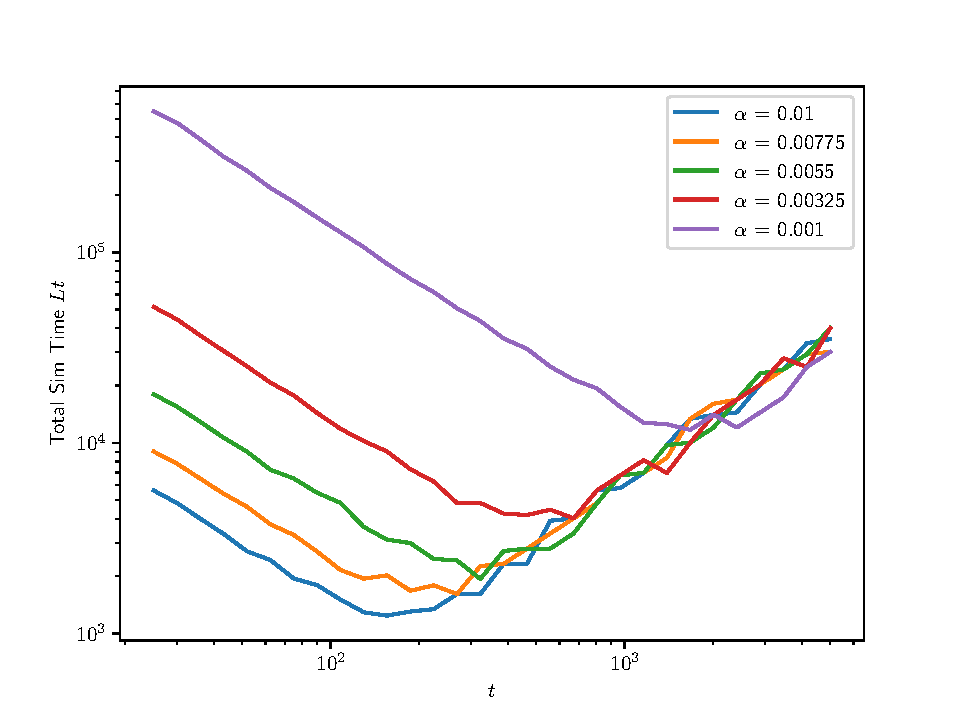
\includegraphics[width=0.75\linewidth]{numerics/data/single_qubit_tot_time_vs_t.pdf}
    \caption{Total simulation time for a single qubit system to reach within trace distance of $0.05$ of the thermal state for $\beta = 2$ as a function of per-interaction simulation time $t$. The slope of the large $t$ asymptote is $\approx$ 1.01.}\label{fig:tot_time_vs_single_time}
\end{figure}

The next task we have is to examine the $\beta$ dependence. For the harmonic oscillator Theorem \ref{thm:harmonic_oscillator} is helpful for giving an idea of the total simulation time for the ground state but we cannot extend it to finite $\beta$ due to the special structure of the transition matrix in the $\beta \to \infty$ limit. Perturbation theory could possibly be used to extend the computation of the spectral gap to the low temperature regime, but even then it would break down for large temperature (small $\beta$). For generic $\beta$ the structure of the harmonic oscillator transition matrix is tridiagonal but it is not quite Toeplitz, as the main diagonals deviate in the upper left and bottom right corners. We could try to pull these deviations into a separate matrix and treat them as perturbations to a fully Toeplitz matrix, which we can then compute the spectrum of. The issue with this approach is that these deviations are on the order of $\widetilde{\alpha}^2 q(0)$ and $\widetilde{\alpha}^2 q(1)$, which are comparable to the eigenvalues of the unperturbed matrix.

In Figure \ref{fig:sho_total_time_vs_beta} we are able to probe the total simulation time and spectral gap of the harmonic oscillator as a function of $\beta$. We reveal a rather surprising Mpemba-like phenomenon where it takes longer for an infinite temperature initial state (the maximally mixed state) to cool to intermediate temperatures than low temperature states. The Mpemba effect \cite{mpemba} is a classical phenomenon related to the time needed to freeze hot water compared to room temperature water with mentions going all the way back to Aristotle. This phenomenon has been extended to quantum thermodynamics and observed in both theory \cite{nickMpemba}, \cite{mpembaExplanation} and in recent experimental research \cite{zhang2025mpembaObservation}. Our observations are not only a further analytic observation, but we are able to provide a proposed mechanism that explains the behavior. It is clear that the distance of our initial state to the target thermal state $\norm{\rho_S(\beta) - \rho_S(\infty)}_1$ increases monotonically with $\beta$ but what is not obvious is that the spectral gap of the underlying Markov chain is \emph{also} increasing. As larger spectral gaps lead to quicker convergences this acts in an opposite way on the total simulation time. The end result is that for small $\beta$ the increase in initial distance is stronger than the increase in the spectral gap and $L \cdot t$ increases. After some amount of $\beta$ these forces flip and the spectral gap effects become stronger than the initial state distance increasing, leading to a reduction in $L \cdot t$. This phenomenon appears to become more pronounced as the dimension of the harmonic oscillator increases, as can be seem in the $\dim_S = 10$ data. Two things remain unclear: the first is what parameters affect the position and height of the peak in total simulation time and the second is if this behavior is present in Hamiltonians with more complicated eigenvalue difference structure than the harmonic oscillator.

\begin{figure}[t]
    \centering
    \begin{subfigure}{0.45\textwidth}
    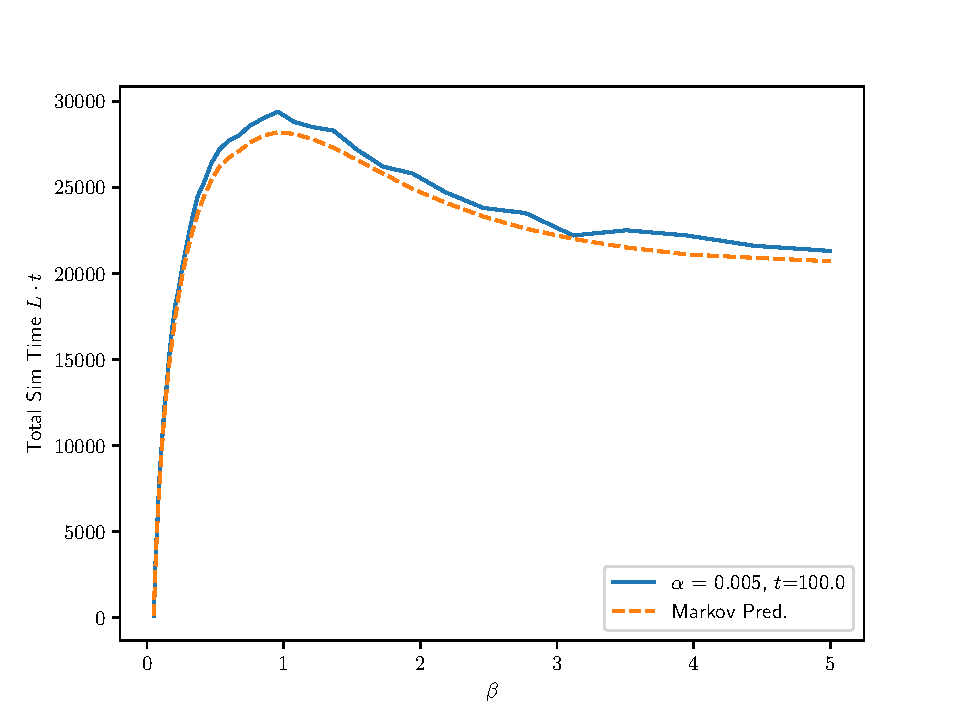
\includegraphics[width=\textwidth]{numerics/data/sho_total_time_vs_beta_dim_4.pdf}
    \caption{Minimum Interactions vs. $\beta$, $\dim = 4$}
    \label{fig:sho_l_vs_beta_dim_4}
    \end{subfigure}
    \begin{subfigure}{0.45\textwidth}
    \vspace{0.7cm}
    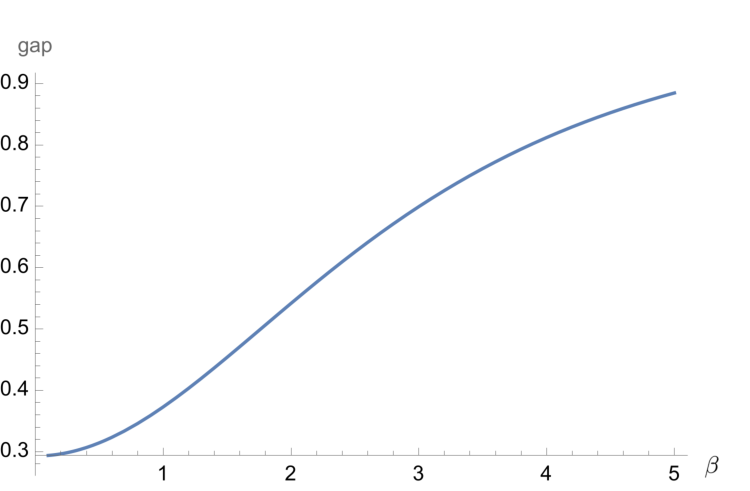
\includegraphics[width=\textwidth]{numerics/data/spec_gap_dim_4.pdf}
    \caption{Spectral Gap $\widetilde{\lambda}_\star(\beta)$ vs. $\beta$, $\dim = 4$}
    \label{fig:sho_spectral_gap_vs_beta}
    \end{subfigure}
    \hfill
    \begin{subfigure}{0.5\textwidth}
    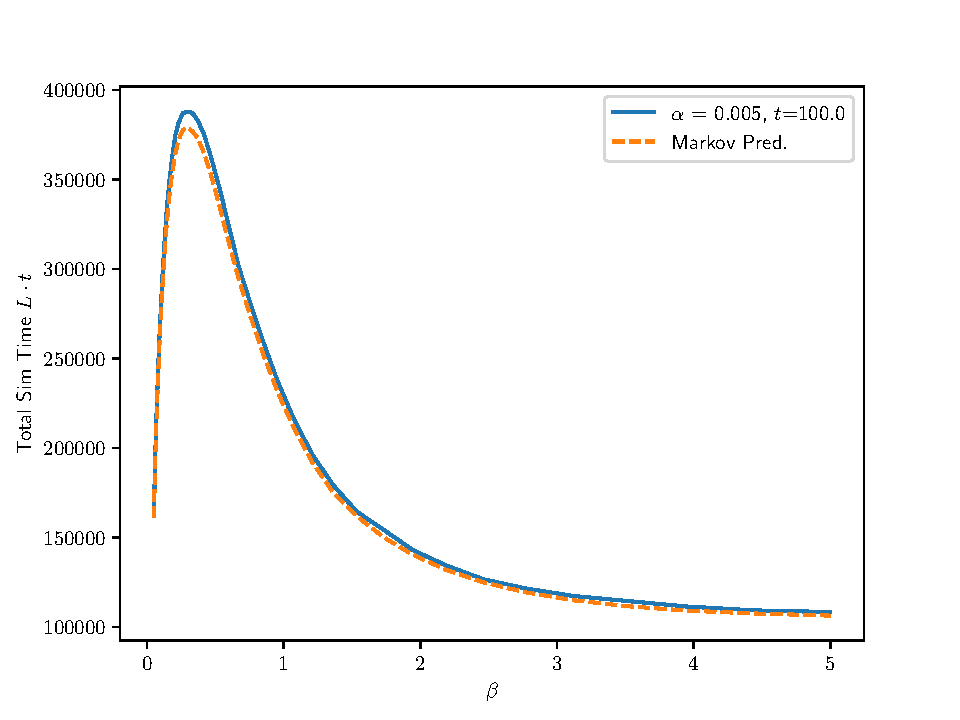
\includegraphics[width=\textwidth]{numerics/data/sho_total_time_vs_beta_dim_10.pdf}
    \caption{Total simulation time vs. $\beta$, $\dim = 10$}
    \label{fig:sho_l_vs_beta_dim_10}
    \end{subfigure}
    \caption{Demonstration of $\beta$ dependence of the thermalizing channel $\Phi$ for the truncated harmonic oscillator. The environment gap $\gamma$ was tuned to match the system gap $\Delta$ exactly. The minimal number of interactions was found by binary search over values of $L$ that have an average error of less than $\epsilon = 0.05$ with 100 samples.}
    \label{fig:sho_total_time_vs_beta}
\end{figure}

The analytic proofs given in Theorems \ref{thm:single_qubit} and \ref{thm:harmonic_oscillator} are entirely based on our weak-coupling expansion derived in Section \ref{sec:weak_coupling}. The high level picture of this expansion is that we have a remainder error that scales like $\bigo{(\alpha t)^3}$ and an off-resonance error that scales as $\bigo{\alpha^2}$. To balance these two terms we then set $\alpha = \bigo{1/t^3}$. However, as seen in Figure \ref{fig:tot_time_vs_single_time} our thermalization routine appears to be quite robust beyond this weak-coupling expansion, which could lead to significant improvements in runtime. In our derivation for the $\bigo{\alpha}$ and $\bigo{\alpha^2}$ terms we relied on our eigenvalues being I.I.D Gaussian variables, with the first and second order expressions containing factors with the first and second moments respectively of the Gaussian distribution. This would suggest that the third order term in a weak coupling expansion might also be 0, similarly to the first order term. This would lead to a supposed remainder error of $\bigo{\alpha^4 t^4}$, which after balancing with the off-resonance error would give $\alpha = \bigo{1/t^2}$. If the number of interactions then scales like $\bigo{1/\alpha^2 t^2}$, which is consistent with the spectral gap of $\TT_{\on}$ scaling as $\bigo{\alpha^2 t^2}$, then to make the total error of order $\bigo{\epsilon}$ we would require $t \in \bigotilde{1/\epsilon^{0.5}}$ as in Theorems \ref{thm:single_qubit} and \ref{thm:harmonic_oscillator}. This conjecture then leads to a total simulation time of order $\bigo{1/\epsilon^{1.5}}$. 

An even further conjecture would be to keep $\alpha \cdot t$ as a small constant, in this case we are essentially saying that the randomized dynamics $e^{i \alpha t G}$ are beneficial and should not be thought of as some remainder error to be minimized. If the $\alpha t$ constant is small enough then the dynamics will still be approximated by the Markov chain $\TT_{on}$. Our spectral gap will still scale as $\bigo{(\alpha t)^2}$ and $t$ as $\bigo{1/\epsilon^{0.5}}$. This would lead to our total simulation time scaling as $\bigo{1/\epsilon^{0.5}}$. In Figure \ref{fig:epsilon_scaling} we numerically explore these various scalings of $\alpha$ for the harmonic oscillator with $\beta = \dim_S = 4$. Our first remark is that the $\alpha = \bigo{1/t^3}$ scaling as dictated by Theorem \ref{thm:harmonic_oscillator} is numerically supported. 
 Specifically, the theorem suggests that we should observe $O(1/\epsilon^{2.5})$ scaling for $L\cdot t$. 
 Our experiment suggesting $L \cdot t \in \bigo{1/\epsilon^{2.764}}$ which is approximately consistent and deviations from this scaling may arise from the inclusion of data in the fit from outside of the weak coupling limit which is the only regime where we anticipate this scaling. 
 
 We obtained these exponents via least squares fitting of a power-law fit to $L\cdot t$ and $1/\epsilon$. 


\begin{figure}
    \centering
    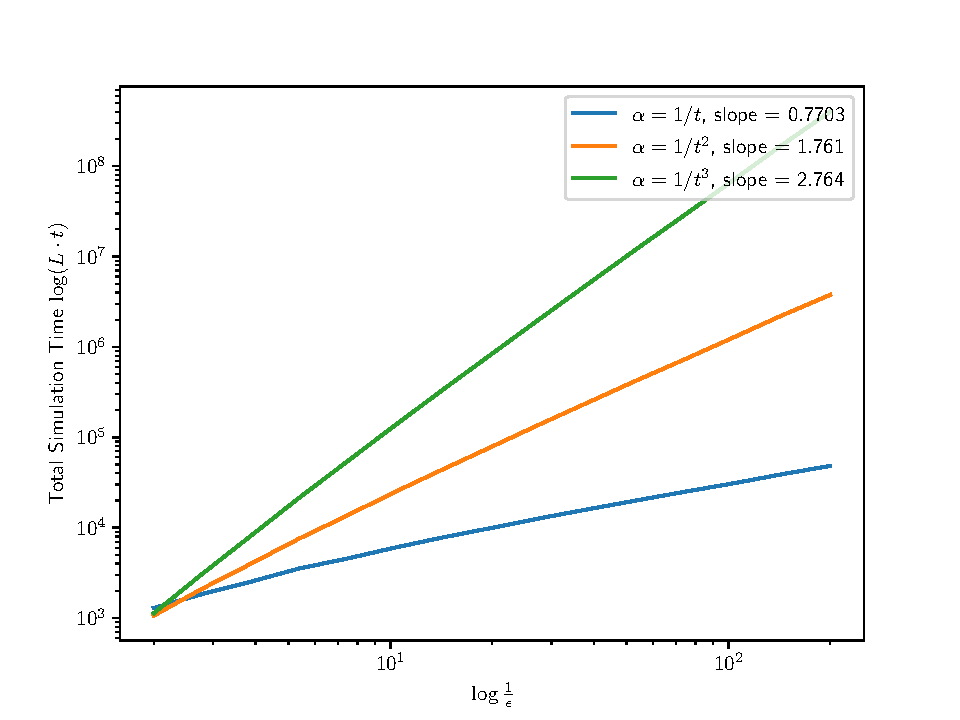
\includegraphics[width=0.66\linewidth]{numerics/data/epsilon_fitting_4.pdf}
    \caption{Scaling of $L \cdot t$ to prepare a harmonic oscillator thermal state with $\beta = \dim_S = 4$ with respect to $1/\epsilon$ in a log-log plot. For each line in the plot we scaled $\alpha$ by a constant value to make $\widetilde{\alpha}^2 \approx 0.05$ for the largest value of $\epsilon$. Each of these slopes is consistently larger by 0.25-0.27 compared to stated predictions.}
    \label{fig:epsilon_scaling}
\end{figure}


\section{General Systems} \label{sec:general_systems}

We now extend our thermalization techniques to arbitrary Hamiltonians with no degenerate eigenvalues. The first major difficulty that we run into is how to choose our environment gap $\gamma$. If one does not have any knowledge whatsoever about where the eigenvalues of $H_S$ may lie then we are reduced to uniform guessing. In Section \ref{sec:zero_knowledge} we show that even in this scenario the thermal state is an approximate fixed point for finite $\beta$ and the exact fixed point for ground states and we provide a bound on the total simulation time required. However, we show that this generality does come at a cost. If one has complete knowledge of the eigenvalue differences we show in Section \ref{sec:perfect_knowledge} that the total simulation time markedly decreases. Further, with complete knowledge the thermal state is an exact fixed point for all $\beta$. Finally, in Section \ref{sec:general_numerics} we study these impacts on small Hydrogen chain systems and observe the quantitative effects of noise added to $\gamma$. 

The assumption on non-degenerate eigenvalues is required for fairly technical conditions. In the $\beta \to \infty$ limit for our proof of the spectral gap we use the fact that the transition matrix $T$ is upper triangular in Lemma \ref{lem:fixed_point}. This is where the non-degeneracy is required because degenerate eigenvalues always have a non-zero transition amplitude that scales as $\bigo{\widetilde{\alpha}^2}$ without a factor of sinc. This means within the degenerate subspace in the transition matrix there is a uniform block. This makes computing the transition matrix spectrum a little more complicated than necessary, so we avoid this issue by requiring no degeneracies. This restriction could likely be lifted through an intelligent choice of eigenbasis for the degenerate subspace, or through better spectrum calculations of the resulting transition matrix, but we leave such explorations for future work. 



\subsection{Zero Knowledge} \label{sec:zero_knowledge}
We now move on to show how our channel performs if one has no knowledge about the eigenvalue differences $\Delta_S(i,j)$ apart from a bound on the maximum value of these differences. This is represented by choosing $\gamma$ uniformly from the interval $[0, 4 \norm{H_S}]$, which technically constitutes an upper bound on the largest $\Delta_S(i,j)$, but estimates of $\norm{H_S}$ are often readily attainable from the specification of the Hamiltonian using the triangle inequality.  We also assume that an input state that commutes with the Hamiltonian can be provided, the maximally mixed state is sufficient as would a random eigenstate yielded by the quantum phase estimation algorithm.

\begin{theorem}[Zero Knowledge Thermal State Prep] \label{thm:zero_knowledge}
    Let $H_S$ be a Hermitian matrix of dimension ${\rm dim}_S$ with no degenerate eigenvalues, $\rho$ any input state that commutes with $H_S$, and $\gamma$ a random variable distributed uniformly in the interval $[0, 4 \norm{H_S}]$ and
    let $\rho_{\rm fix}$ denote the unique fixed point of the transition dynamics $\identity + \EE_\gamma \TT_{\on}^{(\gamma)}$ where $\TT_{\on}^{(\gamma)}$ is the on-resonance transition matrix used above with the dependence on $\gamma$ made explicit. The following statements then hold.
    \begin{enumerate}
\item For finite $\beta$ the thermal state is an approximate fixed point of the thermalizing channel $\EE_\gamma \Phi_\gamma$ with a deviation of
    \begin{equation}
        \norm{\rho_S(\beta) - \EE_\gamma \Phi_\gamma(\rho_S(\beta))}_1 \le \alpha^2 t e^{\beta \delta_{\min}} \norm{H_S}^{-1} \pi + 8 \frac{\alpha^2}{\delta_{\min}} + 16 \sqrt{\frac{\pi}{2}} \dim_S (\alpha t)^3.
    \end{equation}
    \item   The parameter settings for any $\beta\in [0,\infty]$ and error tolerance $\epsilon \in (0,2]$
    \begin{align}
        \alpha = \frac{\delta_{\min}^4 \epsilon^{3} \widetilde{\lambda}_\star(\beta)^{3}}{\dim_S^7 \norm{H_S}^3}, ~t = \frac{\dim_S^2 \norm{H_S}}{\epsilon \widetilde{\lambda}_\star(\beta) \delta_{\min}^2}, \text{ and } L \in \bigotilde{\frac{\dim_S^{14} \norm{H_S}^6}{\epsilon^5 \delta_{\min}^6 \widetilde{\lambda}_\star(\beta)^{6} }}
    \end{align}
    are sufficient to guarantee $\norm{\rho_{\rm fix} - \left(\EE_\gamma \Phi_\gamma \right)^{\circ L}(\rho)}_1 \in \bigotilde{\epsilon}$.
    The total simulation time needed is therefore
    \begin{equation}
        L \cdot t \in \bigotilde{\frac{\dim_S^{16} \norm{H_S}^7}{\delta_{\min}^8 \epsilon^6 \widetilde{\lambda}_\star(\beta)^7}}.
    \end{equation}
   \item    The fixed point is the ground state In the $\beta \to \infty$ limit and the spectral gap, $\widetilde{\lambda}_\star(\beta)$, of the rescaled transition matrix $\EE_\gamma T_\gamma \cdot \left(\frac{2 \norm{H_S} (\dim + 1)}{\alpha^2 t}\right)$ is lower bounded by a constant, giving the two limits
    \begin{equation}
        \lim_{\beta \to \infty} \rho_{\rm fix} = \ketbra{1}{1} \text{ and } \lim_{\beta \to \infty} \widetilde{\lambda}_\star(\beta) = 2 \int_{0}^{-\delta_{\min}t/2} \sinc^2(u) du \ge 2.43.
        \end{equation}

    \end{enumerate}
\end{theorem}
\begin{proof}
    %This proof structure will be structurally similar to the proof of Theorem \ref{thm:perfect_knowledge}. 
    We start by understanding the fixed points of $\identity + \EE_\gamma \TT_{\on}^{(\gamma)}$, conditions for the thermal state being fixed are given in Lemma \ref{lem:fixed_point}. As the condition boils down to a detailed balance like condition, we need to compute the off-diagonal transition elements first. Starting with $i > j$ we have from Definition~\ref{def:transition} that
    \begin{align}
        &\EE_\gamma \bra{j} \TT_{\on}^{(\gamma)}(\ketbra{i}{i})\ket{j} \nonumber \\
        &=  \widetilde{\alpha}^2 \EE_{\gamma} \frac{1}{1 + e^{-\beta \gamma}} \mathbf{I}[|\Delta_S(i,j) - \gamma| \le \delta_{\min}]  \sinc^2\left(\frac{(\Delta_S(i,j) - \gamma)t}{2}\right) \\ \nonumber \\
        &~+ \widetilde{\alpha}^2 \EE_{\gamma} \frac{e^{-\beta \gamma}}{1 + e^{-\beta \gamma}} \mathbf{I}[|\Delta_S(i,j) + \gamma| \le \delta_{\min}]  \sinc^2\left(\frac{(\Delta_S(i,j) + \gamma)t}{2}\right) \\
        &= \widetilde{\alpha}^2 \EE_{\gamma} \frac{1}{1 + e^{-\beta \gamma}} \mathbf{I}[|\Delta_S(i,j) - \gamma| \le \delta_{\min}]  \sinc^2\left(\frac{(\Delta_S(i,j) - \gamma)t}{2}\right) \\
        &= \widetilde{\alpha}^2 \frac{1}{4 \norm{H_S}} \int_{0}^{4 \norm{H_S}} \frac{1}{1 + e^{-\beta \gamma}} \mathbf{I}[|\Delta_S(i,j) - \gamma| \le \delta_{\min}]  \sinc^2\left(\frac{(\Delta_S(i,j) - \gamma)t}{2}\right) d\gamma \\
        &=  \frac{\widetilde{\alpha}^2}{4 \norm{H_S}} \int_{\Delta_S(i,j) - \delta_{\min}}^{\Delta_S(i,j) + \delta_{\min}} \frac{1}{1 + e^{-\beta \gamma}}  \sinc^2\left(\frac{(\Delta_S(i,j) - \gamma)t}{2}\right) d\gamma \\
        &= \frac{\widetilde{\alpha}^2}{2 t \norm{H_S}} \int_{-\delta_{\min} t /2}^{\delta_{\min} t / 2} \frac{1}{1 + e^{-\beta (\Delta_S(i, j) - 2 u /t)}} \sinc^2(u) du. \label{eq:zero_knowledge_transition_1}
    \end{align}
    The exact same calculation holds for $i < j$, which after repeating the steps that led to~\eqref{eq:zero_knowledge_transition_1} we arrive at a similar result  with a slightly different integrand
    \begin{align}
        \EE_\gamma \bra{j} \TT_{\on}^{(\gamma)}(\ketbra{i}{i})\ket{j} &= \frac{\widetilde{\alpha}^2}{2 t \norm{H_S}} \int_{-\delta_{\min} t /2}^{\delta_{\min} t / 2} \frac{e^{-\beta (\Delta_S(j,i) - 2 u /t)}}{1 + e^{-\beta (\Delta_S(j,i) - 2 u /t)}} \sinc^2(u) du,\label{eq:zero_knowledge_transition_2}
    \end{align}
    as we pick up a factor of $q(1)$ as opposed to $q(0)$. Note that we have also shown that $\EE_\gamma T_\gamma$ is ergodic, as there is a nonzero probability for any state $\ketbra{i}{i}$ to transition to any other state $\ketbra{j}{j}$ in one iteration on average over $\gamma$.

    For finite $\beta$ the condition for $\rho_S(\beta)$ being a fixed point is given in Eq. \eqref{eq:detailed_balance}, repeated here as
    \begin{equation}
        \sum_{i \neq j} \frac{e^{-\beta \lambda_S(i)}}{\partfun_S(\beta)} e_j^T \EE_\gamma T_\gamma e_i - \frac{e^{-\beta \lambda_S(j)}}{\partfun_S(\beta)}  e_i^T \EE_\gamma T_\gamma e_j = 0,
    \end{equation}
    for all $j$. We can plug in our calculation for the transition coefficients for summands with $i > j$ first
    \begin{align}
        &\frac{e^{-\beta \lambda_S(i)}}{\partfun_S(\beta)} e_j^T \EE_\gamma T_\gamma e_i - \frac{e^{-\beta \lambda_S(j)}}{\partfun_S(\beta)}  e_i^T \EE_\gamma T_\gamma e_j \nonumber \\ 
        &= \frac{e^{-\beta \lambda_S(j)}}{\partfun_S(\beta)} \left( e^{-\beta \Delta_S(i,j)} \EE_\gamma \bra{j} \TT_{\on}^{(\gamma)}(\ketbra{i}{i})\ket{j} - \bra{i} \TT_{\on}^{(\gamma)}(\ketbra{j}{j})\ket{i} \right) \\
        &= \frac{e^{-\beta \lambda_S(j)}}{\partfun_S(\beta)} \frac{\widetilde{\alpha}^2}{2 t \norm{H_S}} e^{-\beta \Delta_S(i,j)} \int_{-\delta_{\min} t /2 }^{\delta_{\min} t/ 2} \frac{1 - e^{\beta 2 u / t}}{1 + e^{-\beta(\Delta_S(i,j) - 2u/t)}} \sinc^2(u) du \\
        &= \frac{e^{-\beta \lambda_S(i)}}{\partfun_S(\beta)} \frac{\widetilde{\alpha}^2}{2 t \norm{H_S}} \int_{-\delta_{\min} t /2 }^{\delta_{\min} t/ 2} \frac{1 - e^{\beta 2 u / t}}{1 + e^{-\beta(\Delta_S(i,j) - 2u/t)}} \sinc^2(u) du. \label{eq:zero_knowledge_tmp_1}
    \end{align}
    For $i < j$ we have the very similar
    \begin{align}
        &\frac{e^{-\beta \lambda_S(i)}}{\partfun_S(\beta)} e_j^T \EE_\gamma T_\gamma e_i - \frac{e^{-\beta \lambda_S(j)}}{\partfun_S(\beta)}  e_i^T \EE_\gamma T_\gamma e_j \nonumber \\ 
        &= \frac{e^{-\beta \lambda_S(j)}}{\partfun_S(\beta)} \frac{\widetilde{\alpha}^2}{2 t \norm{H_S}} \int_{-\delta_{\min} t /2 }^{\delta_{\min} t/ 2} \frac{ e^{\beta 2 u / t} - 1}{1 + e^{-\beta(\Delta_S(j, i) - 2u/t)}} \sinc^2(u) du. \label{eq:zero_knowledge_tmp_2}
    \end{align}
    Unfortunately these integrals are not 0, which can be verified numerically, and it is unclear how to make the summation over $i \neq j$ equal to 0. 
    
    Our work around this is that instead of showing that the thermal state is exactly the fixed point we can use these results to show that it is an approximate fixed point. There are a few ways we could proceed. The first way could be to compute a Taylor series for the integrand and isolate the limits in which the remainder goes to 0. Unfortunately due to the $\sinc^2(u) = \sin(u)^2 / u^2$ term this means that the overall scaling will go like $1/t$, making the total expression independent of $t$. Instead the route we will take will be to upper bound the norm $\norm{\vec{p}_{\beta} - \EE_\gamma (I + T_\gamma)\vec{p}_\beta}_1 = \norm{\EE_\gamma T_\gamma \vec{p}_\beta}_1$, as this norm is only 0 if $\vec{p}_\beta$ is a fixed point. We reduce this to computations we have already performed as
    \begin{align}
        \norm{\EE_\gamma T_\gamma \vec{p}_\beta}_1 &= \sum_j \abs{e_j^T \EE_\gamma T_\gamma \vec{p}_\beta } \\
        &= \sum_j \abs{\sum_{i} \frac{e^{-\beta \lambda_S(i)}}{\partfun_S(\beta)} e_j^T \EE_\gamma T_\gamma e_i } \\
        &= \sum_j \abs{\sum_{i \neq j} \frac{e^{-\beta \lambda_S(i)}}{\partfun_S(\beta)} e_j^T \EE_\gamma T_\gamma e_i - \frac{e^{-\beta \lambda_S(j)}}{\partfun_S(\beta)} e_i^T \EE_\gamma T_\gamma e_j}.
    \end{align}
    This is essentially the derivation for the fixed point conditions described in Lemma \ref{lem:fixed_point}. We now plug in Eqs. \eqref{eq:zero_knowledge_tmp_1} and \eqref{eq:zero_knowledge_tmp_2} into the above and upper bound the integral as
    \begin{align}
        &\sum_j \abs{\sum_{i \neq j} \frac{e^{-\beta \lambda_S(i)}}{\partfun_S(\beta)} e_j^T \EE_\gamma T_\gamma e_i - \frac{e^{-\beta \lambda_S(j)}}{\partfun_S(\beta)} e_i^T \EE_\gamma T_\gamma e_j} \nonumber \\
        &\le \sum_j \abs{\sum_{i < j} \frac{e^{-\beta \lambda_S(i)}}{\partfun_S(\beta)} e_j^T \EE_\gamma T_\gamma e_i - \frac{e^{-\beta \lambda_S(j)}}{\partfun_S(\beta)} e_i^T \EE_\gamma T_\gamma e_j} + \sum_j  \abs{\sum_{i > j} \frac{e^{-\beta \lambda_S(i)}}{\partfun_S(\beta)} e_j^T \EE_\gamma T_\gamma e_i - \frac{e^{-\beta \lambda_S(j)}}{\partfun_S(\beta)} e_i^T \EE_\gamma T_\gamma e_j} \\
        &= \frac{\widetilde{\alpha}^2}{2 t \norm{H_S}} \sum_j \abs{\sum_{i < j} \frac{e^{-\beta \lambda_S(j)}}{\partfun_S(\beta)} \int_{-\delta_{\min} t /2 }^{\delta_{\min} t/ 2} \frac{ e^{\beta 2 u / t} - 1}{1 + e^{-\beta(\Delta_S(j, i) - 2u/t)}} \sinc^2(u) du} \nonumber \\
        &+ \frac{\widetilde{\alpha}^2}{2 t \norm{H_S}} \sum_j  \abs{\sum_{i > j} \frac{e^{-\beta \lambda_S(i)}}{\partfun_S(\beta)} \int_{-\delta_{\min} t /2 }^{\delta_{\min} t/ 2} \frac{1 - e^{\beta 2 u / t}}{1 + e^{-\beta(\Delta_S(i,j) - 2u/t)}} \sinc^2(u) du} \\
        &\le \frac{\widetilde{\alpha}^2}{2 t \norm{H_S}} \sum_j \sum_{i < j} \frac{e^{-\beta \lambda_S(j)}}{\partfun_S(\beta)} \int_{-\delta_{\min} t /2 }^{\delta_{\min} t/ 2}\abs{ \frac{ e^{\beta 2 u / t} - 1}{1 + e^{-\beta(\Delta_S(j, i) - 2u/t)}}} \sinc^2(u) du \nonumber \\
        &+ \frac{\widetilde{\alpha}^2}{2 t \norm{H_S}} \sum_j  \sum_{i > j} \frac{e^{-\beta \lambda_S(i)}}{\partfun_S(\beta)} \int_{-\delta_{\min} t /2 }^{\delta_{\min} t/ 2} \abs{ \frac{1 - e^{\beta 2 u / t}}{1 + e^{-\beta(\Delta_S(i,j) - 2u/t)}} } \sinc^2(u) du \\
        &\le \frac{\widetilde{\alpha}^2}{2 t \norm{H_S}} e^{\beta \delta_{\min}} \int_{-\delta_{\min}t/2}^{\delta_{\min}t /2} \sinc^2(u) du \left(\sum_j \frac{e^{-\beta \lambda_S(j)}}{\partfun_S(\beta)} \sum_{i < j} 1 + \sum_j \sum_{i > j} \frac{e^{-\beta \lambda_S(i)}}{\partfun_S(\beta)}  \right) \\
        &\le \frac{\widetilde{\alpha}^2 \dim_S}{t \norm{H_S}} e^{\beta \delta_{\min}} \pi \\
        &\le \alpha^2 t e^{\beta \delta_{\min}} \norm{H_S}^{-1} \pi.
    \end{align}
    For this we can have $\alpha t$, which represents the total simulation time multiplied by the strength of the random interaction $G$, be constant and still take $\alpha \to 0$ to achieve arbitrarily small error.

    Now we turn to bounding the total simulation time. We will let $\rho_{\rm fix}$ denote the fixed point of the dynamics. As before, we break the error into two pieces
    \begin{equation}
        \norm{\rho_{\rm fix} - \left(\EE_\gamma \Phi_\gamma \right)^{\circ L}}_1 \le \norm{\rho_{\rm fix} - \left(\EE_\gamma \identity + \TT_{\on}^{(\gamma)}\right)^{\circ L} (\rho)}_1 + L(\norm{\TT_{\off}}_1 + \norm{R_{\Phi}}_1).
    \end{equation}
    Let $\widetilde{\lambda}_\star(\beta)$ denote the spectral gap for the rescaled transition matrix $\EE_\gamma T_\gamma \cdot \left(\frac{2 \norm{H_S} (\dim + 1)}{\alpha^2 t}\right)$, as this is the dimensionful prefactor in front of the transitions derived in Eqs. \eqref{eq:zero_knowledge_transition_1} and \eqref{eq:zero_knowledge_transition_2}. Jerison's Markov Relaxation Theorem \ref{thm:markov_chain_bound} tells us that taking $L$ to satisfy
    \begin{equation}
        L \ge \frac{\dim_S}{\lambda_\star} J \in \bigotilde{\frac{\dim_S^2 \norm{H_S}}{\alpha^2 t \widetilde{\lambda}_\star(\beta)}}\label{eq:Lbd}
    \end{equation}
    is sufficient to guarantee $\norm{\rho_{\rm fix} - \left(\EE_\gamma \identity + \TT_{\on}^{(\gamma)}\right)^{\circ L} (\rho)}_1 \in \bigotilde{\epsilon}$. Now we balance the off-resonance and remainder errors
    \begin{equation}
        \norm{\TT_{\off}}_1 + \norm{R_{\Phi}}_1 \le \frac{8 \alpha^2}{\delta_{\min}^2} + 16 \sqrt{\frac{\pi}{2}} \dim_S (\alpha t)^3 = \frac{\alpha^2}{\delta_{\min}^2} \left( 8 + 16 \sqrt{\frac{\pi}{2}} \dim_S \alpha \delta_{\min}^2 t^3 \right),
    \end{equation}
    and we see setting $\alpha = \frac{1}{\dim_S \delta_{\min}^2 t^3}$ makes the parenthesis a constant.
    To bound the total off-resonance and remainder error we take the product
    \begin{equation}
        L(\norm{\TT_{\off}}_1 + \norm{R_{\Phi}}_1) \in \bigotilde{\frac{\dim_S^2 \norm{H_S}}{\alpha^2 t \widetilde{\lambda}_\star(\beta)} \frac{\alpha^2}{\delta_{\min}^2}} = \bigotilde{\frac{\dim_S^2 \norm{H_S}}{ t \delta_{\min}^2 \widetilde{\lambda}_\star(\beta)} }.
    \end{equation}
    Observe that setting 
    \begin{equation}
        t = \frac{\dim_S^2 \norm{H_S}}{\epsilon \delta_{\min}^2 \widetilde{\lambda}_\star(\beta)}
    \end{equation} 
    is sufficient to make the above product $L(\norm{\TT_{\off}}_1 + \norm{R_{\Phi}}_1) \in\bigotilde{\epsilon}$. 

    We now turn to the $\beta \to \infty$ limit. For this we note that Lemma \ref{lem:fixed_point} guarantees that the ground state is a fixed point and that $\EE_\gamma T_\gamma$ is upper triangular. We will show the ground state is unique by computing the spectrum of $\EE_\gamma T_\gamma$. For this we take the $\beta \to \infty$ limit of the transitions in Eqs. \eqref{eq:zero_knowledge_transition_1} and \eqref{eq:zero_knowledge_transition_2}, which will give us the diagonal elements and then the spectrum. Starting with $i > j$ given in Eq. \eqref{eq:zero_knowledge_transition_1} we get
    \begin{align}
        \lim_{\beta \to \infty} \EE_\gamma \bra{j} \TT_{\on}^{(\gamma)}(\ketbra{i}{i})\ket{j} &= \frac{\widetilde{\alpha}^2}{2 t \norm{H_S}} \int_{-\delta_{\min}t/2}^{\delta_{\min}t/2} \sinc^2(u) du
    \end{align}
    and for $i < j$ from Eq. \eqref{eq:zero_knowledge_transition_2} we have
    \begin{equation}
        \lim_{\beta \to \infty} \EE_\gamma \bra{j} \TT_{\on}^{(\gamma)}(\ketbra{i}{i})\ket{j} = 0.
    \end{equation}
    We denote the $\sinc$ integration above as
    \begin{equation}
        I_{\sinc}(t) \coloneqq \int_{-\delta_{\min}t/2}^{\delta_{\min} t/2} \sinc^2(u) du,
    \end{equation}
    and we will show later that this is constant for $\dim_S \ge 3$. Now these transitions allow us to compute the diagonal elements
    \begin{align}
        \lim_{\beta \to \infty} \EE_\gamma \bra{i} \TT_{\on}^{(\gamma)}(\ketbra{i}{i}) \ket{i} &= - \sum_{j \neq i} \lim_{\beta \to \infty} \EE_\gamma \bra{j} \TT_{\on}^{(\gamma)}(\ketbra{i}{i}) \ket{j} \\
        &= - \sum_{j < i} \lim_{\beta \to \infty} \EE_\gamma \bra{j} \TT_{\on}^{(\gamma)}(\ketbra{i}{i}) \ket{j} \\
        &= - \frac{\widetilde{\alpha}^2}{2 t \norm{H_S}} (i - 1) I_{\sinc}(t).
    \end{align}
    This gives a spectrum for $\EE_\gamma T_\gamma$ as 0 and $- \frac{\widetilde{\alpha}^2}{2 t \norm{H_S}} (i - 1) I_{\sinc}(t)$ for $i > 1$. This shows the ground state is the unique fixed point as 0 has multiplicity 1 in the spectrum. Further the spectral gap of the rescaled transition matrix $\widetilde{\lambda}_\star(\beta)$ is then given by
    \begin{equation}
        \lim_{\beta \to \infty} \widetilde{\lambda}_\star(\beta) = I_{\sinc}(t).
    \end{equation}
    We can repeat the analysis for finding suitable values for $\alpha, t, $ and $L$ to guarantee thermalization and we find that 
    \begin{equation}
        \alpha = \frac{1}{\dim_S \delta_{\min}^2 t^3}, ~ t = \frac{4 \dim_S^2 \norm{H_S}}{\epsilon \delta_{\min}^2}, \text{ and } L \in \bigotilde{\frac{\dim_S^2 \norm{H_S}}{\alpha^2 t}}
    \end{equation}
    are sufficient to guarantee $\norm{\ketbra{1}{1} - \left( \EE_\gamma \Phi_\gamma\right)^{\circ L} (\rho)}_1 \in \bigotilde{\epsilon}$.  Substituting this into~\eqref{eq:Lbd} yields
    \begin{equation}
        L\cdot t \in \bigotilde{\frac{\dim_S^{16} \norm{H_S}^7}{\delta_{\min}^8 \epsilon^6 \widetilde{\lambda}_\star(\beta)^7}}
    \end{equation}
    as stated in the second claim in the theorem.

    Our final task is to justify the third claim of the theorem, which involves showing that $I_{\sinc}(t)$ as constant is valid. Using the choice of $t$ directly above
    \begin{align}
        I_{\sinc}(t) = \int_{-\delta_{\min} t /2}^{\delta_{\min} t /2}  \sinc^2(u) du = 2 \int_{0}^{ \frac{\dim_S^2 4 \norm{H_S}} {\epsilon \delta_{\min}}} \sinc^2(u) du. \label{eq:zero_knowledge_sinc_integral}
    \end{align}
    Now we note that this integral is monotonic with respect to the upper limit of integration with a final value of $\lim_{t \to \infty} I_{\sinc}(t) = \pi$. We note that we can capture a significant amount of this integral by just requiring the upper limit to be greater than the first zero of sinc located at $\frac{\pi}{2}$, which is true if $\epsilon \le \frac{4 \dim_S^2 \norm{H_S}}{\pi \delta_{\min}}$. This value can be computed as $2 \int_0^{\pi / 2} \sinc^2(u) du \ge 2.43$. This can be guaranteed by noting that $\epsilon$ can be at most 2, so the upper limit in Eq. \eqref{eq:zero_knowledge_sinc_integral} is satisfied if
    \begin{align}
    \epsilon \le 2 \le \frac{3^2}{\pi} \le \frac{\dim_S^2}{\pi} \le \frac{\dim_S^2 4 \norm{H_S}}{\pi \delta_{\min}},
\end{align}
as $\delta_{\min} \le 4 \norm{H_S}$. This shows that for our choice of $t$ then $|I_{\sinc}(t) - \pi| \le 0.71$, rendering it asymptotically constant as claimed.
\end{proof}

There are a few points that need to be addressed with the above theorem. The first is that our proof of the approximate fixed point utilizes rather poor bounds, resulting in diverging behavior as $\beta \to \infty$. For finite $\beta$ our bounds on the change in the thermal state scales as $e^{\beta \delta_{\min}}$, which diverges as $\beta$ goes to $\infty$, but in this exact same limit we are able to show that the ground state is the \emph{exact} fixed point of the Markov chain. This clear divergence in approximation error is a result of loose bounds and could be a potential avenue for improvement. The second point we would like to address is the rather high asymptotic scaling. This is the byproduct of a few things, the most important of which is the introduction of a $1/t$ in the reduction of the $\sinc$ integral. This causes a downstream effect of increasing the degree of each asymptotic parameter. To improve this one would need some kind of knowledge of the eigenvalues to prevent a uniform integration of each $\sinc$ term. We study the limiting case of this by assuming sample access to the exact eigenvalue differences $\Delta_S(i,j)$ in Section \ref{sec:perfect_knowledge} and obtain much improved scaling. The second source of inflation in our asymptotic scaling could be our weak-coupling approach to studying the channel. As explored numerically in Section \ref{sec:specific_numerics} we find that using different $\alpha$ scalings with respect to $t$ can greatly effect the $\epsilon$ scaling of the total simulation time $L \cdot t$. A higher order analysis of this channel could lead to anytically better guarantees on the thermalization time required, even in this zero knowledge scenario.

\subsection{Perfect Knowledge} \label{sec:perfect_knowledge}

Oftentimes when studying a system some knowledge of the eigenvalue gaps may be present. Our goal in this section is to study the extreme case of this scenario where one has knowledge of the exact eigenvalue differences. This is unlikely to happen with realistic quantum materials but instead serves as an ideal scenario for our channel to benchmark the effects of eigenvalue knowledge. Further, we note for some computational tasks, such as amplitude amplification, the eigenvalues may be explicitly computable and the real task is to find the dominant eigenvectors. A more realistic model for studying the impacts of eigenvalue knowledge on the total simulation time might be to place Gaussians at each of the $\Delta_S(i,j)$ values with some width $\sigma$. This is the model we use for numeric investigations in Section \ref{sec:general_numerics}, but we were unable to compute the total simulation time required analytically. We find that our model of perfect knowledge allows us to show a reduced total simulation time budget, with the ratio of zero knowledge to perfect knowledge scaling as $\bigotilde{\frac{\norm{H_S}^7}{\delta_{\min}^7 \epsilon^{3.5} \widetilde{\lambda}_\star(\beta)^{3.5}}}$, 
     which gives an explicit worst-case simulation time bound for ground state preparation.




\begin{theorem}[Perfect Knowledge Thermal State Prep] \label{thm:perfect_knowledge}
    Let $H_S$ be a Hermitian matrix of dimension ${\rm dim}_S$ with no degenerate eigenvalues, $\rho$ any input state that commutes with $H_S$ , and let $\gamma$ be a random variable with distribution $\prob{\gamma = \Delta(i,j)} = \frac{\eta_\Delta(i,j)}{\binom{\dim_S}{2}}$ where $\eta_{i,j}$ is the number of times a particular eigenvalue difference appears. For any $\beta\in [0,\infty]$ the thermal state can be prepared with controllable error
    \begin{equation}
        \norm{\rho_S(\beta) - \left(\EE_\gamma \Phi_\gamma \right)^{\circ L}(\rho)}_1 \in \bigotilde{\epsilon}
    \end{equation}
     with the following parameter settings
     \begin{align}
         \alpha &= \frac{\delta_{\min} \epsilon^{1.5} \widetilde{\lambda}_\star(\beta)^{1.5}}{\dim_S^7}, t = \frac{\dim_S^2}{\delta_{\min} \epsilon^{0.5} \widetilde{\lambda}_\star(\beta)^{0.5}},\text{ and } L \in \bigotilde{\frac{\dim_S^{14}}{\epsilon^2 \widetilde{\lambda}_\star(\beta)^3}},
     \end{align}
     where $\widetilde{\lambda}_\star(\beta)$ is the spectral gap of the rescaled transition matrix $\EE_\gamma T_\gamma  \cdot \frac{\binom{\dim_S}{2}}{\widetilde{\alpha}^2}$. 
     This gives the total simulation time required as
     \begin{equation}
         L \cdot t \in \bigotilde{\frac{\dim_S^{16}}{\delta_{\min} \epsilon^{2.5} \widetilde{\lambda}_\star(\beta)^{3.5}}}.
     \end{equation}
     All of the above conditions hold in the ground state limit as $\beta \to \infty$ and further we can compute a lower bound on the spectral gap of the rescaled transition matrix as
     \begin{equation}
         \lim_{\beta \to \infty} \widetilde{\lambda}_\star(\beta) = \min_{i > 1} \sum_{j < i} \eta_\Delta(i,j) \ge 1.
     \end{equation}
\end{theorem}
\begin{proof}
This proof structure is structurally similar to the proof of Theorem \ref{thm:zero_knowledge}.
To show that the thermal state is the fixed point we will need to compute transition factors of the form $\EE_\gamma \bra{j}\TT_{\on}^{(\gamma)}(\ketbra{i}{i})\ket{j}$ for use in Lemma \ref{lem:fixed_point}. Using the on-resonance definition in Eq. \eqref{eq:on_resonance} we have for $i > j$
\begin{align}
    &\EE_\gamma \bra{j} \TT_{\on}^{(\gamma)}(\ketbra{i}{i})\ket{j} \nonumber \\
    &=  \widetilde{\alpha}^2 \EE_{\gamma} \frac{1}{1 + e^{-\beta \gamma}} \mathbf{I}[|\Delta_S(i,j) - \gamma| \le \delta_{\min}]  \sinc^2\left(\frac{(\Delta_S(i,j) - \gamma)t}{2}\right) \nonumber \\
    &~+ \widetilde{\alpha}^2 \EE_{\gamma} \frac{e^{-\beta \gamma}}{1 + e^{-\beta \gamma}} \mathbf{I}[|\Delta_S(i,j) + \gamma| \le \delta_{\min}]  \sinc^2\left(\frac{(\Delta_S(i,j) + \gamma)t}{2}\right) \\
    &= \widetilde{\alpha}^2 \sum_{\Delta_S(k,l)} \prob{\gamma = \Delta_S(k,l)} \frac{\mathbf{I}[|\Delta_S(i,j) - \Delta_S(k,l)| \le \delta_{\min}]}{1 + e^{-\beta \Delta_S(k,l)}}   \sinc^2\left(\frac{(\Delta_S(i,j) - \Delta_S(k,l))t}{2}\right) \\
    &= \widetilde{\alpha}^2 \frac{\eta_\Delta(i,j)}{\binom{\dim_S}{2}} \frac{1}{1 + e^{-\beta \Delta_S(i,j)}}.
\end{align}
$i < j$ can be computed similarly as
\begin{equation}
    \EE_\gamma \bra{j} \TT_{\on}^{(\gamma)}(\ketbra{i}{i})\ket{j} = \widetilde{\alpha}^2 \frac{\eta_\Delta(i,j)}{\binom{\dim_S}{2}} \frac{e^{-\beta \Delta_S(k,l)}}{1 + e^{-\beta \Delta_S(k,l)}}.
\end{equation}
This allows us to compute the detailed-balance like condition in Eq. \eqref{eq:detailed_balance} for $i > j$
\begin{align}
    &\frac{e^{-\beta \lambda_S(i)}}{\partfun_S(\beta)} \EE_\gamma \bra{j} \TT_{\on}^{(\gamma)}(\ketbra{i}{i}) \ket{j} - \frac{e^{-\beta \lambda_S(j)}}{\partfun_S(\beta)} \bra{i} \TT_{\on}^{(\gamma)}(\ketbra{j}{j}) \ket{i} \nonumber \\
    &= \frac{e^{-\beta \lambda_S(i)}}{\partfun_S(\beta)} \widetilde{\alpha}^2 \frac{\eta_\Delta(i,j)}{\binom{dim_S}{2}} \frac{1}{1 + e^{-\beta \Delta_S(i,j)}} - \frac{e^{-\beta \lambda_S(j)}}{\partfun_S(\beta)} \widetilde{\alpha}^2 \frac{\eta_\Delta(i,j)}{\binom{dim_S}{2}} \frac{e^{-\beta \Delta_S(i,j)}}{1 + e^{-\beta \Delta_S(i,j)}} \\
    &= \frac{\widetilde{\alpha}^2}{\partfun_S(\beta)} \frac{\eta_\Delta(i,j)}{\binom{\dim_S}{2}} \left(\frac{e^{-\beta \lambda_S(i)}}{1 + e^{-\beta \Delta_S(i,j)}} - e^{-\beta \lambda_S(j)} \frac{e^{-\beta \Delta_S(i,j)}}{1 + e^{-\beta \Delta_S(i,j)} } \right) \\
    &= 0.
\end{align}
For $i < j$ we can repeat the same steps to argue that detailed balance also holds in this case.
\begin{align}
    &\frac{e^{-\beta \lambda_S(i)}}{\partfun_S(\beta)} \EE_\gamma \bra{j} \TT_{\on}^{(\gamma)}(\ketbra{i}{i}) \ket{j} - \frac{e^{-\beta \lambda_S(j)}}{\partfun_S(\beta)} \bra{i} \TT_{\on}^{(\gamma)}(\ketbra{j}{j}) \ket{i} \nonumber \\
    &= \frac{e^{-\beta \lambda_S(i)}}{\partfun_S(\beta)} \widetilde{\alpha}^2 \frac{\eta_\Delta(i,j)}{\binom{dim_S}{2}} \frac{e^{-\beta \Delta_S(j, i)}}{1 + e^{-\beta \Delta_S(j, i)}} - \frac{e^{-\beta \lambda_S(j)}}{\partfun_S(\beta)} \widetilde{\alpha}^2 \frac{\eta_\Delta(i,j)}{\binom{dim_S}{2}} \frac{1}{1 + e^{-\beta \Delta_S(j, i)}} \\
    &= \frac{\widetilde{\alpha}^2}{\partfun_S(\beta)} \frac{\eta_\Delta(i,j)}{\binom{\dim_S}{2}} \left(\frac{e^{-\beta \lambda_S(j)}}{1 + e^{-\beta \Delta_S(j, i)}} - \frac{e^{-\beta \lambda_S(j)}}{1 + e^{-\beta \Delta_S(j, i)} } \right) \\
    &= 0.
\end{align}
This is sufficient to show that the thermal state $\rho_S(\beta)$ is a fixed point via Lemma \ref{lem:fixed_point}. As we have also shown that the probability of transitioning from any state $\ketbra{i}{i}$ to any other state $\ketbra{j}{j}$ is nonzero this gives a nonzero expected hitting time for any pair of states. This implies the Markov chain is ergodic and that $\rho_S(\beta)$ is the \emph{unique} fixed point.

Next we bound the total simulation time required. For reasons similar to the harmonic oscillator in Section \ref{sec:harmonic_oscillator} we are unable to compute the spectral gap of the Markov matrix. We start the analysis in a similar manner by using the decomposition
\begin{equation}
    \norm{\rho_S(\beta) - \left(\EE_\gamma \Phi_\gamma\right)^{\circ L}(\rho)}_1 \le \norm{\rho_S(\beta) - \left(\EE_\gamma \identity + \TT_{\on}^{(\gamma)}\right)^{\circ L}(\rho)}_1 + L(\norm{\TT_{\off}}_1 + \norm{R_{\Phi}}_1 ).
\end{equation}
We bound the Markov error via Theorem \ref{thm:markov_chain_bound}. This theorem guarantees that choosing $L$ to satisfy
\begin{align}
    L \ge \frac{\dim_S \binom{\dim_S}{2}}{\widetilde{\alpha}^2 \widetilde{\lambda}_\star(\beta)} J \in \bigotilde{\frac{\dim_S^4}{\alpha^2 t^2 \widetilde{\lambda}_\star(\beta)}},
\end{align}
where $\widetilde{\lambda}_\star(\beta)$ is the spectral gap of the rescaled transition matrix $\EE_\gamma T_\gamma \cdot \frac{\binom{\dim_S}{2}}{\widetilde{\alpha}^2}$, is sufficient for $\norm{\rho_S(\beta) - \left(\EE_\gamma \identity + \TT_{\on}^{(\gamma)}\right)^{\circ L}(\rho)}_1 \in \bigotilde{\epsilon}$. We now use this to bound the total off-resonance and remainder error after balancing the two contributions asymptotically
\begin{align}
    \norm{\TT_{\off}}_1 + \norm{R_{\Phi}}_1 \le \frac{8\alpha^2}{\delta_{\min}^2} + 16 \sqrt{\frac{\pi}{2}} \dim_S (\alpha t)^3 = \frac{\alpha^2}{\delta_{\min}^2} \left( 8+ 16 \sqrt{\frac{\pi}{2}}  \alpha \dim_S \delta_{\min}^2 t^3\right).
\end{align}
Setting $\alpha = \frac{1}{\dim_S \delta_{\min}^2 t^3}$ is sufficient to make the parenthesis a constant. Lastly to get the total error in $\bigotilde{\epsilon}$ we multiply the above by the $L$ chosen before
\begin{align}
    L (\norm{\TT_{\off}}_1 + \norm{R_{\Phi}}_1) \in \bigotilde{\frac{\dim_S^4}{\alpha^2 t^2 \widetilde{\lambda}_\star(\beta)} \frac{\alpha^2}{\delta_{\min}^2}} = \bigotilde{\frac{\dim_S^4}{ t^2 \delta_{\min}^2 \widetilde{\lambda}_\star(\beta)} }.
\end{align}
Choosing
\begin{equation}
    t = \frac{\dim_S^2}{\delta_{\min} \sqrt{\epsilon \widetilde{\lambda}_\star(\beta)}} 
\end{equation}
is sufficient to guarantee $L (\norm{\TT_{\off}}_1 + \norm{R_{\Phi}}_1) \in \bigotilde{\epsilon}$ and that the total error $\norm{\rho_S(\beta) - \left( \EE_\gamma \Phi_\gamma \right)^{\circ L}(\rho)}_1 \in \bigotilde{\epsilon}$. Combining the above results for $\alpha, L$ and $t$ yields the theorem statement for finite $\beta$. 

We now show how to calculate $\widetilde{\lambda}_\star(\beta)$ in the $\beta \to \infty$ limit. From Lemma \ref{lem:fixed_point} we know that $\EE_\gamma T_\gamma$ will be upper triangular, implying again that we can compute the spectrum if we can compute the diagonal elements of the matrix. Using our computation of the off-diagonal elements from the proof of Theorem~\ref{thm:zero_knowledge} we have for $i > 1$
\begin{align}
    \lim_{\beta \to \infty} \EE_\gamma \bra{i} \TT_{\on}^{(\gamma)}(\ketbra{i}{i}) \ket{i} &= - \lim_{\beta \to \infty} \sum_{j \neq i} \bra{j} \TT_{\on}^{(\gamma)}(\ketbra{i}{i}) \ket{j} \\
    &= - \lim_{\beta \to \infty} \sum_{j < i} \widetilde{\alpha}^2 \frac{\eta_\Delta(i,j)}{\binom{\dim_S}{2}} \frac{1}{1 + e^{-\beta \Delta_S(i,j)}} - \lim_{\beta \to \infty} \sum_{j > i} \widetilde{\alpha}^2 \frac{\eta_\Delta(i,j)}{\binom{\dim_S}{2}} \frac{e^{-\beta \Delta_S(j, i)}}{1 + e^{-\beta \Delta_S(j, i)}} \\
    &= - \frac{\widetilde{\alpha}^2}{\binom{\dim_S}{2}} \sum_{j < i} \eta_\Delta(i,j).
\end{align}
For $i = 1$ as we know the ground state is fixed we have $\lim_{\beta \to \infty} \EE_\gamma \bra{1} \TT_{\on}^{(\gamma)}(\ketbra{1}{1}) \ket{1} = 0$. This gives the spectrum of $\EE_\gamma T_\gamma$ as 0 and $- \frac{\widetilde{\alpha}^2}{\binom{\dim_S}{2}} \sum_{j < i} \eta_\Delta(i,j)$ for all $i > 1$. From this spectrum we can conclude that the ground state is the \emph{unique} fixed point as 0 has multiplicity 1 in the spectrum and further that the spectral gap can be bounded from below as
\begin{align}
    \lim_{\beta \to \infty} \widetilde{\lambda}_\star(\beta) = \min_{i > 1} \sum_{j < i} \eta_\Delta(i,j) \ge 1.
\end{align}
\end{proof}

The above theorem shows that if we sample our transitions strategically rather than randomly then we can achieve much faster convergence to the groundstates in our upper bounds.  Importantly, the scaling of the total simulation time is also independent of the norm of $H_S$ in this case, whereas the time required by the zero knowledge case does.  Unfortunately, the dimensional scaling of ${\rm dim}_S^16$ is prohibitive for all but the smallest dimensional systems.  This scaling is again likely loose because of a number of assumptions that we make above and also a result of our insistence that the channel always operate inside the regime of weak coupling.  In contrast, we will see below that equilibration can be much faster if strong coupling is assumed.  Finally, it is worth noting that although perfect knowledge is assumed, a cooling schedule is not used.  By changing the distribution depending on the temperature of the Gibbs state it is possible that even better scaling may be achievable.

\subsection{Hydrogen Chain Numerics} \label{sec:general_numerics}

The analytic results developed in the previous two sections provide strong guarantees on the correctness of our routine for most quantum systems, however the bounds on the total simulation are fairly high degree polynomials in the parameters of interest. One crucial interpretation of the two different results is that knowledge of the eigenvalue differences of $H_S$ can lead to significantly better simulation time bounds, but this knowledge is not \emph{crucial} for thermalization. Another important takeaway is that we cannot bound the simulation time or number of interactions required for finite $\beta$ as we cannot bound the spectral gap of the expected transition matrix $\EE_\gamma T_\gamma$. The purpose of this section is to investigate these two theoretic takeaways numerically with small Hydrogen chain systems. These systems are some of the smallest chemical systems that still display some real-world chemical behavior, and as a result are typically used in many numeric benchmarks for quantum routines. 

Our first experiment conducted is to study the effects of changing $\alpha$ and $t$ on the trace distance error as a function of $L$. The theory developed in prior sections is very prescriptive; to reach a specific trace distance of $\epsilon$ all of our theorems give a value of $\alpha$, $L$, and $t$ that guarantee a distance of at most $\bigotilde{\epsilon}$ but say nothing about what this convergence looks like. In Figure \ref{fig:h_chain_error} we study the effects of different choices of $\alpha$ and $t$ on this convergence rate. To generate the Hamiltonians used in these experiments we created a small chain of equally spaced hydrogen nuclei with an STO-3G active space for the electrons. Hamiltonian creation was done with OpenFermion \cite{mcclean2020openfermion} and PySCF \cite{pyscf}. Once the Hamiltonians were generated, the distance to the thermal state $\rho_S(\beta)$ for each was tracked over $L = 5000$ interactions. For both Hydrogen 2 and Hydrogen 3 we chose $\beta = 4$ for consistency, this gave a ground state overlap of around 0.56 for Hydrogen 2 and 0.26 for Hydrogen 3. 

\begin{figure}
\centering
    \centering
    \begin{subfigure}{0.49\textwidth}
        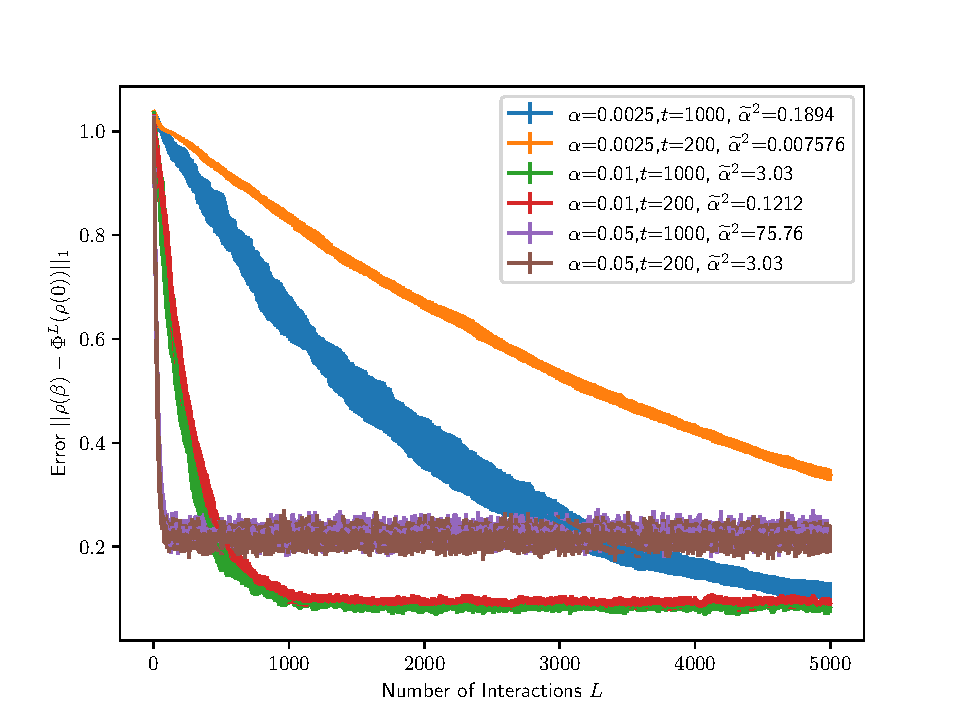
\includegraphics[width = \textwidth]{numerics/data/error_vs_interaction_h2_chain_1.pdf}    
        \caption{Hydrogen 2 }\label{fig:h2_error}
    \end{subfigure}    
    \begin{subfigure}{0.49\textwidth}
        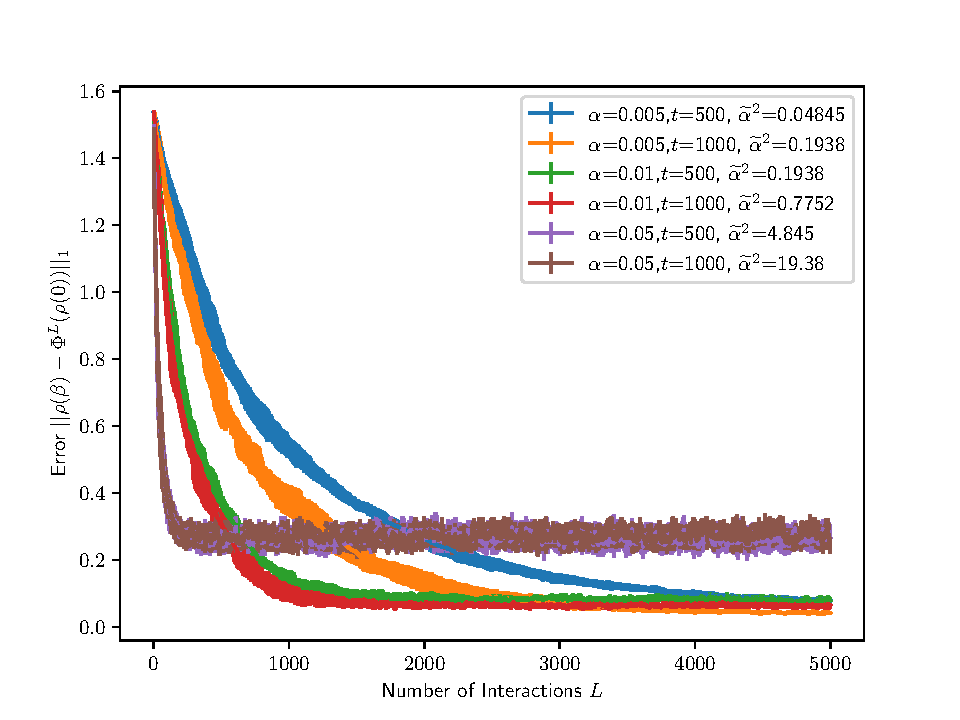
\includegraphics[width=\textwidth]{numerics/data/error_vs_interaction_h3_chain_3.pdf}
        \caption{Hydrogen 3 }\label{fig:h3_error}
    \end{subfigure} 
    \caption{These plots show the distance to the target thermal state for Hydrogen 2 and Hydrogen 3 chains as the number of interactions $L$ increases. For both Hydrogen 2 and 3 we set $\beta = 4.0$, which gives a ground state overlap of greater than 0.5 for Hydrogen 2 and 0.25 for Hydrogen 3. $\gamma$ for both \ref{fig:h2_error} and \ref{fig:h3_error} was generated by placing a Gaussian at the average energy $\trace{H_S} / \dim_S$ with a width of $\norm{H_S} / 2$. We note that a variety of $\widetilde{\alpha}^2$ values were chosen to demonstrate the faster convergence, but higher error, of strong coupling.
    }
    \label{fig:h_chain_error}
\end{figure}

There are a few key takeaways from Figure \ref{fig:h_chain_error}. The first is that we observe increasing $\alpha$ and $t$ tend to increase the convergence rate, with $\alpha$ visuallly appearing more important. At higher values of $\alpha$ changes in $t$ appear to make less of an impact on the error. We also observe that our channel is seemingly robust beyond our weak-interaction analysis. For values of $\widetilde{\alpha}^2$, the weak-interaction expansion parameter, we observe that values as high as $\widetilde{\alpha}^2 \approx 3$ can have rapid convergence to fairly low error floors. We note that these coupling values that go beyond weak-interaction seem to lead to faster convergence of the dynamics at the cost of a larger error floor. It remains an open question if dynamic choices of $\alpha$ and $t$ could lead to better performance of the overall routine, one could use very large $\widetilde{\alpha}$ initially to quickly thermalize with large error and then decrease $\widetilde{\alpha}$ to fine-tune the final state.

The second observation we make is on the choice of the environment gaps $\gamma$. For both Hydrogen 2 and 3 we selected $\gamma $ randomly from a Gaussian with mean $\trace{H_S} / \dim_S$ and standard deviation of $\norm{H_S} / 2$. This choice of $\gamma$ is completely heuristic and was intended to have a large overlap with what the typical eigenvalue differences may look like with a large enough deviation to pick up potentially large differences. Although this heuristic works well enough to show convergence, it leads us to question if the error convergence or floors can be improved with better choices of $\gamma$. 

In Figure \ref{fig:h_chain_noise} we demonstrate that better choices of $\gamma$ do in fact reduce the total simulation time needed for thermalization. In Figures \ref{fig:h2_chain_with_noise} and \ref{fig:h3_chain_with_noise} we compute the number of interactions needed at a fixed coupling constant $\alpha$ and a fixed time $t$ as a function of the noise added to our samples for $\gamma$. We generate one sample of $\gamma$ by first computing the eigenvalue spectrum of H2 or H3 exactly, then by choosing two non-equal eigenvalues, and finally sampling a Gaussian centered at the absolute value of the difference. The width of this Gaussian then serves as a proxy for the amount of knowledge one may have about the system's eigenvalues. We plot the total simulation time with respect to this width as it varies from 0 to the spectral width $\max_i \lambda_S(i) - \min_j \lambda_S(j)$. The results align well with our theoretic analysis: having knowledge of the eigenvalues of the system can be used to speed up the thermalization routine but if one does not have any knowledge at all the thermal state can still be prepared. It is an open question if the dependence of the total simulation time $L \cdot t$ on the noise level $\sigma$ can be determined analytically.
 \begin{figure}
     \centering
        \begin{subfigure}{0.49\textwidth}
        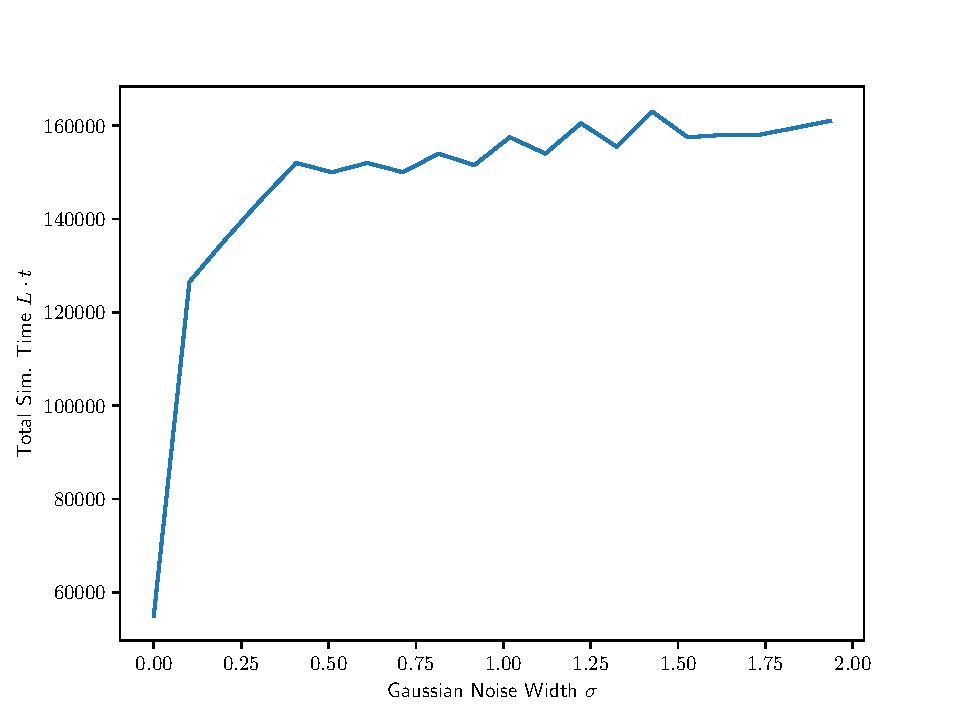
\includegraphics[width = \textwidth]{numerics/h2_chain_with_noise_3.pdf}    
        \caption{Hydrogen 2 } \label{fig:h2_chain_with_noise}
    \end{subfigure}    
    \begin{subfigure}{0.49\textwidth}
        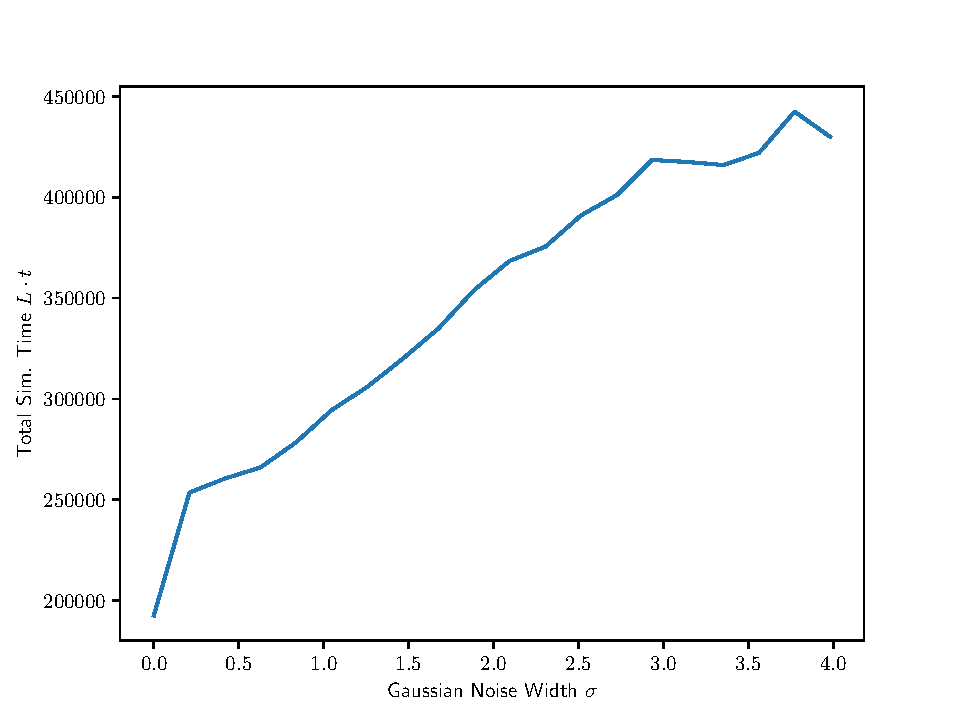
\includegraphics[width=\textwidth]{numerics/h3_chain_with_noise_3.pdf}
        \caption{Hydrogen 3 }\label{fig:h3_chain_with_noise}
    \end{subfigure} 
     \caption{ In these plots the amount of total simulation time needed to prepare a $\beta = 2.0$ thermal state with $\alpha = 0.01$ and $t = 500$ is tracked as a function of the noise added to samples of $\gamma$. A sample for $\gamma$ is generated by choosing two non-equal eigenvalues from the system spectrum and adding a Gaussian random variable with standard deviation $\sigma$. For each value of $\sigma$ the resulting state needs to have an average trace distance of less than $0.05$ for 100 samples.}
     \label{fig:h_chain_noise}
 \end{figure}




\section{Conclusion} \label{sec:conclusion}

Thermal state preparation is likely to be a crucial preparation step for the simulation of quantum systems on digital quantum computers. We have presented a thermalization routine for this task that has an optimally minimal number of overhead ancilla qubits and compiles to remarkably simple circuits of time independent Hamiltonian evolution of the unprocessed system Hamiltonian, with no filtering or rejection steps and no Fourier weighted jump operators of Linbladians. Our routine is based on relatively recent classical Monte Carlo techniques, specifically Hamiltonian Monte Carlo \cite{hoffman2011nouturnsampleradaptivelysetting} and the end result bears striking resemblance to the Repeated Interactions framework in open quantum systems \cite{prositto2025equilibrium}. In the Hamiltonian Monte Carlo algorithm thermal states over a position coordinate $q$ is prepared by sampling momentum $p$ from the Boltzmann distribution for Gaussians $e^{-\beta p^2/2m}$ followed by time evolution. Classical Hamiltonian dynamics is enough to couple the position and momentum, leading to the Boltzmann distribution over $q$ with enough time and samples. In the repeated interactions framework a quantum system interacts with many small environments, typically a single photon, that is repeated until the system thermalizes. 

Our work extends these procedures to quantum algorithms. For Hamiltonian Monte Carlo, instead of adding in momentum variables we add in a single ancilla qubit to serve as our extra state space. We do not have the luxury of classical Hamiltonian dynamics that couples these two spaces or registers, so we add in a randomized interaction term to the Hamiltonian. After simulating the time dynamics of this system-ancilla pair and repeating multiple times we are able to thermalize the system to the same $\beta$. On the other hand, the Repeated Interactions framework typically is concerned with thermodynamic limits, such as infinite time or interactions, and specific system-interactions pairs. As our procedure is intended to be used as a subroutine for quantum computers our techniques work for arbitrary, non-degenerate, Hamiltonians and purposefully use randomized interactions as opposed to a fixed interaction model.

One benefit of our thermalization procedure is that it can be compiled all the way down to the circuit level with minimal overhead in complexity. The elements of the channel that need to be compiled are: the ancilla qubit state preparation, the initial state preparation for the system, the time evolution of $H + \alpha G$, and the partial trace. The ancilla state preparation can be done starting from the ground state with a Pauli-$X$ rotation. The initial system state can be any state that commutes with $H_S$, the two leading choices are the maximally mixed state or a Haar random pure state. The maximally mixed state can be prepared using just CNOT gates at a cost of higher qubit count and a Haar random pure state can be prepared with no additional qubit overhead by applying a deep enough random circuit \cite{choi2023preparing}. 

The time evolution of $H + \alpha G$ can be broken down into simulation of $H_S$ and then $\alpha G$ by one application of Trotter. The simulation of $H_S$ can be implemented in two different ways depending on the access model for the system Hamiltonian $H_S$. If $H_S$ is provided as a block-encoding then there exist optimal simulation techniques that add only a single extra ancilla qubit \cite{low2019hamiltonian}. If $H_S$ is provided as a sum of $k$-local Pauli strings or as a sparse matrix then product formula techniques can be used \cite{childs2021theory} at zero extra overhead in ancilla qubits. To simulate the time evolution of $\alpha G$ we can use the following breakdown $e^{i \alpha G t} = e^{i \alpha U_{\haar} D U_{\haar}^\dagger t} = U_{\haar} e^{i \alpha  D  t}U_{\haar}^\dagger$. This unitary can be implemented with a 2-design to approximate the $U_{\haar}$, this is due to the fact that we only expand the channel to second order in $\alpha$. Random Clifford circuits \cite{webb2015clifford} are sufficient for this purpose. To simulate $e^{i \alpha D t}$ random $Z$ rotations and controlled-$Z$ rotations should be sufficient, as we only ever rely on the eigenvalues being pairwise independent in our analysis. In the worst case the number of random gates in the $Z$ basis that would need to be applied would scale with the dimension of the system, adding an overall factor of $\dim_S$ to the preparation. In the product formula case we further remark that $H + \alpha G$ could be simulated in total with a composite technique of using Trotter for $H$ and randomized compilation for $\alpha G$ \cite{hagan2023composite}. 

In classical Hamiltonian Monte Carlo it is well known that sharp gradients in the Hamiltonian require longer simulation time and more samples to converge. Our quantum routine has a much more subtle dependence on the structure of the Hamiltonian. As our single ancilla qubit only has one energy difference $\gamma$, we have to tune this energy difference to allow for energy to be siphoned off from the system into the ancilla. This would present a conundrum, as knowing spectral gaps is as difficult or harder than preparing ground states of arbitrary quantum Hamiltonians, but we are able to prove that our routine is robust to complete ignorance of these differences. We show that this ignorance comes at an asymptotic cost in the amount of resources needed to prepare the thermal state. We numerically verify that knowledge of the eigenvalue differences can be used to speed up the total simulation time, as demonstrated in Figure \ref{fig:h_chain_error}. We posit that this behavior serves as a crucial entry point for heuristics about Hamiltonian spectra into thermal state preparation algorithms. No prior thermal state preparation routines have had such an explicit demonstration of the utility of such knowledge. It was our hope to analytically quantify the speedups gained as a function of the relative entropy between a heuristic guess for the eigenvalue differences and the true spectra, but our numeric evidence will have to suffice until future work can clarify this dependence.

We would like to make a few remarks on potential improvements for the analysis of this channel. As we have demonstrated numerically, our guaranteed analytic values of $\alpha$ and $t$ that lead to thermalization are drastically overestimated. We conjecture that this is due to our truncation of the weak-coupling expansion and in Figure \ref{fig:epsilon_scaling} we demonstrate that taking $\alpha \propto 1/t$ and $t \propto 1/ \sqrt{\epsilon}$ drastically outperforms our analytically derived bounds of $\alpha \propto 1/t^3$, by almost 4 orders of magnitude at $\epsilon \approx 0.005$. It is an open question of how to analyze this channel in the strong-coupling regime, and our numeric results suggest that such an analysis may indicate better performance of our protocol than a weak-coupling expansion can show. It is also an open question of whether dynamically chosen values of $\alpha$ and $t$, such as having strong coupling and low time at the beginning and gradually decreasing $\alpha$ and increasing $t$, can outperform static $\alpha$ and $t$. We also suspect that the Markov relaxation theorem we used greatly overestimates the number of interactions needed. It remains to be seen if better Markov theory is needed or if the convergence time could be characterized based on the overlap of the initial state with the thermal state, which is a property that a few ground state preparation algorithms demonstrate. Another potential avenue for improving the analysis of this channel is whether different randomized interactions or even eigenvector heuristics can be beneficial. For example, in the harmonic oscillator if one has knowledge of the creation and annihilation operators $a^\dagger$ and $a$, could one simply use the interaction $a^\dagger \otimes (X + i Y) + a \otimes (X - i Y)$ instead of involving a randomized $G$ that relies on a Haar average? The last potential improvement is to extend our spectral gap computations using perturbation theory. We are only able to compute the spectral gap $\widetilde{\lambda}_\star(\beta)$ in the limit of $\beta \to \infty$, but it should be possible to compute a perturbation on the order of $1/\beta$. This would give the simulation time needed to prepare low-temperature thermal states as opposed to zero-temperature states.

Lastly, we would like to speculate on possible applications of this routine to other quantum information processing tasks. The first question that arises is if these techniques could be used in the training of quantum Boltzmann machines, which are essentially thermal states. It is an open question if our thermalizing techniques could be used to either train models or to generate output samples from an already trained model. Through the process of demonstrating that this channel prepares the system in the thermal state we have calculated the output of our channel for both the system and the environment registers, and for much larger environments than single qubits. We can turn this protocol on it's head and ask how much information about the system are these ancilla qubits carrying away with them? Preliminary explorations suggest that given knowledge about eigenvalue gaps one can use transition statistics in the ancilla qubits to infer what the inverse temperature $\beta$ is of the system, assuming the system is in a thermal state. Could this thermalizing channel instead be used to develop a Bayesian model to update beliefs about Hamiltonian spectra and system temperatures? This would represent an interaction agnostic model for performing quantum thermometry or spectroscopy, which to the best of our knowledge has not been developed yet. 

\begin{acknowledgments}
We thank Matthew Pocrnic, Alessandro Prositto, and Dvira Segal for useful discussions about repeated interaction models and Ahmet Burak Çatlı and Sophia Simon for helpful discussions on quantum thermodynamics. We thank the University of Toronto Computer Science Department for compute resources. This material is primarily based upon work supported by the U.S. Department of Energy, Office of Science, National Quantum Information Science Research Centers, Co-design Center for Quantum Advantage (C2QA) under contract number DE- SC0012704 (PNNL FWP 76274).  NW also acknowledges support from Google Inc. and Boehringer Ingelheim Inc.
\end{acknowledgments}
\bibliographystyle{unsrt}
\bibliography{bib}

\appendix 


\section{Technical Proofs} \label{sec:appendix}
\subsection{Sinc Bounds} \label{sec:appendix_sinc}

\begin{lemma}[Sinc Function Bounds] \label{lem:sinc_poly_approx}
    For $\sinc^2\left( \frac{x t}{2} \right)$ and $\delta_{\min}$ as defined in Eq. \eqref{eq:delta_min_def}, we will make significant use of the following bounds:
    \begin{align}
        |x| \ge \delta_{\min} \implies \sinc^2 \left( \frac{x t}{2} \right) &\le \frac{4}{\delta_{\min}^2 t^2} \label{eq:sinc_upper_bound} \\
        |x| \le \frac{\sqrt{2}}{t} \implies \sinc^2\left(\frac{x t}{2} \right) &\ge 1 - \frac{|x|^2 t^2}{2}. \label{eq:sinc_lower_bound}
\end{align}

\end{lemma}
\begin{proof}
    The first inequality is rather trivial
    \begin{align}
        \sinc^2 \left( \frac{x t}{2} \right) &= \frac{\sin^2 (x t /2)}{(x t / 2)^2} \le \frac{4}{x^2 t^2} \le \frac{4}{\delta_{\min}^2 t^2}.
    \end{align}
    The second involves a Taylor Series for $\sinc^2$, which we compute using the expression of $\sinc$ as $\sinc(x t/ 2) = \frac{\sin xt /2}{xt/2} = \int_0^1 \cos(sxt/2) ds$.  The first two derivatives can then be computed easily
    \begin{align}
        \frac{d \sinc^2(x t /2)}{dx} &= - t \int_0^1 \sin(sx) s ds \int_0^1 \cos(sx) ds \\
        \frac{d^2 \sinc^2(x t /2)}{dx^2} &= -t^2 / 2 \int_0^1 \cos(sx)s^2 ds \int_0^1 \cos(sx) ds + t^2 / 2 \int_0^1 \sin(sx) s ~ds \int_0^1 \sin(sx) s ~ds.
    \end{align}
    We can evaluate each of these derivatives about the origin using continuity of the derivatives along with the limits $\lim_{x \to 0} \cos(sx) = 1$ and $\lim_{x \to 0} \sin(sx) = 0$. We can now compute the mean-value version Taylor series as
    \begin{align}
        \sinc^2 \left(\frac{x t}{2} \right) &= \sinc^2(0) + x \frac{d}{dx} \sinc^2 \left(\frac{x t}{2} \right) \bigg|_{x = 0} + \frac{x^2}{2!} \frac{d^2}{dx^2} \sinc^2 \left(\frac{x t}{2} \right) \bigg|_{x = x_{\star}},
    \end{align}
    where $x_{\star} \in [0,1]$. 
    Plugging in $\sinc^2(0) = 1$ and $\frac{d\sinc^2(x t /2)}{dx}\big|_{x = 0} = 0$ then yields $|\sinc^2(xt/2) - 1| = \frac{|x|^2}{2} \abs{\frac{d^2\sinc^2(x t / 2)}{dx^2}\big|_{x = x_{\star}}}$. We make use of the rather simplistic bound
    \begin{align}
        \abs{\frac{d^2\sinc^2(sxt/2)}{dx^2}\bigg|_{x = x_{\star}} } &\leq t^2 / 2 \abs{\int_0^1 \cos(sx_{\star} t/ 2) s^2 ds \int_0^1 \cos(sx_{\star} t/ 2) ds} + t^2 /2 \abs{\int_0^1 \sin(sx_{\star} t/ 2) s ds \int_0^1 \sin(sx_{\star} t/ 2) s ds} \\
        &\leq t^2 / 2 \int_0^1 \abs{\cos(sx_{\star} t/2)} s^2 ds \int_0^1 \abs{\cos(sx_{\star} t /2 )} ds + t^2 / 2 \parens{\int_0^1 \abs{\sin(sx_{\star} t /2)} |s| ds}^2 \\
        &\leq t^2 / 2 \int_0^1 s^2 ds + t^2 / 2 \parens{\int_0^1 s ds}^2 \\
        &\leq t^2.
    \end{align}
    This yields the final inequality $|\sinc^2(x t /2 ) - 1| \leq \frac{|x|^2 t^2}{2}$ which yields Eq. \eqref{eq:sinc_lower_bound}.
\end{proof}


\subsection{Haar Integral Proofs} \label{sec:haar_integral_appendix}

In this section we present the more technical work needed to state our results in Section \ref{sec:weak_coupling}. Lemmas \ref{lem:two_heisenberg_interactions} and \ref{lem:sandwiched_interaction} are used to compute the effects of the randomized interactions in a form that are usable in the main result of Lemma \ref{lem:big_one}. Lemma \ref{lem:haar_two_moment} can be derived from Appendix C in \cite{brandao2021complexity}.
\begin{restatable}{lemma}{haar_two_moment} \label{lem:haar_two_moment}
    Let $\int (\cdot) dU$ denote the average distributed according to the Haar measure over $\dim$-dimensional unitary matrices $U$. Then for $\ket{i_1},\ket{i_2},\ldots,\ket{k_2}$ drawn from an orthonormal basis
    \begin{align}
        &\int \bra{i_1} U \ket{j_1} \bra{i_2} U \ket{j_2} \bra{k_1} U^\dagger \ket{l_1} ~ \bra{k_2} U^\dagger \ket{l_2} dU \nonumber \\
        &= ~\frac{1}{\dim^2 - 1} \parens{\delta_{i_1, l_1} \delta_{j_1, k_1} \delta_{i_2, l_2} \delta_{j_2, k_2} + \delta_{i_1, l_2} \delta_{j_1, k_2} \delta_{i_2, l_1} \delta_{j_2, k_1}} \nonumber \\
        &\quad - \frac{1}{\dim(\dim^2 - 1)} \parens{\delta_{i_1, l_2} \delta_{j_1, k_1} \delta_{i_2, l_1} \delta_{j_2, k_2} + \delta_{i_1, l_1} \delta_{j_1, k_2} \delta_{i_2, l_2} \delta_{j_2, k_1}}. \label{eq:haar_two_moment_integral}
    \end{align}
\end{restatable}

\begin{lemma} \label{lem:two_heisenberg_interactions}
    Let $G(t)$ denote the Heisenberg evolved random interaction $G(t) = e^{iHt} G e^{-iHt}$ for a total Hamiltonian $H$. After averaging over the interaction measure the product $G(x) G(y)$ can be computed as
    \begin{equation}
        \int G(x) G(y) dG = \frac{1}{\dim + 1} \parens{\sum_{(i,j),(k,l)} e^{i \Delta(i,j|k,l) (x-y)} \ketbra{i,j}{i,j} + \identity}.
    \end{equation}
\end{lemma}
\begin{proof}
The overall structure of this proof is to evaluate the product in the Hamiltonian eigenbasis and split the product into three factors: a phase contribution from the time evolution, a Haar integral from the eigenvalues of the random interaction, and the eigenvalue contribution of the random interaction. Since this involves the use of multiple indices, it will greatly simplify the proof to use a single index over the total Hilbert space $\hilb$ as opposed to two indices over $\hilb_S \otimes \hilb_E$. For example, the index $a$ should be thought of as a pair $(a_s, a_e)$, and functions $\lambda(a)$ should be thought of as $\lambda(a_s, a_e)$. Once the final form of the expression is reached we will substitute in pairs of indices for easier use of the lemma in other places.
    \begin{align}
        \int G(x) G(y) dG &= \int e^{+i H x} U_G D U_G^\dagger e^{-i H x} e^{+i H y} U_G D U_G^\dagger e^{-i H y} dU_G ~dD \\
        &= \int \bigg[\sum_a e^{+i \lambda(a)x}\ketbra{a}{a}  U_G \sum_b D(b)\ketbra{b}{b} U_G^\dagger \nonumber \\
        &\quad \sum_c e^{-i \lambda(c) (x - y)} \ketbra{c}{c} U_G \sum_d D(d)\ketbra{d}{d} U_G^\dagger \sum_e e^{-i \lambda(e) y} \ketbra{e}{e} \bigg] dU_G ~dD\\
        &=\sum_{a,b,c,d,e} \ketbra{a}{e} e^{-i (\lambda(c) - \lambda(a))x} e^{-i (\lambda(e) - \lambda(c))y} \nonumber \\
        &\quad \times \int \bra{a} U_G \ket{b} \bra{c} U_G \ket{d} \bra{b} U_G^{\dagger} \ket{c} \bra{d} U_G^\dagger \ket{e} dU_G \int D(b) D(d) dD \\
        &=  \sum_{a, b, c, d, e} \delta_{bd} \ketbra{a}{e} e^{-i (\lambda(c) - \lambda(a))x} e^{-i (\lambda(e) - \lambda(c))y} \nonumber \\
        &\quad \times \int \bra{a} U_G \ket{b} \bra{c} U_G \ket{d} \bra{b} U_G^{\dagger} \ket{c} \bra{d} U_G^\dagger \ket{e} dU_G. \\
    \end{align}
    Now the summation over $d$ fixes $d=b$ and we use Lemma \ref{lem:haar_two_moment} to compute the Haar integral, which simplifies greatly due to the repeated $b$ index. Plugging the result into the above yields the following
    \begin{align}
        &= \frac{1}{\dim^2 - 1} \sum_{a, b, c, e} \ketbra{a}{e} e^{-i (\lambda(c) - \lambda(a))x} e^{-i (\lambda(e) - \lambda(c))y} \parens{\delta_{ac} \delta_{ce} + \delta_{ae} - \frac{1}{\dim} \parens{\delta_{ac} \delta_{ce} + \delta_{ae}}}  \\
        &= \frac{1}{\dim^2 - 1} \parens{1 - \frac{1}{\dim}} \sum_{a, b, c, e} \ketbra{a}{e} e^{-i (\lambda(c) - \lambda(a))x} e^{-i (\lambda(e) - \lambda(c))y} \delta_{ae} (1 + \delta_{ac}) \\
        &= \frac{1}{\dim^2 - 1} \parens{1 - \frac{1}{\dim}} \sum_{a, b, c} \ketbra{a}{a} e^{i (\lambda(a) - \lambda(c))(x-y)} (1 + \delta_{ac}) \\
        &= \frac{1 \parens{\dim - 1}}{\dim^2 - 1} \sum_{a,c} \ketbra{a}{a} e^{i (\lambda(a) - \lambda(c))(x - y)} (1 + \delta_{ac}) \\
        &= \frac{1}{\dim + 1} \parens{\sum_{a,c} e^{i (\lambda(a) - \lambda(c))(x-y)} \ketbra{a}{a} + \identity}.
    \end{align}
    Reindexing by $a \mapsto i,j$, $c \mapsto k,l$, and plugging in the definition of $\Delta$ yields the statement of the lemma.
\end{proof}


\begin{lemma} \label{lem:sandwiched_interaction}
    Given two Heisenberg evolved random interactions, $G(x)$ and $G(y)$, we compute their action on an outer-product $\ketbra{i,j}{k,l}$ as
    \begin{equation}
        \int G(x) \ketbra{i,j}{k,l} G(y) ~dG = \frac{1}{\dim + 1} \parens{\ketbra{i,j}{k,l} + \braket{i,j}{k,l} \sum_{m,n} e^{i \Delta(m,n | i,j) (x-y)} \ketbra{m,n}{m,n}}
    \end{equation}
\end{lemma}
\begin{proof}
This proof is structured the same as Lemma \ref{lem:two_heisenberg_interactions} and similarly we will use a single index of the total Hilbert space $\hilb$ and switch to two indices to match the rest of the exposition.
    \begin{align}
        \int G(x) \ketbra{a}{b} G(y) dG &=  \int e^{i H x} U_G D U_G^{\dagger} e^{-i H x} \ketbra{a}{b} e^{i H y} U_G D U_G^\dagger e^{-i H y} ~dG \\
        &= \sum_{c, d, e, f} e^{i (\lambda(c) - \lambda(a))x} e^{i (\lambda(b) - \lambda(f))y} \nonumber \\
        &\quad \times \int \ketbra{c}{c} U_G D(d) \ketbra{d}{d} U_G^\dagger \ketbra{a}{b} U_G D(e) \ketbra{e}{e} U_G^\dagger \ketbra{f}{f} dG \\
        &= \sum_{c, d, e, f}  e^{i (\lambda(c) - \lambda(a))x} e^{i (\lambda(b) - \lambda(f))y} \ketbra{c}{f} \nonumber \\
        &\quad \times \int D(d) D(e) dD \int \bra{c} U_G \ket{d} \bra{b} U_G \ket{e} \bra{d} U_G^\dagger \ket{a} \bra{e} U_G^\dagger \ket{f} dU_G \\
        &=  \sum_{c,d,f} e^{i (\lambda(c) - \lambda(a))x} e^{i (\lambda(b) - \lambda(f))y} \ketbra{c}{f} \nonumber \\ 
        &\quad \times \int \bra{c} U_G \ket{d} \bra{b} U_G \ket{d} \bra{a} \overline{U_G} \ket{d} \bra{f} \overline{U_G} \ket{d} dU_G \\
        &= \frac{1}{\dim^2 - 1} \sum_{c,d,f} e^{i (\lambda(c) - \lambda(a))x} e^{i (\lambda(b) - \lambda(f))y} \ketbra{c}{f} (\delta_{ca} \delta_{bf} + \delta_{cf}\delta_{ab})\parens{1 - \frac{1}{\dim}} \\
        &= \frac{1}{\dim + 1} \sum_{c,f} e^{i (\lambda(c) - \lambda(a))x} e^{i (\lambda(b) - \lambda(f))y} \ketbra{c}{f} (\delta_{ca} \delta_{bf} + \delta_{cf}\delta_{ab}) \\
        &= \frac{1}{\dim + 1} \parens{\ketbra{a}{b} + \delta_{ab} \sum_{c} e^{i(\lambda(c) - \lambda(a))(x-y)} \ketbra{c}{c} }.
    \end{align}
    Now re-indexing by $a \mapsto (i,j)$, $b \mapsto (k,l)$ and $c \mapsto (m,n)$ results in the expression given in the statement of the lemma.
\end{proof}


\secondOrderChannelHaar*
\begin{proof}
To start we would like to note that we will use a single index notation to refer to the joint system-environment eigenbasis during this proof to help shorten the already lengthy expressions. We will convert back to a double index notation to match the statement of the theorem. We start from the expression for the first derivative of the channel $\frac{\partial}{\partial \alpha} \Phi_G(\rho_S)$ given by Eq. \eqref{eq:first_order_alpha_derivative}. To take the second derivative there are six factors involving $\alpha$, so we will end up with six terms. We repeat Eq. \eqref{eq:first_order_alpha_derivative} below, add a derivative, and label each factor containing an $\alpha$ for easier computation
\begin{align}
    \frac{\partial^2}{\partial \alpha^2} \Phi_G(\rho_S) =& \frac{\partial}{\partial \alpha} \parens{\int_{0}^{1} \underset{\substack{\downarrow \\ (A)}}{e^{i s (H+\alpha G)t}} (i t G) \underset{\substack{\downarrow \\ (B)}}{e^{i (1-s) (H+\alpha G)t}} ds ~ \rho \underset{\substack{\downarrow \\ (C)}}{e^{-i(H+\alpha G)t}} } \nonumber \\
    &~ ~+\frac{\partial}{\partial \alpha} \parens{ \underset{\substack{\downarrow \\ (D)} }{e^{i(H+\alpha G)t}} \rho \int_{0}^1 \underset{\substack{\downarrow \\ (E)} }{e^{-i s (H+\alpha G) t} } (- i t G) \underset{\substack{\downarrow \\ (F)}}{e^{-i (1-s) (H+\alpha G)t}} ds }. \label{eq:second_derivative_labels}
\end{align}
Our goal is to get each of these terms in a form in which we can use either Lemma \ref{lem:two_heisenberg_interactions} or \ref{lem:sandwiched_interaction}. 
\begin{align}
    (A) &=i t\int_0^1 \parens{\frac{\partial}{\partial \alpha} e^{i s_1 (H+ \alpha G)t}} G e^{i(1-s_1)(H+\alpha G)t} ds_1 \rho e^{-i (H+\alpha G)t} \bigg|_{\alpha=0} \\
    &= (it)^2 \int_0^1 \parens{\int_0^1 e^{i s_1 s_2 (H+\alpha G)t} s_1 G e^{i s_1 (1-s_2) (H+\alpha G)t} ds_2} G e^{i(1-s_1) (H+\alpha G)t} ds_1 \rho e^{-i(H+\alpha G) t} \bigg|_{\alpha=0} \label{eq:second_order_deriv_intermediate_a}\\
    &= -t^2 \int_0^1 \int_0^1 e^{i s_1 s_2 H t} G e^{-i s_1 s_2 H t} e^{i s_1 H t} G e^{-i s_1 H t} s_1 ds_1 ds_2 e^{i H t} \rho e^{-i H t} \\
    &= -t^2 \int_0^1 \int_0^1 G(s_1 s_2 t) G(s_1 t) s_1 ds_1 ds_2 \rho(t). \label{eq:second_deriv_alpha_first_term}
\end{align}

\begin{align}
    (B) &= it \int_0^1 e^{i s_1 (H + \alpha G)t} G \frac{\partial}{\partial \alpha}\parens{e^{i(1-s_1)(H + \alpha G)t}} ds_1 \rho e^{-i(H + \alpha G) t} \bigg|_{\alpha = 0} \\
    &= (it)^2 \int_0^1 e^{i s_1 (H + \alpha G)t} G \parens{\int_0^1 e^{i(1-s_1)s_2 (H + \alpha G)t} (1-s_1) G e^{i(1 - s_1)(1 - s_2)(H + \alpha G)t} ds_2} ds_1 ~ \rho e^{-i ( H + \alpha G)t} \bigg|_{\alpha = 0} \\
    &= -t^2 \int_0^1 \int_0^1 e^{i s_1 H t} G e^{i(1-s_1)s_2 H t} G e^{i(1-s_1)(1-s_2) H t} (1-s_1) ds_1 ds_2 ~ \rho e^{-i H t}\\ 
    &= -t^2 \int_0^1 \int_0^1 e^{i s_1 H t} G e^{-i s_1 H t} e^{i(s_1 + s_2 - s_1 s_2) H t} G e^{-i (s_1 + s_2 - s_1 s_2) H t} (1-s_1) ds_1 ds_2 ~ \rho(t) \\
    &= -t^2 \int_0^1 \int_0^1 G(s_1 t) G((s_1 + s_2 - s_1 s_2)t) (1-s_1) ds_1 ds_2 ~ \rho(t)
\end{align}

\begin{align}
    (C) &= it \int_0^1 e^{i s (H + \alpha G)t} G e^{i(1-s) (H + \alpha G) t} ds ~\rho ~ \frac{\partial}{\partial \alpha} \parens{ e^{-i (H + \alpha G) t} } \bigg|_{\alpha = 0} \\
    &= (i t) (-it) \int_0^1 e^{i s (H + \alpha G)t} G e^{i (1 - s) (H + \alpha G)t} ds ~ \rho ~ \parens{ \int_0^1 e^{-i s (H + \alpha G)t} G e^{-i (1- s) ( H + \alpha G)t } ds}\bigg|_{\alpha = 0} \\
    &= + t^2 \parens{\int_0^1 e^{i s H t} G e^{-i s H t} ds} e^{i H t} \rho e^{-i H t} \parens{\int_0^1 e^{i (1-s) H t} G e^{-i (1-s) H t} ds} \\
    &= + t^2 \int_0^1 G(st) ds ~ \rho(t) \int_0^1 G((1-s)t) ds
\end{align}

\begin{align}
    (D) &= (-it) \frac{\partial}{\partial \alpha} \parens{e^{i(H + \alpha G)t}} \rho \int_0^1 e^{-i s (H + \alpha G)t} G e^{-i (1-s)(H + \alpha G)t} ds \bigg|_{\alpha = 0} \\
    &= t^2 \parens{\int_0^1 e^{i s (H+ \alpha G)t} G e^{i (1-s) (H + \alpha G)t}ds} \rho \int_0^1 e^{-i s (H + \alpha G)t} G e^{-i (1-s)(H + \alpha G)t} ds \bigg|_{\alpha = 0} \\
    &=  t^2 \int_0^1 e^{i s H t} G e^{-i s H t} ds ~\rho(t) \int_0^1 e^{i (1-s) H t} G e^{-i (1-s) H t} ds \\
    &= t^2 \int_0^1 G(st) ds ~ \rho(t) ~ \int_0^1 G((1-s)t) ds
\end{align}

\begin{align}
    (E) &= (-it) e^{i (H+ \alpha G) t} ~ \rho ~\int_0^1 \frac{\partial}{\partial \alpha} \parens{e^{-i s_1 (H + \alpha G)t}} G e^{-i (1-s_1)(H + \alpha G)t} ds_1 \bigg|_{\alpha = 0} \\
    &= - t^2 e^{i(H + \alpha G)t} ~ \rho ~\int_0^1 \parens{\int_0^1 e^{-i s_1 s_2 (H + \alpha G) t} (s_1 G) e^{-i s_1 (1-s_2) (H + \alpha G)t} ds_2} G e^{-i(1-s_1)(H + \alpha G)t} ds_1 \bigg|_{\alpha = 0} \\
    &= -t^2 e^{i H t} \rho e^{-i H t} \int_0^1 \int_0^1 e^{i (1 - s_1 s_2) H t} G e^{-i (s_1 - s_1 s_2)H t} G e^{-i (1-s_1)H t} s_1 ds_1 ds_2 \\
    &= -t^2 \rho(t) \int_0^1 \int_0^1 G((1- s_1 s_2) t) G((1-s_1)t) s_1 ds_1 ds_2
\end{align}

\begin{align}
    (F) &= (-it) e^{i(H + \alpha G) t} \rho \int_0^1 e^{-i s_1 ( H + \alpha G) t} G \frac{\partial}{\partial \alpha} \parens{ e^{-i (1-s_1) ( H +\alpha G)t}} ds_1 \bigg|_{\alpha = 0} \\
    &= (-it)^2 e^{i (H + \alpha G)t} \rho \int_0^1 e^{-i s_1 (H + \alpha G)t} G \parens{\int_0^1 e^{-i(1-s_1) s_2 (H + \alpha G)t} (1-s_1) G e^{-i(1-s_1) (1-s_2) (H + \alpha G) t} ds_2} ds_1 \bigg|_{\alpha = 0} \\
    &= -t^2 e^{-i H t} \rho e^{-i H t} \int_0^1 \int_0^1 e^{i (1- s_1) H t} G e^{-i (1-s_1) H t} e^{i (1-s_1)(1-s_2) H t} G e^{-i(1-s_1)(1-s_2) H t} (1-s_1) ds_1 ds_2 \\
    &= -t^2 \rho(t) \int_0^1 \int_0^1 G((1-s_1)t) G((1-s_1)(1 - s_2) t) (1-s_1)ds_1 ds_2
\end{align}

Now our goal is to compute the effects of averaging over the interaction $G$ on the above terms, starting with $(A)$. As this involves a lot of index manipulations, similarly to the proofs of Lemmas \ref{lem:two_heisenberg_interactions} and \ref{lem:sandwiched_interaction} we will use a single index for the total system-environment Hilbert space and switch back to a double index to state the results. We will make heavy use of Lemma \ref{lem:two_heisenberg_interactions}.
\begin{align}
    \int (A) dG &= -t^2 \int_0^1 \int_0^1 \int G(s_1 s_2 t) G(s_1 t) dG s_1 ds_1 ds_2 \rho(t) \\
    &= \frac{-t^2 }{\dim + 1} \int_0^1 \int_0^1 \parens{\sum_{i,j} e^{i (\lambda(i) - \lambda(j)) (s_1 s_2 t - s_1 t)} \ketbra{i}{i} + \identity} s_1 ds_1 ds_2 \rho(t) \\
    &= \frac{- t^2 }{\dim + 1} \parens{\sum_{i} \sum_{j : \lambda(i) \neq \lambda(j)} \int_0^1 \int_0^1 e^{i(\lambda(i) - \lambda(j))t (s_1 s_2 - s_1)} s_1 ds_1 ds_2 \ketbra{i}{i} + \sum_{i} \sum_{j : \lambda(i) = \lambda(j)}\frac{1}{2} \ketbra{i}{i} + \frac{1}{2} \identity} \rho(t) \\
    &= \frac{- t^2 }{\dim + 1} \parens{\sum_i \sum_{j : \lambda(i) \neq \lambda(j)} \frac{1 - i (\lambda(i) - \lambda(j))t - e^{-i (\lambda(i) - \lambda(j))t}}{t^2 (\lambda(i) - \lambda(j))^2} \ketbra{i}{i} + \frac{1}{2} \sum_{i} (\eta(i) + 1) \ketbra{i}{i} } \rho(t) \\
    &= \frac{- 1}{\dim + 1}\parens{\sum_{i} \sum_{j: \Delta_{ij} \neq 0} \frac{1 - i \Delta_{ij}t - e^{-i \Delta_{ij} t}}{\Delta_{ij}^2} \ketbra{i}{i} + \frac{t^2}{2} \sum_{i} (\eta(i) + 1)\ketbra{i}{i} } \rho(t)
\end{align}

We can similarly compute the averaged $(B)$ term:
\begin{align}
    \int (B) dG &= -t^2 \int_0^1 \int_0^1 \int G(s_1 t) G((s_1 + s_2 - s_1 s_2) t) dG (1-s_1) ds_1 ds_2 ~ \rho(t) \\
    &= \frac{- t^2 }{\dim + 1} \int_0^1 \int_0^1 \parens{\sum_{i,j} e^{i (\lambda(i) - \lambda(j))(s_1 s_2 - s_2) t} \ketbra{i}{i} + \identity} (1 -s_1) ds_1 ds_2 \rho \\
    &= \frac{- t^2 }{\dim + 1} \parens{\sum_{i} \sum_{j : \lambda(i) \neq \lambda(j)} \int_0^1 \int_0^1 e^{i(\lambda(i) - \lambda(j))t (s_1 s_2 - s_2)} (1 - s_1) ds_1 ds_2 \ketbra{i}{i} + \sum_{i} \sum_{j : \lambda(i) = \lambda(j)}\frac{1}{2} \ketbra{i}{i} + \frac{1}{2} \identity} \rho(t) \\
    &= \frac{- t^2 }{\dim + 1} \parens{\sum_i \sum_{j : \lambda(i) \neq \lambda(j)} \frac{1 - i (\lambda(i) - \lambda(j))t - e^{-i (\lambda(i) - \lambda(j))t}}{t^2 (\lambda(i) - \lambda(j))^2} \ketbra{i}{i} + \frac{1}{2} \sum_{i} (\eta(i) + 1) \ketbra{i}{i} } \rho(t) \\
    &= \frac{-1}{\dim + 1}\parens{\sum_{i} \sum_{j: \Delta_{ij} \neq 0} \frac{1 - i \Delta_{ij}t - e^{-i \Delta_{ij} t}}{\Delta_{ij}^2} \ketbra{i}{i} + \frac{t^2}{2} \sum_{i} (\eta(i) + 1)\ketbra{i}{i} } \rho(t),
\end{align}
which we note is identical to $\int (A) dG$. As terms $(C)$ and $(D)$ involve a different method of computation we skip them for now and compute $(E)$ and $(F)$. 
\begin{align}
    \int (E) dG &= -t^2 \rho(t) \int_0^1 \int_0^1 \int G((1- s_1 s_2) t) G((1-s_1)t) dG s_1 ds_1 ds_2 \\
    &= \frac{- t^2}{\dim + 1} \rho(t) \int_0^1 \int_0^1 \parens{\sum_{i,j} e^{i(\lambda(i) - \lambda(j)) t (s_1 - s_1 s_2)} \ketbra{i}{i} + \identity } s_1 ds_1 ds_2 \\
    &= \frac{- t^2}{\dim + 1} \rho(t) \parens{\sum_i \sum_{j : \lambda(i) \neq \lambda(j)} \frac{1 + i (\lambda(i) - \lambda(j))t - e^{i(\lambda(i) - \lambda(j))t}}{t^2 (\lambda(i) - \lambda(j))^2}\ketbra{i}{i} + \frac{1}{2} \sum_{i} (\eta(i) + 1 )\ketbra{i}{i}} \\
    &= \frac{- 1}{\dim + 1} \rho(t) \parens{\sum_i \sum_{j: (\Delta_{ij} \neq 0)} \frac{1 + i \Delta_{ij}t - e^{i\Delta_{ij}t}}{\Delta_{ij}^2} \ketbra{i}{i} + \frac{t^2}{2}\sum_i (\eta(i) + 1) \ketbra{i}{i}}.
\end{align}
Computing $(F)$ yields
\begin{align}
    \int (F) dG &= -t^2 \rho(t) \int_0^1 \int_0^1 \int G((1-s_1)t) G((1-s_1)(1 - s_2) t) dG (1-s_1)ds_1 ds_2 \\
    &= \frac{- t^2 \sigma ^2}{\dim + 1} \rho(t) \int_0^1 \int_0^1 \parens{\sum_{i,j} e^{i(\lambda(i) - \lambda(j))t (s_2 - s_1 s_2)}\ketbra{i}{i} + \identity} (1-s_1) ds_1 ds_2 \\
    &= \frac{- t^2 }{\dim + 1} \rho(t) \parens{\sum_{i} \sum_{j : \lambda(i) \neq \lambda(j)} \frac{1 + i (\lambda(i) - \lambda(j))t - e^{i (\lambda(i) - \lambda(j))t}}{t^2 (\lambda(i) - \lambda(j))^2} \ketbra{i}{i} +\frac{1}{2} \sum_{i} (\eta(i) + 1) \ketbra{i}{i}} \\
    &= \frac{- 1}{\dim + 1} \rho(t) \parens{\sum_i \sum_{j: (\Delta_{ij} \neq 0)} \frac{1 + i \Delta_{ij}t - e^{i\Delta_{ij}t}}{\Delta_{ij}^2} \ketbra{i}{i} + \frac{t^2}{2}\sum_i (\eta(i) + 1) \ketbra{i}{i}}
\end{align}
 which is identical to $\int (E) dG$.

 The last two terms $(C) = (D)$ are computed as follows:
 \begin{align}
     \int (C) dG &= t^2 \int_0^1 \int_0^1 \int G(s_1 t) \rho(t) G((1-s_2)t) ~dG ~ ds_1 ds_2 \\
     &= t^2 \sum_{i,j} \rho_{ij} e^{i(\lambda(i) - \lambda(j))t} \int_0^1 \int_0^1 \int G(s_1 t) \ketbra{i}{j} G((1-s_2)t) ~ dG ~ ds_1 ds_2 \\
     &= \frac{ t^2}{\dim + 1} \sum_{i,j} \rho_{ij} e^{i(\lambda(i) - \lambda(j))t} \parens{ \ketbra{i}{j} + \delta_{ij} \sum_{a} \int_0^1 \int_0^1 e^{i(\lambda(a) - \lambda(i))(s_1 + s_2 - 1)t} ds_1 ds_2 \ketbra{a}{a}} \\
     &= \frac{ t^2}{\dim + 1} \sum_{i,j} \rho_{ij} e^{i \Delta_{ij} t} \parens{\ketbra{i}{j} + \delta_{ij} \sum_{a : \Delta_{ai} \neq 0} \frac{2( 1- \cos (\Delta_{ai} t))}{\Delta_{ai}^2 t^2} \ketbra{a}{a} + \delta_{ij} \sum_{a : \Delta_{ai} = 0} \ketbra{a}{a}}
 \end{align}

 We can now combine each of these terms to offer the full picture of the output of the channel to second order. We make two modifications to the results from each sum: first, we will switch to double index notation to make for easier use in other areas, and secondly we let $\rho = \ketbra{i,j}{k,l}$. We note that the first term in the following equation is provided by $(A) + (B)$, the second through $(E) + (F)$, and the last two through $(C) + (D)$. 
 \begin{align}
     &\int \frac{\partial^2}{\partial \alpha^2} \Phi_G(\ketbra{i,j}{k,l})\bigg|_{\alpha = 0} dG \\
     &= -\frac{2  e^{i \Delta(i,j|k,l) t}}{\dim + 1} \bigg(\sum_{(a,b): \Delta(i,j|a,b) \neq 0} \frac{1 - i \Delta(i,j|a,b)t - e^{-i \Delta(i,j|a,b) t}}{\Delta(i,j|a,b)^2} \nonumber \\
     &~+ \sum_{(a,b): \Delta(k,l|a,b) \neq 0} \frac{1 + i \Delta(k,l|a,b) t - e^{i \Delta(k,l|a,b) t}}{\Delta(k,l|a,b)^2} + \frac{t^2}{2}(\eta(i,j) + \eta(k,l)) \bigg) \ketbra{i,j}{k,l} \nonumber \\
    &~ +\delta_{i,k} \delta_{j,l} \frac{2 e^{i \Delta(i,j|k,l)t}}{\dim+1} \parens{ \sum_{(a,b): \Delta(i,j|a,b) \neq 0 } \frac{2(1- \cos (\Delta(i,j|a,b)t))}{\Delta(i,j|a,b)^2} \ketbra{a,b}{a,b} + t^2 \sum_{(a,b) : \Delta(i,j|a,b) = 0} \ketbra{a,b}{a,b}} \label{eq:second_order_output}
 \end{align}
The last step we need is to use the half angle formula to change the cosine to a sine
\begin{align}
    \frac{2(1 - \cos(\Delta(i,j| a,b)t)}{\Delta(i,j|a,b)^2} &= \frac{2\left( 1 - \left(1 - 2 \sin^2\left(\frac{\Delta(i,j|a,b)t}{2} \right) \right) \right)}{\Delta(i,j|a,b)^2} \label{eq:trig_start} \\
    &= t^2 \frac{\sin^2 \left(\frac{\Delta(i,j|a,b) t}{2} \right)}{\frac{\Delta(i,j|a,b)^2 t^2}{4}} \\
    &= t^2 \sinc^2 \left(\frac{\Delta(i,j|a,b) t}{2 } \right), \label{eq:trig_end}
\end{align}
which yields the statement.


We can compute these by plugging in to Eq. \eqref{eq:el_gigante} again, which yields
\begin{align}s
&\int \bra{i', j'} \mathcal{T} \left( \ketbra{i, j}{i, j} \right) \ket{i', j'} ~dG = \begin{cases}        
\widetilde{\alpha}^2 \sinc^2(\Delta(i,j | i', j') t /2) & (i, j) \neq (i', j') \\
            - \widetilde{\alpha}^2 \sum_{(a,b) \neq (i, j)} \sinc^2(\Delta(a,b|i,j) t / 2) & (i,j) = (i', j')
        \end{cases}. \label{eq:system_environment_transitions}
    \end{align}
    The $(i, j) \neq (i', j')$ case should be apparent, the first term with the coherence factors $\chi$ are zero and the second term is what remains. The $(i,j) = (i', j')$ case can be seen as follows. For the first term we have
    \begin{align}
        - \frac{\alpha^2 e^{i \Delta(i,j| i,j) t}}{\dim + 1}\left(\chi(i,j) + \chi(i,j)^* + \frac{t^2}{2}(\eta(i,j) + \eta(i,j) \right) \ketbra{i,j}{i,j}.
    \end{align}
    We first compute the sum $\chi(i,j) + \chi(i,j)^*$ as
    \begin{align}
        \chi(i,j) + \chi(i,j)^* &= \sum_{a,b: \Delta(i,j,|a,b) \neq 0} \frac{1 - i \Delta(i,j|a,b)t - e^{-i \Delta(i,j|a,b) t}}{\Delta(i,j|a,b)^2} \nonumber\\
&\quad+ \sum_{a,b: \Delta(i,j,|a,b) \neq 0} \frac{1 + i \Delta(i,j|a,b)t - e^{+i \Delta(i,j|a,b) t}}{\Delta(i,j|a,b)^2} \\
    &= \sum_{a,b: \Delta(i,j| a,b) \neq 0} \frac{2 - e^{-i \Delta(i,j| a,b) t} - e^{+i \Delta(i,j| a,b) t}}{\Delta(i,j|a,b)^2} \\
    &= \sum_{a,b: \Delta(i,j| a,b) \neq 0} t^2 \sinc^2 \left( \frac{\Delta(i,j| a,b) t}{2} \right),
    \end{align}
    where the last step follows from a trigonometric identity (see Eqs. \eqref{eq:trig_start} - \eqref{eq:trig_end} in Appendix \ref{sec:haar_integral_appendix} for details). Since $\sinc(0) = 1$ the $\eta(i,j)$ term can be expressed as $\eta(i,j) = \sum_{a,b : \Delta(i,j|a,b) = 0} \sinc^2 \left( \frac{\Delta(i,j| a,b) t}{2} \right)$. Plugging this into Eq. \eqref{eq:el_gigante} gives
    \begin{align}
        &\int \bra{i,j} \mathcal{T} (\ketbra{i,j}{i,j}) \ket{i,j} dG \\
        &= \bra{i,j} \left(-\frac{\alpha^2 t^2}{\dim + 1} \sum_{a,b} \sinc^2 \left( \frac{\Delta(i,j| a,b) t}{2} \right) \ketbra{i,j}{i,j} + \sum_{a,b} \sinc^2\left( \frac{\Delta(i,j | a,b)t}{2} \right) \ketbra{a,b}{a,b} \right) \ket{i,j} \\
        &= -\frac{\alpha^2 t^2}{\dim + 1} \sum_{(a,b) \neq (i,j)} \sinc^2 \left( \frac{\Delta(i,j| a,b) t}{2} \right).
    \end{align}
    As a by-product of this computation we have just shown that $\trace{\mathcal{T}(\rho)} = 0$ and that our mapping is trace preserving to $\bigo{\alpha^2}$.
\end{proof}

\subsection{Weak-Coupling Remainder Bound} \label{sec:weak_coupling_remainder_bound}

\begin{proof}[Proof of Theorem~\ref{thm:remainder_bound}]
First we note that although $R_{\Phi}(\rho) = \frac{\alpha^3}{6} \partial_{\alpha}^3 \Phi(\rho)\big|_{\alpha = \alpha_{\star}}$ for a specific $ \alpha_{\star} > 0$ our proof will hold for any $\alpha_{\star}$. To compute the trace norm we will use the triangle inequality, unitary invariance of the Sch\"{a}tten norms, and submultiplicativity. To start,
\begin{align}
    \|\partial_\alpha^3 \Phi(\rho) \|_1 &= \left\| \frac{\partial^3}{\partial \alpha^3} {\rm Tr}_{H_E} \int e^{i(H+\alpha G)t} \rho_S \otimes \rho_E e^{-i(H+\alpha G)t} dG \bigg|_{\alpha = \alpha_{\star}} \right\|_1 \nonumber\\
    &= \left\| \frac{\partial^3}{\partial \alpha^3} {\rm Tr}_{H_E} \int e^{i(H+\alpha G)t} \rho_S \otimes \rho_E e^{-i(H+\alpha G)t} dG \bigg|_{\alpha = \alpha_{\star}} \right\|_1 \nonumber\\
    &\le    \int \left\|{\rm Tr}_{H_E}\frac{\partial^3}{\partial \alpha^3}\left( e^{i(H+\alpha G)t} \rho_S \otimes \rho_E e^{-i(H+\alpha G)t}\right) \bigg|_{\alpha = \alpha_{\star}} \right\|_1 dG.\label{eq:3derivBd}
\end{align}
To proceed, Proposition 1 of \cite{rastegin2012relations} allows us to eliminate the partial trace using the relation
$\norm{\partrace{\hilb_E}{X}}_{1} \le \norm{X}_{\dim_E} \le \norm{X}_1$. Further we use the decomposition of the second derivatives from the proof of Lemma \ref{lem:big_one}, specifically  Eq. \eqref{eq:second_derivative_labels} for the definition of each term, as $\partial_{\alpha}^2 \Phi_G = (A) + (B) + (C) + (D) +(E) + (F)$. This gives the following 
\begin{align}
    \norm{R_{\Phi}}_1 \le \frac{\alpha^3}{6} &\int \norm{\partial_{\alpha}((A) + (B) + (C) + (D) +(E) + (F)) \big|_{\alpha = \alpha_{\star}} }_1 dG \\
    &\le \frac{\alpha^3}{6} \int \norm{\partial_{\alpha}(A)\big|_{\alpha = \alpha_{\star}} }_1 + \norm{\partial_{\alpha}(B) \big|_{\alpha = \alpha_{\star}} }_1 + \ldots + \norm{\partial_{\alpha}(F) \big|_{\alpha = \alpha_{\star}} }_1 dG
\end{align}
We will demonstrate how this can be computed for the first term $\partial_{\alpha}(A)$. Using Eq. \eqref{eq:second_deriv_alpha_first_term}
\begin{align}
\partial_{\alpha} (A) &= -t^2 \partial_{\alpha} \int_0^1 \int_0^1 e^{i s_1 s_2 (H+\alpha G)t} G e^{i s_1 (1-s_2) (H+\alpha G)t} G e^{i(1-s_1) (H+\alpha G)t} \rho e^{-i(H+\alpha G) t}   s_1 ~ds_1 ds_2.
\end{align}
Due to the multiplication rule the resulting derivative will have 4 terms that each need one application of Duhamel's formula. We will show one of these terms, starting with the leftmost one
\begin{align}
    -t^2  &\int_0^1 \int_0^1 \partial_{\alpha} \left( e^{i s_1 s_2 (H+\alpha G)t} \right) G e^{i s_1 (1-s_2) (H+\alpha G)t} G e^{i(1-s_1) (H+\alpha G)t} \rho e^{-i(H+\alpha G) t}   s_1 ~ds_1 ds_2 \\
    = - i t^3  &\int_0^1 \int_0^1 \int_0^1 \left( e^{i s_1 s_2 s_3 (H+\alpha G)t} G e^{i s_1 s_2 (1 - s_3) (H+\alpha G)t} \right)\nonumber\\
    &\qquad\times G e^{i s_1 (1-s_2) (H+\alpha G)t} G e^{i(1-s_1) (H+\alpha G)t} \rho e^{-i(H+\alpha G) t}   s_1^2 s_2 ~ds_1 ds_2 ds_3.
\end{align}
Our goal is to compute the 1-norm of the above expression at $\alpha = \alpha_{\star}$. We can do so using the triangle inequality to move the norm of the matrices in the integrand. To proceed we will set $\alpha = \alpha_{\star}$ and reduce the norm of the matrices in the integrand using submultiplicativity and unitary invariance of the Sch\"{a}tten 1-norm as 
\begin{align}
    &\norm{\left( e^{i s_1 s_2 s_3 (H+\alpha_{\star} G)t} G e^{i s_1 s_2 (1 - s_3) (H+\alpha_{\star} G)t} \right) G e^{i s_1 (1-s_2) (H+\alpha_{\star} G)t} G e^{i(1-s_1) (H+\alpha_{\star} G)t} \rho e^{-i(H+\alpha_{\star} G) t}}_1 \\
    \le &\norm{e^{i s_1 s_2 s_3 (H+\alpha_{\star} G)t} G}_1 \norm{e^{i s_1 s_2 (1 - s_3) (H+\alpha_{\star} G)t} G}_1 \norm{e^{i s_1 (1-s_2) (H+\alpha_{\star} G)t} G}_1 \norm{e^{i(1-s_1) (H+\alpha_{\star} G)t} \rho e^{-i(H+\alpha_{\star} G) t}}_1 \\
    \le &\norm{G}_1^3 \norm{\rho}_1 = \norm{G}_1^3 .
\end{align}
Similar computations can be carried out for the other three terms for the derivative acting on $(A)$ which yields the inequality
\begin{align}
    \frac{\alpha^3}{6} \int \norm{\partial_{\alpha} (A)}_1 dG &\le \frac{\alpha^3 t^3}{6} \int \int_0^1 \int_0^1 \int_0^1 \norm{G}_1^3 (s_1^2 s_2 + s_1^2 (1 - s_2) + s_1(1-s_1) + s_1) ~ds_1 ds_2 ds_3 dG \\
    &\le \frac{4}{6} (\alpha t)^3 \int \norm{G}_1^3 dG . \label{eq:remainder_bound_on_A}
\end{align}

Now that we have computed the norm of the derivative acting on term $(A)$ we only have terms $(B)$ through $(F)$ to compute. These can all be checked to satisfy the same bound on $(A)$ from Eq. \eqref{eq:remainder_bound_on_A}, and as there are six terms in total we have the inequality
\begin{align}
    \norm{R_{\Phi}(\rho)}_1 &\le 4 (\alpha t)^3 \int \norm{G}_1^3 dG,
\end{align}
which we note holds for all inputs $\rho$. Therefore our last problem is to compute the expected norm of our interaction to the third power. We will decompose $G = U_{\text{Haar}} D U_{\text{Haar}}^\dagger $ to get
\begin{align}
    \int \norm{G}_1^3 dG &= \int \norm{D}_1^3 ~ dU_{\text{Haar}} dD = \sum_{i = 1}^{2 \dim_S} \int \abs{d_i}^3 dd_i = 2 \dim_S \mathbb{E}(\abs{y}^3),
\end{align}

where $y$ is a normal Gaussian random variable. This straightforwardly evaluates to $\mathbb{E}( |y|^3) = 2\sqrt{ \frac{2}{\pi}}$, yielding the final inequality
\begin{align}
    \norm{R_{\Phi}(\rho)}_1 \le 16 \sqrt{\frac{2}{\pi}} \dim_S (\alpha t)^3 ,
\end{align}
thus completing the proof.
\end{proof}


    \chapter{Numerics}


\section{Numerical Simulations} \label{sec:numerical_sim}
In this section we highlight the details of configuring our numerical investigations by defining Hamiltonians of interest. We then discuss partitioning strategies and choice of an error measure before presenting numerical results. The choice of error measure usually does not require a dedicated subsection. However, when considering composite algorithms, there is a subtle feature in that not all algorithms may be treated on equal footing by the same error measure, which can lead to inconsistencies. For our purposes, the trace distance is the most useful measure of choice. Rather than computing upper-bounds, the numerical results we provide here are exact calculations of the cost $C$, or the precise counts on the number of quantum gates with the form $e^{-i\frac{t}{r} \bigotimes_j \sigma_j^\nu}$ required to meet some desired precision $\epsilon$. We write gates in this form to highlight that the Hamiltonian summands in our simulations are always written as a tensor product of Pauli operators, allowing for a nice parallel to the well known rotation gates in the context of quantum computing. For imaginary time, although this form still holds in our numerics, the same analogy does not hold, as we are simply constructing $e^{-\frac{\beta}{r} H_j}$ on a classical computer which can be of somewhat arbitrary form. \\ %MattP say something about how these Pauli's are efficiently diagonalizable or easily exponentiated

In order to calculate $C$, we have constructed a library to compile any desired product formula simulation, given a list of Hamiltonian terms, partition, QDrift samples, simulation time and desired precision. These simulator objects are handled by external functions that can partition the simulators, calculate errors and exact costs, or approximate simulation cost via Monte-Carlo methods and more. The library is built on NumPy, but also contains conversion functions to load Hamiltonians generated by quantum chemistry packages OpenFermion \cite{mcclean2020openfermion} and PySCF \cite{sun2018pyscf} to simulate systems of interest. It also contains methods for geometrically local simulations to compute blockings using the required set logic.

\subsection{Hamiltonians of Interest}
Within this section, we introduce the Hamiltonians in our numerical investigation of composite algorithms, as well as briefly outline methods used for their generation. 

\subsubsection{Electronic Structure Hamiltonians in Second Quantization} \label{sec:hydrogen} The electronic structure problem is perhaps one of the most famous classically intractable problems that has vast applications in quantum chemistry. In order to write down these Hamiltonians, it is first necessary to introduce Fermionic creation and annihilation operators. Fermions are particles with half-integer spin that obey Fermi-Dirac statistics, meaning they obey the following anti-commutation relations:
\begin{align}
    \{a_m, a_n^\dagger\}:&= a_ma_n^\dagger + a_n^\dagger a_m = \delta_{mn} \\
    \{a_m, a_n\} &= \{a_m^\dagger, a_n^\dagger\} = 0
\end{align}

We work in Fock space where the subscripts of operators indicate the excitation number or the atomic orbital of an electron. Molecular electronic structure Hamiltonians then take the following form: 
\begin{equation}\label{eq:secondquant}
    H = \sum_{mn} h_{mn} a_m a_n^\dagger + \sum_{pqrs} h_{pqrs} a_p a_q a_r^\dagger a_s^\dagger 
\end{equation} 
Here the first term represents single excitations and the second term keeps track of double excitations or ``hopping" amongst orbitals. The coefficients $h$ are molecular integrals that depend on the basis of choice to describe the molecule \cite{whitfield2011simulation}. Further, more can be done to aid in the implementation of this problem on a quantum computer. The Jordan-Wigner transformation provides a one-to-one mapping between the fermionic and spin operators. This will allow us to write down the time evolution operator in terms of the universal rotation gates (and CNOT gates). To understand the transformation, first observe: 
\begin{align}
    a^\dagger &= \begin{bmatrix}
    0 & 0\\
    1 & 0 
    \end{bmatrix} = \frac{\sigma^x - i\sigma^y }{2}:= \sigma^- \\
    a &= \begin{bmatrix}
    0 & 1\\
    0 & 0 
    \end{bmatrix} = \frac{\sigma^x + i\sigma^y }{2}:= \sigma^+
\end{align}
Now to build in the desired commutation relations and  generalize this to a Hilbert space for $N$ qubits, or the tensor (Kronecker) product of $N$ 2-dimensional Hilbert spaces $\hilbSpace = \bigotimes_{i=1}^N \hilbSpace_i$:

\begin{align}
    a_n^\dagger & \Leftrightarrow \openone^{\otimes n -1} \otimes  \sigma^- \otimes (\sigma^z)^{\otimes N- n -1} \\
    a_n & \Leftrightarrow \openone^{\otimes n -1} \otimes  \sigma^+ \otimes (\sigma^z)^{\otimes N- n -1}
\end{align}

In order to build these Hamiltonians numerically, we use the OpenFermion \cite{mcclean2020openfermion} and PySCF \cite{sun2018pyscf} packages for quantum chemistry. OpenFermion is a library that allows for the easy manipulation of fermionic operators that arise in quantum chemistry, as well as it interfaces with a variety of electronic structure packages that perform molecular integrals in the basis of choice to generate Hamiltonians in the form of Equation \ref{eq:secondquant}. Further, OpenFermion also has the Jordan Wigner transform built in, allowing one to construct this Hamiltonian in the Pauli basis. PySCF was our electronic structure package of choice to compute molecular integrals. \\

Given the form of Equation \ref{eq:secondquant}, we observe that our Hilbert space needs to be truncated. An active space calculation does exactly this; the Hamiltonian is written in a space such that only so many orbitals are ``active" or such that an electron can be excited to occupy active orbitals. We generate all of our electronic structure Hamiltonians in the minimal basis where we use a the number of qubits equal to the total period of the molecule. For our numerical investigation, we provide a function to generate chains of hydrogen atoms given a very simple input; bond length and number of atoms. The function uses PySCF to compute the molecular integrals, and then uses the data to build the Hamiltonian in an active space implied by the minimal basis, and using a minimal spin configuration. 

\subsubsection{Jellium Uniform Electron Gas}
Jellium is a model of a uniform electron gas that captures the interactions between delocalized electrons in a solid with uniformly distributed positive potentials serving as Nuclei. It is not only a system of interest in Materials Science, but also as a benchmark system in quantum simulation. More compact representations of this Hamiltonian have been proposed as a candidate for experimental simulation on near-term hardware \cite{babbush2018low}. The system Hamiltonian has a closed form representation and does not require any additional molecular integrals to construct:
\begin{equation}
    H = \frac{1}{2} \sum_{p, \sigma} k^2_p a^\dagger_{p, \sigma} a_{p, \sigma} - \frac{4\pi}{\Omega}\sum_{p\neq q, j, \sigma} \parens{\zeta_j \frac{e^{ik_{q-p} \cdot R_j}}{k^2_{p-q}}} a^\dagger_{p, \sigma} a_{q, \sigma} + \frac{2\pi}{\Omega} \sum_{(p,\sigma)\neq (q, \sigma '), \nu \neq 0} \frac{a^\dagger_{p, \sigma} a^\dagger_{q, \sigma '} a_{q+\nu, \sigma '} a_{p -\nu, \sigma}}{k_\nu^2}
\end{equation}
where the $j$th nuclei has position $R_j$ and atomic number $\zeta_j$, and $k_\nu=\frac{2\pi \nu}{\Omega^{\frac{1}{3}}}$ with cell volume $\Omega$ and $\sigma$ containing both up and down spins. For the derivation of this Hamiltonian see Appendix B of \cite{babbush2018low}. Conveniently, OpenFermion also provides simple functions to quickly generate this Hamiltonian, and we do so in the momentum plane wave basis with periodic boundary conditions. We elect not to use the more compact plane wave dual basis representation presented in \cite{babbush2018low}, due to the fact that we are using this Hamiltonian as a benchmark, rather than studying the outputs of the simulation. For the composite simulation, Jellium provides many Hamiltonian terms and a very sharply peaked distribution (see Figure  for a system of size equal to that of the spin models we study. Given that system size is more of a limiting factor than term number in our numerical study, this presents an opportunity to see how a composite channel performs on a system with greater $L$. To limit the system size we also use a spinless model, and then perform the Jordan-Wigner transformation on the second quantized Hamiltonian to represent our Hamiltonian as a sum of Pauli operators. This Hamiltonian is constructed with the necessary transformations using OpenFermion \cite{mcclean2020openfermion}.

\begin{figure}[h!]
    \centering
        \begin{subfigure}[b]{.49\textwidth}
            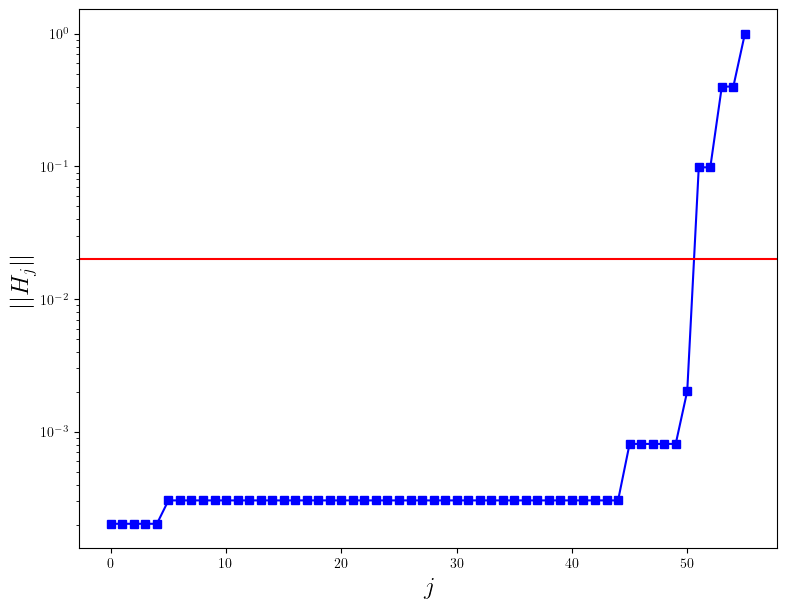
\includegraphics[width=1\textwidth]{J5dist.png}
            \caption{}
        \end{subfigure}
        \begin{subfigure}[b]{.49\textwidth}
            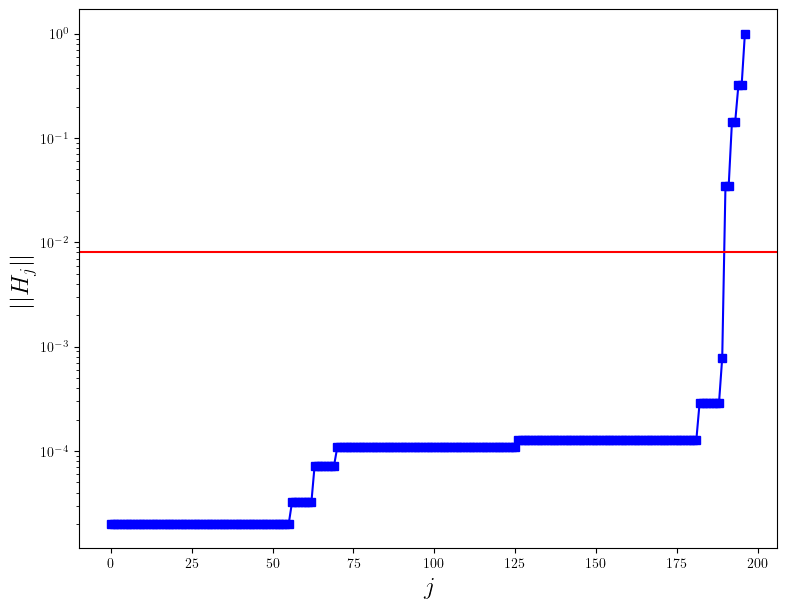
\includegraphics[width=1\textwidth]{J7dist.png}
            \caption{}
        \end{subfigure}
        \caption{\textit{Jellium Spectral Norm Distribution:} Semi-log plots of the sorted normalized spectral norms versus Hamiltonian index for 5 and 7 site Jellium models in figures (a) and (b) respectively. The plots show the increases in number of terms as well as how the distributions become increasingly sharply peaked. In red we provide a potential choice of $\omega_c$ for the partitioning heuristic.} \label{fig:Jelliumspec}
\end{figure}
\FloatBarrier

\subsubsection{Graph Hamiltonian Model}
The Hamiltonian we explore here involves a spin chain imposed on a lattice $\Gamma \in \mathbb{Z}^D$ with a graph distance metric $dist(\mathbf{u},\mathbf{v}) = |\mathbf{u}-\mathbf{v}|_1$ where $\mathbf{u}$ and $\mathbf{v}$ are vectorized coordinates on the graph with dimension equal to $D$. For our investigation we only examine lattices with $D=1$, given that for a fixed number of sites, this gives the most sharply peaked spectral distribution than any other $D$:

\begin{equation}
    H = \sum_{i>j} e^{-dist(i,j)}\alpha_{ij} \sigma^x_i \sigma^x_j + \sum_k \beta_k \sigma_k^z
\end{equation}

This system is similar to the quantum transverse field Ising model but with interactions that fall of exponentially with graph distance. The coefficients $\alpha_{ij}$ and $\beta_k$ are site dependant coupling constants that allow for the introduction of more disorder and/or structure in the Hamiltonian. To add some disorder to the model, we draw these coefficients pseudo-randomly from a Gaussian distribution with mean 0 and variance 1. \\

\subsubsection{Heisenberg Model}
The Heisenberg model describes a quantum spin system in a magnetic field with nearest-neighbour interactions. The Hamiltonian takes the following form:
\begin{equation} \label{eq:heisenberg}
    H = \sum_j \left(J_x \sigma_j^x \sigma_{j+1}^x + J_y \sigma_j^y \sigma_{j+1}^y + J_z \sigma_j^z \sigma_{j+1}^z \right)+ \sum_i B_z \sigma_i^z
\end{equation}
Here $B_z$ is the strength of the magnetic field in the $z$ direction and $J_{\{x, y, z\}}$ are coupling constants. Given the intuition of our composite channel, we expect this model to take advantage of our algorithm when the coupling constants largely differ in magnitude such that partitioning into Trotter and QDrift takes advantage of more Hamiltonian structure. Furthermore, introducing site-dependant coupling constants or writing down a highly disordered spin system could further add structure that the algorithm can take advantage of. A Hamiltonian of this nature would look something like the following: 
\begin{equation} \label{eq:spin_glass}
    H = \sum_j \left(J_x^{(j)} \sigma_j^x \sigma_{j+1}^x + J_y^{(j)} \sigma_j^y \sigma_{j+1}^y + J_z^{(j)} \sigma_j^z \sigma_{j+1}^z \right) + \sum_i B_z \sigma_i^z
\end{equation}
This Hamiltonian appears somewhat contrived for extracting the performance of the local composite channel. However, this system closely resembles the Edwards-Anderson model of a spin glass, a system of interest in condensed matter physics. In an attempt to create a sharp distribution, we simply sample $J_\nu^{(j)}$ from an exponential distribution with a scale parameter of 0.1. \\

\subsection{Partitioning Schemes} \label{sec:partition_scheme}
The main difficulty with deploying the composite simulation framework concerns  finding a good partitioning. In introducing composite simulations, Hagan and Wiebe suggested partitioning schemes derived on the basis of optimizing analytic cost functions both in deterministic and probabilistic settings \cite{hagan2022composite}. Here, we take a different approach involving the exact calculation of the simulation error, and an optimization routine that, given convergence, finds the optimal partitioning and gate count with respect to a chosen error tolerance and simulation time. This approach is used to answer the question regarding the best savings one can hope to achieve when deploying composite methods to simulate a specific Hamiltonian. We are not proposing this as a pre-processing routine (for a study of this nature see Ref. \cite{mc2023classically}), as it has complexity greater than that of the simulation itself, which is trivial as the optimization involves solving the simulation problem recursively. In addition, we also arrive at simple heuristics that can be used to partition certain Hamiltonians with little overhead, which we do propose as a strategy for using a composite approach. \\

\textit{Chop} is the partition that we introduce in this work. The idea is based on the heuristic of placing a few terms with larger spectral norms into Trotter-Suzuki channels and numerous small terms into QDrift, assuming that the Hamiltonian presents this structure. We start by sorting the terms by their spectral weights and introducing a ``chop threshold" $\omega_c \in [0, \max_i h_i]$. This scale will determine the partition such that if a term has spectral norm $h_i\geq\omega_c$ then $H_i\rightarrow A$ if $h_i < \omega_c$ then $H_i\rightarrow B$. Now we can express the error tolerance $\epsilon$ as a function of channel iterations $r$, with partitioning chop $\omega_c$ and a sample number $N_b$ that will be chosen in an optimization routine, and for a fixed initial state and time:
\begin{equation}\label{eq:errorfunc}
    \norm{(\mathcal{X}^{2k})^{\circ r}(\rho, t/r, \omega_c, N_b) - \evolchan{\rho, t}}_1 = \epsilon(r).
\end{equation}
%
By fixing an error tolerance for $\epsilon$, the exact cost of the simulation becomes a black box function with no closed form expression:
\begin{equation}\label{eq:cost_function}
    C_{comp} = f(\epsilon_{thresh}, r, \omega_c, N_b).
\end{equation}
This is the cost function we wish to minimize. However, we cannot do that by conventional methods such as with direct gradient descent. Also, with no strong intuition for a choice of $N_B$, if we wish to optimize this parameter we have to deal with integer optimization as well. The iterations $r$, however, while an integer, does not require optimization, but rather emits a search problem. If we allow an optimizer to pick initial random values for $N_b$ and $\omega_c$ from a fixed interval, then we must find the value $r$ required to meet the error threshold $\epsilon_{thresh}$, which will ultimately be determined by the optimizer's choice of the other two parameters. To complete this, we perform an exponential search on $r$ until we find some $r$ where $\epsilon(r) \geq \epsilon_{thresh}$ and set this as an upper bound on $r$. We then perform a binary search to find the smallest value of $r$ required to meet this condition and count the number of gates in the channel. This is a very expensive function given that we are precisely building the composite channel, applying it to the density matrix initial state in the problem, and counting the gates applied in each iteration of the search. The expensive nature emerges due to the sheer number of matrix multiplications required in performing this task, not in the search for $r$, which is nearly optimal. Note the importance of using the trace distance in this approach as it guarantees monotonicity of $\epsilon(r)$, which makes the search possible. This is not so in the framework of sampling the quantum infidelity, as finding the cost here would require other statistical methods (see Appendix \ref{sec:appendix_error}). \\
% DS3 The last sentence is unclear!
%MattP - slight change, and pointed the reader towards where this topic is further discussed.

Now a glaring question left unanswered is the choice of an optimizer. We implement the Gradient-Boosted Regression Trees (GBRT) algorithm included in Sci-Kit Optimize \cite{pedregosa2011scikit}. This algorithm is specifically-designed to handle the optimization of very expensive functions. It is also convenient for our purposes given that it can handle both integer and real optimization parameters simultaneously. At a high level, the algorithm works by using a series of decision trees with an associated loss function. The decision trees perform regression to fit the input function and are iteratively generated based on the minimization of the loss function via gradient descent. This optimizer and cost function \ref{eq:cost_function} can then be easily generalized to the local composite channels where now we have an $N_b$ and $\omega_c$ for each blocking. As the number of local blocks grows, the optimization routine will need to take a larger number of input parameters in this prescription. However, the size of the system becomes classically intractable long before we would consider using this many local blocks, so this is far from a concern. \\

In some cases, models may exhibit a partitioning that is somewhat canonical and can lead to excellent performance of composite methods. This occurs when we have a Hamiltonian that fits naturally into the intuition behind the algorithm, such that we have a set $A$ containing large terms with small commutators and a set $B$ with small terms that are known not to commute in general. We are, therefore, proposing to use the chop partition but by choosing the chop threshold $\omega_c$ based on physical intuition regarding the Hamiltonian, rather than some expensive optimization routine. A perfect example of such a system is a Heisenberg model with weak coupling. In this case, looking at Equation \ref{eq:heisenberg}, we would set the chop threshold $\omega_c = \max\{J_x, J_y, J_z\}$, which implies we simulate the interactions with QDrift $\{J_\nu \sigma_j^\nu \sigma_{j+1}^\nu\}_{\nu = x,y,z} \rightarrow B$, and simulate the site energy terms with Trotter-Suzuki $\{B_z \sigma_j^z\} \rightarrow A$. In this way, the terms in the set $A$ all commute with each other, whereas the terms in the set $B$ are guaranteed to have a small spectral norm. We bring numerical evidence that this provides computational advantages in the sections below. In general, any system with perturbative interactions may benefit from this framework, given that the commutators within the system are small, as they will avail  this canonical partitioning. In cases where the partitioning is not as obvious, as is the case with {\rm H$_3$} and Jellium, we can achieve similar advantages by choosing $\omega_c = \max \frac{d \norm{H_j}}{dj} \textbf{s.t.} \norm{B} \geq \norm{A}$, meaning we sweep an ordered list of the Hamiltonian spectral norms and track the largest difference between terms, chopping the list where this occurs, given $j\geq \frac{L}{2}$. The final condition is just to ensure the majority of terms are simulated by QDrift. We also use this strategy throughout \ref{subsec:performance} and show advantages. 

\subsection{Error Measures} \label{sec:Error_Measure}
In this investigation, there is some arbitrariness in the error measure one can choose in order to quantify the performance of a simulation channel. In order to evaluate the resources required by an algorithm, one must evaluate the number of gates required to meet a certain $\epsilon$, which is calculated by said error measure. In the literature, this $\epsilon$ is often quantified by the diamond distance utilized in previous sections. However, while analytically convenient, for any reasonably-sized system, computing this quantity becomes computationally expensive. While it is possible to evaluate it efficiently, this requires finding the solution of a semi-definite program, which is much less efficient than using some other error measures. In addition, since we are not constrained to analytically solvable expressions or closed form equations with our numerical methods, we can optimize this cost in terms of some partition scheme. This is the idea behind the optimal chop partition, and doing so requires frequent computations of $\epsilon$. With this in mind, the error of our algorithm should be a quantity that we can compute in a reasonable amount of time while also being a fair error measure. The criteria for ``fairness" comes within the error measures treating each algorithm that comprises the composite channel on an equal footing. For example, if we are to optimize the partitioning with respect to the gate cost (which is dependent on $\epsilon$), then if Trotter is more performant with respect to QDrift in one error measure than in another, then our composite optimizer will favor Trotter, which will be reflected in the partition. As a result the total cost of the composite channel will be skewed by the error measure used. \\

We consider the infidelity and trace distance as possible measures of $\epsilon$. For definitions and an additional discussion regarding the scaling and complexity of computing these quantities, see Appendix \ref{sec:appendix_error}. Analytics are required in order to answer the question of which measure might provide a more fair comparison. More specifically, we can ask the question of how the error measures will scale with respect to the total simulation time $t$, and then test these results numerically. In terms of the infidelity, we provide the following Theorems:
\begin{restatable}[QDrift Infidelity Time Scaling]{prop}{qdinfscaling} \label{thm:qdinfscaling}
    Given a QDrift channel $\qdchan{\rho, t}$ and the standard evolutionary channel $\capU(\rho, \nicefrac{t}{N})$, for a density matrix $\rho$, time $t/N$, then the infidelity between the outputs of the channels $1- \fidel(\qdchan{\rho, t}, \capU(\rho, t/N)) \in \bigo{t^2}$.
 \end{restatable}

 \begin{restatable}[Trotter-Suzuki Infidelity Time Scaling]{prop}{TSfidelity} \label{thm:TSfidelity}
Given a Trotter-Suzuki channel $\tschan{2k}{\rho, t}$ and the standard evolutionary channel $\evolchan{\rho, t}$, for a density matrix pure state $\rho$ and time $t$, then the infidelity between the outputs of the channels $1 - \fidel(\tschan{2k}{\rho, t} \capU(\rho, t)) \in \bigo{(t^{2k+1})^2}$.
\end{restatable}

The proofs of these theorems are included in  Appendix \ref{sec:appendix_error}. Here, we obtain the non-trivial result that the infidelity is squared when considering Trotter-Suzuki formulas. This would lead to our optimized chop algorithm to heavily favor this channel over QDrift, and for this reason, we consider it an "unfair" error measure. On the other hand, if we consider how the trace distance scales with simulation time in both algorithms, we obtain the following Theorems:

\begin{restatable}[QDrift Trace Distance Time Scaling]{prop}{QDtracedist} \label{thm:QDtracedist}
Given a QDrift channel $\qdchan{\rho, t}$ and the standard evolutionary channel $\capU(\rho, \nicefrac{t}{N})$, for an arbitrary density matrix $\rho$ and time $t/N$, then the trace distance between the outputs of the channels $\tracedist(\qdchan{\rho, t}, \capU(\rho, t/N)) \in \bigo{t^2}$.
\end{restatable}

\begin{restatable}[Trotter-Suzuki Trace Distance Time Scaling]{prop}{TStracedist} \label{thm:TStracedist}
    Given a Trotter-Suzuki channel $\tschan{2k}{\rho, t}$ and the standard evolutionary channel $\evolchan{\rho, t}$, for an arbitrary density matrix $\rho$ and time $t$, then the trace distance between the outputs of the channels $\tracedist(\tschan{2k}{\rho, t}, \capU(\rho, t)) \in \bigo{t^{2k+1}}$.
\end{restatable}

Here, we see that no such squaring occurs, and the expected time-scaling is obtained. For this reason, we compute the entire density matrix and  $\epsilon$ using the trace distance in all of our numerical simulations. Proofs of the above theorems, as well as further discussions can again be found in Appendix \ref{sec:appendix_error}.

\subsection{Performance Results} \label{subsec:performance}
In this section, we first numerically analyze the real time quantum algorithm given by Hagan and Wiebe \cite{hagan2022composite} and then show equivalent numerical calculations of the imaginary time classical case. To accomplish this, we provide cost plots in which we provide the minimum $C$, or the number of rotation gates to achieve a desired simulation accuracy $\epsilon$ (calculated by the trace distance) for each point in time $t$ or $\beta$. To reiterate, here we exactly compute entire evolution channels with a random initial state $\rho$ sampled from the unit hyper-sphere, and directly apply and count gates. We conclude this section with a brief discussion about numerical studies for the local composite simulation algorithms. In these plots, we study variants of the composite channel and display results with the aforementioned notation with the addition of a tilde over the channel if the partition and $N_B$ have been optimized with GBRT. 
% DS3 Was GBRT defined above? I may have missed that... MattP: yup!
For example, a composite channel with inner-order 2 and outer-order 1 with an optimized partition and number of QDrift samples $N_B$ is written like so $\widetilde{\mathcal{X}}^{2,1}$. Before presenting all of the results, for ease of reference, we find it useful to remind the reader of all relevant notations by summarizing them in the table below:\\
\begin{table}[htbp!] 
    \centering
    \begin{tabular}{| c | c | c | c |}
    \hline
        Notation & Description  \\
        \hline
        $C$ & Algorithmic cost defined in Section \ref{sec:cost_model} \\
        $t$ & Total Simulation time \\
        $\beta$ & Imaginary time/inverse temperature \\
        $r$ & Number of Channel iterations/time-steps \\
        $N_B$ & Number of QDrift samples \\
        $\mathcal{T}^{2k}$ & A Trotter-Suzuki channel of order $2k$  \\
        $\mathcal{Q}$ & A QDrift channel  \\
        $\mathcal{X}^{2k, 2g}$ & A Composite channel with inner-order $2k$ and outer-order $2g$ \\
        $\widetilde{\mathcal{X}}^{2k, 2g}$ & A Composite channel with partition and $N_B$ optimized by the GBRT algorithm \\
        $\mathcal{X}^{2k}_{l=j}$ & A Local Composite channel with inner-order $2k$ and block length $l=j$ \\
        \hline
    \end{tabular} 
    \caption{Summary of notation used in the numerical analysis, consistent with previous sections. The channels do not indicate whether we are working in real or imaginary time, however, that will be clear based on the subsections in which plots appear. This will also be the case for local channels simulating Hamiltonians defined on graphs.}
    \label{tab:notation}
\end{table} 

Throughout this section, we normalize $\norm{H} = 1$ and run simulations for times $t \in (0, \frac{3\pi}{2}]$ so as to ensure the system undergoes non-trivial dynamics without overlapping the phase. This is done due to the fact that Trotter formulas have a periodic error for $\norm{H}t\geq 2\pi$, and running simulations in this range would lead to the optimizer finding the ``good points", where the error happens to be small, which would provide a very low cost simulation and a sharp drop in the cost trend. We also report the cost advantages achieved on \textit{crossover points}, which are values of $t=t'$ such that $C_{QD}(t') = C_{TS}(t')$. We denote the composite channel \textit{crossover advantage} as 
\begin{equation} \label{eq:crossover}
    \xi \coloneqq C_{QD}(t') / C_\mathcal{X}(t') = C_{TS}(t') / C_\mathcal{X}(t'). 
\end{equation}
As we are unable to compute these times exactly we use interpolation methods to report values of $\xi$. This is motivated by the fact that analytics suggest this to be the point of greatest advantage for a composite channel \cite{hagan2022composite}. This is intuitive, especially given higher-order Trotter-Suzuki formulas which are known to asymptotically outperform QDrift for large $t$, whilst QDrift is dominant in the small $t$ limit, suggesting a region where their strengths can be combined. Therefore, studying $\xi$ is interesting in that it (given that our optimization scheme is convergent) represents the maximum advantage of using composite simulation algorithms. The value $t'$ at which $\xi$ appears may also suggest time scales for which composite algorithms are most advantageous. However, this analysis does not provide methods for finding $t'$ or predicting $\xi$ a priori as this is a very hard problem. The significance in $t'$ here lies in the fact that we always observe it to fall within the numerical domain of $t||H||\in (0, \frac{3\pi}{2}]$, which coincides with the domain suitable for quantum phase estimation, given we are implementing the real time algorithm. For imaginary time, these values can be viewed as relevant energy-time scales in which these formulas bring a computational benefit, rather than some physically interesting regime. Summarized in Table \ref{tab:numerics_results} are our calculated crossover advantages.

\begin{table}[htbp!]
    \centering
    \begin{tabular}{| c | c | c | c |}
    \hline
        Hamiltonian & $\xi$ & Num. Terms & Time \\
        \hline
        Hydrogen-3 & 2.3 & 62 & Real \\
        5 Site Jellium & 9.2 & 56 & Real \\
        6 Site Jellium & 18.8 & 94 & Real \\
        7 Site Jellium & 10.4 & 197 & Real \\
        7 Spin Graph & 4.1 & 49 & Real \\
        8 Spin Graph & 3.9 & 64 & Real \\
        \hline
        8 Spin Heisenberg & 3.1 & 29 & Imag. \\
        Hydrogen-3 & 2.3 & 62 & Imag. \\
        6 Site Jellium & 18.8 & 94 & Imag. \\
        \hline
    \end{tabular}
    \caption{Summary of gate cost improvements observed via the \textit{crossover advantage} $\xi$ defined in Equation \ref{eq:crossover} (contingent on optimization convergence). We observe that savings tend to somewhat improve as the number of terms increases (within the same model), with the exception of Jellium 7 where optimizer struggles with partitioning due to the number of terms. This is evident in the lack of monotonicity of $C(\widetilde{\mathcal{X}^1})$ in Figure \ref{fig:Jellium56}. The most significant savings are seen for the Jellium models. Even in cases where the number of terms are comparable to other models, larger advantages are persistent in Jellium. This is further establishes the spectral norm distribution as one of the most important indicators of performance in the composite framework.}
    \label{tab:numerics_results}
\end{table} 
\FloatBarrier

\subsubsection{Real-Time Composite Quantum Simulations}
Beginning with Hydrogen chains, our results are highlighted in Figure \ref{fig:H3}. This plot reveals two interesting features: for long-time simulations, heuristics can be found that essentially match the performance of an optimized formula simply by inspecting the distribution of the norms of individual summands $\norm{H_j}$, and with the optimized routine, we find a significant improvement at the crossover point with $\xi = 2.3$. These plots begin flat for most of the simulation channels, which for the most part, indicates that one application of the channel achieves the desired $\epsilon$ for multiple sequential simulations at small times. This is expected, and is especially common with Trotter-Suzuki formulas, given that with one iteration they apply at least $L$ gates depending on the order, while QDrift provides the option of sampling single gates.

\begin{figure}[htbp!]
    \centering
    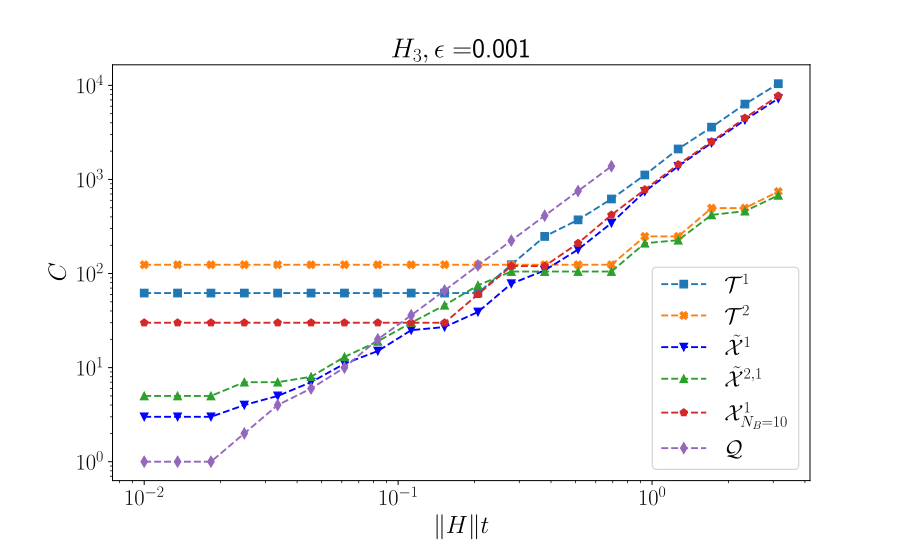
\includegraphics[width=0.6\textwidth]{H3update.png}
    \caption{\textit{H$_3$ Cost Plot Simulation (Real-Time): }Log-log gate cost plot for the {\rm H$_3$} Hamiltonian generated with OpenFermion using three-dimensional Gaussians in a minimal basis. The bond distance is chosen to be that which minimizes the energy surface of {\rm H$_2$}, which is $\approx 0.8$ angstrom. We achieve a crossover advantage of $\xi = 2.3$, as well as remaining constant factor advantages at long times. For other plot notations see Table \ref{tab:notation}.} \label{fig:H3}
\end{figure} 
\FloatBarrier

Figure \ref{fig:H3} is interesting given that both the heuristic and optimized channels provide significant advantages at the crossover point, as well as the heuristic partition seems to match the asymptotic performance of the optimized channel. This demonstrates that optimization subroutines are not required to gain advantages in this framework. Furthermore, the second inner-order composite channel also shows a consistent advantage over the second-order Trotter channel. \\

To gain insight into effective choices of partition and QDrift samples, we also plot the optimized $N_B$ values and the ratio of Trotter terms to total terms $|A|/|H|$ with time in Figure \ref{fig:H3nbW}. Here, we find choices that somewhat agree with our prior intuition. For short times, places almost all terms into QDrift, and slowly increases $N_B$. As $t$ increases, more terms are placed into Trotter with the partition bouncing around in the regime where Trotter and QDrift have similar costs, which is also expected. The composite channel $\widetilde{\mathcal{X}}^{2,1}$  essentially places all terms into the Trotter simulator, given the favorable asymptotic performance of higher order Trotter formulas over QDrift, while $\widetilde{\mathcal{X}}^{1}$ finds a balance between the two at long times, likely due to their equivalent $t$ scaling. The most interesting behavior is that of $N_B$ at mid to long times. Here, $N_B$ peaks near the crossover point and then falls off as Trotter $t$-scaling becomes dominant in $\widetilde{\mathcal{X}}^{2,1}$. However, for the $\widetilde{\mathcal{X}}^{1}$ channel, $N_B$ experiences somewhat of a revival after the peak, and stabilizes at 15, which is about 24\% of the terms. We use this percentage to motivate future heuristic choices of $N_B$ in our investigation of Jellium in Figure $\ref{fig:Jellium56}$, which turns out to work quite well. 

\begin{figure}[h!] 
    \centering
        \begin{subfigure}[b]{.49\textwidth}
            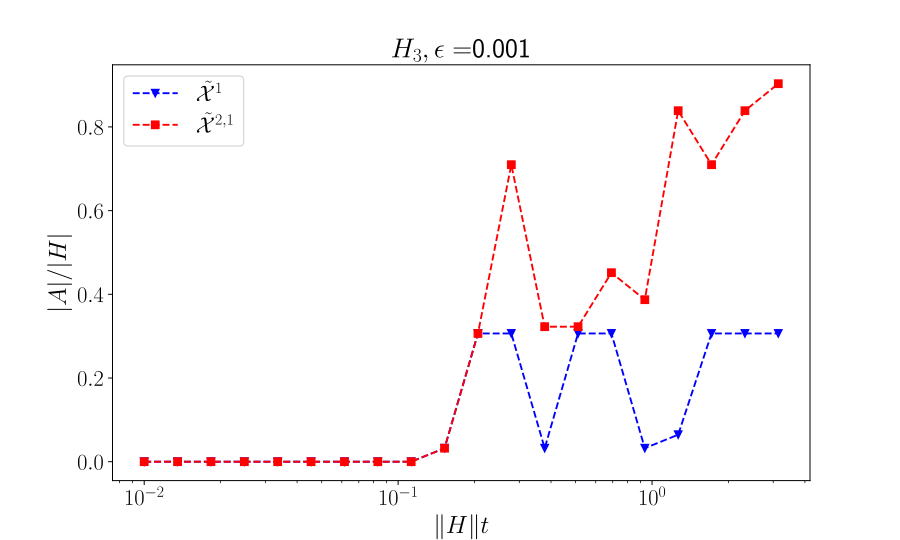
\includegraphics[width=1\textwidth]{H3_w.png}
            \caption{}
        \end{subfigure}
        \begin{subfigure}[b]{.49\textwidth}
            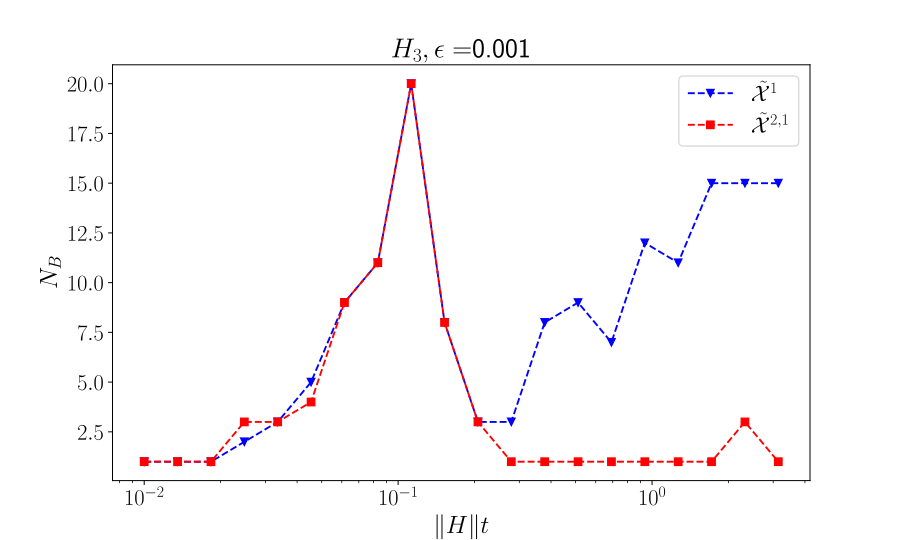
\includegraphics[width=1\textwidth]{H3_nb.png}
            \caption{}
        \end{subfigure}
        \caption{\textit{Optimized H$_3$ Simulation Parameters:} Semi-log plots of parameters obtained by the GBRT optimization routine for the $\widetilde{\mathcal{X}^{1}}$ and $\widetilde{\mathcal{X}}^{2,1}$ real time channels. These parameter choices correspond to the H$_3$ simulation in Figure \ref{fig:H3}. In (a) we plot the cardinality of the $A$ set over the total number of terms, as a function of time. These values are dictated by GBRT optimized value of $\omega_c$. In (b) we present the equivalent plot with $N_B$. For other plot notations see Table \ref{tab:notation}.} 
        \label{fig:H3nbW}
\end{figure}
\FloatBarrier

When it comes to the simulation of Jellium, we find some of the most significant performance improvements within this section, including an order of magnitude cost difference at the crossover point (see Figure \ref{fig:Jellium56}). Specifically, in the case of 6-site Jellium, the Trotter and QDrift cost at the crossover point is approximately 100 gates, versus the composite channel, which achieves the same precision $\epsilon$ with only about 7 gates. Here, it is also shown that one can find an adequate partition that leads to advantages at longer times without the need for any optimization. This is also the only model whereby the optimization routine struggles to find optimal partitions in the neighbourhood of the crossover point. This leads to the Jellium 7 model inheriting a smaller $\xi$ than what is likely achievable. 
\begin{figure}[h!]
    \centering
        \begin{subfigure}[b]{.49\textwidth}
            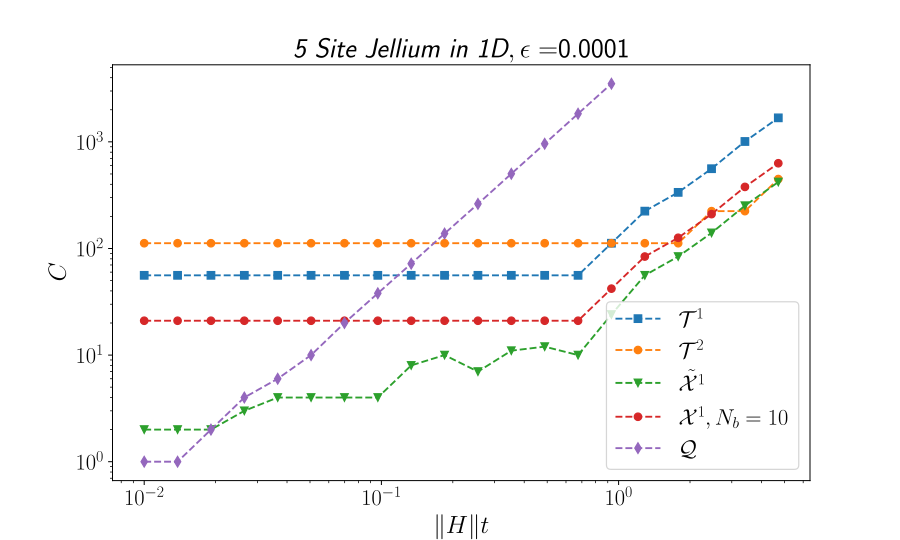
\includegraphics[width=1\textwidth]{Jellium5.png}
            \caption{}
        \end{subfigure}
        \begin{subfigure}[b]{.49\textwidth}
            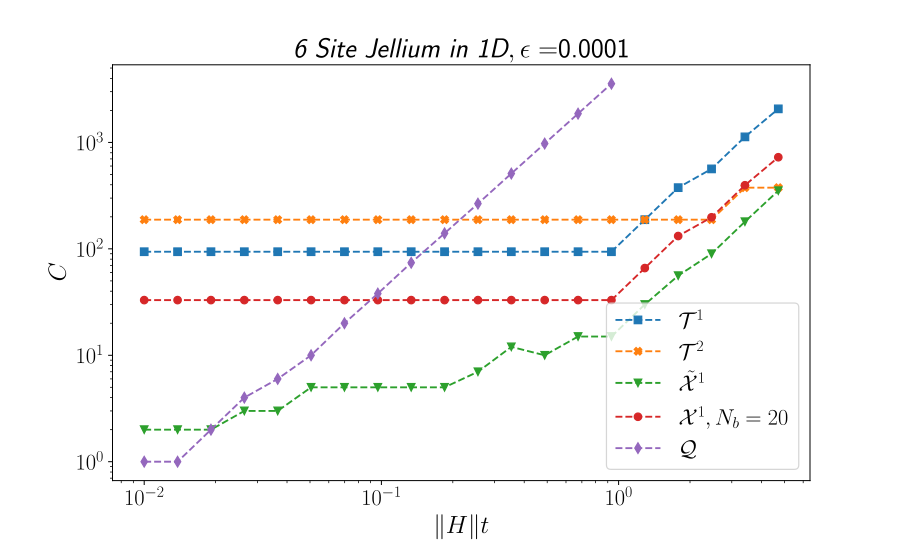
\includegraphics[width=1\textwidth]{Jellium6.png}
            \caption{}
        \end{subfigure}
        \begin{subfigure}[b]{.49\textwidth}
            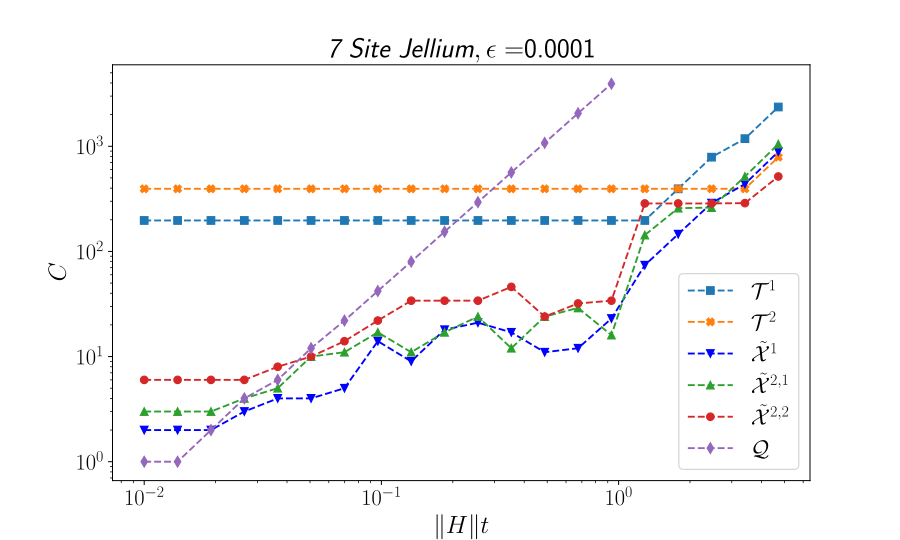
\includegraphics[width=1\textwidth]{Jellium7.png}
            \caption{}
        \end{subfigure}
        \caption{\textit{Jellium Simulation Cost plots (Real-time): } Log-log cost plots of quantum simulations of Jellium with 5, 6, and 7 sites in (a), (b), and (c) respectively. In (a) and (b) we have in red, a chop heuristic where no optimization overhead is used. The distribution of Hamiltonian terms is chopped immediately before $\max \frac{d \norm{H_j}}{dj}$, and approximately $\frac{1}{5}L$ terms are sampled. This heuristic works quite well, although it is outperformed by the optimized version, especially at short times. In (a) we achieve $\xi = 9.2$. In (b) we achieve an impressive advantage of $\xi =  18.8$, the largest of all our real time results. In (c), we perform a similar analysis of the 7 site model with some higher order composite channels, but find that the optimizer has increased difficulty with larger numbers of Hamiltonian terms. Here $\xi = 10.4$, but through inspecting some neighbouring points of the crossover region, it surely has the potentially to be much larger. For other plot notations see Table \ref{tab:notation}.} \label{fig:Jellium56}
\end{figure}
\FloatBarrier

The final system we investigate in this section is that of the graph toy model with exponentially decaying interactions, which is a beyond nearest neighbour model. In Figure \ref{fig:graph_sim}, we study this model for chains of length 7 and 8, and find essentially identical behaviour. When moving from 7 to 8 spins, we only add 15 more terms to the Hamiltonian, which is clearly not enough to see any significant advantages. In fact, the crossover advantage is slightly smaller for the bigger model, but this could also be due to the optimizer not fully converging. 

\begin{figure}[htbp!]
\centering
    \begin{subfigure}[b]{.49\textwidth}
        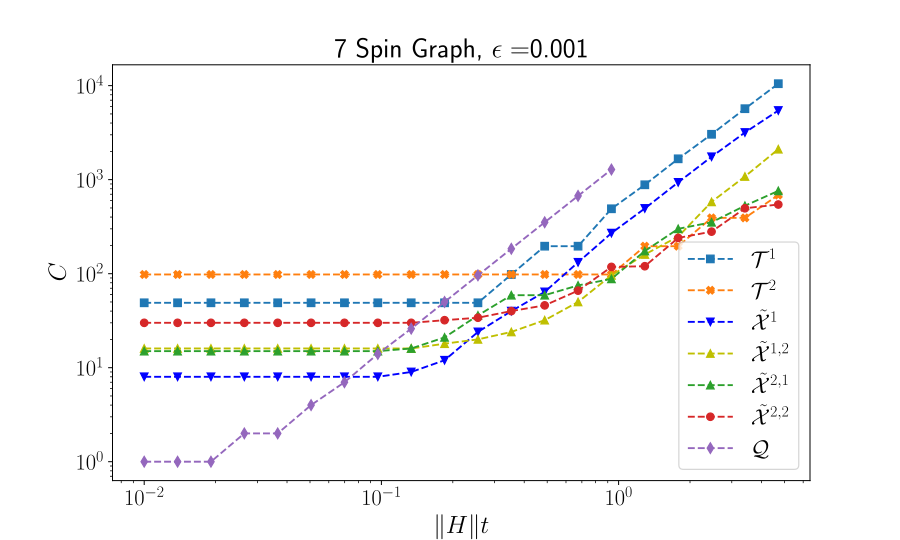
\includegraphics[width=1\textwidth]{graph7.png}
        \caption{} 
    \end{subfigure}
    \begin{subfigure}[b]{.49\textwidth}
        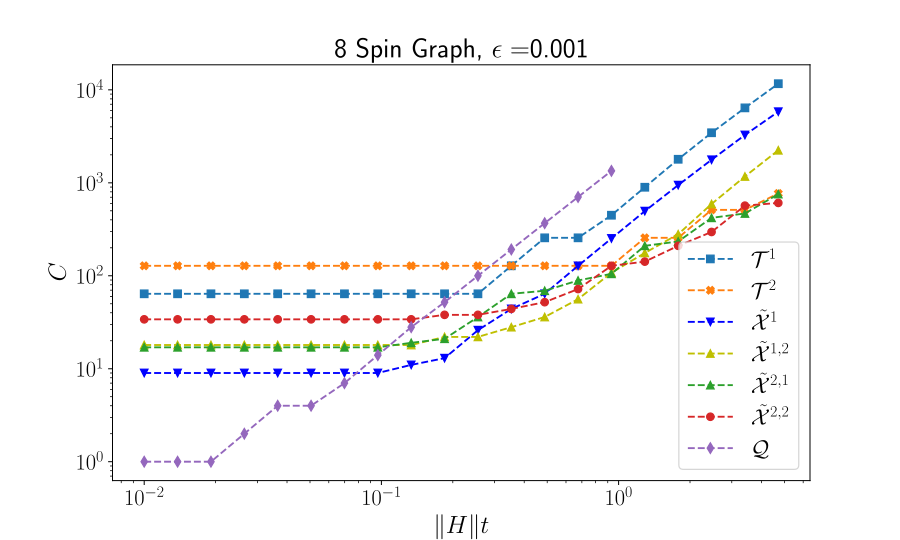
\includegraphics[width=1\textwidth]{graph8.png}
        \caption{} 
    \end{subfigure}
    \caption{\textit{Toy Spin Graph Model Cost Plot:} In (a) the we have a cost plot for the 7 spin model where we obtain a crossover advantage of $\xi = 4.1$, which is fairly significant. The plot has multiple regions where different composite channels are optimal. In (b) we have the 8 spin model where we establish $\xi = 3.9$. This advantage, as well as the channel performance is almost identical to (a). For other plot notations see Table \ref{tab:notation}.}
    \label{fig:graph_sim}
\end{figure} 
\FloatBarrier

\subsubsection{Imaginary-Time Composite Channels} \label{subsubsec:iTime_results}
This section contains cost plots of simulations of the same aforementioned Hamiltonians, but with imaginary time propagators, where we present cost plots of the most interesting Hamiltonians from the previous section.\\

For simulations of the Heisenberg model, we find similar advantages to those in real time. In Figure \ref{fig:imag_sim}, we see that our proposed heuristic leads to an advantage over Trotter-Suzuki and QDrift in the regions of interest. What is different about this plot is that the optimizer finds the same $N_B$ and partitioning for all short times. This is an artefact of both the Hamiltonian and how the optimizer is programmed. Since all the splitting (single site) terms have equal spectral norm, the optimizer is placed in an all or nothing scenario, as choosing $\omega_c < 1$ immediately places all terms into QDrift. Given that after receiving the cost, the program then solves a search problem to find the minimal $r$ to achieve $\epsilon$ precision, it is rare that it finds the ideal conditions to build a pure QDrift channel with $r=1$. However, significant savings are still achieved at the crossover point, and over $\mathcal{T}^1$ and $\mathcal{T}^2$ at large $\beta$. Once again, the validity of heuristic partitions are shown, specifically in the 1st order composite channel, which exactly matches its optimized version at large $\beta$. \\

\begin{figure}[htbp!]
    \centering
    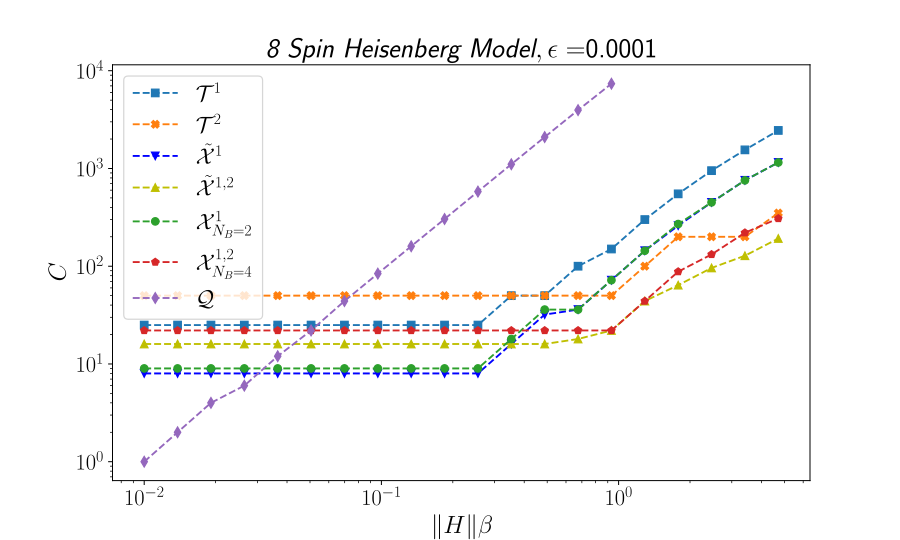
\includegraphics[width=0.7\textwidth]{iHeisenberg8.png}
    \caption{\textit{8 Spin Heisenberg Model Cost Plot:} In this imaginary time simulation we establish $\xi = 3.1$, as well as maintain advantages at large $\beta$. We also find that our chosen heuristics are essentially optimal at large $\beta$, with the green and dark blue lines overlapping. For other plot notations see Table \ref{tab:notation}.} \label{fig:imag_sim}
\end{figure} 
\FloatBarrier


For Hydrogen chains, we obtain strikingly similar results and compared with those in real time, as seen in Figure \ref{fig:iH3}. We once again obtain a significant crossover advantage, as well as constant factor advantages at large $\beta$, or low temperature. Heuristics are also shown to continue to hold in their effectiveness, in this case, from the crossover point and onward.

\begin{figure}[htbp!]
    \centering
    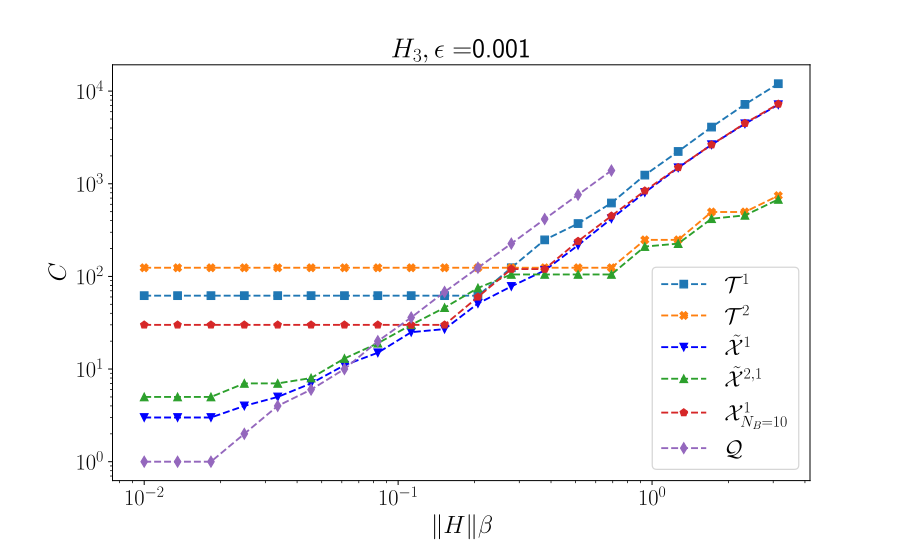
\includegraphics[width=0.7\textwidth]{iH3.png}
    \caption{\textit{H$_3$ Simulation Cost Plot (Imaginary-Time):} The same parameters are used to build the 3 atom Hydrogen chain as we done in real time. We achieve incredibly similar results, and again recover the real time result of $\xi = 2.3$ that was achieved in Figure \ref{fig:H3}. For other plot notations see Table \ref{tab:notation}.} \label{fig:iH3}
\end{figure} 
\FloatBarrier

For Jellium, we choose to investigate the system size with the best-behaved optimizer, as well as the largest $\xi$, which occurs for the 6-site model. In imaginary time, we once again reproduce a significant advantage, shown in Figure \ref{fig:iJellium6}. As in the case with {\rm H$_3$}, this plot is quite similar to the real time case in Figure \ref{fig:Jellium56}. However, here at large $\beta$ the composite channel seems to do better in imaginary time given that even the first order composite channel (with optimization) outperforms the second order Trotter channel. This happens in the final point of the plot where $\mathcal{T}^2$ is no longer in the``flat-regime". While this is very interesting, it is unclear analytically why this occurs, and we would likely not expect this trend to continue asymptotically. 

\begin{figure}[htbp!]
    \centering
    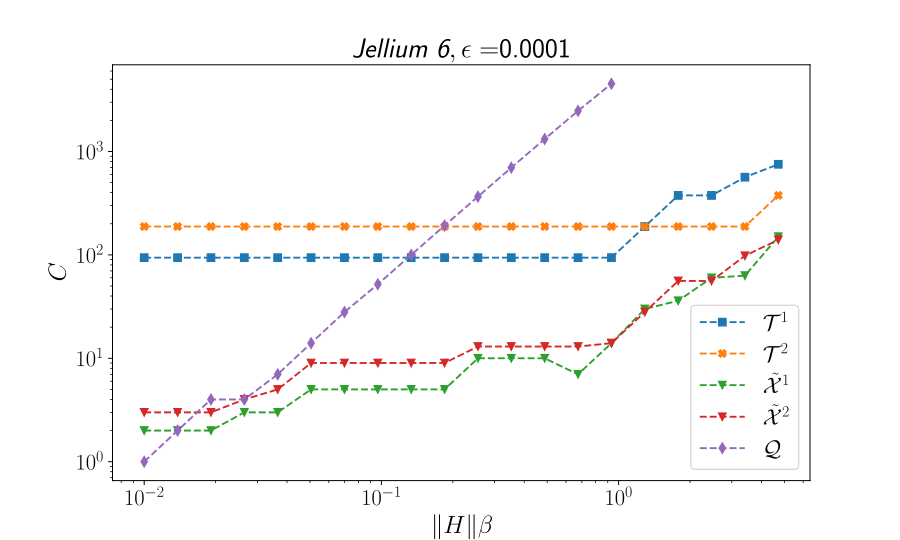
\includegraphics[width=0.7\textwidth]{iJellium6.png}
    \caption{\textit{6 Site Jellium Simulation Cost Plot (Imaginary-Time):} Here we recover the  crossover advantage of $\xi = 18.8$ from the real time simulation in Figure \ref{fig:Jellium56}, which is also the largest advantage achieved in our imaginary time simulations. We additionally achieve advantages over second order Trotter at large $\beta$. For other plot notations see Table \ref{tab:notation}.} \label{fig:iJellium6}
\end{figure} 
\FloatBarrier

Overall, this section nicely complements some of the analytics in Section \ref{sec:analysis} both by reinforcing the fact that composite quantum channels allow for similar advantages in both real and imaginary time, as well as through calculation of exact constant factor advantages. In other words, this section provides convincing evidence on the applicability of composite formulas to classical imaginary-time Monte-Carlo algorithms.


\subsubsection{Local Composite Quantum Channels}
Distinct from the previous two algorithms, with the local composite channels we do not immediately expect to see significant simulation advantages for the small systems we can compute. Recall, this algorithm makes use of the Lieb-Robinson velocity $v_{LR}$ that limits the propagation of information and thus correlations in a local lattice model. In our above numerics, our lattices contain $\leq 8$ sites, meaning even for small $v_{LR}$, the lattice can still become quickly entangled. In this section, it is important to understand where the observed advantages are originating, whether they are from the local decomposition, or something else. For example, the results in prior sections already suggest that composite channels can outperform Trotter and QDrift channels in certain regimes. If a block decomposition is introduced, we pay a small gate cost to break the simulation into subsets (as gates on the boundary are applied more than once), but the advantages of the composite simulation are almost guaranteed to outweigh this cost. Thus we wish to find a regime in which we can perform calculations of exact costs with local composite channels that explicitly gain advantages via block decomposition. Otherwise, we will observe essentially the same behaviour as before, but with slightly smaller constant factors. There are two ways to go about achieving this; one is to add more sites to the model, which quickly becomes computationally intractable with standard methods. The second strategy is to decrease the coupling between sites in the lattice, which naturally decreases $v_{LR}$. This is the strategy we utilize. In reference to Equation \ref{eq:heisenberg} we perform our cost plots on Heisenberg models with 8 sites with $B_z = 1$, and $J_\nu^{(j)}$ sampled from an exponential distribution with a scale parameter (serving as a coupling constant) of 0.00005. To allow for a fair simulation, we then choose $\epsilon = 0.000001$, such that statistically, $~98\% $ of terms will be greater than $\epsilon$, which can be seen from a simple integration of the PDF. Results of this simulation are shown in Figure \ref{fig:local_heisen}.  \\

\begin{figure}[htbp!]
    \centering
    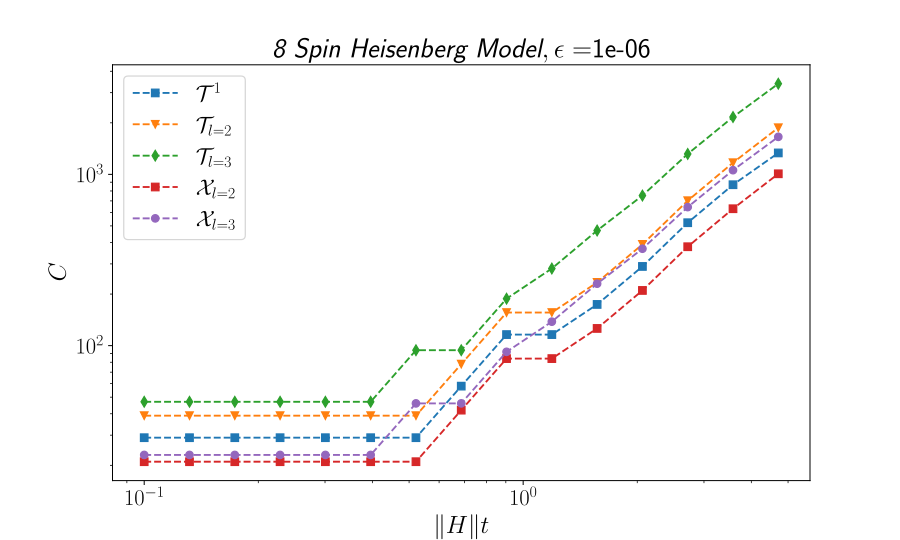
\includegraphics[width=0.7\textwidth]{local_Heisen8.png}
    \caption{\textit{8 Spin Heisenberg Model Simulated by localized and standard channels:} This cost plot compares Trotter to its  localized versions, with the subscript $l$ indicating the overlap of the boundary region in the block-local simulation.  Channels with no $l$ subscript are the standard simulations from prior sections. As expected, we observe that the composite channel is most efficient, however, given that the standard Trotter algorithm outperforms the localized Trotter channel, we can conclude that we are not in the regime where locality is providing advantages. The same heuristics were used for the composite channel as in Figure \ref{fig:imag_sim}, with $N_B = (4,1,4)$ on lattice subsets $(A, Y, B)$. For other plot notations see Table \ref{tab:notation}.} \label{fig:local_heisen}
\end{figure} 
\FloatBarrier

Given the gap between $\mathcal{T}^1$ and $\mathcal{T}_{l=2}$ in this very weak coupling regime, it is unclear whether our methods (exact gate counts) provide the means for investigating advantages gained by locality. In Ref. \cite{haah2021quantum}, via computations of bounds, numerics did not show advantages (in the form of T-gates) until approximately 100 sites were included in a more strongly-coupled model with $J_\nu^{(j)} \in [-1, 1]$ sampled i.i.d., so our results with far fewer spins are not unexpected. However, we still theoretically expect to see advantages in the limit where system sizes are large, and we can take advantage of the Lieb-Robinson bound.

    \chapter{Conclusion}
  \appendix
  \chapter{Appendix}


\section{Moment Bounds for Higher-Order Formulas} \label{sec:appendix_a}
We now return to proving the moment bounds from Section \ref{sec:higher_order_improvements}. 
\laSquared*
\begin{proof}
Given that the simplest definition of our probabilities is for $1-p_i$ we will try to work with expressions for the $B$ channel as much as possible. It is easy to convert between the two as
\begin{equation}
    \expect{L_A^2} = \expect{(L - L_B)^2} = L^2 -2L\expect{L_B} + \expect{L_B^2}.
\end{equation}
The expectation value of $L_B$ then follows from plugging in the definitions
\begin{equation}
    \expect{L_B} = \sum_i\expect{I_i^B} = \sum_i 1-p_i = \chi \sum_{i \in \probIndexSet} \frac{1}{h_i} + |\probIndexSet^C|. \label{eq:subPartLAsquare}
\end{equation}

Now we find a relatively simple upper bound for $\expect{L_B^2}$ if use the two facts that $I_i^B$ and $I_j^B$ are independent for $i \neq j$ and that $\parens{I_i^B}^2 = I_i^B$
\begin{align}
    \expect{L_B^2} &= \expect{\parens{\sum_i I_j^B}^2} \\
    &= \sum_i \expect{I_i^B} + \sum_{i \neq j} \expect{I_i^B}\expect{I_j^B} \\
    &= \sum_i (1-p_i) + \parens{\sum_i (1-p_i)}^2 - \sum_i (1-p_i)^2\\
    &= \chi \sum_{i \in \probIndexSet} \frac{1}{h_i} +|\probIndexSet^C| + \parens{\chi \sum_{i \in \probIndexSet} \frac{1}{h_i} +|\probIndexSet^C|}^2 - \sum_{i \in \probIndexSet} \frac{\chi^2}{h_i^2} - |\probIndexSet^C|. \label{eq:expectLBsquare}
\end{align}
Combining equations \eqref{eq:subPartLAsquare} and \eqref{eq:expectLBsquare} we get the following expression for an upper bound on $L_A^2$
\begin{align}
    \expect{L_A^2} &= L^2 - 2L(\chi \sum_{i \in \probIndexSet}\frac{1}{h_i} + |\probIndexSet^C|) + \chi \sum_{i \in \probIndexSet}\frac{1}{h_i} +\parens{\chi \sum_{i \in \probIndexSet}\frac{1}{h_i} + |\probIndexSet^C|}^2 - \sum_{i \in \probIndexSet} \frac{\chi^2}{h_i^2} \\
    &= L^2 -2L|\probIndexSet^C| + |\probIndexSet^C|^2 +  \parens{-2L + 1 + 2 |\probIndexSet^C|}\sum_{i \in \probIndexSet}\frac{\chi}{h_i} + \parens{\sum_{i \in \probIndexSet} \frac{\chi}{h_i}}^2 - \sum_{i \in \probIndexSet} \frac{\chi^2}{h_i^2} \\
    &= \parens{L - |\probIndexSet^C|}^2 +  \parens{1 - 2 |\probIndexSet|}\sum_{i \in \probIndexSet} \frac{\chi}{h_i} + \sum_{i \neq j \in \probIndexSet^2} \frac{\chi}{h_i} \frac{\chi}{h_j} \\
    &\leq |\probIndexSet|^2 + \parens{1 - 2|\probIndexSet|} \sum_{i \in \probIndexSet}\frac{\chi}{h_i} + \parens{|\probIndexSet| - 1} \sum_{i \in \probIndexSet} \frac{\chi}{h_i} \\
    &= |\probIndexSet|^2 - |\probIndexSet| \sum_{i \in \probIndexSet} \frac{\chi}{h_i}. \label{eq:LAasymptotic}
\end{align}
Note that we only used the following inequality $\frac{\chi}{h_i} = 1 - p_i \leq 1$ for $i \in \probIndexSet$. 
\end{proof}

\qUpperBounds*
\begin{proof}
$\expect{Q(t)}$ can be computed very similarly to $L_A$ above, since $\expect{Q(t)} \propto \expect{\lambda_B^2}$. This second moment for $\lambda_B$ mostly follows from the definitions but we first will get an easier expression involving the indicator variables
\begin{align}
    \expect{\lambda_B^2} &= \expect{\parens{\sum_i h_i I_i^B}^2} \\
    &= \sum_i h_i^2\expect{ I_i^B}  + \sum_{i \neq j} h_i h_j \expect{ I_i^B I_j^B} \\
    &= \sum_i h_i^2\expect{ I_i^B}  + \sum_{i \neq j} h_i \expect{ I_i^B} h_j \expect{I_j^B} \\
    &= \sum_i h_i^2\expect{ I_i^B}  + \parens{\sum_{i} h_i \expect{ I_i^B}}^2 - \sum_j h_j^2 \expect{I_j^B}^2,
\end{align}
where we used the fact that $I_i^B$ is independent from $I_j^B$ for all $i \neq j$. Now we can utilize our probability distributions as $\expect{I_i^B} = 1-p_i$, which yields
\begin{align}
    \expect{\lambda_B^2} &= \sum_{i \in \probIndexSet} h_i \chi + \sum_{i \in \probIndexSet^C} h_i^2 + \parens{\chi |\probIndexSet| + \lambda_{\probIndexSet^C}}^2 - \sum_{j \in \probIndexSet} h_j^2 (1-p_j)^2 - \sum_{j \in \probIndexSet^C} h_j^2 (1-p_j)^2 \\
    &= \lambda_{\probIndexSet} \chi + \sum_{i \in \probIndexSet^C} h_i^2 + \chi^2 |\probIndexSet|^2 + 2 \chi |\probIndexSet| \lambda_{\probIndexSet^C} + \lambda_{\probIndexSet^C}^2 - \chi^2 |\probIndexSet| - \sum_{j \in \probIndexSet^C} h_j^2 \\
    &\leq \chi^2 |\probIndexSet|^2 + \chi \parens{\lambda_{\probIndexSet} + 2 \lambda_{\probIndexSet^C} |\probIndexSet|} + \lambda_{\probIndexSet^C}^2 \\
    &=\chi \lambda_{\probIndexSet}  + \parens{\chi |\probIndexSet| + \lambda_{\probIndexSet^C}}^2. \label{eq:lambdaBsquared}
\end{align}
The only inequality comes from dropping the correction term $\chi^2 |\probIndexSet|$, which is subleading to $\chi^2 |\probIndexSet|^2$. 

Our expression for a upper bound on $\expect{Q(t)}$ is then proportional to the above expression \eqref{eq:lambdaBsquared}
\begin{equation}
    \expect{Q(t)} \leq \frac{2t^2}{N_B} \parens{\chi \lambda_{\probIndexSet}  + \parens{\chi |\probIndexSet| + \lambda_{\probIndexSet^C}}^2}.
\end{equation}
To compute $\expect{Q(t)^2}$ we can reduce it to our prior results. Since $\expect{Q(t)^2} = \frac{4 t^4}{N_B^2} \expect{\lambda_B^4}$, we will use the following upper bound
\begin{equation}
    \expect{\lambda_B^4} = \parens{\sum_i h_i I_i^B}^4 \leq \parens{\sum_i h_i 1}^2 \parens{\sum_i h_i I_i^B}^2 = \lambda^2 \expect{\lambda_B^2}.
\end{equation}
This means we can re-use the above computation as 
\begin{equation}
    \expect{Q(t)^2} \leq \frac{2t^2 \lambda^2}{N_B}\expect{Q(t)}. \label{eq:QsquaredAsymptotic}
\end{equation}
\end{proof}

\pUpperBound*
\begin{proof}
To simplify this we will use intermediate steps from the calculation of $P_{\max}(t)$ that bound the $\alpha_{comm}$ factors, namely equations \eqref{eq:alphaCommA}, \eqref{eq:alphaCommAB} which are repeated below
\begin{align}
    \alpha_{comm}(A, 2k) &\leq 2^{2k} \lambda_A^{2k+1} \\
    \alpha_{comm}(\set{A,B},2k) &\leq 2^{2k} \sum_{l=1}^{2k} \lambda_A^{l} \lambda_B^{2k+1 - l} \\
    P(t) &=  \frac{2^2 (t \Upsilon)^{2k + 1}}{2k+1} (\Upsilon \alpha_{comm}(A, 2k) + \alpha_{comm}(\set{A,B}, 2k))
\end{align}
We will use these to compute a useful upper bound on $\expect{P(t)}$. Since our random variables are more easily described for the $I_i^B$ variables, we will convert all powers of $\lambda_A$ into functions of $L$ and $\lambda_B$ as well as upper bound both by $\lambda_A$ and $\lambda_B$ by $\lambda$. This results in an upper bound on $\expect{P(t)}$ as
\begin{equation}
    \expect{P(t)} \leq \frac{2^{2 + 2k} (t \Upsilon)^{2k + 1}}{2k+1} \expect{\Upsilon \lambda_A^{2k+1} + \sum_{l=1}^{2k} \lambda_A^l \lambda_B^{2k+1-l}}. \label{eq:expectPbad}
\end{equation}
We will simplify the expectation value using the facts that $\lambda_A, \lambda_B \leq \lambda$ and that in $\sum_{l = 1}^{2k} \lambda_A^{l} \lambda_B^{2k + 1 - l}$ each term has at least one factor of $\lambda_A \lambda_B$. This results in the following simplifications
\begin{align}
    \expect{\Upsilon \lambda_A^{2k+1} + \sum_{l=1}^{2k} \lambda_A^l \lambda_B^{2k+1-l}} &\leq \lambda^{2k-1} \expect{\Upsilon \lambda_A^2 + (2k) \lambda_A \lambda_B} \\
    &\leq \Upsilon \lambda^{2k-1} \expect{\lambda_A^2 + \lambda_A \lambda_B} \\
    &= \Upsilon \lambda^{2k-1} \expect{\lambda_A(\lambda_A + \lambda_B)} \\
    &= \Upsilon \lambda^{2k} \parens{\lambda - \expect{\lambda_B}} \\
    &= \Upsilon \lambda^{2k} \parens{\lambda_{\probIndexSet} - \chi |\probIndexSet|}, \label{eq:exactUpperP}
\end{align}
where we used an exact expression for $\expect{\lambda_B}$ that is a straightforward computation in addition to the fact that $2k \leq \Upsilon$ for $k \geq 1$. Combining the above expressions \eqref{eq:exactUpperP} and \eqref{eq:expectPbad} our final expression for an upper bound on $\expect{P(t)}$ is 
\begin{equation}
    \expect{P(t)} \leq \frac{(2 \Upsilon)^{2 + 2k}}{2k+1} t^{2k+1} \lambda^{2k} \parens{\lambda_{\probIndexSet} - \chi |\probIndexSet|}
\end{equation}
\end{proof}


\section{Technical Proofs} \label{sec:appendix}
\subsection{Sinc Bounds} \label{sec:appendix_sinc}

\begin{lemma}[Sinc Function Bounds] \label{lem:sinc_poly_approx}
    For $\sinc^2\left( \frac{x t}{2} \right)$ and $\delta_{\min}$ as defined in Eq. \eqref{eq:delta_min_def}, we will make significant use of the following bounds:
    \begin{align}
        |x| \ge \delta_{\min} \implies \sinc^2 \left( \frac{x t}{2} \right) &\le \frac{4}{\delta_{\min}^2 t^2} \label{eq:sinc_upper_bound} \\
        |x| \le \frac{\sqrt{2}}{t} \implies \sinc^2\left(\frac{x t}{2} \right) &\ge 1 - \frac{|x|^2 t^2}{2}. \label{eq:sinc_lower_bound}
\end{align}

\end{lemma}
\begin{proof}
    The first inequality is rather trivial
    \begin{align}
        \sinc^2 \left( \frac{x t}{2} \right) &= \frac{\sin^2 (x t /2)}{(x t / 2)^2} \le \frac{4}{x^2 t^2} \le \frac{4}{\delta_{\min}^2 t^2}.
    \end{align}
    The second involves a Taylor Series for $\sinc^2$, which we compute using the expression of $\sinc$ as $\sinc(x t/ 2) = \frac{\sin xt /2}{xt/2} = \int_0^1 \cos(sxt/2) ds$.  The first two derivatives can then be computed easily
    \begin{align}
        \frac{d \sinc^2(x t /2)}{dx} &= - t \int_0^1 \sin(sx) s ds \int_0^1 \cos(sx) ds \\
        \frac{d^2 \sinc^2(x t /2)}{dx^2} &= -t^2 / 2 \int_0^1 \cos(sx)s^2 ds \int_0^1 \cos(sx) ds + t^2 / 2 \int_0^1 \sin(sx) s ~ds \int_0^1 \sin(sx) s ~ds.
    \end{align}
    We can evaluate each of these derivatives about the origin using continuity of the derivatives along with the limits $\lim_{x \to 0} \cos(sx) = 1$ and $\lim_{x \to 0} \sin(sx) = 0$. We can now compute the mean-value version Taylor series as
    \begin{align}
        \sinc^2 \left(\frac{x t}{2} \right) &= \sinc^2(0) + x \frac{d}{dx} \sinc^2 \left(\frac{x t}{2} \right) \bigg|_{x = 0} + \frac{x^2}{2!} \frac{d^2}{dx^2} \sinc^2 \left(\frac{x t}{2} \right) \bigg|_{x = x_{\star}},
    \end{align}
    where $x_{\star} \in [0,1]$. 
    Plugging in $\sinc^2(0) = 1$ and $\frac{d\sinc^2(x t /2)}{dx}\big|_{x = 0} = 0$ then yields $|\sinc^2(xt/2) - 1| = \frac{|x|^2}{2} \abs{\frac{d^2\sinc^2(x t / 2)}{dx^2}\big|_{x = x_{\star}}}$. We make use of the rather simplistic bound
    \begin{align}
        \abs{\frac{d^2\sinc^2(sxt/2)}{dx^2}\bigg|_{x = x_{\star}} } &\leq t^2 / 2 \abs{\int_0^1 \cos(sx_{\star} t/ 2) s^2 ds \int_0^1 \cos(sx_{\star} t/ 2) ds} + t^2 /2 \abs{\int_0^1 \sin(sx_{\star} t/ 2) s ds \int_0^1 \sin(sx_{\star} t/ 2) s ds} \\
        &\leq t^2 / 2 \int_0^1 \abs{\cos(sx_{\star} t/2)} s^2 ds \int_0^1 \abs{\cos(sx_{\star} t /2 )} ds + t^2 / 2 \parens{\int_0^1 \abs{\sin(sx_{\star} t /2)} |s| ds}^2 \\
        &\leq t^2 / 2 \int_0^1 s^2 ds + t^2 / 2 \parens{\int_0^1 s ds}^2 \\
        &\leq t^2.
    \end{align}
    This yields the final inequality $|\sinc^2(x t /2 ) - 1| \leq \frac{|x|^2 t^2}{2}$ which yields Eq. \eqref{eq:sinc_lower_bound}.
\end{proof}


\subsection{Haar Integral Proofs} \label{sec:haar_integral_appendix}

In this section we present the more technical work needed to state our results in Section \ref{sec:weak_coupling}. Lemmas \ref{lem:two_heisenberg_interactions} and \ref{lem:sandwiched_interaction} are used to compute the effects of the randomized interactions in a form that are usable in the main result of Lemma \ref{lem:big_one}. Lemma \ref{lem:haar_two_moment} can be derived from Appendix C in \cite{brandao2021complexity}.
\begin{restatable}{lemma}{haar_two_moment} \label{lem:haar_two_moment}
    Let $\int (\cdot) dU$ denote the average distributed according to the Haar measure over $\dim$-dimensional unitary matrices $U$. Then for $\ket{i_1},\ket{i_2},\ldots,\ket{k_2}$ drawn from an orthonormal basis
    \begin{align}
        &\int \bra{i_1} U \ket{j_1} \bra{i_2} U \ket{j_2} \bra{k_1} U^\dagger \ket{l_1} ~ \bra{k_2} U^\dagger \ket{l_2} dU \nonumber \\
        &= ~\frac{1}{\dim^2 - 1} \parens{\delta_{i_1, l_1} \delta_{j_1, k_1} \delta_{i_2, l_2} \delta_{j_2, k_2} + \delta_{i_1, l_2} \delta_{j_1, k_2} \delta_{i_2, l_1} \delta_{j_2, k_1}} \nonumber \\
        &\quad - \frac{1}{\dim(\dim^2 - 1)} \parens{\delta_{i_1, l_2} \delta_{j_1, k_1} \delta_{i_2, l_1} \delta_{j_2, k_2} + \delta_{i_1, l_1} \delta_{j_1, k_2} \delta_{i_2, l_2} \delta_{j_2, k_1}}. \label{eq:haar_two_moment_integral}
    \end{align}
\end{restatable}

\begin{lemma} \label{lem:two_heisenberg_interactions}
    Let $G(t)$ denote the Heisenberg evolved random interaction $G(t) = e^{iHt} G e^{-iHt}$ for a total Hamiltonian $H$. After averaging over the interaction measure the product $G(x) G(y)$ can be computed as
    \begin{equation}
        \int G(x) G(y) dG = \frac{1}{\dim + 1} \parens{\sum_{(i,j),(k,l)} e^{i \Delta(i,j|k,l) (x-y)} \ketbra{i,j}{i,j} + \identity}.
    \end{equation}
\end{lemma}
\begin{proof}
The overall structure of this proof is to evaluate the product in the Hamiltonian eigenbasis and split the product into three factors: a phase contribution from the time evolution, a Haar integral from the eigenvalues of the random interaction, and the eigenvalue contribution of the random interaction. Since this involves the use of multiple indices, it will greatly simplify the proof to use a single index over the total Hilbert space $\hilb$ as opposed to two indices over $\hilb_S \otimes \hilb_E$. For example, the index $a$ should be thought of as a pair $(a_s, a_e)$, and functions $\lambda(a)$ should be thought of as $\lambda(a_s, a_e)$. Once the final form of the expression is reached we will substitute in pairs of indices for easier use of the lemma in other places.
    \begin{align}
        \int G(x) G(y) dG &= \int e^{+i H x} U_G D U_G^\dagger e^{-i H x} e^{+i H y} U_G D U_G^\dagger e^{-i H y} dU_G ~dD \\
        &= \int \bigg[\sum_a e^{+i \lambda(a)x}\ketbra{a}{a}  U_G \sum_b D(b)\ketbra{b}{b} U_G^\dagger \nonumber \\
        &\quad \sum_c e^{-i \lambda(c) (x - y)} \ketbra{c}{c} U_G \sum_d D(d)\ketbra{d}{d} U_G^\dagger \sum_e e^{-i \lambda(e) y} \ketbra{e}{e} \bigg] dU_G ~dD\\
        &=\sum_{a,b,c,d,e} \ketbra{a}{e} e^{-i (\lambda(c) - \lambda(a))x} e^{-i (\lambda(e) - \lambda(c))y} \nonumber \\
        &\quad \times \int \bra{a} U_G \ket{b} \bra{c} U_G \ket{d} \bra{b} U_G^{\dagger} \ket{c} \bra{d} U_G^\dagger \ket{e} dU_G \int D(b) D(d) dD \\
        &=  \sum_{a, b, c, d, e} \delta_{bd} \ketbra{a}{e} e^{-i (\lambda(c) - \lambda(a))x} e^{-i (\lambda(e) - \lambda(c))y} \nonumber \\
        &\quad \times \int \bra{a} U_G \ket{b} \bra{c} U_G \ket{d} \bra{b} U_G^{\dagger} \ket{c} \bra{d} U_G^\dagger \ket{e} dU_G. \\
    \end{align}
    Now the summation over $d$ fixes $d=b$ and we use Lemma \ref{lem:haar_two_moment} to compute the Haar integral, which simplifies greatly due to the repeated $b$ index. Plugging the result into the above yields the following
    \begin{align}
        &= \frac{1}{\dim^2 - 1} \sum_{a, b, c, e} \ketbra{a}{e} e^{-i (\lambda(c) - \lambda(a))x} e^{-i (\lambda(e) - \lambda(c))y} \parens{\delta_{ac} \delta_{ce} + \delta_{ae} - \frac{1}{\dim} \parens{\delta_{ac} \delta_{ce} + \delta_{ae}}}  \\
        &= \frac{1}{\dim^2 - 1} \parens{1 - \frac{1}{\dim}} \sum_{a, b, c, e} \ketbra{a}{e} e^{-i (\lambda(c) - \lambda(a))x} e^{-i (\lambda(e) - \lambda(c))y} \delta_{ae} (1 + \delta_{ac}) \\
        &= \frac{1}{\dim^2 - 1} \parens{1 - \frac{1}{\dim}} \sum_{a, b, c} \ketbra{a}{a} e^{i (\lambda(a) - \lambda(c))(x-y)} (1 + \delta_{ac}) \\
        &= \frac{1 \parens{\dim - 1}}{\dim^2 - 1} \sum_{a,c} \ketbra{a}{a} e^{i (\lambda(a) - \lambda(c))(x - y)} (1 + \delta_{ac}) \\
        &= \frac{1}{\dim + 1} \parens{\sum_{a,c} e^{i (\lambda(a) - \lambda(c))(x-y)} \ketbra{a}{a} + \identity}.
    \end{align}
    Reindexing by $a \mapsto i,j$, $c \mapsto k,l$, and plugging in the definition of $\Delta$ yields the statement of the lemma.
\end{proof}


\begin{lemma} \label{lem:sandwiched_interaction}
    Given two Heisenberg evolved random interactions, $G(x)$ and $G(y)$, we compute their action on an outer-product $\ketbra{i,j}{k,l}$ as
    \begin{equation}
        \int G(x) \ketbra{i,j}{k,l} G(y) ~dG = \frac{1}{\dim + 1} \parens{\ketbra{i,j}{k,l} + \braket{i,j}{k,l} \sum_{m,n} e^{i \Delta(m,n | i,j) (x-y)} \ketbra{m,n}{m,n}}
    \end{equation}
\end{lemma}
\begin{proof}
This proof is structured the same as Lemma \ref{lem:two_heisenberg_interactions} and similarly we will use a single index of the total Hilbert space $\hilb$ and switch to two indices to match the rest of the exposition.
    \begin{align}
        \int G(x) \ketbra{a}{b} G(y) dG &=  \int e^{i H x} U_G D U_G^{\dagger} e^{-i H x} \ketbra{a}{b} e^{i H y} U_G D U_G^\dagger e^{-i H y} ~dG \\
        &= \sum_{c, d, e, f} e^{i (\lambda(c) - \lambda(a))x} e^{i (\lambda(b) - \lambda(f))y} \nonumber \\
        &\quad \times \int \ketbra{c}{c} U_G D(d) \ketbra{d}{d} U_G^\dagger \ketbra{a}{b} U_G D(e) \ketbra{e}{e} U_G^\dagger \ketbra{f}{f} dG \\
        &= \sum_{c, d, e, f}  e^{i (\lambda(c) - \lambda(a))x} e^{i (\lambda(b) - \lambda(f))y} \ketbra{c}{f} \nonumber \\
        &\quad \times \int D(d) D(e) dD \int \bra{c} U_G \ket{d} \bra{b} U_G \ket{e} \bra{d} U_G^\dagger \ket{a} \bra{e} U_G^\dagger \ket{f} dU_G \\
        &=  \sum_{c,d,f} e^{i (\lambda(c) - \lambda(a))x} e^{i (\lambda(b) - \lambda(f))y} \ketbra{c}{f} \nonumber \\ 
        &\quad \times \int \bra{c} U_G \ket{d} \bra{b} U_G \ket{d} \bra{a} \overline{U_G} \ket{d} \bra{f} \overline{U_G} \ket{d} dU_G \\
        &= \frac{1}{\dim^2 - 1} \sum_{c,d,f} e^{i (\lambda(c) - \lambda(a))x} e^{i (\lambda(b) - \lambda(f))y} \ketbra{c}{f} (\delta_{ca} \delta_{bf} + \delta_{cf}\delta_{ab})\parens{1 - \frac{1}{\dim}} \\
        &= \frac{1}{\dim + 1} \sum_{c,f} e^{i (\lambda(c) - \lambda(a))x} e^{i (\lambda(b) - \lambda(f))y} \ketbra{c}{f} (\delta_{ca} \delta_{bf} + \delta_{cf}\delta_{ab}) \\
        &= \frac{1}{\dim + 1} \parens{\ketbra{a}{b} + \delta_{ab} \sum_{c} e^{i(\lambda(c) - \lambda(a))(x-y)} \ketbra{c}{c} }.
    \end{align}
    Now re-indexing by $a \mapsto (i,j)$, $b \mapsto (k,l)$ and $c \mapsto (m,n)$ results in the expression given in the statement of the lemma.
\end{proof}


\secondOrderChannelHaar*
\begin{proof}
To start we would like to note that we will use a single index notation to refer to the joint system-environment eigenbasis during this proof to help shorten the already lengthy expressions. We will convert back to a double index notation to match the statement of the theorem. We start from the expression for the first derivative of the channel $\frac{\partial}{\partial \alpha} \Phi_G(\rho_S)$ given by Eq. \eqref{eq:first_order_alpha_derivative}. To take the second derivative there are six factors involving $\alpha$, so we will end up with six terms. We repeat Eq. \eqref{eq:first_order_alpha_derivative} below, add a derivative, and label each factor containing an $\alpha$ for easier computation
\begin{align}
    \frac{\partial^2}{\partial \alpha^2} \Phi_G(\rho_S) =& \frac{\partial}{\partial \alpha} \parens{\int_{0}^{1} \underset{\substack{\downarrow \\ (A)}}{e^{i s (H+\alpha G)t}} (i t G) \underset{\substack{\downarrow \\ (B)}}{e^{i (1-s) (H+\alpha G)t}} ds ~ \rho \underset{\substack{\downarrow \\ (C)}}{e^{-i(H+\alpha G)t}} } \nonumber \\
    &~ ~+\frac{\partial}{\partial \alpha} \parens{ \underset{\substack{\downarrow \\ (D)} }{e^{i(H+\alpha G)t}} \rho \int_{0}^1 \underset{\substack{\downarrow \\ (E)} }{e^{-i s (H+\alpha G) t} } (- i t G) \underset{\substack{\downarrow \\ (F)}}{e^{-i (1-s) (H+\alpha G)t}} ds }. \label{eq:second_derivative_labels}
\end{align}
Our goal is to get each of these terms in a form in which we can use either Lemma \ref{lem:two_heisenberg_interactions} or \ref{lem:sandwiched_interaction}. 
\begin{align}
    (A) &=i t\int_0^1 \parens{\frac{\partial}{\partial \alpha} e^{i s_1 (H+ \alpha G)t}} G e^{i(1-s_1)(H+\alpha G)t} ds_1 \rho e^{-i (H+\alpha G)t} \bigg|_{\alpha=0} \\
    &= (it)^2 \int_0^1 \parens{\int_0^1 e^{i s_1 s_2 (H+\alpha G)t} s_1 G e^{i s_1 (1-s_2) (H+\alpha G)t} ds_2} G e^{i(1-s_1) (H+\alpha G)t} ds_1 \rho e^{-i(H+\alpha G) t} \bigg|_{\alpha=0} \label{eq:second_order_deriv_intermediate_a}\\
    &= -t^2 \int_0^1 \int_0^1 e^{i s_1 s_2 H t} G e^{-i s_1 s_2 H t} e^{i s_1 H t} G e^{-i s_1 H t} s_1 ds_1 ds_2 e^{i H t} \rho e^{-i H t} \\
    &= -t^2 \int_0^1 \int_0^1 G(s_1 s_2 t) G(s_1 t) s_1 ds_1 ds_2 \rho(t). \label{eq:second_deriv_alpha_first_term}
\end{align}

\begin{align}
    (B) &= it \int_0^1 e^{i s_1 (H + \alpha G)t} G \frac{\partial}{\partial \alpha}\parens{e^{i(1-s_1)(H + \alpha G)t}} ds_1 \rho e^{-i(H + \alpha G) t} \bigg|_{\alpha = 0} \\
    &= (it)^2 \int_0^1 e^{i s_1 (H + \alpha G)t} G \parens{\int_0^1 e^{i(1-s_1)s_2 (H + \alpha G)t} (1-s_1) G e^{i(1 - s_1)(1 - s_2)(H + \alpha G)t} ds_2} ds_1 ~ \rho e^{-i ( H + \alpha G)t} \bigg|_{\alpha = 0} \\
    &= -t^2 \int_0^1 \int_0^1 e^{i s_1 H t} G e^{i(1-s_1)s_2 H t} G e^{i(1-s_1)(1-s_2) H t} (1-s_1) ds_1 ds_2 ~ \rho e^{-i H t}\\ 
    &= -t^2 \int_0^1 \int_0^1 e^{i s_1 H t} G e^{-i s_1 H t} e^{i(s_1 + s_2 - s_1 s_2) H t} G e^{-i (s_1 + s_2 - s_1 s_2) H t} (1-s_1) ds_1 ds_2 ~ \rho(t) \\
    &= -t^2 \int_0^1 \int_0^1 G(s_1 t) G((s_1 + s_2 - s_1 s_2)t) (1-s_1) ds_1 ds_2 ~ \rho(t)
\end{align}

\begin{align}
    (C) &= it \int_0^1 e^{i s (H + \alpha G)t} G e^{i(1-s) (H + \alpha G) t} ds ~\rho ~ \frac{\partial}{\partial \alpha} \parens{ e^{-i (H + \alpha G) t} } \bigg|_{\alpha = 0} \\
    &= (i t) (-it) \int_0^1 e^{i s (H + \alpha G)t} G e^{i (1 - s) (H + \alpha G)t} ds ~ \rho ~ \parens{ \int_0^1 e^{-i s (H + \alpha G)t} G e^{-i (1- s) ( H + \alpha G)t } ds}\bigg|_{\alpha = 0} \\
    &= + t^2 \parens{\int_0^1 e^{i s H t} G e^{-i s H t} ds} e^{i H t} \rho e^{-i H t} \parens{\int_0^1 e^{i (1-s) H t} G e^{-i (1-s) H t} ds} \\
    &= + t^2 \int_0^1 G(st) ds ~ \rho(t) \int_0^1 G((1-s)t) ds
\end{align}

\begin{align}
    (D) &= (-it) \frac{\partial}{\partial \alpha} \parens{e^{i(H + \alpha G)t}} \rho \int_0^1 e^{-i s (H + \alpha G)t} G e^{-i (1-s)(H + \alpha G)t} ds \bigg|_{\alpha = 0} \\
    &= t^2 \parens{\int_0^1 e^{i s (H+ \alpha G)t} G e^{i (1-s) (H + \alpha G)t}ds} \rho \int_0^1 e^{-i s (H + \alpha G)t} G e^{-i (1-s)(H + \alpha G)t} ds \bigg|_{\alpha = 0} \\
    &=  t^2 \int_0^1 e^{i s H t} G e^{-i s H t} ds ~\rho(t) \int_0^1 e^{i (1-s) H t} G e^{-i (1-s) H t} ds \\
    &= t^2 \int_0^1 G(st) ds ~ \rho(t) ~ \int_0^1 G((1-s)t) ds
\end{align}

\begin{align}
    (E) &= (-it) e^{i (H+ \alpha G) t} ~ \rho ~\int_0^1 \frac{\partial}{\partial \alpha} \parens{e^{-i s_1 (H + \alpha G)t}} G e^{-i (1-s_1)(H + \alpha G)t} ds_1 \bigg|_{\alpha = 0} \\
    &= - t^2 e^{i(H + \alpha G)t} ~ \rho ~\int_0^1 \parens{\int_0^1 e^{-i s_1 s_2 (H + \alpha G) t} (s_1 G) e^{-i s_1 (1-s_2) (H + \alpha G)t} ds_2} G e^{-i(1-s_1)(H + \alpha G)t} ds_1 \bigg|_{\alpha = 0} \\
    &= -t^2 e^{i H t} \rho e^{-i H t} \int_0^1 \int_0^1 e^{i (1 - s_1 s_2) H t} G e^{-i (s_1 - s_1 s_2)H t} G e^{-i (1-s_1)H t} s_1 ds_1 ds_2 \\
    &= -t^2 \rho(t) \int_0^1 \int_0^1 G((1- s_1 s_2) t) G((1-s_1)t) s_1 ds_1 ds_2
\end{align}

\begin{align}
    (F) &= (-it) e^{i(H + \alpha G) t} \rho \int_0^1 e^{-i s_1 ( H + \alpha G) t} G \frac{\partial}{\partial \alpha} \parens{ e^{-i (1-s_1) ( H +\alpha G)t}} ds_1 \bigg|_{\alpha = 0} \\
    &= (-it)^2 e^{i (H + \alpha G)t} \rho \int_0^1 e^{-i s_1 (H + \alpha G)t} G \parens{\int_0^1 e^{-i(1-s_1) s_2 (H + \alpha G)t} (1-s_1) G e^{-i(1-s_1) (1-s_2) (H + \alpha G) t} ds_2} ds_1 \bigg|_{\alpha = 0} \\
    &= -t^2 e^{-i H t} \rho e^{-i H t} \int_0^1 \int_0^1 e^{i (1- s_1) H t} G e^{-i (1-s_1) H t} e^{i (1-s_1)(1-s_2) H t} G e^{-i(1-s_1)(1-s_2) H t} (1-s_1) ds_1 ds_2 \\
    &= -t^2 \rho(t) \int_0^1 \int_0^1 G((1-s_1)t) G((1-s_1)(1 - s_2) t) (1-s_1)ds_1 ds_2
\end{align}

Now our goal is to compute the effects of averaging over the interaction $G$ on the above terms, starting with $(A)$. As this involves a lot of index manipulations, similarly to the proofs of Lemmas \ref{lem:two_heisenberg_interactions} and \ref{lem:sandwiched_interaction} we will use a single index for the total system-environment Hilbert space and switch back to a double index to state the results. We will make heavy use of Lemma \ref{lem:two_heisenberg_interactions}.
\begin{align}
    \int (A) dG &= -t^2 \int_0^1 \int_0^1 \int G(s_1 s_2 t) G(s_1 t) dG s_1 ds_1 ds_2 \rho(t) \\
    &= \frac{-t^2 }{\dim + 1} \int_0^1 \int_0^1 \parens{\sum_{i,j} e^{i (\lambda(i) - \lambda(j)) (s_1 s_2 t - s_1 t)} \ketbra{i}{i} + \identity} s_1 ds_1 ds_2 \rho(t) \\
    &= \frac{- t^2 }{\dim + 1} \parens{\sum_{i} \sum_{j : \lambda(i) \neq \lambda(j)} \int_0^1 \int_0^1 e^{i(\lambda(i) - \lambda(j))t (s_1 s_2 - s_1)} s_1 ds_1 ds_2 \ketbra{i}{i} + \sum_{i} \sum_{j : \lambda(i) = \lambda(j)}\frac{1}{2} \ketbra{i}{i} + \frac{1}{2} \identity} \rho(t) \\
    &= \frac{- t^2 }{\dim + 1} \parens{\sum_i \sum_{j : \lambda(i) \neq \lambda(j)} \frac{1 - i (\lambda(i) - \lambda(j))t - e^{-i (\lambda(i) - \lambda(j))t}}{t^2 (\lambda(i) - \lambda(j))^2} \ketbra{i}{i} + \frac{1}{2} \sum_{i} (\eta(i) + 1) \ketbra{i}{i} } \rho(t) \\
    &= \frac{- 1}{\dim + 1}\parens{\sum_{i} \sum_{j: \Delta_{ij} \neq 0} \frac{1 - i \Delta_{ij}t - e^{-i \Delta_{ij} t}}{\Delta_{ij}^2} \ketbra{i}{i} + \frac{t^2}{2} \sum_{i} (\eta(i) + 1)\ketbra{i}{i} } \rho(t)
\end{align}

We can similarly compute the averaged $(B)$ term:
\begin{align}
    \int (B) dG &= -t^2 \int_0^1 \int_0^1 \int G(s_1 t) G((s_1 + s_2 - s_1 s_2) t) dG (1-s_1) ds_1 ds_2 ~ \rho(t) \\
    &= \frac{- t^2 }{\dim + 1} \int_0^1 \int_0^1 \parens{\sum_{i,j} e^{i (\lambda(i) - \lambda(j))(s_1 s_2 - s_2) t} \ketbra{i}{i} + \identity} (1 -s_1) ds_1 ds_2 \rho \\
    &= \frac{- t^2 }{\dim + 1} \parens{\sum_{i} \sum_{j : \lambda(i) \neq \lambda(j)} \int_0^1 \int_0^1 e^{i(\lambda(i) - \lambda(j))t (s_1 s_2 - s_2)} (1 - s_1) ds_1 ds_2 \ketbra{i}{i} + \sum_{i} \sum_{j : \lambda(i) = \lambda(j)}\frac{1}{2} \ketbra{i}{i} + \frac{1}{2} \identity} \rho(t) \\
    &= \frac{- t^2 }{\dim + 1} \parens{\sum_i \sum_{j : \lambda(i) \neq \lambda(j)} \frac{1 - i (\lambda(i) - \lambda(j))t - e^{-i (\lambda(i) - \lambda(j))t}}{t^2 (\lambda(i) - \lambda(j))^2} \ketbra{i}{i} + \frac{1}{2} \sum_{i} (\eta(i) + 1) \ketbra{i}{i} } \rho(t) \\
    &= \frac{-1}{\dim + 1}\parens{\sum_{i} \sum_{j: \Delta_{ij} \neq 0} \frac{1 - i \Delta_{ij}t - e^{-i \Delta_{ij} t}}{\Delta_{ij}^2} \ketbra{i}{i} + \frac{t^2}{2} \sum_{i} (\eta(i) + 1)\ketbra{i}{i} } \rho(t),
\end{align}
which we note is identical to $\int (A) dG$. As terms $(C)$ and $(D)$ involve a different method of computation we skip them for now and compute $(E)$ and $(F)$. 
\begin{align}
    \int (E) dG &= -t^2 \rho(t) \int_0^1 \int_0^1 \int G((1- s_1 s_2) t) G((1-s_1)t) dG s_1 ds_1 ds_2 \\
    &= \frac{- t^2}{\dim + 1} \rho(t) \int_0^1 \int_0^1 \parens{\sum_{i,j} e^{i(\lambda(i) - \lambda(j)) t (s_1 - s_1 s_2)} \ketbra{i}{i} + \identity } s_1 ds_1 ds_2 \\
    &= \frac{- t^2}{\dim + 1} \rho(t) \parens{\sum_i \sum_{j : \lambda(i) \neq \lambda(j)} \frac{1 + i (\lambda(i) - \lambda(j))t - e^{i(\lambda(i) - \lambda(j))t}}{t^2 (\lambda(i) - \lambda(j))^2}\ketbra{i}{i} + \frac{1}{2} \sum_{i} (\eta(i) + 1 )\ketbra{i}{i}} \\
    &= \frac{- 1}{\dim + 1} \rho(t) \parens{\sum_i \sum_{j: (\Delta_{ij} \neq 0)} \frac{1 + i \Delta_{ij}t - e^{i\Delta_{ij}t}}{\Delta_{ij}^2} \ketbra{i}{i} + \frac{t^2}{2}\sum_i (\eta(i) + 1) \ketbra{i}{i}}.
\end{align}
Computing $(F)$ yields
\begin{align}
    \int (F) dG &= -t^2 \rho(t) \int_0^1 \int_0^1 \int G((1-s_1)t) G((1-s_1)(1 - s_2) t) dG (1-s_1)ds_1 ds_2 \\
    &= \frac{- t^2 \sigma ^2}{\dim + 1} \rho(t) \int_0^1 \int_0^1 \parens{\sum_{i,j} e^{i(\lambda(i) - \lambda(j))t (s_2 - s_1 s_2)}\ketbra{i}{i} + \identity} (1-s_1) ds_1 ds_2 \\
    &= \frac{- t^2 }{\dim + 1} \rho(t) \parens{\sum_{i} \sum_{j : \lambda(i) \neq \lambda(j)} \frac{1 + i (\lambda(i) - \lambda(j))t - e^{i (\lambda(i) - \lambda(j))t}}{t^2 (\lambda(i) - \lambda(j))^2} \ketbra{i}{i} +\frac{1}{2} \sum_{i} (\eta(i) + 1) \ketbra{i}{i}} \\
    &= \frac{- 1}{\dim + 1} \rho(t) \parens{\sum_i \sum_{j: (\Delta_{ij} \neq 0)} \frac{1 + i \Delta_{ij}t - e^{i\Delta_{ij}t}}{\Delta_{ij}^2} \ketbra{i}{i} + \frac{t^2}{2}\sum_i (\eta(i) + 1) \ketbra{i}{i}}
\end{align}
 which is identical to $\int (E) dG$.

 The last two terms $(C) = (D)$ are computed as follows:
 \begin{align}
     \int (C) dG &= t^2 \int_0^1 \int_0^1 \int G(s_1 t) \rho(t) G((1-s_2)t) ~dG ~ ds_1 ds_2 \\
     &= t^2 \sum_{i,j} \rho_{ij} e^{i(\lambda(i) - \lambda(j))t} \int_0^1 \int_0^1 \int G(s_1 t) \ketbra{i}{j} G((1-s_2)t) ~ dG ~ ds_1 ds_2 \\
     &= \frac{ t^2}{\dim + 1} \sum_{i,j} \rho_{ij} e^{i(\lambda(i) - \lambda(j))t} \parens{ \ketbra{i}{j} + \delta_{ij} \sum_{a} \int_0^1 \int_0^1 e^{i(\lambda(a) - \lambda(i))(s_1 + s_2 - 1)t} ds_1 ds_2 \ketbra{a}{a}} \\
     &= \frac{ t^2}{\dim + 1} \sum_{i,j} \rho_{ij} e^{i \Delta_{ij} t} \parens{\ketbra{i}{j} + \delta_{ij} \sum_{a : \Delta_{ai} \neq 0} \frac{2( 1- \cos (\Delta_{ai} t))}{\Delta_{ai}^2 t^2} \ketbra{a}{a} + \delta_{ij} \sum_{a : \Delta_{ai} = 0} \ketbra{a}{a}}
 \end{align}

 We can now combine each of these terms to offer the full picture of the output of the channel to second order. We make two modifications to the results from each sum: first, we will switch to double index notation to make for easier use in other areas, and secondly we let $\rho = \ketbra{i,j}{k,l}$. We note that the first term in the following equation is provided by $(A) + (B)$, the second through $(E) + (F)$, and the last two through $(C) + (D)$. 
 \begin{align}
     &\int \frac{\partial^2}{\partial \alpha^2} \Phi_G(\ketbra{i,j}{k,l})\bigg|_{\alpha = 0} dG \\
     &= -\frac{2  e^{i \Delta(i,j|k,l) t}}{\dim + 1} \bigg(\sum_{(a,b): \Delta(i,j|a,b) \neq 0} \frac{1 - i \Delta(i,j|a,b)t - e^{-i \Delta(i,j|a,b) t}}{\Delta(i,j|a,b)^2} \nonumber \\
     &~+ \sum_{(a,b): \Delta(k,l|a,b) \neq 0} \frac{1 + i \Delta(k,l|a,b) t - e^{i \Delta(k,l|a,b) t}}{\Delta(k,l|a,b)^2} + \frac{t^2}{2}(\eta(i,j) + \eta(k,l)) \bigg) \ketbra{i,j}{k,l} \nonumber \\
    &~ +\delta_{i,k} \delta_{j,l} \frac{2 e^{i \Delta(i,j|k,l)t}}{\dim+1} \parens{ \sum_{(a,b): \Delta(i,j|a,b) \neq 0 } \frac{2(1- \cos (\Delta(i,j|a,b)t))}{\Delta(i,j|a,b)^2} \ketbra{a,b}{a,b} + t^2 \sum_{(a,b) : \Delta(i,j|a,b) = 0} \ketbra{a,b}{a,b}} \label{eq:second_order_output}
 \end{align}
The last step we need is to use the half angle formula to change the cosine to a sine
\begin{align}
    \frac{2(1 - \cos(\Delta(i,j| a,b)t)}{\Delta(i,j|a,b)^2} &= \frac{2\left( 1 - \left(1 - 2 \sin^2\left(\frac{\Delta(i,j|a,b)t}{2} \right) \right) \right)}{\Delta(i,j|a,b)^2} \label{eq:trig_start} \\
    &= t^2 \frac{\sin^2 \left(\frac{\Delta(i,j|a,b) t}{2} \right)}{\frac{\Delta(i,j|a,b)^2 t^2}{4}} \\
    &= t^2 \sinc^2 \left(\frac{\Delta(i,j|a,b) t}{2 } \right), \label{eq:trig_end}
\end{align}
which yields the statement.


We can compute these by plugging in to Eq. \eqref{eq:el_gigante} again, which yields
\begin{align}s
&\int \bra{i', j'} \mathcal{T} \left( \ketbra{i, j}{i, j} \right) \ket{i', j'} ~dG = \begin{cases}        
\widetilde{\alpha}^2 \sinc^2(\Delta(i,j | i', j') t /2) & (i, j) \neq (i', j') \\
            - \widetilde{\alpha}^2 \sum_{(a,b) \neq (i, j)} \sinc^2(\Delta(a,b|i,j) t / 2) & (i,j) = (i', j')
        \end{cases}. \label{eq:system_environment_transitions}
    \end{align}
    The $(i, j) \neq (i', j')$ case should be apparent, the first term with the coherence factors $\chi$ are zero and the second term is what remains. The $(i,j) = (i', j')$ case can be seen as follows. For the first term we have
    \begin{align}
        - \frac{\alpha^2 e^{i \Delta(i,j| i,j) t}}{\dim + 1}\left(\chi(i,j) + \chi(i,j)^* + \frac{t^2}{2}(\eta(i,j) + \eta(i,j) \right) \ketbra{i,j}{i,j}.
    \end{align}
    We first compute the sum $\chi(i,j) + \chi(i,j)^*$ as
    \begin{align}
        \chi(i,j) + \chi(i,j)^* &= \sum_{a,b: \Delta(i,j,|a,b) \neq 0} \frac{1 - i \Delta(i,j|a,b)t - e^{-i \Delta(i,j|a,b) t}}{\Delta(i,j|a,b)^2} \nonumber\\
&\quad+ \sum_{a,b: \Delta(i,j,|a,b) \neq 0} \frac{1 + i \Delta(i,j|a,b)t - e^{+i \Delta(i,j|a,b) t}}{\Delta(i,j|a,b)^2} \\
    &= \sum_{a,b: \Delta(i,j| a,b) \neq 0} \frac{2 - e^{-i \Delta(i,j| a,b) t} - e^{+i \Delta(i,j| a,b) t}}{\Delta(i,j|a,b)^2} \\
    &= \sum_{a,b: \Delta(i,j| a,b) \neq 0} t^2 \sinc^2 \left( \frac{\Delta(i,j| a,b) t}{2} \right),
    \end{align}
    where the last step follows from a trigonometric identity (see Eqs. \eqref{eq:trig_start} - \eqref{eq:trig_end} in Appendix \ref{sec:haar_integral_appendix} for details). Since $\sinc(0) = 1$ the $\eta(i,j)$ term can be expressed as $\eta(i,j) = \sum_{a,b : \Delta(i,j|a,b) = 0} \sinc^2 \left( \frac{\Delta(i,j| a,b) t}{2} \right)$. Plugging this into Eq. \eqref{eq:el_gigante} gives
    \begin{align}
        &\int \bra{i,j} \mathcal{T} (\ketbra{i,j}{i,j}) \ket{i,j} dG \\
        &= \bra{i,j} \left(-\frac{\alpha^2 t^2}{\dim + 1} \sum_{a,b} \sinc^2 \left( \frac{\Delta(i,j| a,b) t}{2} \right) \ketbra{i,j}{i,j} + \sum_{a,b} \sinc^2\left( \frac{\Delta(i,j | a,b)t}{2} \right) \ketbra{a,b}{a,b} \right) \ket{i,j} \\
        &= -\frac{\alpha^2 t^2}{\dim + 1} \sum_{(a,b) \neq (i,j)} \sinc^2 \left( \frac{\Delta(i,j| a,b) t}{2} \right).
    \end{align}
    As a by-product of this computation we have just shown that $\trace{\mathcal{T}(\rho)} = 0$ and that our mapping is trace preserving to $\bigo{\alpha^2}$.
\end{proof}

\subsection{Weak-Coupling Remainder Bound} \label{sec:weak_coupling_remainder_bound}

\begin{proof}[Proof of Theorem~\ref{thm:remainder_bound}]
First we note that although $R_{\Phi}(\rho) = \frac{\alpha^3}{6} \partial_{\alpha}^3 \Phi(\rho)\big|_{\alpha = \alpha_{\star}}$ for a specific $ \alpha_{\star} > 0$ our proof will hold for any $\alpha_{\star}$. To compute the trace norm we will use the triangle inequality, unitary invariance of the Sch\"{a}tten norms, and submultiplicativity. To start,
\begin{align}
    \|\partial_\alpha^3 \Phi(\rho) \|_1 &= \left\| \frac{\partial^3}{\partial \alpha^3} {\rm Tr}_{H_E} \int e^{i(H+\alpha G)t} \rho_S \otimes \rho_E e^{-i(H+\alpha G)t} dG \bigg|_{\alpha = \alpha_{\star}} \right\|_1 \nonumber\\
    &= \left\| \frac{\partial^3}{\partial \alpha^3} {\rm Tr}_{H_E} \int e^{i(H+\alpha G)t} \rho_S \otimes \rho_E e^{-i(H+\alpha G)t} dG \bigg|_{\alpha = \alpha_{\star}} \right\|_1 \nonumber\\
    &\le    \int \left\|{\rm Tr}_{H_E}\frac{\partial^3}{\partial \alpha^3}\left( e^{i(H+\alpha G)t} \rho_S \otimes \rho_E e^{-i(H+\alpha G)t}\right) \bigg|_{\alpha = \alpha_{\star}} \right\|_1 dG.\label{eq:3derivBd}
\end{align}
To proceed, Proposition 1 of \cite{rastegin2012relations} allows us to eliminate the partial trace using the relation
$\norm{\partrace{\hilb_E}{X}}_{1} \le \norm{X}_{\dim_E} \le \norm{X}_1$. Further we use the decomposition of the second derivatives from the proof of Lemma \ref{lem:big_one}, specifically  Eq. \eqref{eq:second_derivative_labels} for the definition of each term, as $\partial_{\alpha}^2 \Phi_G = (A) + (B) + (C) + (D) +(E) + (F)$. This gives the following 
\begin{align}
    \norm{R_{\Phi}}_1 \le \frac{\alpha^3}{6} &\int \norm{\partial_{\alpha}((A) + (B) + (C) + (D) +(E) + (F)) \big|_{\alpha = \alpha_{\star}} }_1 dG \\
    &\le \frac{\alpha^3}{6} \int \norm{\partial_{\alpha}(A)\big|_{\alpha = \alpha_{\star}} }_1 + \norm{\partial_{\alpha}(B) \big|_{\alpha = \alpha_{\star}} }_1 + \ldots + \norm{\partial_{\alpha}(F) \big|_{\alpha = \alpha_{\star}} }_1 dG
\end{align}
We will demonstrate how this can be computed for the first term $\partial_{\alpha}(A)$. Using Eq. \eqref{eq:second_deriv_alpha_first_term}
\begin{align}
\partial_{\alpha} (A) &= -t^2 \partial_{\alpha} \int_0^1 \int_0^1 e^{i s_1 s_2 (H+\alpha G)t} G e^{i s_1 (1-s_2) (H+\alpha G)t} G e^{i(1-s_1) (H+\alpha G)t} \rho e^{-i(H+\alpha G) t}   s_1 ~ds_1 ds_2.
\end{align}
Due to the multiplication rule the resulting derivative will have 4 terms that each need one application of Duhamel's formula. We will show one of these terms, starting with the leftmost one
\begin{align}
    -t^2  &\int_0^1 \int_0^1 \partial_{\alpha} \left( e^{i s_1 s_2 (H+\alpha G)t} \right) G e^{i s_1 (1-s_2) (H+\alpha G)t} G e^{i(1-s_1) (H+\alpha G)t} \rho e^{-i(H+\alpha G) t}   s_1 ~ds_1 ds_2 \\
    = - i t^3  &\int_0^1 \int_0^1 \int_0^1 \left( e^{i s_1 s_2 s_3 (H+\alpha G)t} G e^{i s_1 s_2 (1 - s_3) (H+\alpha G)t} \right)\nonumber\\
    &\qquad\times G e^{i s_1 (1-s_2) (H+\alpha G)t} G e^{i(1-s_1) (H+\alpha G)t} \rho e^{-i(H+\alpha G) t}   s_1^2 s_2 ~ds_1 ds_2 ds_3.
\end{align}
Our goal is to compute the 1-norm of the above expression at $\alpha = \alpha_{\star}$. We can do so using the triangle inequality to move the norm of the matrices in the integrand. To proceed we will set $\alpha = \alpha_{\star}$ and reduce the norm of the matrices in the integrand using submultiplicativity and unitary invariance of the Sch\"{a}tten 1-norm as 
\begin{align}
    &\norm{\left( e^{i s_1 s_2 s_3 (H+\alpha_{\star} G)t} G e^{i s_1 s_2 (1 - s_3) (H+\alpha_{\star} G)t} \right) G e^{i s_1 (1-s_2) (H+\alpha_{\star} G)t} G e^{i(1-s_1) (H+\alpha_{\star} G)t} \rho e^{-i(H+\alpha_{\star} G) t}}_1 \\
    \le &\norm{e^{i s_1 s_2 s_3 (H+\alpha_{\star} G)t} G}_1 \norm{e^{i s_1 s_2 (1 - s_3) (H+\alpha_{\star} G)t} G}_1 \norm{e^{i s_1 (1-s_2) (H+\alpha_{\star} G)t} G}_1 \norm{e^{i(1-s_1) (H+\alpha_{\star} G)t} \rho e^{-i(H+\alpha_{\star} G) t}}_1 \\
    \le &\norm{G}_1^3 \norm{\rho}_1 = \norm{G}_1^3 .
\end{align}
Similar computations can be carried out for the other three terms for the derivative acting on $(A)$ which yields the inequality
\begin{align}
    \frac{\alpha^3}{6} \int \norm{\partial_{\alpha} (A)}_1 dG &\le \frac{\alpha^3 t^3}{6} \int \int_0^1 \int_0^1 \int_0^1 \norm{G}_1^3 (s_1^2 s_2 + s_1^2 (1 - s_2) + s_1(1-s_1) + s_1) ~ds_1 ds_2 ds_3 dG \\
    &\le \frac{4}{6} (\alpha t)^3 \int \norm{G}_1^3 dG . \label{eq:remainder_bound_on_A}
\end{align}

Now that we have computed the norm of the derivative acting on term $(A)$ we only have terms $(B)$ through $(F)$ to compute. These can all be checked to satisfy the same bound on $(A)$ from Eq. \eqref{eq:remainder_bound_on_A}, and as there are six terms in total we have the inequality
\begin{align}
    \norm{R_{\Phi}(\rho)}_1 &\le 4 (\alpha t)^3 \int \norm{G}_1^3 dG,
\end{align}
which we note holds for all inputs $\rho$. Therefore our last problem is to compute the expected norm of our interaction to the third power. We will decompose $G = U_{\text{Haar}} D U_{\text{Haar}}^\dagger $ to get
\begin{align}
    \int \norm{G}_1^3 dG &= \int \norm{D}_1^3 ~ dU_{\text{Haar}} dD = \sum_{i = 1}^{2 \dim_S} \int \abs{d_i}^3 dd_i = 2 \dim_S \mathbb{E}(\abs{y}^3),
\end{align}

where $y$ is a normal Gaussian random variable. This straightforwardly evaluates to $\mathbb{E}( |y|^3) = 2\sqrt{ \frac{2}{\pi}}$, yielding the final inequality
\begin{align}
    \norm{R_{\Phi}(\rho)}_1 \le 16 \sqrt{\frac{2}{\pi}} \dim_S (\alpha t)^3 ,
\end{align}
thus completing the proof.
\end{proof}


  \backmatter
  \printbibliography[heading=bibintoc]
\end{document}